\documentclass[a4paper]{book}
\usepackage{makeidx}
\usepackage{natbib}
\usepackage{graphicx}
\usepackage{multicol}
\usepackage{float}
\usepackage{listings}
\usepackage{color}
\usepackage{ifthen}
\usepackage[table]{xcolor}
\usepackage{textcomp}
\usepackage{alltt}
\usepackage{ifpdf}
\ifpdf
\usepackage[pdftex,
            pagebackref=true,
            colorlinks=true,
            linkcolor=blue,
            unicode
           ]{hyperref}
\else
\usepackage[ps2pdf,
            pagebackref=true,
            colorlinks=true,
            linkcolor=blue,
            unicode
           ]{hyperref}
\usepackage{pspicture}
\fi
\usepackage[utf8]{inputenc}
\usepackage{mathptmx}
\usepackage[scaled=.90]{helvet}
\usepackage{courier}
\usepackage{sectsty}
\usepackage[titles]{tocloft}
\usepackage{doxygen}
\lstset{language=C++,inputencoding=utf8,basicstyle=\footnotesize,breaklines=true,breakatwhitespace=true,tabsize=8,numbers=left }
\makeindex
\setcounter{tocdepth}{3}
\renewcommand{\footrulewidth}{0.4pt}
\renewcommand{\familydefault}{\sfdefault}
\hfuzz=15pt
\setlength{\emergencystretch}{15pt}
\hbadness=750
\tolerance=750
\begin{document}
\hypersetup{pageanchor=false,citecolor=blue}
\begin{titlepage}
\vspace*{7cm}
\begin{center}
{\Large txt\-Engine \\[1ex]\large v3.\-0 }\\
\vspace*{1cm}
{\large \-Generated by Doxygen 1.7.5.1}\\
\vspace*{0.5cm}
{\small Thu Sep 29 2011 12:02:21}\\
\end{center}
\end{titlepage}
\clearemptydoublepage
\pagenumbering{roman}
\tableofcontents
\clearemptydoublepage
\pagenumbering{arabic}
\hypersetup{pageanchor=true,citecolor=blue}
\chapter{\-Documentation for the txt\-Engine \-Project}
\label{index}\hypertarget{index}{}\hypertarget{index_date_sec}{}\section{\-Date Updated\-:}\label{index_date_sec}
29-\/11-\/2011\hypertarget{index_about_sec}{}\section{\-What is txt\-Engine?}\label{index_about_sec}
txt\-Engine is an interpreter for text only adventure games. \-Games are written using the \-X\-M\-L language making it easy for anyone to write and play their own games.\hypertarget{index_doc_sec}{}\section{\-Documentation\-:}\label{index_doc_sec}
\-To view the txt\-Engine \-Language \-Specification and \-Documentation click here\-: \href{../DocumentationMain.pdf}{\tt txt\-Engine \-Documentation}\hypertarget{index_links_sec}{}\section{\-Links\-:}\label{index_links_sec}

\begin{DoxyItemize}
\item txt\-Engine \-Project \-Site on \-Github\-: \href{https://github.com/smilefreak/txtEngine}{\tt https\-://github.\-com/smilefreak/txt\-Engine}\par



\item \-Tiny\-X\-M\-L \-Documentation\-: \href{http://www.grinninglizard.com/tinyxmldocs/index.html}{\tt http\-://www.\-grinninglizard.\-com/tinyxmldocs/index.\-html}\par
 
\end{DoxyItemize}\hypertarget{index_bugs_sec}{}\section{\-Report Bugs\-:}\label{index_bugs_sec}
\-Please report any bugs here\-: \href{https://github.com/smilefreak/txtEngine/issues}{\tt https\-://github.\-com/smilefreak/txt\-Engine/issues}\par
\hypertarget{index_author_sec}{}\section{\-Authors\-:}\label{index_author_sec}
\-Toby \-Herbert, \-Michael \-Abrams, \-James \-Boocock, \-Tatai \-Nikora 
\chapter{\-Deprecated \-List}
\label{deprecated}
\hypertarget{deprecated}{}

\begin{DoxyRefList}
\item[\label{deprecated__deprecated000002}%
\hypertarget{deprecated__deprecated000002}{}%
\-Member \hyperlink{class_ti_xml_handle_acb5fe8388a526289ea65e817a51e05e7}{\-Ti\-Xml\-Handle\-:\-:\-Element} () const ]use \-To\-Element. \-Return the handle as a \hyperlink{class_ti_xml_element}{\-Ti\-Xml\-Element}. \-This may return null.  
\item[\label{deprecated__deprecated000001}%
\hypertarget{deprecated__deprecated000001}{}%
\-Member \hyperlink{class_ti_xml_handle_ab44b723a8dc9af72838a303c079d0376}{\-Ti\-Xml\-Handle\-:\-:\-Node} () const ]use \-To\-Node. \-Return the handle as a \hyperlink{class_ti_xml_node}{\-Ti\-Xml\-Node}. \-This may return null.  
\item[\label{deprecated__deprecated000003}%
\hypertarget{deprecated__deprecated000003}{}%
\-Member \hyperlink{class_ti_xml_handle_a9fc739c8a18d160006f82572fc143d13}{\-Ti\-Xml\-Handle\-:\-:\-Text} () const ]use \-To\-Text() \-Return the handle as a \hyperlink{class_ti_xml_text}{\-Ti\-Xml\-Text}. \-This may return null.  
\item[\label{deprecated__deprecated000004}%
\hypertarget{deprecated__deprecated000004}{}%
\-Member \hyperlink{class_ti_xml_handle_a49675b74357ba2aae124657a9a1ef465}{\-Ti\-Xml\-Handle\-:\-:\-Unknown} () const ]use \-To\-Unknown() \-Return the handle as a \hyperlink{class_ti_xml_unknown}{\-Ti\-Xml\-Unknown}. \-This may return null. 
\end{DoxyRefList}
\chapter{\-Class \-Index}
\section{Class Hierarchy}
This inheritance list is sorted roughly, but not completely, alphabetically:\begin{DoxyCompactList}
\item \contentsline{section}{Area}{\pageref{class_area}}{}
\item \contentsline{section}{AreaCommand}{\pageref{class_area_command}}{}
\item \contentsline{section}{Item}{\pageref{class_item}}{}
\item \contentsline{section}{ItemCommand}{\pageref{class_item_command}}{}
\item \contentsline{section}{StateDescriptor}{\pageref{class_state_descriptor}}{}
\item \contentsline{section}{TiXmlAttributeSet}{\pageref{class_ti_xml_attribute_set}}{}
\item \contentsline{section}{TiXmlBase}{\pageref{class_ti_xml_base}}{}
\begin{DoxyCompactList}
\item \contentsline{section}{TiXmlAttribute}{\pageref{class_ti_xml_attribute}}{}
\item \contentsline{section}{TiXmlNode}{\pageref{class_ti_xml_node}}{}
\begin{DoxyCompactList}
\item \contentsline{section}{TiXmlComment}{\pageref{class_ti_xml_comment}}{}
\item \contentsline{section}{TiXmlDeclaration}{\pageref{class_ti_xml_declaration}}{}
\item \contentsline{section}{TiXmlDocument}{\pageref{class_ti_xml_document}}{}
\item \contentsline{section}{TiXmlElement}{\pageref{class_ti_xml_element}}{}
\item \contentsline{section}{TiXmlText}{\pageref{class_ti_xml_text}}{}
\item \contentsline{section}{TiXmlUnknown}{\pageref{class_ti_xml_unknown}}{}
\end{DoxyCompactList}
\end{DoxyCompactList}
\item \contentsline{section}{TiXmlCursor}{\pageref{struct_ti_xml_cursor}}{}
\item \contentsline{section}{TiXmlHandle}{\pageref{class_ti_xml_handle}}{}
\item \contentsline{section}{TiXmlParsingData}{\pageref{class_ti_xml_parsing_data}}{}
\item \contentsline{section}{TiXmlString}{\pageref{class_ti_xml_string}}{}
\begin{DoxyCompactList}
\item \contentsline{section}{TiXmlOutStream}{\pageref{class_ti_xml_out_stream}}{}
\end{DoxyCompactList}
\item \contentsline{section}{TiXmlVisitor}{\pageref{class_ti_xml_visitor}}{}
\begin{DoxyCompactList}
\item \contentsline{section}{TiXmlPrinter}{\pageref{class_ti_xml_printer}}{}
\end{DoxyCompactList}
\item \contentsline{section}{World}{\pageref{class_world}}{}
\end{DoxyCompactList}

\chapter{\-Class \-Index}
\section{\-Class \-List}
\-Here are the classes, structs, unions and interfaces with brief descriptions\-:\begin{DoxyCompactList}
\item\contentsline{section}{\hyperlink{class_area}{\-Area} }{\pageref{class_area}}{}
\item\contentsline{section}{\hyperlink{class_area_command}{\-Area\-Command} }{\pageref{class_area_command}}{}
\item\contentsline{section}{\hyperlink{classcombine}{combine} }{\pageref{classcombine}}{}
\item\contentsline{section}{\hyperlink{class_item}{\-Item} }{\pageref{class_item}}{}
\item\contentsline{section}{\hyperlink{class_item_command}{\-Item\-Command} }{\pageref{class_item_command}}{}
\item\contentsline{section}{\hyperlink{class_state_descriptor}{\-State\-Descriptor} }{\pageref{class_state_descriptor}}{}
\item\contentsline{section}{\hyperlink{class_world}{\-World} }{\pageref{class_world}}{}
\end{DoxyCompactList}

\chapter{\-File \-Index}
\section{File List}
Here is a list of all documented files with brief descriptions:\begin{DoxyCompactList}
\item\contentsline{section}{/home/cshome/m/mabrams/345/txtEngine/{\bfseries .\_\-Area.h} }{\pageref{_8___area_8h}}{}
\item\contentsline{section}{/home/cshome/m/mabrams/345/txtEngine/{\bfseries .\_\-AreaCommand.h} }{\pageref{_8___area_command_8h}}{}
\item\contentsline{section}{/home/cshome/m/mabrams/345/txtEngine/{\bfseries .\_\-Item.h} }{\pageref{_8___item_8h}}{}
\item\contentsline{section}{/home/cshome/m/mabrams/345/txtEngine/{\bfseries .\_\-ItemCommand.h} }{\pageref{_8___item_command_8h}}{}
\item\contentsline{section}{/home/cshome/m/mabrams/345/txtEngine/{\bfseries .\_\-parser.h} }{\pageref{_8__parser_8h}}{}
\item\contentsline{section}{/home/cshome/m/mabrams/345/txtEngine/{\bfseries .\_\-StateDescriptor.h} }{\pageref{_8___state_descriptor_8h}}{}
\item\contentsline{section}{/home/cshome/m/mabrams/345/txtEngine/{\bfseries .\_\-World.h} }{\pageref{_8___world_8h}}{}
\item\contentsline{section}{/home/cshome/m/mabrams/345/txtEngine/\hyperlink{_area_8cpp}{Area.cpp} (The \hyperlink{class_area}{Area} Class )}{\pageref{_area_8cpp}}{}
\item\contentsline{section}{/home/cshome/m/mabrams/345/txtEngine/\hyperlink{_area_8h}{Area.h} (Describes the \hyperlink{class_area}{Area} Class )}{\pageref{_area_8h}}{}
\item\contentsline{section}{/home/cshome/m/mabrams/345/txtEngine/\hyperlink{_area_command_8cpp}{AreaCommand.cpp} (The \hyperlink{class_area_command}{AreaCommand} Class )}{\pageref{_area_command_8cpp}}{}
\item\contentsline{section}{/home/cshome/m/mabrams/345/txtEngine/\hyperlink{_area_command_8h}{AreaCommand.h} (Describes the \hyperlink{class_area_command}{AreaCommand} Class )}{\pageref{_area_command_8h}}{}
\item\contentsline{section}{/home/cshome/m/mabrams/345/txtEngine/\hyperlink{_item_8h}{Item.h} (Describes the \hyperlink{class_item}{Item} Class )}{\pageref{_item_8h}}{}
\item\contentsline{section}{/home/cshome/m/mabrams/345/txtEngine/\hyperlink{_item_command_8h}{ItemCommand.h} (Describes the \hyperlink{class_item_command}{ItemCommand} Class )}{\pageref{_item_command_8h}}{}
\item\contentsline{section}{/home/cshome/m/mabrams/345/txtEngine/\hyperlink{parser_8h}{parser.h} (Describes the Parser Class )}{\pageref{parser_8h}}{}
\item\contentsline{section}{/home/cshome/m/mabrams/345/txtEngine/\hyperlink{_state_descriptor_8h}{StateDescriptor.h} (Describes the \hyperlink{class_state_descriptor}{StateDescriptor} Class )}{\pageref{_state_descriptor_8h}}{}
\item\contentsline{section}{/home/cshome/m/mabrams/345/txtEngine/{\bfseries tinystr.h} }{\pageref{tinystr_8h}}{}
\item\contentsline{section}{/home/cshome/m/mabrams/345/txtEngine/{\bfseries tinyxml.h} }{\pageref{tinyxml_8h}}{}
\item\contentsline{section}{/home/cshome/m/mabrams/345/txtEngine/\hyperlink{_world_8h}{World.h} (Describes the \hyperlink{class_world}{World} Class )}{\pageref{_world_8h}}{}
\end{DoxyCompactList}

\chapter{\-Class \-Documentation}
\hypertarget{class_area}{
\section{Area Class Reference}
\label{class_area}\index{Area@{Area}}
}
\subsection*{Public Member Functions}
\begin{DoxyCompactItemize}
\item 
\hypertarget{class_area_a928ac4f85119316a126beafc575a5f84}{
bool {\bfseries has\_\-description} (std::string desc\_\-id)}
\label{class_area_a928ac4f85119316a126beafc575a5f84}

\item 
\hypertarget{class_area_ac3f89059fe2ef23610dc3a5650c94c0d}{
std::string {\bfseries get\_\-status} ()}
\label{class_area_ac3f89059fe2ef23610dc3a5650c94c0d}

\item 
\hypertarget{class_area_a7a2701d4527e084ea7f8944925b539d7}{
bool {\bfseries has\_\-current\_\-desc} ()}
\label{class_area_a7a2701d4527e084ea7f8944925b539d7}

\item 
\hypertarget{class_area_aee8135f25247d5e06dc0b28bf8cabcba}{
int {\bfseries get\_\-num\_\-items} ()}
\label{class_area_aee8135f25247d5e06dc0b28bf8cabcba}

\item 
\hypertarget{class_area_acab405d06547438ee02b3d8b9a2ff013}{
std::string {\bfseries get\_\-description} ()}
\label{class_area_acab405d06547438ee02b3d8b9a2ff013}

\item 
\hypertarget{class_area_a687234da51ac6da40d2aee426926dfcd}{
void {\bfseries remove\_\-item} (int index)}
\label{class_area_a687234da51ac6da40d2aee426926dfcd}

\item 
\hypertarget{class_area_a8f4693277743a9dbc6ac0212fc02c86f}{
void {\bfseries add\_\-item} (\hyperlink{class_item}{Item} $\ast$new\_\-item)}
\label{class_area_a8f4693277743a9dbc6ac0212fc02c86f}

\item 
\hypertarget{class_area_a11b2c96e1abfc4146e6d8c2a8da83d34}{
\hyperlink{class_item}{Item} $\ast$ {\bfseries get\_\-item} (int index)}
\label{class_area_a11b2c96e1abfc4146e6d8c2a8da83d34}

\item 
\hypertarget{class_area_a19d6622fb6fb95f6ba5fb212e26728e6}{
std::string {\bfseries get\_\-id} ()}
\label{class_area_a19d6622fb6fb95f6ba5fb212e26728e6}

\item 
\hypertarget{class_area_adcc60d9dea5808c8bb0e21d672667b29}{
bool {\bfseries has\_\-item} (std::string item\_\-to\_\-find)}
\label{class_area_adcc60d9dea5808c8bb0e21d672667b29}

\item 
\hypertarget{class_area_a8b4daa5e9165d10d8f1bede67a82ebe1}{
\hyperlink{class_item}{Item} $\ast$ {\bfseries get\_\-item} (std::string item\_\-id)}
\label{class_area_a8b4daa5e9165d10d8f1bede67a82ebe1}

\item 
\hypertarget{class_area_a27101dd552a05cebb467f108a5246278}{
void {\bfseries add\_\-description} (\hyperlink{class_state_descriptor}{StateDescriptor} $\ast$desc)}
\label{class_area_a27101dd552a05cebb467f108a5246278}

\item 
\hypertarget{class_area_a61f8a73da43dbfa8259a308cb61a28f0}{
void {\bfseries add\_\-command} (\hyperlink{class_area_command}{AreaCommand} $\ast$command\_\-name)}
\label{class_area_a61f8a73da43dbfa8259a308cb61a28f0}

\item 
\hypertarget{class_area_a4ba46fedbf3da57ca8bc6de3f50de0a4}{
int {\bfseries get\_\-num\_\-commands} ()}
\label{class_area_a4ba46fedbf3da57ca8bc6de3f50de0a4}

\item 
\hypertarget{class_area_ad76c8c8174738e806b85b1eb21f89d54}{
\hyperlink{class_area_command}{AreaCommand} $\ast$ {\bfseries get\_\-command} (int index)}
\label{class_area_ad76c8c8174738e806b85b1eb21f89d54}

\item 
\hypertarget{class_area_a698117843155cede5e11bbe3ff2e20e4}{
\hyperlink{class_area_command}{AreaCommand} $\ast$ {\bfseries has\_\-command} (std::string command\_\-name)}
\label{class_area_a698117843155cede5e11bbe3ff2e20e4}

\item 
\hypertarget{class_area_a917fe473912d321f631be8e1b30e5edf}{
int {\bfseries get\_\-num\_\-descriptions} ()}
\label{class_area_a917fe473912d321f631be8e1b30e5edf}

\item 
\hypertarget{class_area_a117aebce322e62d7402e5c36de7475c6}{
\hyperlink{class_state_descriptor}{StateDescriptor} $\ast$ {\bfseries get\_\-descriptor} (int index)}
\label{class_area_a117aebce322e62d7402e5c36de7475c6}

\item 
\hypertarget{class_area_afa6f67fe88559c8dbc5fbd1fbc73d8a2}{
{\bfseries Area} (const char $\ast$id, const char $\ast$desc\_\-id, const char $\ast$status)}
\label{class_area_afa6f67fe88559c8dbc5fbd1fbc73d8a2}

\end{DoxyCompactItemize}
\subsection*{Protected Attributes}
\begin{DoxyCompactItemize}
\item 
\hypertarget{class_area_a8fcfd7b9f54f722a6bf8c68ac26ea4f6}{
std::vector$<$ \hyperlink{class_item}{Item} $\ast$ $>$ {\bfseries items}}
\label{class_area_a8fcfd7b9f54f722a6bf8c68ac26ea4f6}

\item 
\hypertarget{class_area_a29d6271cf822fe3c7865e249643b0728}{
int {\bfseries num\_\-items}}
\label{class_area_a29d6271cf822fe3c7865e249643b0728}

\item 
\hypertarget{class_area_a4ec123111d0eb0346cc3fa55ee7328e9}{
int {\bfseries num\_\-descriptions}}
\label{class_area_a4ec123111d0eb0346cc3fa55ee7328e9}

\item 
\hypertarget{class_area_a698aec5d64c6990033fd3b029c40c117}{
int {\bfseries num\_\-commands}}
\label{class_area_a698aec5d64c6990033fd3b029c40c117}

\item 
\hypertarget{class_area_ab5b23c6cefb5ff678f5544d7b5900b7b}{
std::string {\bfseries status}}
\label{class_area_ab5b23c6cefb5ff678f5544d7b5900b7b}

\item 
\hypertarget{class_area_a71dbaaeab0c2f2d0ba296593e59b22ce}{
std::string {\bfseries id}}
\label{class_area_a71dbaaeab0c2f2d0ba296593e59b22ce}

\item 
\hypertarget{class_area_a21fb316841238b230f351620ec97e3a6}{
std::string {\bfseries curr\_\-desc\_\-id}}
\label{class_area_a21fb316841238b230f351620ec97e3a6}

\item 
\hypertarget{class_area_af699bd40b15954f8403309672f01d44b}{
std::vector$<$ \hyperlink{class_state_descriptor}{StateDescriptor} $\ast$ $>$ {\bfseries description}}
\label{class_area_af699bd40b15954f8403309672f01d44b}

\item 
\hypertarget{class_area_a5679c7f10791af2545d6853cf0f31ce1}{
std::vector$<$ \hyperlink{class_area_command}{AreaCommand} $\ast$ $>$ {\bfseries commands}}
\label{class_area_a5679c7f10791af2545d6853cf0f31ce1}

\end{DoxyCompactItemize}


The documentation for this class was generated from the following file:\begin{DoxyCompactItemize}
\item 
/home/cshome/m/mabrams/345/txtEngine/Area.h\end{DoxyCompactItemize}

\hypertarget{class_area_command}{
\section{AreaCommand Class Reference}
\label{class_area_command}\index{AreaCommand@{AreaCommand}}
}
\subsection*{Public Member Functions}
\begin{DoxyCompactItemize}
\item 
\hypertarget{class_area_command_aece5bd7ee4bf5a42d580f3d4901548b2}{
{\bfseries AreaCommand} (const char $\ast$callmeby, const char $\ast$areatomoveto, const char $\ast$status\_\-command, const char $\ast$depends\_\-command)}
\label{class_area_command_aece5bd7ee4bf5a42d580f3d4901548b2}

\item 
\hypertarget{class_area_command_a7c24cd88b6913494bfed3b6f6b0fe7f6}{
std::string {\bfseries get\_\-depends} ()}
\label{class_area_command_a7c24cd88b6913494bfed3b6f6b0fe7f6}

\item 
\hypertarget{class_area_command_adc3423bc66eba73317cd941632026b85}{
std::string {\bfseries get\_\-status} ()}
\label{class_area_command_adc3423bc66eba73317cd941632026b85}

\item 
\hypertarget{class_area_command_ad61a6fb1db17d07a2e214c7c2267581d}{
std::string {\bfseries get\_\-name} ()}
\label{class_area_command_ad61a6fb1db17d07a2e214c7c2267581d}

\item 
\hypertarget{class_area_command_a9f558f5ce36040a51401924af9781402}{
std::string {\bfseries get\_\-area} ()}
\label{class_area_command_a9f558f5ce36040a51401924af9781402}

\item 
\hypertarget{class_area_command_a594ec5125fc0467ee001064ff73a1632}{
std::string {\bfseries get\_\-message} ()}
\label{class_area_command_a594ec5125fc0467ee001064ff73a1632}

\item 
\hypertarget{class_area_command_a1a081291614ee6ff8c5841d2753b3b1b}{
void {\bfseries set\_\-message} (const char $\ast$to\_\-message)}
\label{class_area_command_a1a081291614ee6ff8c5841d2753b3b1b}

\item 
\hypertarget{class_area_command_a317a22131f031bbc4f364b1199261829}{
bool {\bfseries find} (std::string to\_\-find)}
\label{class_area_command_a317a22131f031bbc4f364b1199261829}

\end{DoxyCompactItemize}
\subsection*{Protected Attributes}
\begin{DoxyCompactItemize}
\item 
\hypertarget{class_area_command_a3295a37db88c72813df17dd9b4db060f}{
std::string {\bfseries name}}
\label{class_area_command_a3295a37db88c72813df17dd9b4db060f}

\item 
\hypertarget{class_area_command_a4ba177c6d8cc7f074d0642e4fd343f14}{
std::string {\bfseries status}}
\label{class_area_command_a4ba177c6d8cc7f074d0642e4fd343f14}

\item 
\hypertarget{class_area_command_af98d35c3cc1789af861eb8c2511a3d2a}{
std::string {\bfseries message}}
\label{class_area_command_af98d35c3cc1789af861eb8c2511a3d2a}

\item 
\hypertarget{class_area_command_afab48cca59ca37d72e39f24a17fb7c0c}{
std::string {\bfseries depends}}
\label{class_area_command_afab48cca59ca37d72e39f24a17fb7c0c}

\item 
\hypertarget{class_area_command_a5ade0f6aabc1891270b1538a3e028f2f}{
std::string {\bfseries move\_\-to\_\-area}}
\label{class_area_command_a5ade0f6aabc1891270b1538a3e028f2f}

\end{DoxyCompactItemize}


The documentation for this class was generated from the following file:\begin{DoxyCompactItemize}
\item 
/home/cshome/m/mabrams/345/txtEngine/AreaCommand.h\end{DoxyCompactItemize}

\hypertarget{classcombine}{
\section{combine \-Class \-Reference}
\label{classcombine}\index{combine@{combine}}
}
\subsection*{\-Public \-Member \-Functions}
\begin{DoxyCompactItemize}
\item 
\hyperlink{classcombine_af6bb699bcfbed642208d7457b9eadacd}{combine} (std\-::string id, std\-::string first\-\_\-id, std\-::string second\-\_\-id)
\item 
\hyperlink{classcombine_a5c6097c02b80803d108812b6de698817}{$\sim$combine} ()
\item 
\hyperlink{class_item}{\-Item} $\ast$ \hyperlink{classcombine_a1761e219d5744cf3fd25bd7dcb72810c}{get\-\_\-combination} ()
\item 
std\-::string \hyperlink{classcombine_a2902dd9a4fb7b799fcf6016dfbd8c3e3}{get\-\_\-id} ()
\item 
std\-::string \hyperlink{classcombine_ac61120ec645ad7d07cb5fe27d981ec75}{get\-\_\-first\-\_\-id} ()
\item 
std\-::string \hyperlink{classcombine_a5b73b411fb673d706d22d3a9d2293a14}{get\-\_\-second\-\_\-id} ()
\item 
void \hyperlink{classcombine_ac6c0a056bd26d65601555c9058621704}{set\-\_\-combination} (\hyperlink{class_item}{\-Item} $\ast$item)
\item 
void \hyperlink{classcombine_aa897ba56cee21fdf777faa854910e75f}{set\-\_\-description} (\hyperlink{class_state_descriptor}{\-State\-Descriptor} $\ast$d)
\item 
std\-::string \hyperlink{classcombine_afc2afe2513d348d4c1eb8976c889f013}{get\-\_\-description} ()
\end{DoxyCompactItemize}


\subsection{\-Constructor \& \-Destructor \-Documentation}
\hypertarget{classcombine_af6bb699bcfbed642208d7457b9eadacd}{
\index{combine@{combine}!combine@{combine}}
\index{combine@{combine}!combine@{combine}}
\subsubsection[{combine}]{\setlength{\rightskip}{0pt plus 5cm}combine\-::combine (
\begin{DoxyParamCaption}
\item[{std\-::string}]{id, }
\item[{std\-::string}]{first\-\_\-id, }
\item[{std\-::string}]{second\-\_\-id}
\end{DoxyParamCaption}
)}}
\label{classcombine_af6bb699bcfbed642208d7457b9eadacd}
\-Constructor for a combine object.


\begin{DoxyParams}[1]{\-Parameters}
\mbox{\tt in}  & {\em id} & \-The id for the object. \\
\hline
\mbox{\tt in}  & {\em first\-\_\-id} & \-The id of the first item to combine. \\
\hline
\mbox{\tt in}  & {\em second\-\_\-id} & \-The id of the second object to combine. \\
\hline
\end{DoxyParams}
\hypertarget{classcombine_a5c6097c02b80803d108812b6de698817}{
\index{combine@{combine}!$\sim$combine@{$\sim$combine}}
\index{$\sim$combine@{$\sim$combine}!combine@{combine}}
\subsubsection[{$\sim$combine}]{\setlength{\rightskip}{0pt plus 5cm}combine\-::$\sim$combine (
\begin{DoxyParamCaption}
{}
\end{DoxyParamCaption}
)}}
\label{classcombine_a5c6097c02b80803d108812b6de698817}
\-Destructor for combine object. 

\subsection{\-Member \-Function \-Documentation}
\hypertarget{classcombine_a1761e219d5744cf3fd25bd7dcb72810c}{
\index{combine@{combine}!get\-\_\-combination@{get\-\_\-combination}}
\index{get\-\_\-combination@{get\-\_\-combination}!combine@{combine}}
\subsubsection[{get\-\_\-combination}]{\setlength{\rightskip}{0pt plus 5cm}{\bf \-Item} $\ast$ combine\-::get\-\_\-combination (
\begin{DoxyParamCaption}
{}
\end{DoxyParamCaption}
)}}
\label{classcombine_a1761e219d5744cf3fd25bd7dcb72810c}
\-Get the item that is a combination.

\begin{DoxyReturn}{\-Returns}
\-A pointer to the combined item. 
\end{DoxyReturn}
\hypertarget{classcombine_afc2afe2513d348d4c1eb8976c889f013}{
\index{combine@{combine}!get\-\_\-description@{get\-\_\-description}}
\index{get\-\_\-description@{get\-\_\-description}!combine@{combine}}
\subsubsection[{get\-\_\-description}]{\setlength{\rightskip}{0pt plus 5cm}std\-::string combine\-::get\-\_\-description (
\begin{DoxyParamCaption}
{}
\end{DoxyParamCaption}
)}}
\label{classcombine_afc2afe2513d348d4c1eb8976c889f013}
\-Gets the description of the combined item.

\begin{DoxyReturn}{\-Returns}
\-The description of the combined item. 
\end{DoxyReturn}
\hypertarget{classcombine_ac61120ec645ad7d07cb5fe27d981ec75}{
\index{combine@{combine}!get\-\_\-first\-\_\-id@{get\-\_\-first\-\_\-id}}
\index{get\-\_\-first\-\_\-id@{get\-\_\-first\-\_\-id}!combine@{combine}}
\subsubsection[{get\-\_\-first\-\_\-id}]{\setlength{\rightskip}{0pt plus 5cm}std\-::string combine\-::get\-\_\-first\-\_\-id (
\begin{DoxyParamCaption}
{}
\end{DoxyParamCaption}
)}}
\label{classcombine_ac61120ec645ad7d07cb5fe27d981ec75}
\-Get the id of the first item that made this combined item.

\begin{DoxyReturn}{\-Returns}
\-The id of the first item. 
\end{DoxyReturn}
\hypertarget{classcombine_a2902dd9a4fb7b799fcf6016dfbd8c3e3}{
\index{combine@{combine}!get\-\_\-id@{get\-\_\-id}}
\index{get\-\_\-id@{get\-\_\-id}!combine@{combine}}
\subsubsection[{get\-\_\-id}]{\setlength{\rightskip}{0pt plus 5cm}std\-::string combine\-::get\-\_\-id (
\begin{DoxyParamCaption}
{}
\end{DoxyParamCaption}
)}}
\label{classcombine_a2902dd9a4fb7b799fcf6016dfbd8c3e3}
\-Get the id of the combined item.

\begin{DoxyReturn}{\-Returns}
\-The id of the combined item. 
\end{DoxyReturn}
\hypertarget{classcombine_a5b73b411fb673d706d22d3a9d2293a14}{
\index{combine@{combine}!get\-\_\-second\-\_\-id@{get\-\_\-second\-\_\-id}}
\index{get\-\_\-second\-\_\-id@{get\-\_\-second\-\_\-id}!combine@{combine}}
\subsubsection[{get\-\_\-second\-\_\-id}]{\setlength{\rightskip}{0pt plus 5cm}std\-::string combine\-::get\-\_\-second\-\_\-id (
\begin{DoxyParamCaption}
{}
\end{DoxyParamCaption}
)}}
\label{classcombine_a5b73b411fb673d706d22d3a9d2293a14}
\-Get the id of the second item that made this combined item.

\begin{DoxyReturn}{\-Returns}
\-The id of the second item. 
\end{DoxyReturn}
\hypertarget{classcombine_ac6c0a056bd26d65601555c9058621704}{
\index{combine@{combine}!set\-\_\-combination@{set\-\_\-combination}}
\index{set\-\_\-combination@{set\-\_\-combination}!combine@{combine}}
\subsubsection[{set\-\_\-combination}]{\setlength{\rightskip}{0pt plus 5cm}void combine\-::set\-\_\-combination (
\begin{DoxyParamCaption}
\item[{{\bf \-Item} $\ast$}]{item}
\end{DoxyParamCaption}
)}}
\label{classcombine_ac6c0a056bd26d65601555c9058621704}
\-Sets the combination class member to a new item.


\begin{DoxyParams}[1]{\-Parameters}
\mbox{\tt in}  & {\em item} & \-A pointer to an item that is a combination of two items from inventory. \\
\hline
\end{DoxyParams}
\hypertarget{classcombine_aa897ba56cee21fdf777faa854910e75f}{
\index{combine@{combine}!set\-\_\-description@{set\-\_\-description}}
\index{set\-\_\-description@{set\-\_\-description}!combine@{combine}}
\subsubsection[{set\-\_\-description}]{\setlength{\rightskip}{0pt plus 5cm}void combine\-::set\-\_\-description (
\begin{DoxyParamCaption}
\item[{{\bf \-State\-Descriptor} $\ast$}]{d}
\end{DoxyParamCaption}
)}}
\label{classcombine_aa897ba56cee21fdf777faa854910e75f}
\-Sets the description of the combined item.


\begin{DoxyParams}[1]{\-Parameters}
\mbox{\tt in}  & {\em d} & \-The description for the item. \\
\hline
\end{DoxyParams}


\-The documentation for this class was generated from the following files\-:\begin{DoxyCompactItemize}
\item 
/home/cshome/m/mabrams/345/txt\-Engine/\hyperlink{combine_8h}{combine.\-h}\item 
/home/cshome/m/mabrams/345/txt\-Engine/\hyperlink{combine_8cpp}{combine.\-cpp}\end{DoxyCompactItemize}

\hypertarget{class_item}{
\section{\-Item \-Class \-Reference}
\label{class_item}\index{\-Item@{\-Item}}
}
\subsection*{\-Public \-Member \-Functions}
\begin{DoxyCompactItemize}
\item 
void \hyperlink{class_item_a47edaf75180ff10fe40144de345fdab3}{remove\-\_\-item} (std\-::string item\-\_\-id)
\item 
void \hyperlink{class_item_acb7d4c776f5ead3203d80e53b5bdc72a}{flip\-\_\-locked} ()
\item 
bool \hyperlink{class_item_a2618bb10b850279603a202e7480f0b78}{is\-\_\-locked} ()
\item 
bool \hyperlink{class_item_aa2b2218512e8d1735043a95dfc30c719}{has\-\_\-container} ()
\item 
std\-::string \hyperlink{class_item_aeacd2dfc86786b52c8362f9551e75b51}{print\-\_\-contained\-\_\-items} ()
\item 
\hyperlink{class_item}{\-Item} $\ast$ \hyperlink{class_item_a27bb6d69a3c174f6c1815d9ed8ac6fde}{get\-\_\-item} (std\-::string item\-\_\-id)
\item 
void \hyperlink{class_item_ab65ff31499eefb2b32c6d26712295396}{add\-\_\-item} (\hyperlink{class_item}{\-Item} $\ast$new\-\_\-item)
\item 
bool \hyperlink{class_item_a8789a6edd90c43516317f414adba3797}{has\-\_\-combine} ()
\item 
\hyperlink{classcombine}{combine} $\ast$ \hyperlink{class_item_a51176c036075d9d01da030a32911acea}{get\-\_\-combine} ()
\item 
void \hyperlink{class_item_a183a0ec19bfd51e8af5f24d57880ccd1}{set\-\_\-combine} (\hyperlink{classcombine}{combine} $\ast$c)
\item 
bool \hyperlink{class_item_a75f9cdba85ba1ce65b4ff71073ba8387}{has\-\_\-description} (std\-::string desc\-\_\-id)
\item 
bool \hyperlink{class_item_a703702e1992a45ac32beb2eb0e3e38bf}{has\-\_\-current\-\_\-desc} ()
\item 
bool \hyperlink{class_item_a7cf164e34fe584a29aa56dfb73933452}{has\-\_\-synonym} (std\-::string item)
\item 
std\-::string \hyperlink{class_item_a8652cab970af5b7ff68bf960a4e98fa2}{get\-\_\-description} ()
\item 
void \hyperlink{class_item_af6e0efea4346f669ac5479b258511e68}{add\-\_\-description} (\hyperlink{class_state_descriptor}{\-State\-Descriptor} $\ast$desc)
\item 
void \hyperlink{class_item_ab8c43c172fbff161c8c2ca765ded9537}{change\-\_\-collectable} (bool flip)
\item 
bool \hyperlink{class_item_a91f14a96cab681bc02dee3f9c9e6af5d}{is\-\_\-collectable} ()
\item 
std\-::string \hyperlink{class_item_a7a3aedd7ab7f81327f57343dcb55d42d}{get\-\_\-id} ()
\item 
int \hyperlink{class_item_a9f09c704274546d5bd0903d0cddfd194}{get\-\_\-num\-\_\-commands} ()
\item 
void \hyperlink{class_item_ab78d891c3aed983ea7b2e5311b0da68c}{add\-\_\-command} (\hyperlink{class_item_command}{\-Item\-Command} $\ast$command\-\_\-name)
\item 
\hyperlink{class_item_command}{\-Item\-Command} $\ast$ \hyperlink{class_item_a2d460d0ac5130e9fd5c05bd3d823a224}{get\-\_\-command} (int index)
\item 
\hyperlink{class_item_command}{\-Item\-Command} $\ast$ \hyperlink{class_item_a62cc63f4b60feeb555226eceb851d7de}{get\-\_\-command} (std\-::string command\-\_\-name)
\item 
int \hyperlink{class_item_a41e3300333fa679000fa94f6d5073268}{get\-\_\-num\-\_\-descriptions} ()
\item 
\hyperlink{class_state_descriptor}{\-State\-Descriptor} $\ast$ \hyperlink{class_item_a53ca85af0ed1581f08b7cb143ea9474c}{get\-\_\-descriptor} (int index)
\item 
std\-::string \hyperlink{class_item_abccfd47cb27c2631d90e44a7341bb3b3}{get\-\_\-depends} ()
\item 
void \hyperlink{class_item_a3ec1f16ad405a8ddf9ae82a48de551ff}{state\-\_\-change} (std\-::string to\-\_\-change)
\item 
\hyperlink{class_item_a434bfe64181261c9e4b69db7863b947e}{\-Item} (bool collect, const char $\ast$identifier, const char $\ast$initial\-\_\-state, std\-::vector$<$ std\-::string $>$ $\ast$\hyperlink{class_item_a7194157fbfb03b0f18a26c9653bb5ece}{synonyms}, const char $\ast$\hyperlink{class_item_a921cd9db367f9d02a79667add82b2e04}{depends}, bool \hyperlink{class_item_a7f22375d075c99d1ecfc3f535f74d43f}{container}, bool \hyperlink{class_item_ad83d99679394b23a06681d21eacd312e}{locked}, const char $\ast$\hyperlink{class_item_a342b7a351c9ae1c5430aa3ef65b670bd}{name})
\item 
\hyperlink{class_item_a11663c84075b78c3ae5e30fdfcd7c458}{$\sim$\-Item} ()
\item 
int \hyperlink{class_item_a5c0702ac713015d393aa00304ac56dd6}{get\-\_\-num\-\_\-items} ()
\item 
\hyperlink{class_item}{\-Item} $\ast$ \hyperlink{class_item_ac60146c5a0b1dfc8147607cdce6fc7de}{get\-\_\-item} (int index)
\item 
std\-::string \hyperlink{class_item_a2ba411f27235d4061d28569d59b74d41}{get\-\_\-name} ()
\end{DoxyCompactItemize}
\subsection*{\-Protected \-Attributes}
\begin{DoxyCompactItemize}
\item 
\hypertarget{class_item_a6bdb6d40e682e1cac093a786cb51d1d1}{
bool \hyperlink{class_item_a6bdb6d40e682e1cac093a786cb51d1d1}{collectable}}
\label{class_item_a6bdb6d40e682e1cac093a786cb51d1d1}

\begin{DoxyCompactList}\small\item\em \-Flag, whether item can be collected. \end{DoxyCompactList}\item 
\hypertarget{class_item_a0bedf3dd3801688ca197958b4ed82cd7}{
int \hyperlink{class_item_a0bedf3dd3801688ca197958b4ed82cd7}{num\-\_\-descriptions}}
\label{class_item_a0bedf3dd3801688ca197958b4ed82cd7}

\begin{DoxyCompactList}\small\item\em \-Number of descriptions for the item. \end{DoxyCompactList}\item 
\hypertarget{class_item_ac9e4624443be051800792a7f37014373}{
int \hyperlink{class_item_ac9e4624443be051800792a7f37014373}{num\-\_\-commands}}
\label{class_item_ac9e4624443be051800792a7f37014373}

\begin{DoxyCompactList}\small\item\em \-Number of commands for this item. \end{DoxyCompactList}\item 
\hypertarget{class_item_ab09c4bcd4d8d1d4626c38e230610df42}{
int \hyperlink{class_item_ab09c4bcd4d8d1d4626c38e230610df42}{num\-\_\-items}}
\label{class_item_ab09c4bcd4d8d1d4626c38e230610df42}

\begin{DoxyCompactList}\small\item\em \-Number of items contained inside this item. \end{DoxyCompactList}\item 
\hypertarget{class_item_a1c8acc0ec062f69ccc65faf2a3a44bdb}{
std\-::string \hyperlink{class_item_a1c8acc0ec062f69ccc65faf2a3a44bdb}{id}}
\label{class_item_a1c8acc0ec062f69ccc65faf2a3a44bdb}

\begin{DoxyCompactList}\small\item\em \-The item's id. \end{DoxyCompactList}\item 
\hypertarget{class_item_a7f22375d075c99d1ecfc3f535f74d43f}{
bool \hyperlink{class_item_a7f22375d075c99d1ecfc3f535f74d43f}{container}}
\label{class_item_a7f22375d075c99d1ecfc3f535f74d43f}

\begin{DoxyCompactList}\small\item\em \-Whether or not item is a container. \end{DoxyCompactList}\item 
\hypertarget{class_item_ad83d99679394b23a06681d21eacd312e}{
bool \hyperlink{class_item_ad83d99679394b23a06681d21eacd312e}{locked}}
\label{class_item_ad83d99679394b23a06681d21eacd312e}

\begin{DoxyCompactList}\small\item\em \-Whether or not the item is locked. \end{DoxyCompactList}\item 
\hypertarget{class_item_a7dc399a5ff88b8f2f9bfef1871dfd0a0}{
\hyperlink{classcombine}{combine} $\ast$ \hyperlink{class_item_a7dc399a5ff88b8f2f9bfef1871dfd0a0}{combine\-\_\-var}}
\label{class_item_a7dc399a5ff88b8f2f9bfef1871dfd0a0}

\begin{DoxyCompactList}\small\item\em \-Pointer to a combine object. \end{DoxyCompactList}\item 
\hypertarget{class_item_a226a0752ee3d4218d44f6de2f787a3c9}{
std\-::vector$<$ \hyperlink{class_item}{\-Item} $\ast$ $>$ \hyperlink{class_item_a226a0752ee3d4218d44f6de2f787a3c9}{contains}}
\label{class_item_a226a0752ee3d4218d44f6de2f787a3c9}

\begin{DoxyCompactList}\small\item\em \-Vector of items contained in this item. \end{DoxyCompactList}\item 
\hypertarget{class_item_a3c36a19c6fae89b169cc1acf555532dd}{
std\-::string \hyperlink{class_item_a3c36a19c6fae89b169cc1acf555532dd}{curr\-\_\-desc\-\_\-id}}
\label{class_item_a3c36a19c6fae89b169cc1acf555532dd}

\begin{DoxyCompactList}\small\item\em \-The current description of this item. \end{DoxyCompactList}\item 
\hypertarget{class_item_ab27e598cd37ca13b26c40d929d85400d}{
std\-::vector$<$ \hyperlink{class_state_descriptor}{\-State\-Descriptor} $\ast$ $>$ \hyperlink{class_item_ab27e598cd37ca13b26c40d929d85400d}{description}}
\label{class_item_ab27e598cd37ca13b26c40d929d85400d}

\begin{DoxyCompactList}\small\item\em \-Vector of descriptions. \end{DoxyCompactList}\item 
\hypertarget{class_item_add7e6704ad626679f70ff8f2ae76698c}{
std\-::vector$<$ \hyperlink{class_item_command}{\-Item\-Command} $\ast$ $>$ \hyperlink{class_item_add7e6704ad626679f70ff8f2ae76698c}{commands}}
\label{class_item_add7e6704ad626679f70ff8f2ae76698c}

\begin{DoxyCompactList}\small\item\em \-Vector of commands for item. \end{DoxyCompactList}\item 
\hypertarget{class_item_a7194157fbfb03b0f18a26c9653bb5ece}{
std\-::vector$<$ std\-::string $>$ $\ast$ \hyperlink{class_item_a7194157fbfb03b0f18a26c9653bb5ece}{synonyms}}
\label{class_item_a7194157fbfb03b0f18a26c9653bb5ece}

\begin{DoxyCompactList}\small\item\em \-Vector of synonyms for the item. \end{DoxyCompactList}\item 
\hypertarget{class_item_a921cd9db367f9d02a79667add82b2e04}{
std\-::string \hyperlink{class_item_a921cd9db367f9d02a79667add82b2e04}{depends}}
\label{class_item_a921cd9db367f9d02a79667add82b2e04}

\begin{DoxyCompactList}\small\item\em \-What this item depends on (key). \end{DoxyCompactList}\item 
\hypertarget{class_item_a342b7a351c9ae1c5430aa3ef65b670bd}{
std\-::string \hyperlink{class_item_a342b7a351c9ae1c5430aa3ef65b670bd}{name}}
\label{class_item_a342b7a351c9ae1c5430aa3ef65b670bd}

\begin{DoxyCompactList}\small\item\em \-The name of the item. \end{DoxyCompactList}\end{DoxyCompactItemize}


\subsection{\-Constructor \& \-Destructor \-Documentation}
\hypertarget{class_item_a434bfe64181261c9e4b69db7863b947e}{
\index{\-Item@{\-Item}!\-Item@{\-Item}}
\index{\-Item@{\-Item}!Item@{\-Item}}
\subsubsection[{\-Item}]{\setlength{\rightskip}{0pt plus 5cm}\-Item\-::\-Item (
\begin{DoxyParamCaption}
\item[{bool}]{collect, }
\item[{const char $\ast$}]{identifier, }
\item[{const char $\ast$}]{initial\-\_\-state, }
\item[{std\-::vector$<$ std\-::string $>$ $\ast$}]{synonyms, }
\item[{const char $\ast$}]{depends, }
\item[{bool}]{container, }
\item[{bool}]{locked, }
\item[{const char $\ast$}]{name}
\end{DoxyParamCaption}
)}}
\label{class_item_a434bfe64181261c9e4b69db7863b947e}
\-The constructor for an \hyperlink{class_item}{\-Item}.


\begin{DoxyParams}[1]{\-Parameters}
\mbox{\tt in}  & {\em collect} & \-Whether this item is collectable or not. \\
\hline
\mbox{\tt in}  & {\em identifier} & \-An identifier for this item. \\
\hline
\mbox{\tt in}  & {\em initial\-\_\-state} & \-The initial state of the item. \\
\hline
\mbox{\tt in}  & {\em synonyms} & \-A vector of synonyms for the name of this item. \\
\hline
\mbox{\tt in}  & {\em depends} & \-An item this item depends on. \\
\hline
\mbox{\tt in}  & {\em container} & \-Whether this item is a container. \\
\hline
\mbox{\tt in}  & {\em locked} & \-Whether this item is locked. \\
\hline
\mbox{\tt in}  & {\em name} & \-The name of the item. \\
\hline
\end{DoxyParams}
\hypertarget{class_item_a11663c84075b78c3ae5e30fdfcd7c458}{
\index{\-Item@{\-Item}!$\sim$\-Item@{$\sim$\-Item}}
\index{$\sim$\-Item@{$\sim$\-Item}!Item@{\-Item}}
\subsubsection[{$\sim$\-Item}]{\setlength{\rightskip}{0pt plus 5cm}\-Item\-::$\sim$\-Item (
\begin{DoxyParamCaption}
{}
\end{DoxyParamCaption}
)}}
\label{class_item_a11663c84075b78c3ae5e30fdfcd7c458}
\-The destructor for an \hyperlink{class_item}{\-Item}. 

\subsection{\-Member \-Function \-Documentation}
\hypertarget{class_item_ab78d891c3aed983ea7b2e5311b0da68c}{
\index{\-Item@{\-Item}!add\-\_\-command@{add\-\_\-command}}
\index{add\-\_\-command@{add\-\_\-command}!Item@{\-Item}}
\subsubsection[{add\-\_\-command}]{\setlength{\rightskip}{0pt plus 5cm}void \-Item\-::add\-\_\-command (
\begin{DoxyParamCaption}
\item[{{\bf \-Item\-Command} $\ast$}]{command\-\_\-name}
\end{DoxyParamCaption}
)}}
\label{class_item_ab78d891c3aed983ea7b2e5311b0da68c}
\-Add a command to this item.


\begin{DoxyParams}[1]{\-Parameters}
\mbox{\tt in}  & {\em command\-\_\-name} & \-A pointer to an \hyperlink{class_item_command}{\-Item\-Command} object. \\
\hline
\end{DoxyParams}
\hypertarget{class_item_af6e0efea4346f669ac5479b258511e68}{
\index{\-Item@{\-Item}!add\-\_\-description@{add\-\_\-description}}
\index{add\-\_\-description@{add\-\_\-description}!Item@{\-Item}}
\subsubsection[{add\-\_\-description}]{\setlength{\rightskip}{0pt plus 5cm}void \-Item\-::add\-\_\-description (
\begin{DoxyParamCaption}
\item[{{\bf \-State\-Descriptor} $\ast$}]{desc}
\end{DoxyParamCaption}
)}}
\label{class_item_af6e0efea4346f669ac5479b258511e68}
\-Add a \hyperlink{class_state_descriptor}{\-State\-Descriptor} for this item.


\begin{DoxyParams}[1]{\-Parameters}
\mbox{\tt in}  & {\em desc} & \-A pointer to a \hyperlink{class_state_descriptor}{\-State\-Descriptor} object to add. \\
\hline
\end{DoxyParams}
\hypertarget{class_item_ab65ff31499eefb2b32c6d26712295396}{
\index{\-Item@{\-Item}!add\-\_\-item@{add\-\_\-item}}
\index{add\-\_\-item@{add\-\_\-item}!Item@{\-Item}}
\subsubsection[{add\-\_\-item}]{\setlength{\rightskip}{0pt plus 5cm}void \-Item\-::add\-\_\-item (
\begin{DoxyParamCaption}
\item[{{\bf \-Item} $\ast$}]{new\-\_\-item}
\end{DoxyParamCaption}
)}}
\label{class_item_ab65ff31499eefb2b32c6d26712295396}
\-Adds an item to the contains vector.


\begin{DoxyParams}[1]{\-Parameters}
\mbox{\tt in}  & {\em new\-\_\-item} & \-The pointer to an item. \\
\hline
\end{DoxyParams}
\hypertarget{class_item_ab8c43c172fbff161c8c2ca765ded9537}{
\index{\-Item@{\-Item}!change\-\_\-collectable@{change\-\_\-collectable}}
\index{change\-\_\-collectable@{change\-\_\-collectable}!Item@{\-Item}}
\subsubsection[{change\-\_\-collectable}]{\setlength{\rightskip}{0pt plus 5cm}void \-Item\-::change\-\_\-collectable (
\begin{DoxyParamCaption}
\item[{bool}]{flip}
\end{DoxyParamCaption}
)}}
\label{class_item_ab8c43c172fbff161c8c2ca765ded9537}
\-Flip the value of collectable for this item.


\begin{DoxyParams}[1]{\-Parameters}
\mbox{\tt in}  & {\em flip} & \-True flips the value, false leaves it unchanged. \\
\hline
\end{DoxyParams}
\hypertarget{class_item_acb7d4c776f5ead3203d80e53b5bdc72a}{
\index{\-Item@{\-Item}!flip\-\_\-locked@{flip\-\_\-locked}}
\index{flip\-\_\-locked@{flip\-\_\-locked}!Item@{\-Item}}
\subsubsection[{flip\-\_\-locked}]{\setlength{\rightskip}{0pt plus 5cm}void \-Item\-::flip\-\_\-locked (
\begin{DoxyParamCaption}
{}
\end{DoxyParamCaption}
)}}
\label{class_item_acb7d4c776f5ead3203d80e53b5bdc72a}
\-Flips the locked variable for this item.. \hypertarget{class_item_a51176c036075d9d01da030a32911acea}{
\index{\-Item@{\-Item}!get\-\_\-combine@{get\-\_\-combine}}
\index{get\-\_\-combine@{get\-\_\-combine}!Item@{\-Item}}
\subsubsection[{get\-\_\-combine}]{\setlength{\rightskip}{0pt plus 5cm}{\bf combine} $\ast$ \-Item\-::get\-\_\-combine (
\begin{DoxyParamCaption}
{}
\end{DoxyParamCaption}
)}}
\label{class_item_a51176c036075d9d01da030a32911acea}
\-Accessor for a combine object.

\begin{DoxyReturn}{\-Returns}
\-A pointer to a combine object. 
\end{DoxyReturn}
\hypertarget{class_item_a2d460d0ac5130e9fd5c05bd3d823a224}{
\index{\-Item@{\-Item}!get\-\_\-command@{get\-\_\-command}}
\index{get\-\_\-command@{get\-\_\-command}!Item@{\-Item}}
\subsubsection[{get\-\_\-command}]{\setlength{\rightskip}{0pt plus 5cm}{\bf \-Item\-Command} $\ast$ \-Item\-::get\-\_\-command (
\begin{DoxyParamCaption}
\item[{int}]{index}
\end{DoxyParamCaption}
)}}
\label{class_item_a2d460d0ac5130e9fd5c05bd3d823a224}
\-Gets a command from the commands vector for this item by index.


\begin{DoxyParams}[1]{\-Parameters}
\mbox{\tt in}  & {\em index} & \-The index of the item in the vector. \\
\hline
\end{DoxyParams}
\begin{DoxyReturn}{\-Returns}
\-An \hyperlink{class_item_command}{\-Item\-Command} object at the specified index. 
\end{DoxyReturn}
\hypertarget{class_item_a62cc63f4b60feeb555226eceb851d7de}{
\index{\-Item@{\-Item}!get\-\_\-command@{get\-\_\-command}}
\index{get\-\_\-command@{get\-\_\-command}!Item@{\-Item}}
\subsubsection[{get\-\_\-command}]{\setlength{\rightskip}{0pt plus 5cm}{\bf \-Item\-Command} $\ast$ \-Item\-::get\-\_\-command (
\begin{DoxyParamCaption}
\item[{std\-::string}]{command\-\_\-name}
\end{DoxyParamCaption}
)}}
\label{class_item_a62cc63f4b60feeb555226eceb851d7de}
\-Gets a command from the commands vector of this item by command\-\_\-name.


\begin{DoxyParams}[1]{\-Parameters}
\mbox{\tt in}  & {\em command\-\_\-name} & \-A string -\/ the name of the command. \\
\hline
\end{DoxyParams}
\begin{DoxyReturn}{\-Returns}
\-An \hyperlink{class_item_command}{\-Item\-Command} object with the specified name. 
\end{DoxyReturn}
\hypertarget{class_item_abccfd47cb27c2631d90e44a7341bb3b3}{
\index{\-Item@{\-Item}!get\-\_\-depends@{get\-\_\-depends}}
\index{get\-\_\-depends@{get\-\_\-depends}!Item@{\-Item}}
\subsubsection[{get\-\_\-depends}]{\setlength{\rightskip}{0pt plus 5cm}std\-::string \-Item\-::get\-\_\-depends (
\begin{DoxyParamCaption}
{}
\end{DoxyParamCaption}
)}}
\label{class_item_abccfd47cb27c2631d90e44a7341bb3b3}
\-Changes the state of the item.

\begin{DoxyReturn}{\-Returns}
\-Returns a string -\/ what the item depends on. 
\end{DoxyReturn}
\hypertarget{class_item_a8652cab970af5b7ff68bf960a4e98fa2}{
\index{\-Item@{\-Item}!get\-\_\-description@{get\-\_\-description}}
\index{get\-\_\-description@{get\-\_\-description}!Item@{\-Item}}
\subsubsection[{get\-\_\-description}]{\setlength{\rightskip}{0pt plus 5cm}std\-::string \-Item\-::get\-\_\-description (
\begin{DoxyParamCaption}
{}
\end{DoxyParamCaption}
)}}
\label{class_item_a8652cab970af5b7ff68bf960a4e98fa2}
\-Gets the item description.

\begin{DoxyReturn}{\-Returns}
\-The description of the item. 
\end{DoxyReturn}
\hypertarget{class_item_a53ca85af0ed1581f08b7cb143ea9474c}{
\index{\-Item@{\-Item}!get\-\_\-descriptor@{get\-\_\-descriptor}}
\index{get\-\_\-descriptor@{get\-\_\-descriptor}!Item@{\-Item}}
\subsubsection[{get\-\_\-descriptor}]{\setlength{\rightskip}{0pt plus 5cm}{\bf \-State\-Descriptor} $\ast$ \-Item\-::get\-\_\-descriptor (
\begin{DoxyParamCaption}
\item[{int}]{index}
\end{DoxyParamCaption}
)}}
\label{class_item_a53ca85af0ed1581f08b7cb143ea9474c}
\-Get a \hyperlink{class_state_descriptor}{\-State\-Descriptor} from the descriptions vector by index.


\begin{DoxyParams}[1]{\-Parameters}
\mbox{\tt in}  & {\em index} & \-The index of the \hyperlink{class_state_descriptor}{\-State\-Descriptor} in the vector. \\
\hline
\end{DoxyParams}
\begin{DoxyReturn}{\-Returns}
\-A \hyperlink{class_state_descriptor}{\-State\-Descriptor} at the specified index. 
\end{DoxyReturn}
\hypertarget{class_item_a7a3aedd7ab7f81327f57343dcb55d42d}{
\index{\-Item@{\-Item}!get\-\_\-id@{get\-\_\-id}}
\index{get\-\_\-id@{get\-\_\-id}!Item@{\-Item}}
\subsubsection[{get\-\_\-id}]{\setlength{\rightskip}{0pt plus 5cm}std\-::string \-Item\-::get\-\_\-id (
\begin{DoxyParamCaption}
{}
\end{DoxyParamCaption}
)}}
\label{class_item_a7a3aedd7ab7f81327f57343dcb55d42d}
\-Gets the id of the item.

\begin{DoxyReturn}{\-Returns}
\-A string -\/ the id of the item. 
\end{DoxyReturn}
\hypertarget{class_item_a27bb6d69a3c174f6c1815d9ed8ac6fde}{
\index{\-Item@{\-Item}!get\-\_\-item@{get\-\_\-item}}
\index{get\-\_\-item@{get\-\_\-item}!Item@{\-Item}}
\subsubsection[{get\-\_\-item}]{\setlength{\rightskip}{0pt plus 5cm}{\bf \-Item} $\ast$ \-Item\-::get\-\_\-item (
\begin{DoxyParamCaption}
\item[{std\-::string}]{item\-\_\-id}
\end{DoxyParamCaption}
)}}
\label{class_item_a27bb6d69a3c174f6c1815d9ed8ac6fde}
\-Returns a pointer to an item by id or null if it does not exist.


\begin{DoxyParams}{\-Parameters}
{\em item\-\_\-id} & \-The id of the item to get. \\
\hline
\end{DoxyParams}
\begin{DoxyReturn}{\-Returns}
\-A pointer to an item. 
\end{DoxyReturn}
\hypertarget{class_item_ac60146c5a0b1dfc8147607cdce6fc7de}{
\index{\-Item@{\-Item}!get\-\_\-item@{get\-\_\-item}}
\index{get\-\_\-item@{get\-\_\-item}!Item@{\-Item}}
\subsubsection[{get\-\_\-item}]{\setlength{\rightskip}{0pt plus 5cm}{\bf \-Item} $\ast$ \-Item\-::get\-\_\-item (
\begin{DoxyParamCaption}
\item[{int}]{index}
\end{DoxyParamCaption}
)}}
\label{class_item_ac60146c5a0b1dfc8147607cdce6fc7de}
\-Get the item inside this item by index.


\begin{DoxyParams}[1]{\-Parameters}
\mbox{\tt in}  & {\em index} & \-The index of the item in the vector. \\
\hline
\end{DoxyParams}
\begin{DoxyReturn}{\-Returns}
\-Pointer to an item. 
\end{DoxyReturn}
\hypertarget{class_item_a2ba411f27235d4061d28569d59b74d41}{
\index{\-Item@{\-Item}!get\-\_\-name@{get\-\_\-name}}
\index{get\-\_\-name@{get\-\_\-name}!Item@{\-Item}}
\subsubsection[{get\-\_\-name}]{\setlength{\rightskip}{0pt plus 5cm}std\-::string \-Item\-::get\-\_\-name (
\begin{DoxyParamCaption}
{}
\end{DoxyParamCaption}
)}}
\label{class_item_a2ba411f27235d4061d28569d59b74d41}
\-Get the name of the item.

\begin{DoxyReturn}{\-Returns}
\-The name of the item. 
\end{DoxyReturn}
\hypertarget{class_item_a9f09c704274546d5bd0903d0cddfd194}{
\index{\-Item@{\-Item}!get\-\_\-num\-\_\-commands@{get\-\_\-num\-\_\-commands}}
\index{get\-\_\-num\-\_\-commands@{get\-\_\-num\-\_\-commands}!Item@{\-Item}}
\subsubsection[{get\-\_\-num\-\_\-commands}]{\setlength{\rightskip}{0pt plus 5cm}int \-Item\-::get\-\_\-num\-\_\-commands (
\begin{DoxyParamCaption}
{}
\end{DoxyParamCaption}
)}}
\label{class_item_a9f09c704274546d5bd0903d0cddfd194}
\-Gets the number of commands for this item.

\begin{DoxyReturn}{\-Returns}
\-The number of commands this item has. 
\end{DoxyReturn}
\hypertarget{class_item_a41e3300333fa679000fa94f6d5073268}{
\index{\-Item@{\-Item}!get\-\_\-num\-\_\-descriptions@{get\-\_\-num\-\_\-descriptions}}
\index{get\-\_\-num\-\_\-descriptions@{get\-\_\-num\-\_\-descriptions}!Item@{\-Item}}
\subsubsection[{get\-\_\-num\-\_\-descriptions}]{\setlength{\rightskip}{0pt plus 5cm}int \-Item\-::get\-\_\-num\-\_\-descriptions (
\begin{DoxyParamCaption}
{}
\end{DoxyParamCaption}
)}}
\label{class_item_a41e3300333fa679000fa94f6d5073268}
\-Get the number of descriptions for this item.

\begin{DoxyReturn}{\-Returns}
\-The number of descriptions for this item. 
\end{DoxyReturn}
\hypertarget{class_item_a5c0702ac713015d393aa00304ac56dd6}{
\index{\-Item@{\-Item}!get\-\_\-num\-\_\-items@{get\-\_\-num\-\_\-items}}
\index{get\-\_\-num\-\_\-items@{get\-\_\-num\-\_\-items}!Item@{\-Item}}
\subsubsection[{get\-\_\-num\-\_\-items}]{\setlength{\rightskip}{0pt plus 5cm}int \-Item\-::get\-\_\-num\-\_\-items (
\begin{DoxyParamCaption}
{}
\end{DoxyParamCaption}
)}}
\label{class_item_a5c0702ac713015d393aa00304ac56dd6}
\-Get the number of items inside this item.

\begin{DoxyReturn}{\-Returns}
\-The number of items inside this item. 
\end{DoxyReturn}
\hypertarget{class_item_a8789a6edd90c43516317f414adba3797}{
\index{\-Item@{\-Item}!has\-\_\-combine@{has\-\_\-combine}}
\index{has\-\_\-combine@{has\-\_\-combine}!Item@{\-Item}}
\subsubsection[{has\-\_\-combine}]{\setlength{\rightskip}{0pt plus 5cm}bool \-Item\-::has\-\_\-combine (
\begin{DoxyParamCaption}
{}
\end{DoxyParamCaption}
)}}
\label{class_item_a8789a6edd90c43516317f414adba3797}
\-Checks whether this \hyperlink{class_item}{\-Item} can combine with another.

\begin{DoxyReturn}{\-Returns}
\-True if this item can be combined with another otherwise false. 
\end{DoxyReturn}
\hypertarget{class_item_aa2b2218512e8d1735043a95dfc30c719}{
\index{\-Item@{\-Item}!has\-\_\-container@{has\-\_\-container}}
\index{has\-\_\-container@{has\-\_\-container}!Item@{\-Item}}
\subsubsection[{has\-\_\-container}]{\setlength{\rightskip}{0pt plus 5cm}bool \-Item\-::has\-\_\-container (
\begin{DoxyParamCaption}
{}
\end{DoxyParamCaption}
)}}
\label{class_item_aa2b2218512e8d1735043a95dfc30c719}
\-Checks whether the the \hyperlink{class_item}{\-Item} is a container for other items.

\begin{DoxyReturn}{\-Returns}
\-True if the item is a container or false if not. 
\end{DoxyReturn}
\hypertarget{class_item_a703702e1992a45ac32beb2eb0e3e38bf}{
\index{\-Item@{\-Item}!has\-\_\-current\-\_\-desc@{has\-\_\-current\-\_\-desc}}
\index{has\-\_\-current\-\_\-desc@{has\-\_\-current\-\_\-desc}!Item@{\-Item}}
\subsubsection[{has\-\_\-current\-\_\-desc}]{\setlength{\rightskip}{0pt plus 5cm}bool \-Item\-::has\-\_\-current\-\_\-desc (
\begin{DoxyParamCaption}
{}
\end{DoxyParamCaption}
)}}
\label{class_item_a703702e1992a45ac32beb2eb0e3e38bf}
\-Check whether this item has the current description. \-Calls has\-\_\-description method passing the curr\-\_\-desc\-\_\-id.

\begin{DoxyReturn}{\-Returns}
\-True if the item has the current description otherwise false. 
\end{DoxyReturn}
\hypertarget{class_item_a75f9cdba85ba1ce65b4ff71073ba8387}{
\index{\-Item@{\-Item}!has\-\_\-description@{has\-\_\-description}}
\index{has\-\_\-description@{has\-\_\-description}!Item@{\-Item}}
\subsubsection[{has\-\_\-description}]{\setlength{\rightskip}{0pt plus 5cm}bool \-Item\-::has\-\_\-description (
\begin{DoxyParamCaption}
\item[{std\-::string}]{desc\-\_\-id}
\end{DoxyParamCaption}
)}}
\label{class_item_a75f9cdba85ba1ce65b4ff71073ba8387}
\-Check whether this item has a certain description id.


\begin{DoxyParams}[1]{\-Parameters}
\mbox{\tt in}  & {\em desc\-\_\-id} & \-A string of an item description id. \\
\hline
\end{DoxyParams}
\begin{DoxyReturn}{\-Returns}
\-True if this item contains the discription otherwise false. 
\end{DoxyReturn}
\hypertarget{class_item_a7cf164e34fe584a29aa56dfb73933452}{
\index{\-Item@{\-Item}!has\-\_\-synonym@{has\-\_\-synonym}}
\index{has\-\_\-synonym@{has\-\_\-synonym}!Item@{\-Item}}
\subsubsection[{has\-\_\-synonym}]{\setlength{\rightskip}{0pt plus 5cm}bool \-Item\-::has\-\_\-synonym (
\begin{DoxyParamCaption}
\item[{std\-::string}]{item}
\end{DoxyParamCaption}
)}}
\label{class_item_a7cf164e34fe584a29aa56dfb73933452}
\-Checks whether this item has a particular synonym.


\begin{DoxyParams}[1]{\-Parameters}
\mbox{\tt in}  & {\em item} & \-A string that may be a synonym. \\
\hline
\end{DoxyParams}
\begin{DoxyReturn}{\-Returns}
\-True if the item has the synonym otherwise false. 
\end{DoxyReturn}
\hypertarget{class_item_a91f14a96cab681bc02dee3f9c9e6af5d}{
\index{\-Item@{\-Item}!is\-\_\-collectable@{is\-\_\-collectable}}
\index{is\-\_\-collectable@{is\-\_\-collectable}!Item@{\-Item}}
\subsubsection[{is\-\_\-collectable}]{\setlength{\rightskip}{0pt plus 5cm}bool \-Item\-::is\-\_\-collectable (
\begin{DoxyParamCaption}
{}
\end{DoxyParamCaption}
)}}
\label{class_item_a91f14a96cab681bc02dee3f9c9e6af5d}
\-Checks whether this item is collectable.

\begin{DoxyReturn}{\-Returns}
\-Description of returned value. 
\end{DoxyReturn}
\hypertarget{class_item_a2618bb10b850279603a202e7480f0b78}{
\index{\-Item@{\-Item}!is\-\_\-locked@{is\-\_\-locked}}
\index{is\-\_\-locked@{is\-\_\-locked}!Item@{\-Item}}
\subsubsection[{is\-\_\-locked}]{\setlength{\rightskip}{0pt plus 5cm}bool \-Item\-::is\-\_\-locked (
\begin{DoxyParamCaption}
{}
\end{DoxyParamCaption}
)}}
\label{class_item_a2618bb10b850279603a202e7480f0b78}
\-Checks whether the the \hyperlink{class_item}{\-Item} is locked.

\begin{DoxyReturn}{\-Returns}
\-True if the item is locked otherwise false. 
\end{DoxyReturn}
\hypertarget{class_item_aeacd2dfc86786b52c8362f9551e75b51}{
\index{\-Item@{\-Item}!print\-\_\-contained\-\_\-items@{print\-\_\-contained\-\_\-items}}
\index{print\-\_\-contained\-\_\-items@{print\-\_\-contained\-\_\-items}!Item@{\-Item}}
\subsubsection[{print\-\_\-contained\-\_\-items}]{\setlength{\rightskip}{0pt plus 5cm}std\-::string \-Item\-::print\-\_\-contained\-\_\-items (
\begin{DoxyParamCaption}
{}
\end{DoxyParamCaption}
)}}
\label{class_item_aeacd2dfc86786b52c8362f9551e75b51}
\-Returns a string with all items the item contains.

\begin{DoxyReturn}{\-Returns}
\-A string of items this item contains. 
\end{DoxyReturn}
\hypertarget{class_item_a47edaf75180ff10fe40144de345fdab3}{
\index{\-Item@{\-Item}!remove\-\_\-item@{remove\-\_\-item}}
\index{remove\-\_\-item@{remove\-\_\-item}!Item@{\-Item}}
\subsubsection[{remove\-\_\-item}]{\setlength{\rightskip}{0pt plus 5cm}void \-Item\-::remove\-\_\-item (
\begin{DoxyParamCaption}
\item[{std\-::string}]{item\-\_\-id}
\end{DoxyParamCaption}
)}}
\label{class_item_a47edaf75180ff10fe40144de345fdab3}
\-Removes an item from inside this item by id.


\begin{DoxyParams}[1]{\-Parameters}
\mbox{\tt in}  & {\em item\-\_\-id} & \-A string -\/ the id of the item to remove. \\
\hline
\end{DoxyParams}
\hypertarget{class_item_a183a0ec19bfd51e8af5f24d57880ccd1}{
\index{\-Item@{\-Item}!set\-\_\-combine@{set\-\_\-combine}}
\index{set\-\_\-combine@{set\-\_\-combine}!Item@{\-Item}}
\subsubsection[{set\-\_\-combine}]{\setlength{\rightskip}{0pt plus 5cm}void \-Item\-::set\-\_\-combine (
\begin{DoxyParamCaption}
\item[{{\bf combine} $\ast$}]{c}
\end{DoxyParamCaption}
)}}
\label{class_item_a183a0ec19bfd51e8af5f24d57880ccd1}
\-A mutator for a combine object.


\begin{DoxyParams}[1]{\-Parameters}
\mbox{\tt in}  & {\em c} & \-A pointer to a combine object. \\
\hline
\end{DoxyParams}
\hypertarget{class_item_a3ec1f16ad405a8ddf9ae82a48de551ff}{
\index{\-Item@{\-Item}!state\-\_\-change@{state\-\_\-change}}
\index{state\-\_\-change@{state\-\_\-change}!Item@{\-Item}}
\subsubsection[{state\-\_\-change}]{\setlength{\rightskip}{0pt plus 5cm}void \-Item\-::state\-\_\-change (
\begin{DoxyParamCaption}
\item[{std\-::string}]{to\-\_\-change}
\end{DoxyParamCaption}
)}}
\label{class_item_a3ec1f16ad405a8ddf9ae82a48de551ff}
\-Changes the state of the item.


\begin{DoxyParams}[1]{\-Parameters}
\mbox{\tt in}  & {\em to\-\_\-change} & \-A string -\/ to change the state of the item to. \\
\hline
\end{DoxyParams}


\-The documentation for this class was generated from the following files\-:\begin{DoxyCompactItemize}
\item 
/home/cshome/m/mabrams/345/txt\-Engine/\hyperlink{_item_8h}{\-Item.\-h}\item 
/home/cshome/m/mabrams/345/txt\-Engine/\hyperlink{_item_8cpp}{\-Item.\-cpp}\end{DoxyCompactItemize}

\hypertarget{class_item_command}{
\section{\-Item\-Command \-Class \-Reference}
\label{class_item_command}\index{\-Item\-Command@{\-Item\-Command}}
}
\subsection*{\-Public \-Member \-Functions}
\begin{DoxyCompactItemize}
\item 
\hyperlink{class_item_command_adb0c6cc33fce1d745c9da4b6d1796367}{\-Item\-Command} (const char $\ast$callmeby, const char $\ast$state\-\_\-mutator, bool chng\-\_\-collec, bool collec\-\_\-dep, const char $\ast$area\-\_\-chng, const char $\ast$status\-\_\-command, const char $\ast$depends, std\-::vector$<$ std\-::string $>$ $\ast$synonyms, std\-::string unlock, bool \hyperlink{classcombine}{combine})
\item 
\hyperlink{class_item_command_a3a7504fb83dbb0b1d708d80aa2c6cc47}{$\sim$\-Item\-Command} ()
\item 
std\-::string \hyperlink{class_item_command_aab2f239abd8e51eed941a7144c5a20f0}{get\-\_\-depends} ()
\item 
bool \hyperlink{class_item_command_a076738abba7d76c8b5e28f42e11b6df5}{get\-\_\-change\-\_\-collect} ()
\item 
bool \hyperlink{class_item_command_a478d2e1a02ea0b44e41e3d15e59e2156}{get\-\_\-collect\-\_\-dependent} ()
\item 
std\-::string \hyperlink{class_item_command_ac40efb86e5eab9229d2c343b308b6fa5}{get\-\_\-area\-\_\-change} ()
\item 
std\-::string \hyperlink{class_item_command_ad0a8c59554e3d4a7a14299fd7df8dc70}{get\-\_\-status} ()
\item 
std\-::string \hyperlink{class_item_command_a81079b514b0785ce9c86f8618f096c18}{get\-\_\-message} ()
\item 
std\-::string \hyperlink{class_item_command_ad19f0634b23480fcae2f05ee1a0f13f1}{get\-\_\-name} ()
\item 
std\-::string \hyperlink{class_item_command_aad1e85e694f5cd16cc11ad5acda2884e}{get\-\_\-state\-\_\-change} ()
\item 
bool \hyperlink{class_item_command_a7e2827365e9a8521fded9334cb53fb7f}{check\-\_\-synonyms} (std\-::string command)
\item 
void \hyperlink{class_item_command_abe177c8696e00480a716959b335ebca8}{set\-\_\-message} (const char $\ast$to\-\_\-message)
\item 
bool \hyperlink{class_item_command_a71023af77dc1cae418995588e1fead9d}{is\-\_\-combine} ()
\item 
bool \hyperlink{class_item_command_a74c82a6f88120d2ccaa6fbba4353fe17}{unlocks} ()
\item 
std\-::string \hyperlink{class_item_command_a9d663365564ebb4c7ed39ce73d995631}{unlock\-\_\-areacommand\-\_\-string} ()
\item 
std\-::string \hyperlink{class_item_command_a08a215a5fab2593301ca90ed794267d7}{unlock\-\_\-area\-\_\-string} ()
\item 
std\-::string \hyperlink{class_item_command_ab13f510d664339b267fc721622ab671a}{get\-\_\-unlock\-\_\-string} ()
\end{DoxyCompactItemize}
\subsection*{\-Protected \-Attributes}
\begin{DoxyCompactItemize}
\item 
\hypertarget{class_item_command_ae79c7cdf02b170b78bc5967a334cdcf7}{
std\-::string {\bfseries name}}
\label{class_item_command_ae79c7cdf02b170b78bc5967a334cdcf7}

\item 
\hypertarget{class_item_command_a7aa339b7c9c54ca6d331b9729cf8c044}{
std\-::string {\bfseries state\-\_\-change}}
\label{class_item_command_a7aa339b7c9c54ca6d331b9729cf8c044}

\item 
\hypertarget{class_item_command_a553f91c8eae8f25ba27ed0eb875e5e19}{
std\-::string {\bfseries message}}
\label{class_item_command_a553f91c8eae8f25ba27ed0eb875e5e19}

\item 
\hypertarget{class_item_command_ac5fe64207c12fbd50c3a8b92207acb40}{
std\-::string {\bfseries area\-\_\-change}}
\label{class_item_command_ac5fe64207c12fbd50c3a8b92207acb40}

\item 
\hypertarget{class_item_command_a6da1ba48131d1f2c414ad4728e7bb4c2}{
std\-::string {\bfseries depends}}
\label{class_item_command_a6da1ba48131d1f2c414ad4728e7bb4c2}

\item 
\hypertarget{class_item_command_a46091780df5b87f52db4e851deeb2aa1}{
std\-::string {\bfseries status}}
\label{class_item_command_a46091780df5b87f52db4e851deeb2aa1}

\item 
\hypertarget{class_item_command_ab48cc2be6ad392f61a4cc09d8ddaa061}{
std\-::string {\bfseries unlock}}
\label{class_item_command_ab48cc2be6ad392f61a4cc09d8ddaa061}

\item 
\hypertarget{class_item_command_a980a5aea68b7ace0a401561f81fc484e}{
bool {\bfseries call\-\_\-combine}}
\label{class_item_command_a980a5aea68b7ace0a401561f81fc484e}

\item 
\hypertarget{class_item_command_adc9ff7f20c2dec3f40bf5856d508cde2}{
std\-::vector$<$ std\-::string $>$ $\ast$ {\bfseries synonyms}}
\label{class_item_command_adc9ff7f20c2dec3f40bf5856d508cde2}

\item 
\hypertarget{class_item_command_a624650b662bbb506c74f943f40c9d9ea}{
bool {\bfseries change\-\_\-collect}}
\label{class_item_command_a624650b662bbb506c74f943f40c9d9ea}

\item 
\hypertarget{class_item_command_a6d69129934e185fbe2e8be0db40b0f94}{
bool {\bfseries collect\-\_\-dependent}}
\label{class_item_command_a6d69129934e185fbe2e8be0db40b0f94}

\end{DoxyCompactItemize}


\subsection{\-Constructor \& \-Destructor \-Documentation}
\hypertarget{class_item_command_adb0c6cc33fce1d745c9da4b6d1796367}{
\index{\-Item\-Command@{\-Item\-Command}!\-Item\-Command@{\-Item\-Command}}
\index{\-Item\-Command@{\-Item\-Command}!ItemCommand@{\-Item\-Command}}
\subsubsection[{\-Item\-Command}]{\setlength{\rightskip}{0pt plus 5cm}\-Item\-Command\-::\-Item\-Command (
\begin{DoxyParamCaption}
\item[{const char $\ast$}]{callmeby, }
\item[{const char $\ast$}]{state\-\_\-mutator, }
\item[{bool}]{chng\-\_\-collec, }
\item[{bool}]{collec\-\_\-dep, }
\item[{const char $\ast$}]{area\-\_\-chng, }
\item[{const char $\ast$}]{status\-\_\-command, }
\item[{const char $\ast$}]{depends, }
\item[{std\-::vector$<$ std\-::string $>$ $\ast$}]{synonyms, }
\item[{std\-::string}]{unlock, }
\item[{bool}]{combine}
\end{DoxyParamCaption}
)}}
\label{class_item_command_adb0c6cc33fce1d745c9da4b6d1796367}
\-The constructor for an \hyperlink{class_item_command}{\-Item\-Command} object.


\begin{DoxyParams}[1]{\-Parameters}
\mbox{\tt in}  & {\em callmeby} & \\
\hline
\mbox{\tt in}  & {\em state\-\_\-mutator} & \\
\hline
\mbox{\tt in}  & {\em chng\-\_\-collec} & \\
\hline
\mbox{\tt in}  & {\em collec\-\_\-dep} & \\
\hline
\mbox{\tt in}  & {\em area\-\_\-chng} & \\
\hline
\mbox{\tt in}  & {\em status\-\_\-command} & \\
\hline
\mbox{\tt in}  & {\em depends} & \\
\hline
\mbox{\tt in}  & {\em synonyms} & \\
\hline
\mbox{\tt in}  & {\em unlock} & \\
\hline
\mbox{\tt in}  & {\em combine} & \\
\hline
\end{DoxyParams}
\hypertarget{class_item_command_a3a7504fb83dbb0b1d708d80aa2c6cc47}{
\index{\-Item\-Command@{\-Item\-Command}!$\sim$\-Item\-Command@{$\sim$\-Item\-Command}}
\index{$\sim$\-Item\-Command@{$\sim$\-Item\-Command}!ItemCommand@{\-Item\-Command}}
\subsubsection[{$\sim$\-Item\-Command}]{\setlength{\rightskip}{0pt plus 5cm}\-Item\-Command\-::$\sim$\-Item\-Command (
\begin{DoxyParamCaption}
{}
\end{DoxyParamCaption}
)}}
\label{class_item_command_a3a7504fb83dbb0b1d708d80aa2c6cc47}
\-The destructor for an \hyperlink{class_item_command}{\-Item\-Command} object. 

\subsection{\-Member \-Function \-Documentation}
\hypertarget{class_item_command_a7e2827365e9a8521fded9334cb53fb7f}{
\index{\-Item\-Command@{\-Item\-Command}!check\-\_\-synonyms@{check\-\_\-synonyms}}
\index{check\-\_\-synonyms@{check\-\_\-synonyms}!ItemCommand@{\-Item\-Command}}
\subsubsection[{check\-\_\-synonyms}]{\setlength{\rightskip}{0pt plus 5cm}bool \-Item\-Command\-::check\-\_\-synonyms (
\begin{DoxyParamCaption}
\item[{std\-::string}]{command}
\end{DoxyParamCaption}
)}}
\label{class_item_command_a7e2827365e9a8521fded9334cb53fb7f}
\-Check if the item command has any synonyms.

\begin{DoxyReturn}{\-Returns}
\-True if a synonym for this command exists otherwise false. 
\end{DoxyReturn}
\hypertarget{class_item_command_ac40efb86e5eab9229d2c343b308b6fa5}{
\index{\-Item\-Command@{\-Item\-Command}!get\-\_\-area\-\_\-change@{get\-\_\-area\-\_\-change}}
\index{get\-\_\-area\-\_\-change@{get\-\_\-area\-\_\-change}!ItemCommand@{\-Item\-Command}}
\subsubsection[{get\-\_\-area\-\_\-change}]{\setlength{\rightskip}{0pt plus 5cm}std\-::string \-Item\-Command\-::get\-\_\-area\-\_\-change (
\begin{DoxyParamCaption}
{}
\end{DoxyParamCaption}
)}}
\label{class_item_command_ac40efb86e5eab9229d2c343b308b6fa5}
\-Get the id of the area the item changes to when this command is called.

\begin{DoxyReturn}{\-Returns}
\-The id of the area to change to. 
\end{DoxyReturn}
\hypertarget{class_item_command_a076738abba7d76c8b5e28f42e11b6df5}{
\index{\-Item\-Command@{\-Item\-Command}!get\-\_\-change\-\_\-collect@{get\-\_\-change\-\_\-collect}}
\index{get\-\_\-change\-\_\-collect@{get\-\_\-change\-\_\-collect}!ItemCommand@{\-Item\-Command}}
\subsubsection[{get\-\_\-change\-\_\-collect}]{\setlength{\rightskip}{0pt plus 5cm}bool \-Item\-Command\-::get\-\_\-change\-\_\-collect (
\begin{DoxyParamCaption}
{}
\end{DoxyParamCaption}
)}}
\label{class_item_command_a076738abba7d76c8b5e28f42e11b6df5}
\-Check whether this item command makes the item collectable.

\begin{DoxyReturn}{\-Returns}
\-True if the item command changes whether the item is collectable otherwise false. 
\end{DoxyReturn}
\hypertarget{class_item_command_a478d2e1a02ea0b44e41e3d15e59e2156}{
\index{\-Item\-Command@{\-Item\-Command}!get\-\_\-collect\-\_\-dependent@{get\-\_\-collect\-\_\-dependent}}
\index{get\-\_\-collect\-\_\-dependent@{get\-\_\-collect\-\_\-dependent}!ItemCommand@{\-Item\-Command}}
\subsubsection[{get\-\_\-collect\-\_\-dependent}]{\setlength{\rightskip}{0pt plus 5cm}bool \-Item\-Command\-::get\-\_\-collect\-\_\-dependent (
\begin{DoxyParamCaption}
{}
\end{DoxyParamCaption}
)}}
\label{class_item_command_a478d2e1a02ea0b44e41e3d15e59e2156}
\-Check whether this item command depends on having an item in inventory.

\begin{DoxyReturn}{\-Returns}
\-True if the command depends on possessing an item. 
\end{DoxyReturn}
\hypertarget{class_item_command_aab2f239abd8e51eed941a7144c5a20f0}{
\index{\-Item\-Command@{\-Item\-Command}!get\-\_\-depends@{get\-\_\-depends}}
\index{get\-\_\-depends@{get\-\_\-depends}!ItemCommand@{\-Item\-Command}}
\subsubsection[{get\-\_\-depends}]{\setlength{\rightskip}{0pt plus 5cm}std\-::string \-Item\-Command\-::get\-\_\-depends (
\begin{DoxyParamCaption}
{}
\end{DoxyParamCaption}
)}}
\label{class_item_command_aab2f239abd8e51eed941a7144c5a20f0}
\-Get the id of an item that this \hyperlink{class_item_command}{\-Item\-Command} depends on.

\begin{DoxyReturn}{\-Returns}
\-The id of an item that this command depends on. 
\end{DoxyReturn}
\hypertarget{class_item_command_a81079b514b0785ce9c86f8618f096c18}{
\index{\-Item\-Command@{\-Item\-Command}!get\-\_\-message@{get\-\_\-message}}
\index{get\-\_\-message@{get\-\_\-message}!ItemCommand@{\-Item\-Command}}
\subsubsection[{get\-\_\-message}]{\setlength{\rightskip}{0pt plus 5cm}std\-::string \-Item\-Command\-::get\-\_\-message (
\begin{DoxyParamCaption}
{}
\end{DoxyParamCaption}
)}}
\label{class_item_command_a81079b514b0785ce9c86f8618f096c18}
\-Get the message -\/ this is displayed automatically when the item command is called.

\begin{DoxyReturn}{\-Returns}
\-A message to display. 
\end{DoxyReturn}
\hypertarget{class_item_command_ad19f0634b23480fcae2f05ee1a0f13f1}{
\index{\-Item\-Command@{\-Item\-Command}!get\-\_\-name@{get\-\_\-name}}
\index{get\-\_\-name@{get\-\_\-name}!ItemCommand@{\-Item\-Command}}
\subsubsection[{get\-\_\-name}]{\setlength{\rightskip}{0pt plus 5cm}std\-::string \-Item\-Command\-::get\-\_\-name (
\begin{DoxyParamCaption}
{}
\end{DoxyParamCaption}
)}}
\label{class_item_command_ad19f0634b23480fcae2f05ee1a0f13f1}
\-Get the name of the item command.

\begin{DoxyReturn}{\-Returns}
\-The name of the item command. 
\end{DoxyReturn}
\hypertarget{class_item_command_aad1e85e694f5cd16cc11ad5acda2884e}{
\index{\-Item\-Command@{\-Item\-Command}!get\-\_\-state\-\_\-change@{get\-\_\-state\-\_\-change}}
\index{get\-\_\-state\-\_\-change@{get\-\_\-state\-\_\-change}!ItemCommand@{\-Item\-Command}}
\subsubsection[{get\-\_\-state\-\_\-change}]{\setlength{\rightskip}{0pt plus 5cm}std\-::string \-Item\-Command\-::get\-\_\-state\-\_\-change (
\begin{DoxyParamCaption}
{}
\end{DoxyParamCaption}
)}}
\label{class_item_command_aad1e85e694f5cd16cc11ad5acda2884e}
\-Get the state the item will change to when this command is called.

\begin{DoxyReturn}{\-Returns}
\-The state for item to change to. 
\end{DoxyReturn}
\hypertarget{class_item_command_ad0a8c59554e3d4a7a14299fd7df8dc70}{
\index{\-Item\-Command@{\-Item\-Command}!get\-\_\-status@{get\-\_\-status}}
\index{get\-\_\-status@{get\-\_\-status}!ItemCommand@{\-Item\-Command}}
\subsubsection[{get\-\_\-status}]{\setlength{\rightskip}{0pt plus 5cm}std\-::string \-Item\-Command\-::get\-\_\-status (
\begin{DoxyParamCaption}
{}
\end{DoxyParamCaption}
)}}
\label{class_item_command_ad0a8c59554e3d4a7a14299fd7df8dc70}
\-Get the status of the item command.

\begin{DoxyReturn}{\-Returns}
\-The status of the command. 
\end{DoxyReturn}
\hypertarget{class_item_command_ab13f510d664339b267fc721622ab671a}{
\index{\-Item\-Command@{\-Item\-Command}!get\-\_\-unlock\-\_\-string@{get\-\_\-unlock\-\_\-string}}
\index{get\-\_\-unlock\-\_\-string@{get\-\_\-unlock\-\_\-string}!ItemCommand@{\-Item\-Command}}
\subsubsection[{get\-\_\-unlock\-\_\-string}]{\setlength{\rightskip}{0pt plus 5cm}std\-::string \-Item\-Command\-::get\-\_\-unlock\-\_\-string (
\begin{DoxyParamCaption}
{}
\end{DoxyParamCaption}
)}}
\label{class_item_command_ab13f510d664339b267fc721622ab671a}
\-Get the unlock string.

\begin{DoxyReturn}{\-Returns}
\-The unlock string. 
\end{DoxyReturn}
\hypertarget{class_item_command_a71023af77dc1cae418995588e1fead9d}{
\index{\-Item\-Command@{\-Item\-Command}!is\-\_\-combine@{is\-\_\-combine}}
\index{is\-\_\-combine@{is\-\_\-combine}!ItemCommand@{\-Item\-Command}}
\subsubsection[{is\-\_\-combine}]{\setlength{\rightskip}{0pt plus 5cm}bool \-Item\-Command\-::is\-\_\-combine (
\begin{DoxyParamCaption}
{}
\end{DoxyParamCaption}
)}}
\label{class_item_command_a71023af77dc1cae418995588e1fead9d}
\-Checks whether this item command will combine two items.

\begin{DoxyReturn}{\-Returns}
\-True if the command will combine items, otherwise false. 
\end{DoxyReturn}
\hypertarget{class_item_command_abe177c8696e00480a716959b335ebca8}{
\index{\-Item\-Command@{\-Item\-Command}!set\-\_\-message@{set\-\_\-message}}
\index{set\-\_\-message@{set\-\_\-message}!ItemCommand@{\-Item\-Command}}
\subsubsection[{set\-\_\-message}]{\setlength{\rightskip}{0pt plus 5cm}void \-Item\-Command\-::set\-\_\-message (
\begin{DoxyParamCaption}
\item[{const char $\ast$}]{to\-\_\-message}
\end{DoxyParamCaption}
)}}
\label{class_item_command_abe177c8696e00480a716959b335ebca8}
\-Sets the message to be displayed when the command is called.


\begin{DoxyParams}[1]{\-Parameters}
\mbox{\tt in}  & {\em to\-\_\-message} & \-A string -\/ the message to be displayed. \\
\hline
\end{DoxyParams}
\hypertarget{class_item_command_a08a215a5fab2593301ca90ed794267d7}{
\index{\-Item\-Command@{\-Item\-Command}!unlock\-\_\-area\-\_\-string@{unlock\-\_\-area\-\_\-string}}
\index{unlock\-\_\-area\-\_\-string@{unlock\-\_\-area\-\_\-string}!ItemCommand@{\-Item\-Command}}
\subsubsection[{unlock\-\_\-area\-\_\-string}]{\setlength{\rightskip}{0pt plus 5cm}std\-::string \-Item\-Command\-::unlock\-\_\-area\-\_\-string (
\begin{DoxyParamCaption}
{}
\end{DoxyParamCaption}
)}}
\label{class_item_command_a08a215a5fab2593301ca90ed794267d7}
\-Gets the area this item command unlocks.

\begin{DoxyReturn}{\-Returns}
\-An area. 
\end{DoxyReturn}
\hypertarget{class_item_command_a9d663365564ebb4c7ed39ce73d995631}{
\index{\-Item\-Command@{\-Item\-Command}!unlock\-\_\-areacommand\-\_\-string@{unlock\-\_\-areacommand\-\_\-string}}
\index{unlock\-\_\-areacommand\-\_\-string@{unlock\-\_\-areacommand\-\_\-string}!ItemCommand@{\-Item\-Command}}
\subsubsection[{unlock\-\_\-areacommand\-\_\-string}]{\setlength{\rightskip}{0pt plus 5cm}std\-::string \-Item\-Command\-::unlock\-\_\-areacommand\-\_\-string (
\begin{DoxyParamCaption}
{}
\end{DoxyParamCaption}
)}}
\label{class_item_command_a9d663365564ebb4c7ed39ce73d995631}
\-Gets the areacommand this item command unlocks.

\begin{DoxyReturn}{\-Returns}
\-An areacommand. 
\end{DoxyReturn}
\hypertarget{class_item_command_a74c82a6f88120d2ccaa6fbba4353fe17}{
\index{\-Item\-Command@{\-Item\-Command}!unlocks@{unlocks}}
\index{unlocks@{unlocks}!ItemCommand@{\-Item\-Command}}
\subsubsection[{unlocks}]{\setlength{\rightskip}{0pt plus 5cm}bool \-Item\-Command\-::unlocks (
\begin{DoxyParamCaption}
{}
\end{DoxyParamCaption}
)}}
\label{class_item_command_a74c82a6f88120d2ccaa6fbba4353fe17}
\-Checks whether this item command will unlock an item.

\begin{DoxyReturn}{\-Returns}
\-True if the command unlocks an item. 
\end{DoxyReturn}


\-The documentation for this class was generated from the following files\-:\begin{DoxyCompactItemize}
\item 
/home/cshome/m/mabrams/345/txt\-Engine/\hyperlink{_item_command_8h}{\-Item\-Command.\-h}\item 
/home/cshome/m/mabrams/345/txt\-Engine/\hyperlink{_item_command_8cpp}{\-Item\-Command.\-cpp}\end{DoxyCompactItemize}

\hypertarget{class_state_descriptor}{
\section{\-State\-Descriptor \-Class \-Reference}
\label{class_state_descriptor}\index{\-State\-Descriptor@{\-State\-Descriptor}}
}
\subsection*{\-Public \-Member \-Functions}
\begin{DoxyCompactItemize}
\item 
\hyperlink{class_state_descriptor_afc148468d8cd45e8a109a9ed887ef729}{\-State\-Descriptor} (const char $\ast$identifier)
\item 
void \hyperlink{class_state_descriptor_a58265248efa7a27af7e6bbddeab1d74a}{set\-\_\-description} (const char $\ast$desc)
\item 
\hyperlink{class_state_descriptor_a2d9dfc3ddc8c8c4f609f4ff42e8e2bea}{$\sim$\-State\-Descriptor} ()
\item 
std\-::string \hyperlink{class_state_descriptor_a86c0070f308c636a19693a009f0a5464}{get\-\_\-id} ()
\item 
std\-::string \hyperlink{class_state_descriptor_affa74bf68afccd61d263bbbb4b9419ea}{get\-\_\-description} ()
\end{DoxyCompactItemize}
\subsection*{\-Protected \-Attributes}
\begin{DoxyCompactItemize}
\item 
\hypertarget{class_state_descriptor_a6e9e403fcf97cda1dc40bda6428af294}{
std\-::string {\bfseries id}}
\label{class_state_descriptor_a6e9e403fcf97cda1dc40bda6428af294}

\item 
\hypertarget{class_state_descriptor_ae1f4cb2426dd97e0afe6d036c9cd9913}{
std\-::string {\bfseries description}}
\label{class_state_descriptor_ae1f4cb2426dd97e0afe6d036c9cd9913}

\end{DoxyCompactItemize}


\subsection{\-Constructor \& \-Destructor \-Documentation}
\hypertarget{class_state_descriptor_afc148468d8cd45e8a109a9ed887ef729}{
\index{\-State\-Descriptor@{\-State\-Descriptor}!\-State\-Descriptor@{\-State\-Descriptor}}
\index{\-State\-Descriptor@{\-State\-Descriptor}!StateDescriptor@{\-State\-Descriptor}}
\subsubsection[{\-State\-Descriptor}]{\setlength{\rightskip}{0pt plus 5cm}\-State\-Descriptor\-::\-State\-Descriptor (
\begin{DoxyParamCaption}
\item[{const char $\ast$}]{identifier}
\end{DoxyParamCaption}
)}}
\label{class_state_descriptor_afc148468d8cd45e8a109a9ed887ef729}
\-Constructor for a state descriptor.


\begin{DoxyParams}[1]{\-Parameters}
\mbox{\tt in}  & {\em \-The} & identifier of the descriptor. \\
\hline
\end{DoxyParams}
\hypertarget{class_state_descriptor_a2d9dfc3ddc8c8c4f609f4ff42e8e2bea}{
\index{\-State\-Descriptor@{\-State\-Descriptor}!$\sim$\-State\-Descriptor@{$\sim$\-State\-Descriptor}}
\index{$\sim$\-State\-Descriptor@{$\sim$\-State\-Descriptor}!StateDescriptor@{\-State\-Descriptor}}
\subsubsection[{$\sim$\-State\-Descriptor}]{\setlength{\rightskip}{0pt plus 5cm}\-State\-Descriptor\-::$\sim$\-State\-Descriptor (
\begin{DoxyParamCaption}
{}
\end{DoxyParamCaption}
)}}
\label{class_state_descriptor_a2d9dfc3ddc8c8c4f609f4ff42e8e2bea}
\hyperlink{class_state_descriptor}{\-State\-Descriptor} \-Destructor. 

\subsection{\-Member \-Function \-Documentation}
\hypertarget{class_state_descriptor_affa74bf68afccd61d263bbbb4b9419ea}{
\index{\-State\-Descriptor@{\-State\-Descriptor}!get\-\_\-description@{get\-\_\-description}}
\index{get\-\_\-description@{get\-\_\-description}!StateDescriptor@{\-State\-Descriptor}}
\subsubsection[{get\-\_\-description}]{\setlength{\rightskip}{0pt plus 5cm}std\-::string \-State\-Descriptor\-::get\-\_\-description (
\begin{DoxyParamCaption}
{}
\end{DoxyParamCaption}
)}}
\label{class_state_descriptor_affa74bf68afccd61d263bbbb4b9419ea}
\-Gets the description of the object.

\begin{DoxyReturn}{\-Returns}
\-The description of the object. 
\end{DoxyReturn}
\hypertarget{class_state_descriptor_a86c0070f308c636a19693a009f0a5464}{
\index{\-State\-Descriptor@{\-State\-Descriptor}!get\-\_\-id@{get\-\_\-id}}
\index{get\-\_\-id@{get\-\_\-id}!StateDescriptor@{\-State\-Descriptor}}
\subsubsection[{get\-\_\-id}]{\setlength{\rightskip}{0pt plus 5cm}std\-::string \-State\-Descriptor\-::get\-\_\-id (
\begin{DoxyParamCaption}
{}
\end{DoxyParamCaption}
)}}
\label{class_state_descriptor_a86c0070f308c636a19693a009f0a5464}
\-Gets the id of the object.

\begin{DoxyReturn}{\-Returns}
\-The id of the object. 
\end{DoxyReturn}
\hypertarget{class_state_descriptor_a58265248efa7a27af7e6bbddeab1d74a}{
\index{\-State\-Descriptor@{\-State\-Descriptor}!set\-\_\-description@{set\-\_\-description}}
\index{set\-\_\-description@{set\-\_\-description}!StateDescriptor@{\-State\-Descriptor}}
\subsubsection[{set\-\_\-description}]{\setlength{\rightskip}{0pt plus 5cm}void \-State\-Descriptor\-::set\-\_\-description (
\begin{DoxyParamCaption}
\item[{const char $\ast$}]{desc}
\end{DoxyParamCaption}
)}}
\label{class_state_descriptor_a58265248efa7a27af7e6bbddeab1d74a}
\-Sets the description variable of the object.


\begin{DoxyParams}[1]{\-Parameters}
\mbox{\tt in}  & {\em \-The} & description of the object. \\
\hline
\end{DoxyParams}


\-The documentation for this class was generated from the following files\-:\begin{DoxyCompactItemize}
\item 
/home/cshome/m/mabrams/345/txt\-Engine/\hyperlink{_state_descriptor_8h}{\-State\-Descriptor.\-h}\item 
/home/cshome/m/mabrams/345/txt\-Engine/\hyperlink{_state_descriptor_8cpp}{\-State\-Descriptor.\-cpp}\end{DoxyCompactItemize}

\hypertarget{class_ti_xml_attribute}{
\section{\-Ti\-Xml\-Attribute \-Class \-Reference}
\label{class_ti_xml_attribute}\index{\-Ti\-Xml\-Attribute@{\-Ti\-Xml\-Attribute}}
}


{\ttfamily \#include $<$tinyxml.\-h$>$}

\-Inheritance diagram for \-Ti\-Xml\-Attribute\-:\begin{figure}[H]
\begin{center}
\leavevmode
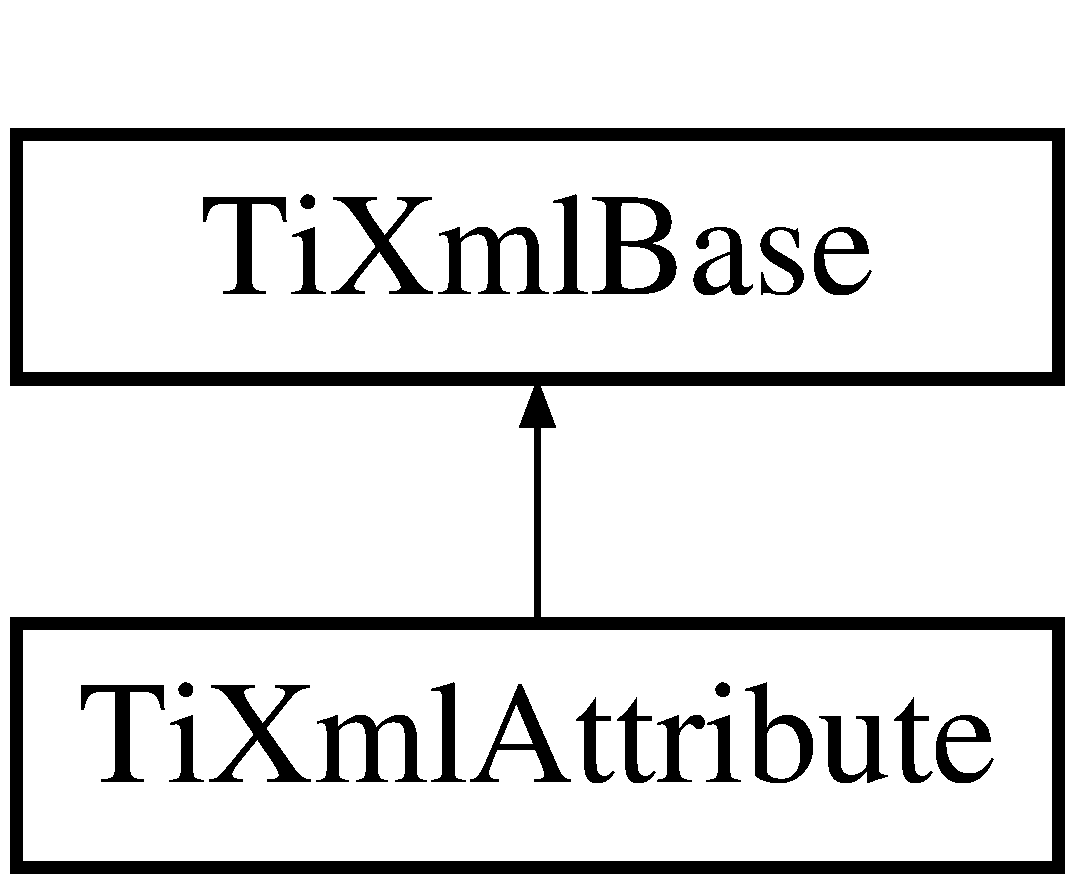
\includegraphics[height=2.000000cm]{class_ti_xml_attribute}
\end{center}
\end{figure}
\subsection*{\-Public \-Member \-Functions}
\begin{DoxyCompactItemize}
\item 
\hypertarget{class_ti_xml_attribute_a9cfa3c8179873fd485d83003b114f8e1}{
\hyperlink{class_ti_xml_attribute_a9cfa3c8179873fd485d83003b114f8e1}{\-Ti\-Xml\-Attribute} ()}
\label{class_ti_xml_attribute_a9cfa3c8179873fd485d83003b114f8e1}

\begin{DoxyCompactList}\small\item\em \-Construct an empty attribute. \end{DoxyCompactList}\item 
\hypertarget{class_ti_xml_attribute_a759d0b76fb8fcf765ecab243bc14f05e}{
\hyperlink{class_ti_xml_attribute_a759d0b76fb8fcf765ecab243bc14f05e}{\-Ti\-Xml\-Attribute} (const char $\ast$\-\_\-name, const char $\ast$\-\_\-value)}
\label{class_ti_xml_attribute_a759d0b76fb8fcf765ecab243bc14f05e}

\begin{DoxyCompactList}\small\item\em \-Construct an attribute with a name and value. \end{DoxyCompactList}\item 
const char $\ast$ \hyperlink{class_ti_xml_attribute_a298a57287d305904ba6bd96ae6f78d3d}{\-Name} () const 
\item 
const char $\ast$ \hyperlink{class_ti_xml_attribute_a0f874490eac8ca00ee0070765d0e97e3}{\-Value} () const 
\item 
\hypertarget{class_ti_xml_attribute_aa1a20ad59dc7e89a0ab265396360d50f}{
int \hyperlink{class_ti_xml_attribute_aa1a20ad59dc7e89a0ab265396360d50f}{\-Int\-Value} () const }
\label{class_ti_xml_attribute_aa1a20ad59dc7e89a0ab265396360d50f}

\begin{DoxyCompactList}\small\item\em \-Return the value of this attribute, converted to an integer. \end{DoxyCompactList}\item 
\hypertarget{class_ti_xml_attribute_a2880ddef53fc7522c99535273954d230}{
double \hyperlink{class_ti_xml_attribute_a2880ddef53fc7522c99535273954d230}{\-Double\-Value} () const }
\label{class_ti_xml_attribute_a2880ddef53fc7522c99535273954d230}

\begin{DoxyCompactList}\small\item\em \-Return the value of this attribute, converted to a double. \end{DoxyCompactList}\item 
\hypertarget{class_ti_xml_attribute_a64cee17bceb8232eb0736d26dd082d79}{
const \-T\-I\-X\-M\-L\-\_\-\-S\-T\-R\-I\-N\-G \& {\bfseries \-Name\-T\-Str} () const }
\label{class_ti_xml_attribute_a64cee17bceb8232eb0736d26dd082d79}

\item 
int \hyperlink{class_ti_xml_attribute_ad6c93088ee21af41a107931223339344}{\-Query\-Int\-Value} (int $\ast$\-\_\-value) const 
\item 
\hypertarget{class_ti_xml_attribute_ac87b2a8489906a5d7aa2875f20be3513}{
int \hyperlink{class_ti_xml_attribute_ac87b2a8489906a5d7aa2875f20be3513}{\-Query\-Double\-Value} (double $\ast$\-\_\-value) const }
\label{class_ti_xml_attribute_ac87b2a8489906a5d7aa2875f20be3513}

\begin{DoxyCompactList}\small\item\em \-Query\-Double\-Value examines the value string. \-See \hyperlink{class_ti_xml_attribute_ad6c93088ee21af41a107931223339344}{\-Query\-Int\-Value()}. \end{DoxyCompactList}\item 
void \hyperlink{class_ti_xml_attribute_ab7fa3d21ff8d7c5764cf9af15b667a99}{\-Set\-Name} (const char $\ast$\-\_\-name)
\item 
void \hyperlink{class_ti_xml_attribute_a2dae44178f668b3cb48101be4f2236a0}{\-Set\-Value} (const char $\ast$\-\_\-value)
\item 
\hypertarget{class_ti_xml_attribute_a7e065df640116a62ea4f4b7da5449cc8}{
void \hyperlink{class_ti_xml_attribute_a7e065df640116a62ea4f4b7da5449cc8}{\-Set\-Int\-Value} (int \-\_\-value)}
\label{class_ti_xml_attribute_a7e065df640116a62ea4f4b7da5449cc8}

\begin{DoxyCompactList}\small\item\em \-Set the value from an integer. \end{DoxyCompactList}\item 
\hypertarget{class_ti_xml_attribute_a0316da31373496c4368ad549bf711394}{
void \hyperlink{class_ti_xml_attribute_a0316da31373496c4368ad549bf711394}{\-Set\-Double\-Value} (double \-\_\-value)}
\label{class_ti_xml_attribute_a0316da31373496c4368ad549bf711394}

\begin{DoxyCompactList}\small\item\em \-Set the value from a double. \end{DoxyCompactList}\item 
\hypertarget{class_ti_xml_attribute_a776478980776a024f7c2846eec640f65}{
const \hyperlink{class_ti_xml_attribute}{\-Ti\-Xml\-Attribute} $\ast$ \hyperlink{class_ti_xml_attribute_a776478980776a024f7c2846eec640f65}{\-Next} () const }
\label{class_ti_xml_attribute_a776478980776a024f7c2846eec640f65}

\begin{DoxyCompactList}\small\item\em \-Get the next sibling attribute in the \-D\-O\-M. \-Returns null at end. \end{DoxyCompactList}\item 
\hypertarget{class_ti_xml_attribute_a138320aa7793b148ba7e5bd0a0ea4db6}{
\hyperlink{class_ti_xml_attribute}{\-Ti\-Xml\-Attribute} $\ast$ {\bfseries \-Next} ()}
\label{class_ti_xml_attribute_a138320aa7793b148ba7e5bd0a0ea4db6}

\item 
\hypertarget{class_ti_xml_attribute_a54a5f8730c7b02b9a41b74e12e27fe86}{
const \hyperlink{class_ti_xml_attribute}{\-Ti\-Xml\-Attribute} $\ast$ \hyperlink{class_ti_xml_attribute_a54a5f8730c7b02b9a41b74e12e27fe86}{\-Previous} () const }
\label{class_ti_xml_attribute_a54a5f8730c7b02b9a41b74e12e27fe86}

\begin{DoxyCompactList}\small\item\em \-Get the previous sibling attribute in the \-D\-O\-M. \-Returns null at beginning. \end{DoxyCompactList}\item 
\hypertarget{class_ti_xml_attribute_ae4dabc932cba945ed1e92fec5f121193}{
\hyperlink{class_ti_xml_attribute}{\-Ti\-Xml\-Attribute} $\ast$ {\bfseries \-Previous} ()}
\label{class_ti_xml_attribute_ae4dabc932cba945ed1e92fec5f121193}

\item 
\hypertarget{class_ti_xml_attribute_ae48c2a65b520d453914ce4e845d607cf}{
bool {\bfseries operator==} (const \hyperlink{class_ti_xml_attribute}{\-Ti\-Xml\-Attribute} \&rhs) const }
\label{class_ti_xml_attribute_ae48c2a65b520d453914ce4e845d607cf}

\item 
\hypertarget{class_ti_xml_attribute_adb8b6f2cad5948e73e383182e7ce10de}{
bool {\bfseries operator$<$} (const \hyperlink{class_ti_xml_attribute}{\-Ti\-Xml\-Attribute} \&rhs) const }
\label{class_ti_xml_attribute_adb8b6f2cad5948e73e383182e7ce10de}

\item 
\hypertarget{class_ti_xml_attribute_a867562769ef9778c1690cd373246b05b}{
bool {\bfseries operator$>$} (const \hyperlink{class_ti_xml_attribute}{\-Ti\-Xml\-Attribute} \&rhs) const }
\label{class_ti_xml_attribute_a867562769ef9778c1690cd373246b05b}

\item 
\hypertarget{class_ti_xml_attribute_ad62774421b814894b995af3b5d231dda}{
virtual const char $\ast$ {\bfseries \-Parse} (const char $\ast$p, \hyperlink{class_ti_xml_parsing_data}{\-Ti\-Xml\-Parsing\-Data} $\ast$data, \-Ti\-Xml\-Encoding encoding)}
\label{class_ti_xml_attribute_ad62774421b814894b995af3b5d231dda}

\item 
virtual void \hyperlink{class_ti_xml_attribute_acc04956c1d5c4c31fe74f7a7528d109a}{\-Print} (\-F\-I\-L\-E $\ast$cfile, int depth) const 
\item 
\hypertarget{class_ti_xml_attribute_a19e6b6862a80b188571c47947e88d030}{
void {\bfseries \-Print} (\-F\-I\-L\-E $\ast$cfile, int depth, \-T\-I\-X\-M\-L\-\_\-\-S\-T\-R\-I\-N\-G $\ast$str) const }
\label{class_ti_xml_attribute_a19e6b6862a80b188571c47947e88d030}

\item 
\hypertarget{class_ti_xml_attribute_ac12a94d4548302afb12f488ba101f7d1}{
void {\bfseries \-Set\-Document} (\hyperlink{class_ti_xml_document}{\-Ti\-Xml\-Document} $\ast$doc)}
\label{class_ti_xml_attribute_ac12a94d4548302afb12f488ba101f7d1}

\end{DoxyCompactItemize}
\subsection*{\-Friends}
\begin{DoxyCompactItemize}
\item 
\hypertarget{class_ti_xml_attribute_a35a7b7f89f708527677d5078d41ce0bf}{
class {\bfseries \-Ti\-Xml\-Attribute\-Set}}
\label{class_ti_xml_attribute_a35a7b7f89f708527677d5078d41ce0bf}

\end{DoxyCompactItemize}


\subsection{\-Detailed \-Description}
\-An attribute is a name-\/value pair. \-Elements have an arbitrary number of attributes, each with a unique name.

\begin{DoxyNote}{\-Note}
\-The attributes are not \-Ti\-Xml\-Nodes, since they are not part of the tiny\-X\-M\-L document object model. \-There are other suggested ways to look at this problem. 
\end{DoxyNote}


\subsection{\-Member \-Function \-Documentation}
\hypertarget{class_ti_xml_attribute_a298a57287d305904ba6bd96ae6f78d3d}{
\index{\-Ti\-Xml\-Attribute@{\-Ti\-Xml\-Attribute}!\-Name@{\-Name}}
\index{\-Name@{\-Name}!TiXmlAttribute@{\-Ti\-Xml\-Attribute}}
\subsubsection[{\-Name}]{\setlength{\rightskip}{0pt plus 5cm}const char$\ast$ \-Ti\-Xml\-Attribute\-::\-Name (
\begin{DoxyParamCaption}
{}
\end{DoxyParamCaption}
) const\hspace{0.3cm}{\ttfamily  \mbox{[}inline\mbox{]}}}}
\label{class_ti_xml_attribute_a298a57287d305904ba6bd96ae6f78d3d}
$<$ \-Return the name of this attribute. \hypertarget{class_ti_xml_attribute_acc04956c1d5c4c31fe74f7a7528d109a}{
\index{\-Ti\-Xml\-Attribute@{\-Ti\-Xml\-Attribute}!\-Print@{\-Print}}
\index{\-Print@{\-Print}!TiXmlAttribute@{\-Ti\-Xml\-Attribute}}
\subsubsection[{\-Print}]{\setlength{\rightskip}{0pt plus 5cm}virtual void \-Ti\-Xml\-Attribute\-::\-Print (
\begin{DoxyParamCaption}
\item[{\-F\-I\-L\-E $\ast$}]{cfile, }
\item[{int}]{depth}
\end{DoxyParamCaption}
) const\hspace{0.3cm}{\ttfamily  \mbox{[}inline, virtual\mbox{]}}}}
\label{class_ti_xml_attribute_acc04956c1d5c4c31fe74f7a7528d109a}
\-All \-Tiny\-Xml classes can print themselves to a filestream or the string class (\hyperlink{class_ti_xml_string}{\-Ti\-Xml\-String} in non-\/\-S\-T\-L mode, std\-::string in \-S\-T\-L mode.) \-Either or both cfile and str can be null.

\-This is a formatted print, and will insert tabs and newlines.

(\-For an unformatted stream, use the $<$$<$ operator.) 

\-Implements \hyperlink{class_ti_xml_base_a0de56b3f2ef14c65091a3b916437b512}{\-Ti\-Xml\-Base}.

\hypertarget{class_ti_xml_attribute_ad6c93088ee21af41a107931223339344}{
\index{\-Ti\-Xml\-Attribute@{\-Ti\-Xml\-Attribute}!\-Query\-Int\-Value@{\-Query\-Int\-Value}}
\index{\-Query\-Int\-Value@{\-Query\-Int\-Value}!TiXmlAttribute@{\-Ti\-Xml\-Attribute}}
\subsubsection[{\-Query\-Int\-Value}]{\setlength{\rightskip}{0pt plus 5cm}int \-Ti\-Xml\-Attribute\-::\-Query\-Int\-Value (
\begin{DoxyParamCaption}
\item[{int $\ast$}]{\-\_\-value}
\end{DoxyParamCaption}
) const}}
\label{class_ti_xml_attribute_ad6c93088ee21af41a107931223339344}
\-Query\-Int\-Value examines the value string. \-It is an alternative to the \hyperlink{class_ti_xml_attribute_aa1a20ad59dc7e89a0ab265396360d50f}{\-Int\-Value()} method with richer error checking. \-If the value is an integer, it is stored in 'value' and the call returns \-T\-I\-X\-M\-L\-\_\-\-S\-U\-C\-C\-E\-S\-S. \-If it is not an integer, it returns \-T\-I\-X\-M\-L\-\_\-\-W\-R\-O\-N\-G\-\_\-\-T\-Y\-P\-E.

\-A specialized but useful call. \-Note that for success it returns 0, which is the opposite of almost all other \-Tiny\-Xml calls. \hypertarget{class_ti_xml_attribute_ab7fa3d21ff8d7c5764cf9af15b667a99}{
\index{\-Ti\-Xml\-Attribute@{\-Ti\-Xml\-Attribute}!\-Set\-Name@{\-Set\-Name}}
\index{\-Set\-Name@{\-Set\-Name}!TiXmlAttribute@{\-Ti\-Xml\-Attribute}}
\subsubsection[{\-Set\-Name}]{\setlength{\rightskip}{0pt plus 5cm}void \-Ti\-Xml\-Attribute\-::\-Set\-Name (
\begin{DoxyParamCaption}
\item[{const char $\ast$}]{\-\_\-name}
\end{DoxyParamCaption}
)\hspace{0.3cm}{\ttfamily  \mbox{[}inline\mbox{]}}}}
\label{class_ti_xml_attribute_ab7fa3d21ff8d7c5764cf9af15b667a99}
$<$ \-Set the name of this attribute. \hypertarget{class_ti_xml_attribute_a2dae44178f668b3cb48101be4f2236a0}{
\index{\-Ti\-Xml\-Attribute@{\-Ti\-Xml\-Attribute}!\-Set\-Value@{\-Set\-Value}}
\index{\-Set\-Value@{\-Set\-Value}!TiXmlAttribute@{\-Ti\-Xml\-Attribute}}
\subsubsection[{\-Set\-Value}]{\setlength{\rightskip}{0pt plus 5cm}void \-Ti\-Xml\-Attribute\-::\-Set\-Value (
\begin{DoxyParamCaption}
\item[{const char $\ast$}]{\-\_\-value}
\end{DoxyParamCaption}
)\hspace{0.3cm}{\ttfamily  \mbox{[}inline\mbox{]}}}}
\label{class_ti_xml_attribute_a2dae44178f668b3cb48101be4f2236a0}
$<$ \-Set the value. \hypertarget{class_ti_xml_attribute_a0f874490eac8ca00ee0070765d0e97e3}{
\index{\-Ti\-Xml\-Attribute@{\-Ti\-Xml\-Attribute}!\-Value@{\-Value}}
\index{\-Value@{\-Value}!TiXmlAttribute@{\-Ti\-Xml\-Attribute}}
\subsubsection[{\-Value}]{\setlength{\rightskip}{0pt plus 5cm}const char$\ast$ \-Ti\-Xml\-Attribute\-::\-Value (
\begin{DoxyParamCaption}
{}
\end{DoxyParamCaption}
) const\hspace{0.3cm}{\ttfamily  \mbox{[}inline\mbox{]}}}}
\label{class_ti_xml_attribute_a0f874490eac8ca00ee0070765d0e97e3}
$<$ \-Return the value of this attribute. 

\-The documentation for this class was generated from the following files\-:\begin{DoxyCompactItemize}
\item 
/home/cshome/m/mabrams/345/txt\-Engine/tinyxml.\-h\item 
/home/cshome/m/mabrams/345/txt\-Engine/tinyxml.\-cpp\item 
/home/cshome/m/mabrams/345/txt\-Engine/tinyxmlparser.\-cpp\end{DoxyCompactItemize}

\hypertarget{class_ti_xml_attribute_set}{
\section{TiXmlAttributeSet Class Reference}
\label{class_ti_xml_attribute_set}\index{TiXmlAttributeSet@{TiXmlAttributeSet}}
}
\subsection*{Public Member Functions}
\begin{DoxyCompactItemize}
\item 
\hypertarget{class_ti_xml_attribute_set_a745e50ddaae3bee93e4589321e0b9c1a}{
void {\bfseries Add} (\hyperlink{class_ti_xml_attribute}{TiXmlAttribute} $\ast$attribute)}
\label{class_ti_xml_attribute_set_a745e50ddaae3bee93e4589321e0b9c1a}

\item 
\hypertarget{class_ti_xml_attribute_set_a924a73d071f2573f9060f0be57879c57}{
void {\bfseries Remove} (\hyperlink{class_ti_xml_attribute}{TiXmlAttribute} $\ast$attribute)}
\label{class_ti_xml_attribute_set_a924a73d071f2573f9060f0be57879c57}

\item 
\hypertarget{class_ti_xml_attribute_set_ae0636e88cedd4b09d61c451860f68598}{
const \hyperlink{class_ti_xml_attribute}{TiXmlAttribute} $\ast$ {\bfseries First} () const }
\label{class_ti_xml_attribute_set_ae0636e88cedd4b09d61c451860f68598}

\item 
\hypertarget{class_ti_xml_attribute_set_a99703bb08ca2aece2d7ef835de339ba0}{
\hyperlink{class_ti_xml_attribute}{TiXmlAttribute} $\ast$ {\bfseries First} ()}
\label{class_ti_xml_attribute_set_a99703bb08ca2aece2d7ef835de339ba0}

\item 
\hypertarget{class_ti_xml_attribute_set_a7b3f3ccf39a97bc25539d3fcc540296a}{
const \hyperlink{class_ti_xml_attribute}{TiXmlAttribute} $\ast$ {\bfseries Last} () const }
\label{class_ti_xml_attribute_set_a7b3f3ccf39a97bc25539d3fcc540296a}

\item 
\hypertarget{class_ti_xml_attribute_set_ab4c4edfb2d74f6ea31aae096743bd6e0}{
\hyperlink{class_ti_xml_attribute}{TiXmlAttribute} $\ast$ {\bfseries Last} ()}
\label{class_ti_xml_attribute_set_ab4c4edfb2d74f6ea31aae096743bd6e0}

\item 
\hypertarget{class_ti_xml_attribute_set_af3675cc2bfd0aea153cda1cfcdd1f77e}{
\hyperlink{class_ti_xml_attribute}{TiXmlAttribute} $\ast$ {\bfseries Find} (const char $\ast$\_\-name) const }
\label{class_ti_xml_attribute_set_af3675cc2bfd0aea153cda1cfcdd1f77e}

\item 
\hypertarget{class_ti_xml_attribute_set_a5e28f5d32f048fba85d04dc317495bdc}{
\hyperlink{class_ti_xml_attribute}{TiXmlAttribute} $\ast$ {\bfseries FindOrCreate} (const char $\ast$\_\-name)}
\label{class_ti_xml_attribute_set_a5e28f5d32f048fba85d04dc317495bdc}

\end{DoxyCompactItemize}


The documentation for this class was generated from the following files:\begin{DoxyCompactItemize}
\item 
/home/cshome/m/mabrams/345/txtEngine/tinyxml.h\item 
/home/cshome/m/mabrams/345/txtEngine/tinyxml.cpp\end{DoxyCompactItemize}

\hypertarget{class_ti_xml_base}{
\section{\-Ti\-Xml\-Base \-Class \-Reference}
\label{class_ti_xml_base}\index{\-Ti\-Xml\-Base@{\-Ti\-Xml\-Base}}
}


{\ttfamily \#include $<$tinyxml.\-h$>$}

\-Inheritance diagram for \-Ti\-Xml\-Base\-:\begin{figure}[H]
\begin{center}
\leavevmode
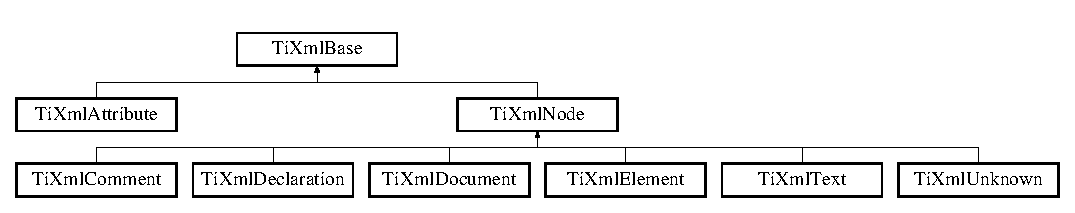
\includegraphics[height=2.413793cm]{class_ti_xml_base}
\end{center}
\end{figure}
\subsection*{\-Classes}
\begin{DoxyCompactItemize}
\item 
struct {\bfseries \-Entity}
\end{DoxyCompactItemize}
\subsection*{\-Public \-Types}
\begin{DoxyCompactItemize}
\item 
enum \{ \*
{\bfseries \-T\-I\-X\-M\-L\-\_\-\-N\-O\-\_\-\-E\-R\-R\-O\-R} =  0, 
{\bfseries \-T\-I\-X\-M\-L\-\_\-\-E\-R\-R\-O\-R}, 
{\bfseries \-T\-I\-X\-M\-L\-\_\-\-E\-R\-R\-O\-R\-\_\-\-O\-P\-E\-N\-I\-N\-G\-\_\-\-F\-I\-L\-E}, 
{\bfseries \-T\-I\-X\-M\-L\-\_\-\-E\-R\-R\-O\-R\-\_\-\-P\-A\-R\-S\-I\-N\-G\-\_\-\-E\-L\-E\-M\-E\-N\-T}, 
\*
{\bfseries \-T\-I\-X\-M\-L\-\_\-\-E\-R\-R\-O\-R\-\_\-\-F\-A\-I\-L\-E\-D\-\_\-\-T\-O\-\_\-\-R\-E\-A\-D\-\_\-\-E\-L\-E\-M\-E\-N\-T\-\_\-\-N\-A\-M\-E}, 
{\bfseries \-T\-I\-X\-M\-L\-\_\-\-E\-R\-R\-O\-R\-\_\-\-R\-E\-A\-D\-I\-N\-G\-\_\-\-E\-L\-E\-M\-E\-N\-T\-\_\-\-V\-A\-L\-U\-E}, 
{\bfseries \-T\-I\-X\-M\-L\-\_\-\-E\-R\-R\-O\-R\-\_\-\-R\-E\-A\-D\-I\-N\-G\-\_\-\-A\-T\-T\-R\-I\-B\-U\-T\-E\-S}, 
{\bfseries \-T\-I\-X\-M\-L\-\_\-\-E\-R\-R\-O\-R\-\_\-\-P\-A\-R\-S\-I\-N\-G\-\_\-\-E\-M\-P\-T\-Y}, 
\*
{\bfseries \-T\-I\-X\-M\-L\-\_\-\-E\-R\-R\-O\-R\-\_\-\-R\-E\-A\-D\-I\-N\-G\-\_\-\-E\-N\-D\-\_\-\-T\-A\-G}, 
{\bfseries \-T\-I\-X\-M\-L\-\_\-\-E\-R\-R\-O\-R\-\_\-\-P\-A\-R\-S\-I\-N\-G\-\_\-\-U\-N\-K\-N\-O\-W\-N}, 
{\bfseries \-T\-I\-X\-M\-L\-\_\-\-E\-R\-R\-O\-R\-\_\-\-P\-A\-R\-S\-I\-N\-G\-\_\-\-C\-O\-M\-M\-E\-N\-T}, 
{\bfseries \-T\-I\-X\-M\-L\-\_\-\-E\-R\-R\-O\-R\-\_\-\-P\-A\-R\-S\-I\-N\-G\-\_\-\-D\-E\-C\-L\-A\-R\-A\-T\-I\-O\-N}, 
\*
{\bfseries \-T\-I\-X\-M\-L\-\_\-\-E\-R\-R\-O\-R\-\_\-\-D\-O\-C\-U\-M\-E\-N\-T\-\_\-\-E\-M\-P\-T\-Y}, 
{\bfseries \-T\-I\-X\-M\-L\-\_\-\-E\-R\-R\-O\-R\-\_\-\-E\-M\-B\-E\-D\-D\-E\-D\-\_\-\-N\-U\-L\-L}, 
{\bfseries \-T\-I\-X\-M\-L\-\_\-\-E\-R\-R\-O\-R\-\_\-\-P\-A\-R\-S\-I\-N\-G\-\_\-\-C\-D\-A\-T\-A}, 
{\bfseries \-T\-I\-X\-M\-L\-\_\-\-E\-R\-R\-O\-R\-\_\-\-D\-O\-C\-U\-M\-E\-N\-T\-\_\-\-T\-O\-P\-\_\-\-O\-N\-L\-Y}, 
\*
{\bfseries \-T\-I\-X\-M\-L\-\_\-\-E\-R\-R\-O\-R\-\_\-\-S\-T\-R\-I\-N\-G\-\_\-\-C\-O\-U\-N\-T}
 \}
\end{DoxyCompactItemize}
\subsection*{\-Public \-Member \-Functions}
\begin{DoxyCompactItemize}
\item 
virtual void \hyperlink{class_ti_xml_base_a0de56b3f2ef14c65091a3b916437b512}{\-Print} (\-F\-I\-L\-E $\ast$cfile, int depth) const =0
\item 
int \hyperlink{class_ti_xml_base_a024bceb070188df92c2a8d8852dd0853}{\-Row} () const 
\item 
int \hyperlink{class_ti_xml_base_ab54bfb9b70fe6dd276e7b279cab7f003}{\-Column} () const 
\item 
void \hyperlink{class_ti_xml_base_ac6b3e0f790930d4970ec30764e937b5d}{\-Set\-User\-Data} (void $\ast$user)
\item 
void $\ast$ \hyperlink{class_ti_xml_base_a6559a530ca6763fc301a14d77ed28c17}{\-Get\-User\-Data} ()
\item 
const void $\ast$ \hyperlink{class_ti_xml_base_ad0120210e4680ef2088601753ce0ede4}{\-Get\-User\-Data} () const 
\item 
\hypertarget{class_ti_xml_base_a00e4edb0219d00a1379c856e5a1d2025}{
virtual const char $\ast$ {\bfseries \-Parse} (const char $\ast$p, \hyperlink{class_ti_xml_parsing_data}{\-Ti\-Xml\-Parsing\-Data} $\ast$data, \-Ti\-Xml\-Encoding encoding)=0}
\label{class_ti_xml_base_a00e4edb0219d00a1379c856e5a1d2025}

\end{DoxyCompactItemize}
\subsection*{\-Static \-Public \-Member \-Functions}
\begin{DoxyCompactItemize}
\item 
static void \hyperlink{class_ti_xml_base_a0f799ec645bfb8d8a969e83478f379c1}{\-Set\-Condense\-White\-Space} (bool condense)
\item 
\hypertarget{class_ti_xml_base_ad4b1472531c647a25b1840a87ae42438}{
static bool \hyperlink{class_ti_xml_base_ad4b1472531c647a25b1840a87ae42438}{\-Is\-White\-Space\-Condensed} ()}
\label{class_ti_xml_base_ad4b1472531c647a25b1840a87ae42438}

\begin{DoxyCompactList}\small\item\em \-Return the current white space setting. \end{DoxyCompactList}\item 
static void \hyperlink{class_ti_xml_base_a32ed202562b58de64c7d799ca3c9db98}{\-Encode\-String} (const \-T\-I\-X\-M\-L\-\_\-\-S\-T\-R\-I\-N\-G \&str, \-T\-I\-X\-M\-L\-\_\-\-S\-T\-R\-I\-N\-G $\ast$out)
\end{DoxyCompactItemize}
\subsection*{\-Static \-Public \-Attributes}
\begin{DoxyCompactItemize}
\item 
static const int {\bfseries utf8\-Byte\-Table} \mbox{[}256\mbox{]}
\end{DoxyCompactItemize}
\subsection*{\-Static \-Protected \-Member \-Functions}
\begin{DoxyCompactItemize}
\item 
\hypertarget{class_ti_xml_base_ac0c3d66d8a9e6996a1fa016275e16875}{
static const char $\ast$ {\bfseries \-Skip\-White\-Space} (const char $\ast$, \-Ti\-Xml\-Encoding encoding)}
\label{class_ti_xml_base_ac0c3d66d8a9e6996a1fa016275e16875}

\item 
\hypertarget{class_ti_xml_base_af56296d561c0bab4bc8e198cdcf5c48e}{
static bool {\bfseries \-Is\-White\-Space} (char c)}
\label{class_ti_xml_base_af56296d561c0bab4bc8e198cdcf5c48e}

\item 
\hypertarget{class_ti_xml_base_a3de391ea9f4c4a8aa10d04480b048795}{
static bool {\bfseries \-Is\-White\-Space} (int c)}
\label{class_ti_xml_base_a3de391ea9f4c4a8aa10d04480b048795}

\item 
\hypertarget{class_ti_xml_base_a1c21a6ab5f7b503acd91f35f183734b3}{
static const char $\ast$ {\bfseries \-Read\-Name} (const char $\ast$p, \-T\-I\-X\-M\-L\-\_\-\-S\-T\-R\-I\-N\-G $\ast$name, \-Ti\-Xml\-Encoding encoding)}
\label{class_ti_xml_base_a1c21a6ab5f7b503acd91f35f183734b3}

\item 
\hypertarget{class_ti_xml_base_aa646c74921aa33156968b802bbf5566e}{
static const char $\ast$ {\bfseries \-Read\-Text} (const char $\ast$in, \-T\-I\-X\-M\-L\-\_\-\-S\-T\-R\-I\-N\-G $\ast$text, bool ignore\-White\-Space, const char $\ast$end\-Tag, bool ignore\-Case, \-Ti\-Xml\-Encoding encoding)}
\label{class_ti_xml_base_aa646c74921aa33156968b802bbf5566e}

\item 
\hypertarget{class_ti_xml_base_ac5c08bf3deffcda0bf8ce2958372b584}{
static const char $\ast$ {\bfseries \-Get\-Entity} (const char $\ast$in, char $\ast$value, int $\ast$length, \-Ti\-Xml\-Encoding encoding)}
\label{class_ti_xml_base_ac5c08bf3deffcda0bf8ce2958372b584}

\item 
\hypertarget{class_ti_xml_base_a5b0fde72d6f662ae1fd6303195d2159b}{
static const char $\ast$ {\bfseries \-Get\-Char} (const char $\ast$p, char $\ast$\-\_\-value, int $\ast$length, \-Ti\-Xml\-Encoding encoding)}
\label{class_ti_xml_base_a5b0fde72d6f662ae1fd6303195d2159b}

\item 
\hypertarget{class_ti_xml_base_a51631e6986179558b9e5850723ed165a}{
static bool {\bfseries \-String\-Equal} (const char $\ast$p, const char $\ast$end\-Tag, bool ignore\-Case, \-Ti\-Xml\-Encoding encoding)}
\label{class_ti_xml_base_a51631e6986179558b9e5850723ed165a}

\item 
\hypertarget{class_ti_xml_base_ae22522b2e8e1ac43102d16394f639fc8}{
static int {\bfseries \-Is\-Alpha} (unsigned char any\-Byte, \-Ti\-Xml\-Encoding encoding)}
\label{class_ti_xml_base_ae22522b2e8e1ac43102d16394f639fc8}

\item 
\hypertarget{class_ti_xml_base_a321919055c115c78ded17f85a793f368}{
static int {\bfseries \-Is\-Alpha\-Num} (unsigned char any\-Byte, \-Ti\-Xml\-Encoding encoding)}
\label{class_ti_xml_base_a321919055c115c78ded17f85a793f368}

\item 
\hypertarget{class_ti_xml_base_a799f17405a86a5c2029618e85f11a097}{
static int {\bfseries \-To\-Lower} (int v, \-Ti\-Xml\-Encoding encoding)}
\label{class_ti_xml_base_a799f17405a86a5c2029618e85f11a097}

\item 
\hypertarget{class_ti_xml_base_a07c765e3a7f979d343e646ea797b180b}{
static void {\bfseries \-Convert\-U\-T\-F32\-To\-U\-T\-F8} (unsigned long input, char $\ast$output, int $\ast$length)}
\label{class_ti_xml_base_a07c765e3a7f979d343e646ea797b180b}

\end{DoxyCompactItemize}
\subsection*{\-Protected \-Attributes}
\begin{DoxyCompactItemize}
\item 
\hypertarget{class_ti_xml_base_a0d992580f3bc264909f898e942677a3c}{
\hyperlink{struct_ti_xml_cursor}{\-Ti\-Xml\-Cursor} {\bfseries location}}
\label{class_ti_xml_base_a0d992580f3bc264909f898e942677a3c}

\item 
\hypertarget{class_ti_xml_base_ab242c01590191f644569fa89a080d97c}{
void $\ast$ \hyperlink{class_ti_xml_base_ab242c01590191f644569fa89a080d97c}{user\-Data}}
\label{class_ti_xml_base_ab242c01590191f644569fa89a080d97c}

\begin{DoxyCompactList}\small\item\em \-Field containing a generic user pointer. \end{DoxyCompactList}\end{DoxyCompactItemize}
\subsection*{\-Static \-Protected \-Attributes}
\begin{DoxyCompactItemize}
\item 
static const char $\ast$ {\bfseries error\-String} \mbox{[}\-T\-I\-X\-M\-L\-\_\-\-E\-R\-R\-O\-R\-\_\-\-S\-T\-R\-I\-N\-G\-\_\-\-C\-O\-U\-N\-T\mbox{]}
\end{DoxyCompactItemize}
\subsection*{\-Friends}
\begin{DoxyCompactItemize}
\item 
\hypertarget{class_ti_xml_base_a218872a0d985ae30e78c55adc4bdb196}{
class {\bfseries \-Ti\-Xml\-Node}}
\label{class_ti_xml_base_a218872a0d985ae30e78c55adc4bdb196}

\item 
\hypertarget{class_ti_xml_base_ab6592e32cb9132be517cc12a70564c4b}{
class {\bfseries \-Ti\-Xml\-Element}}
\label{class_ti_xml_base_ab6592e32cb9132be517cc12a70564c4b}

\item 
\hypertarget{class_ti_xml_base_a173617f6dfe902cf484ce5552b950475}{
class {\bfseries \-Ti\-Xml\-Document}}
\label{class_ti_xml_base_a173617f6dfe902cf484ce5552b950475}

\end{DoxyCompactItemize}


\subsection{\-Detailed \-Description}
\hyperlink{class_ti_xml_base}{\-Ti\-Xml\-Base} is a base class for every class in \-Tiny\-Xml. \-It does little except to establish that \-Tiny\-Xml classes can be printed and provide some utility functions.

\-In \-X\-M\-L, the document and elements can contain other elements and other types of nodes.

\begin{DoxyVerb}
	A Document can contain:	Element	(container or leaf)
							Comment (leaf)
							Unknown (leaf)
							Declaration( leaf )

	An Element can contain:	Element (container or leaf)
							Text	(leaf)
							Attributes (not on tree)
							Comment (leaf)
							Unknown (leaf)

	A Decleration contains: Attributes (not on tree)
	\end{DoxyVerb}
 

\subsection{\-Member \-Function \-Documentation}
\hypertarget{class_ti_xml_base_ab54bfb9b70fe6dd276e7b279cab7f003}{
\index{\-Ti\-Xml\-Base@{\-Ti\-Xml\-Base}!\-Column@{\-Column}}
\index{\-Column@{\-Column}!TiXmlBase@{\-Ti\-Xml\-Base}}
\subsubsection[{\-Column}]{\setlength{\rightskip}{0pt plus 5cm}int \-Ti\-Xml\-Base\-::\-Column (
\begin{DoxyParamCaption}
{}
\end{DoxyParamCaption}
) const\hspace{0.3cm}{\ttfamily  \mbox{[}inline\mbox{]}}}}
\label{class_ti_xml_base_ab54bfb9b70fe6dd276e7b279cab7f003}
$<$ \-See \hyperlink{class_ti_xml_base_a024bceb070188df92c2a8d8852dd0853}{\-Row()} \hypertarget{class_ti_xml_base_a32ed202562b58de64c7d799ca3c9db98}{
\index{\-Ti\-Xml\-Base@{\-Ti\-Xml\-Base}!\-Encode\-String@{\-Encode\-String}}
\index{\-Encode\-String@{\-Encode\-String}!TiXmlBase@{\-Ti\-Xml\-Base}}
\subsubsection[{\-Encode\-String}]{\setlength{\rightskip}{0pt plus 5cm}void \-Ti\-Xml\-Base\-::\-Encode\-String (
\begin{DoxyParamCaption}
\item[{const \-T\-I\-X\-M\-L\-\_\-\-S\-T\-R\-I\-N\-G \&}]{str, }
\item[{\-T\-I\-X\-M\-L\-\_\-\-S\-T\-R\-I\-N\-G $\ast$}]{out}
\end{DoxyParamCaption}
)\hspace{0.3cm}{\ttfamily  \mbox{[}static\mbox{]}}}}
\label{class_ti_xml_base_a32ed202562b58de64c7d799ca3c9db98}
\-Expands entities in a string. \-Note this should not contian the tag's '$<$', '$>$', etc, or they will be transformed into entities! \hypertarget{class_ti_xml_base_a6559a530ca6763fc301a14d77ed28c17}{
\index{\-Ti\-Xml\-Base@{\-Ti\-Xml\-Base}!\-Get\-User\-Data@{\-Get\-User\-Data}}
\index{\-Get\-User\-Data@{\-Get\-User\-Data}!TiXmlBase@{\-Ti\-Xml\-Base}}
\subsubsection[{\-Get\-User\-Data}]{\setlength{\rightskip}{0pt plus 5cm}void$\ast$ \-Ti\-Xml\-Base\-::\-Get\-User\-Data (
\begin{DoxyParamCaption}
{}
\end{DoxyParamCaption}
)\hspace{0.3cm}{\ttfamily  \mbox{[}inline\mbox{]}}}}
\label{class_ti_xml_base_a6559a530ca6763fc301a14d77ed28c17}
$<$ \-Get a pointer to arbitrary user data. \hypertarget{class_ti_xml_base_ad0120210e4680ef2088601753ce0ede4}{
\index{\-Ti\-Xml\-Base@{\-Ti\-Xml\-Base}!\-Get\-User\-Data@{\-Get\-User\-Data}}
\index{\-Get\-User\-Data@{\-Get\-User\-Data}!TiXmlBase@{\-Ti\-Xml\-Base}}
\subsubsection[{\-Get\-User\-Data}]{\setlength{\rightskip}{0pt plus 5cm}const void$\ast$ \-Ti\-Xml\-Base\-::\-Get\-User\-Data (
\begin{DoxyParamCaption}
{}
\end{DoxyParamCaption}
) const\hspace{0.3cm}{\ttfamily  \mbox{[}inline\mbox{]}}}}
\label{class_ti_xml_base_ad0120210e4680ef2088601753ce0ede4}
$<$ \-Get a pointer to arbitrary user data. \hypertarget{class_ti_xml_base_a0de56b3f2ef14c65091a3b916437b512}{
\index{\-Ti\-Xml\-Base@{\-Ti\-Xml\-Base}!\-Print@{\-Print}}
\index{\-Print@{\-Print}!TiXmlBase@{\-Ti\-Xml\-Base}}
\subsubsection[{\-Print}]{\setlength{\rightskip}{0pt plus 5cm}virtual void \-Ti\-Xml\-Base\-::\-Print (
\begin{DoxyParamCaption}
\item[{\-F\-I\-L\-E $\ast$}]{cfile, }
\item[{int}]{depth}
\end{DoxyParamCaption}
) const\hspace{0.3cm}{\ttfamily  \mbox{[}pure virtual\mbox{]}}}}
\label{class_ti_xml_base_a0de56b3f2ef14c65091a3b916437b512}
\-All \-Tiny\-Xml classes can print themselves to a filestream or the string class (\hyperlink{class_ti_xml_string}{\-Ti\-Xml\-String} in non-\/\-S\-T\-L mode, std\-::string in \-S\-T\-L mode.) \-Either or both cfile and str can be null.

\-This is a formatted print, and will insert tabs and newlines.

(\-For an unformatted stream, use the $<$$<$ operator.) 

\-Implemented in \hyperlink{class_ti_xml_document_a7b1aea204fee266b70b9c105c8bf2ada}{\-Ti\-Xml\-Document}, \hyperlink{class_ti_xml_unknown_a025f19c21ef01ea9be50febb8fe0ba06}{\-Ti\-Xml\-Unknown}, \hyperlink{class_ti_xml_declaration_abf6303db4bd05b5be554036817ff1cb4}{\-Ti\-Xml\-Declaration}, \hyperlink{class_ti_xml_text_ae74d56c5b3ddec6cc3103dd51821af92}{\-Ti\-Xml\-Text}, \hyperlink{class_ti_xml_comment_a17398061d62c470f57801ce28fa33ad4}{\-Ti\-Xml\-Comment}, \hyperlink{class_ti_xml_element_ad9d0c008866982ab8d9aafae7e14d692}{\-Ti\-Xml\-Element}, and \hyperlink{class_ti_xml_attribute_acc04956c1d5c4c31fe74f7a7528d109a}{\-Ti\-Xml\-Attribute}.

\hypertarget{class_ti_xml_base_a024bceb070188df92c2a8d8852dd0853}{
\index{\-Ti\-Xml\-Base@{\-Ti\-Xml\-Base}!\-Row@{\-Row}}
\index{\-Row@{\-Row}!TiXmlBase@{\-Ti\-Xml\-Base}}
\subsubsection[{\-Row}]{\setlength{\rightskip}{0pt plus 5cm}int \-Ti\-Xml\-Base\-::\-Row (
\begin{DoxyParamCaption}
{}
\end{DoxyParamCaption}
) const\hspace{0.3cm}{\ttfamily  \mbox{[}inline\mbox{]}}}}
\label{class_ti_xml_base_a024bceb070188df92c2a8d8852dd0853}
\-Return the position, in the original source file, of this node or attribute. \-The row and column are 1-\/based. (\-That is the first row and first column is 1,1). \-If the returns values are 0 or less, then the parser does not have a row and column value.

\-Generally, the row and column value will be set when the \-Ti\-Xml\-Document\-::\-Load(), \hyperlink{class_ti_xml_document_a4c852a889c02cf251117fd1d9fe1845f}{\-Ti\-Xml\-Document\-::\-Load\-File()}, or any \-Ti\-Xml\-Node\-::\-Parse() is called. \-It will \-N\-O\-T be set when the \-D\-O\-M was created from operator$>$$>$.

\-The values reflect the initial load. \-Once the \-D\-O\-M is modified programmatically (by adding or changing nodes and attributes) the new values will \-N\-O\-T update to reflect changes in the document.

\-There is a minor performance cost to computing the row and column. \-Computation can be disabled if \hyperlink{class_ti_xml_document_a51dac56316f89b35bdb7d0d433ba988e}{\-Ti\-Xml\-Document\-::\-Set\-Tab\-Size()} is called with 0 as the value.

\begin{DoxySeeAlso}{\-See also}
\hyperlink{class_ti_xml_document_a51dac56316f89b35bdb7d0d433ba988e}{\-Ti\-Xml\-Document\-::\-Set\-Tab\-Size()} 
\end{DoxySeeAlso}
\hypertarget{class_ti_xml_base_a0f799ec645bfb8d8a969e83478f379c1}{
\index{\-Ti\-Xml\-Base@{\-Ti\-Xml\-Base}!\-Set\-Condense\-White\-Space@{\-Set\-Condense\-White\-Space}}
\index{\-Set\-Condense\-White\-Space@{\-Set\-Condense\-White\-Space}!TiXmlBase@{\-Ti\-Xml\-Base}}
\subsubsection[{\-Set\-Condense\-White\-Space}]{\setlength{\rightskip}{0pt plus 5cm}static void \-Ti\-Xml\-Base\-::\-Set\-Condense\-White\-Space (
\begin{DoxyParamCaption}
\item[{bool}]{condense}
\end{DoxyParamCaption}
)\hspace{0.3cm}{\ttfamily  \mbox{[}inline, static\mbox{]}}}}
\label{class_ti_xml_base_a0f799ec645bfb8d8a969e83478f379c1}
\-The world does not agree on whether white space should be kept or not. \-In order to make everyone happy, these global, static functions are provided to set whether or not \-Tiny\-Xml will condense all white space into a single space or not. \-The default is to condense. \-Note changing this value is not thread safe. \hypertarget{class_ti_xml_base_ac6b3e0f790930d4970ec30764e937b5d}{
\index{\-Ti\-Xml\-Base@{\-Ti\-Xml\-Base}!\-Set\-User\-Data@{\-Set\-User\-Data}}
\index{\-Set\-User\-Data@{\-Set\-User\-Data}!TiXmlBase@{\-Ti\-Xml\-Base}}
\subsubsection[{\-Set\-User\-Data}]{\setlength{\rightskip}{0pt plus 5cm}void \-Ti\-Xml\-Base\-::\-Set\-User\-Data (
\begin{DoxyParamCaption}
\item[{void $\ast$}]{user}
\end{DoxyParamCaption}
)\hspace{0.3cm}{\ttfamily  \mbox{[}inline\mbox{]}}}}
\label{class_ti_xml_base_ac6b3e0f790930d4970ec30764e937b5d}
$<$ \-Set a pointer to arbitrary user data. 

\subsection{\-Member \-Data \-Documentation}
\hypertarget{class_ti_xml_base_a7ac8feec4100e446b3d78e1ac0659700}{
\index{\-Ti\-Xml\-Base@{\-Ti\-Xml\-Base}!error\-String@{error\-String}}
\index{error\-String@{error\-String}!TiXmlBase@{\-Ti\-Xml\-Base}}
\subsubsection[{error\-String}]{\setlength{\rightskip}{0pt plus 5cm}const char $\ast$ \-Ti\-Xml\-Base\-::error\-String\hspace{0.3cm}{\ttfamily  \mbox{[}static, protected\mbox{]}}}}
\label{class_ti_xml_base_a7ac8feec4100e446b3d78e1ac0659700}
{\bfseries \-Initial value\-:}
\begin{DoxyCode}
 {
    "No error",
    "Error",
    "Failed to open file",
    "Error parsing Element.",
    "Failed to read Element name",
    "Error reading Element value.",
    "Error reading Attributes.",
    "Error: empty tag.",
    "Error reading end tag.",
    "Error parsing Unknown.",
    "Error parsing Comment.",
    "Error parsing Declaration.",
    "Error document empty.",
    "Error null (0) or unexpected EOF found in input stream.",
    "Error parsing CDATA.",
    "Error when TiXmlDocument added to document, because TiXmlDocument can only
       be at the root.",
    }
\end{DoxyCode}
\hypertarget{class_ti_xml_base_ac8c86058137bdb4b413c3eca58f2d467}{
\index{\-Ti\-Xml\-Base@{\-Ti\-Xml\-Base}!utf8\-Byte\-Table@{utf8\-Byte\-Table}}
\index{utf8\-Byte\-Table@{utf8\-Byte\-Table}!TiXmlBase@{\-Ti\-Xml\-Base}}
\subsubsection[{utf8\-Byte\-Table}]{\setlength{\rightskip}{0pt plus 5cm}const int \-Ti\-Xml\-Base\-::utf8\-Byte\-Table\hspace{0.3cm}{\ttfamily  \mbox{[}static\mbox{]}}}}
\label{class_ti_xml_base_ac8c86058137bdb4b413c3eca58f2d467}
{\bfseries \-Initial value\-:}
\begin{DoxyCode}
 {
    
    1,  1,      1,      1,      1,      1,      1,      1,      1,      1,      
      1,       1,      1,      1,      1,      1,      
    1,  1,      1,      1,      1,      1,      1,      1,      1,      1,      
      1,       1,      1,      1,      1,      1,      
    1,  1,      1,      1,      1,      1,      1,      1,      1,      1,      
      1,       1,      1,      1,      1,      1,      
    1,  1,      1,      1,      1,      1,      1,      1,      1,      1,      
      1,       1,      1,      1,      1,      1,      
    1,  1,      1,      1,      1,      1,      1,      1,      1,      1,      
      1,       1,      1,      1,      1,      1,      
    1,  1,      1,      1,      1,      1,      1,      1,      1,      1,      
      1,       1,      1,      1,      1,      1,      
    1,  1,      1,      1,      1,      1,      1,      1,      1,      1,      
      1,       1,      1,      1,      1,      1,      
    1,  1,      1,      1,      1,      1,      1,      1,      1,      1,      
      1,       1,      1,      1,      1,      1,      
    1,  1,      1,      1,      1,      1,      1,      1,      1,      1,      
      1,       1,      1,      1,      1,      1,      
    1,  1,      1,      1,      1,      1,      1,      1,      1,      1,      
      1,       1,      1,      1,      1,      1,      
    1,  1,      1,      1,      1,      1,      1,      1,      1,      1,      
      1,       1,      1,      1,      1,      1,      
    1,  1,      1,      1,      1,      1,      1,      1,      1,      1,      
      1,       1,      1,      1,      1,      1,      
    1,  1,      2,      2,      2,      2,      2,      2,      2,      2,      
      2,       2,      2,      2,      2,      2,      
    2,  2,      2,      2,      2,      2,      2,      2,      2,      2,      
      2,       2,      2,      2,      2,      2,      
    3,  3,      3,      3,      3,      3,      3,      3,      3,      3,      
      3,       3,      3,      3,      3,      3,      
    4,  4,      4,      4,      4,      1,      1,      1,      1,      1,      
      1,       1,      1,      1,      1,      1       
    }
\end{DoxyCode}


\-The documentation for this class was generated from the following files\-:\begin{DoxyCompactItemize}
\item 
/home/cshome/m/mabrams/345/txt\-Engine/tinyxml.\-h\item 
/home/cshome/m/mabrams/345/txt\-Engine/tinyxml.\-cpp\item 
/home/cshome/m/mabrams/345/txt\-Engine/tinyxmlerror.\-cpp\item 
/home/cshome/m/mabrams/345/txt\-Engine/tinyxmlparser.\-cpp\end{DoxyCompactItemize}

\hypertarget{class_ti_xml_comment}{
\section{TiXmlComment Class Reference}
\label{class_ti_xml_comment}\index{TiXmlComment@{TiXmlComment}}
}


{\ttfamily \#include $<$tinyxml.h$>$}

Inheritance diagram for TiXmlComment:\begin{figure}[H]
\begin{center}
\leavevmode
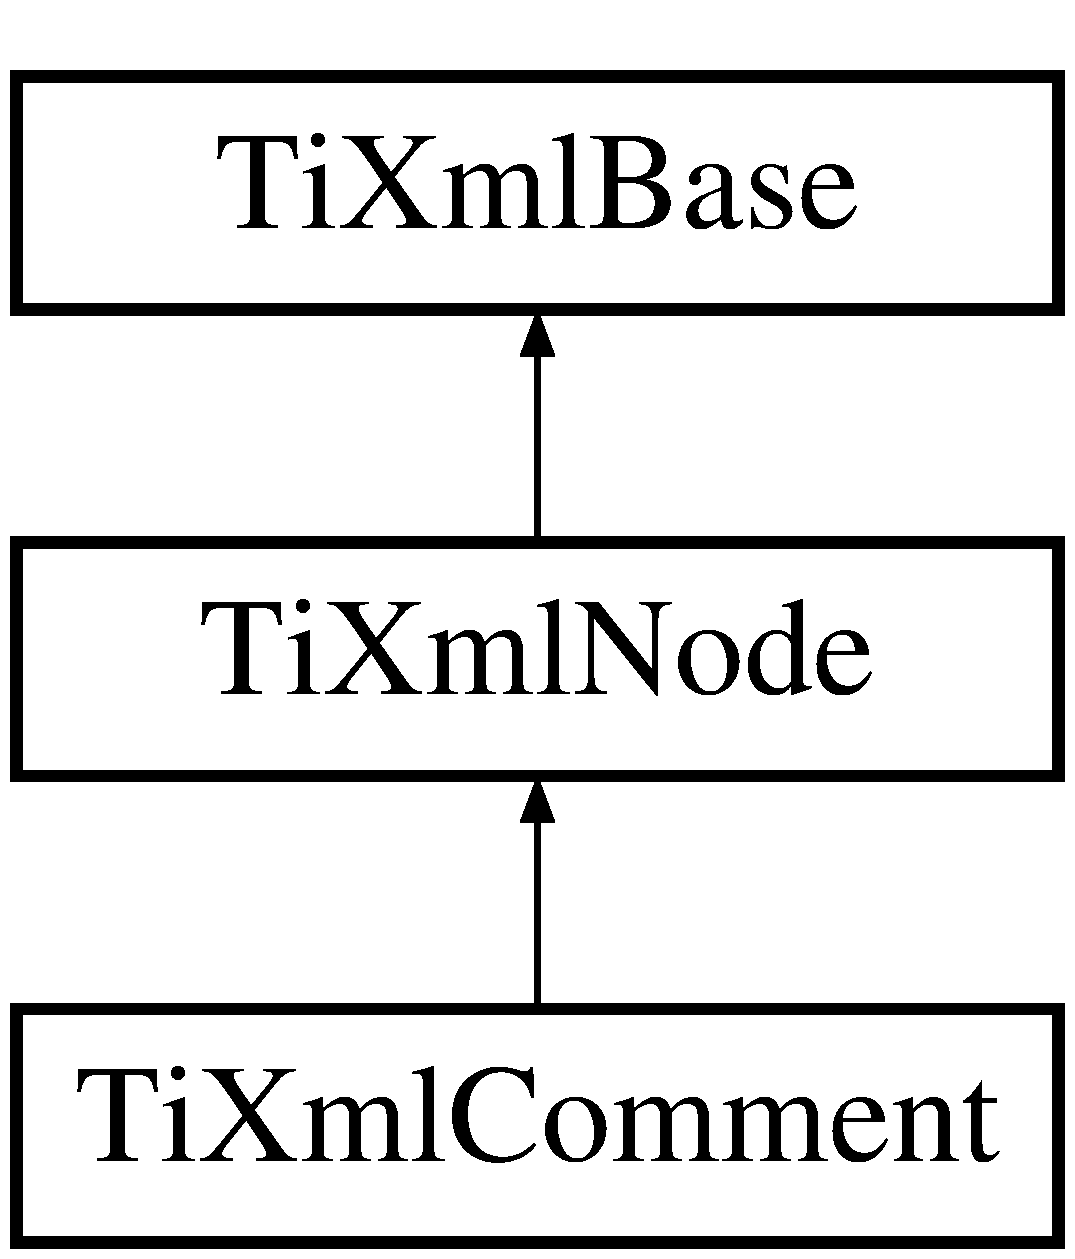
\includegraphics[height=3.000000cm]{class_ti_xml_comment}
\end{center}
\end{figure}
\subsection*{Public Member Functions}
\begin{DoxyCompactItemize}
\item 
\hypertarget{class_ti_xml_comment_aaa3252031d3e8bd3a2bf51a1c61201b7}{
\hyperlink{class_ti_xml_comment_aaa3252031d3e8bd3a2bf51a1c61201b7}{TiXmlComment} ()}
\label{class_ti_xml_comment_aaa3252031d3e8bd3a2bf51a1c61201b7}

\begin{DoxyCompactList}\small\item\em Constructs an empty comment. \end{DoxyCompactList}\item 
\hypertarget{class_ti_xml_comment_a37e7802ef17bc03ebe5ae79bf0713d47}{
\hyperlink{class_ti_xml_comment_a37e7802ef17bc03ebe5ae79bf0713d47}{TiXmlComment} (const char $\ast$\_\-value)}
\label{class_ti_xml_comment_a37e7802ef17bc03ebe5ae79bf0713d47}

\begin{DoxyCompactList}\small\item\em Construct a comment from text. \end{DoxyCompactList}\item 
\hypertarget{class_ti_xml_comment_afaec41ac2760ce946ba1590eb5708e50}{
{\bfseries TiXmlComment} (const \hyperlink{class_ti_xml_comment}{TiXmlComment} \&)}
\label{class_ti_xml_comment_afaec41ac2760ce946ba1590eb5708e50}

\item 
\hypertarget{class_ti_xml_comment_aeceedc15f8b8f9ca0b6136696339b3ac}{
\hyperlink{class_ti_xml_comment}{TiXmlComment} \& {\bfseries operator=} (const \hyperlink{class_ti_xml_comment}{TiXmlComment} \&base)}
\label{class_ti_xml_comment_aeceedc15f8b8f9ca0b6136696339b3ac}

\item 
\hypertarget{class_ti_xml_comment_a4f6590c9c9a2b63a48972655b78eb853}{
virtual \hyperlink{class_ti_xml_node}{TiXmlNode} $\ast$ \hyperlink{class_ti_xml_comment_a4f6590c9c9a2b63a48972655b78eb853}{Clone} () const }
\label{class_ti_xml_comment_a4f6590c9c9a2b63a48972655b78eb853}

\begin{DoxyCompactList}\small\item\em Returns a copy of this Comment. \end{DoxyCompactList}\item 
virtual void \hyperlink{class_ti_xml_comment_a17398061d62c470f57801ce28fa33ad4}{Print} (FILE $\ast$cfile, int depth) const 
\item 
\hypertarget{class_ti_xml_comment_a43bddc18ac057734b41d84653b71d3e0}{
virtual const char $\ast$ {\bfseries Parse} (const char $\ast$p, \hyperlink{class_ti_xml_parsing_data}{TiXmlParsingData} $\ast$data, TiXmlEncoding encoding)}
\label{class_ti_xml_comment_a43bddc18ac057734b41d84653b71d3e0}

\item 
\hypertarget{class_ti_xml_comment_a00fb4215c20a2399ea05ac9b9e7e68a0}{
virtual const \hyperlink{class_ti_xml_comment}{TiXmlComment} $\ast$ \hyperlink{class_ti_xml_comment_a00fb4215c20a2399ea05ac9b9e7e68a0}{ToComment} () const }
\label{class_ti_xml_comment_a00fb4215c20a2399ea05ac9b9e7e68a0}

\begin{DoxyCompactList}\small\item\em Cast to a more defined type. Will return null not of the requested type. \end{DoxyCompactList}\item 
\hypertarget{class_ti_xml_comment_acc7c7e07e13c23f17797d642981511df}{
virtual \hyperlink{class_ti_xml_comment}{TiXmlComment} $\ast$ \hyperlink{class_ti_xml_comment_acc7c7e07e13c23f17797d642981511df}{ToComment} ()}
\label{class_ti_xml_comment_acc7c7e07e13c23f17797d642981511df}

\begin{DoxyCompactList}\small\item\em Cast to a more defined type. Will return null not of the requested type. \end{DoxyCompactList}\item 
virtual bool \hyperlink{class_ti_xml_comment_a4382de0e50da973f11a23ea5852568bd}{Accept} (\hyperlink{class_ti_xml_visitor}{TiXmlVisitor} $\ast$visitor) const 
\end{DoxyCompactItemize}
\subsection*{Protected Member Functions}
\begin{DoxyCompactItemize}
\item 
\hypertarget{class_ti_xml_comment_a3175b2f27628f4fb7a043897930cd934}{
void {\bfseries CopyTo} (\hyperlink{class_ti_xml_comment}{TiXmlComment} $\ast$target) const }
\label{class_ti_xml_comment_a3175b2f27628f4fb7a043897930cd934}

\end{DoxyCompactItemize}


\subsection{Detailed Description}
An XML comment. 

\subsection{Member Function Documentation}
\hypertarget{class_ti_xml_comment_a4382de0e50da973f11a23ea5852568bd}{
\index{TiXmlComment@{TiXmlComment}!Accept@{Accept}}
\index{Accept@{Accept}!TiXmlComment@{TiXmlComment}}
\subsubsection[{Accept}]{\setlength{\rightskip}{0pt plus 5cm}bool TiXmlComment::Accept (
\begin{DoxyParamCaption}
\item[{{\bf TiXmlVisitor} $\ast$}]{visitor}
\end{DoxyParamCaption}
) const\hspace{0.3cm}{\ttfamily  \mbox{[}virtual\mbox{]}}}}
\label{class_ti_xml_comment_a4382de0e50da973f11a23ea5852568bd}
Walk the XML tree visiting this node and all of its children. 

Implements \hyperlink{class_ti_xml_node_acc0f88b7462c6cb73809d410a4f5bb86}{TiXmlNode}.

\hypertarget{class_ti_xml_comment_a17398061d62c470f57801ce28fa33ad4}{
\index{TiXmlComment@{TiXmlComment}!Print@{Print}}
\index{Print@{Print}!TiXmlComment@{TiXmlComment}}
\subsubsection[{Print}]{\setlength{\rightskip}{0pt plus 5cm}void TiXmlComment::Print (
\begin{DoxyParamCaption}
\item[{FILE $\ast$}]{cfile, }
\item[{int}]{depth}
\end{DoxyParamCaption}
) const\hspace{0.3cm}{\ttfamily  \mbox{[}virtual\mbox{]}}}}
\label{class_ti_xml_comment_a17398061d62c470f57801ce28fa33ad4}
All TinyXml classes can print themselves to a filestream or the string class (\hyperlink{class_ti_xml_string}{TiXmlString} in non-\/STL mode, std::string in STL mode.) Either or both cfile and str can be null.

This is a formatted print, and will insert tabs and newlines.

(For an unformatted stream, use the $<$$<$ operator.) 

Implements \hyperlink{class_ti_xml_base_a0de56b3f2ef14c65091a3b916437b512}{TiXmlBase}.



The documentation for this class was generated from the following files:\begin{DoxyCompactItemize}
\item 
/home/cshome/m/mabrams/345/txtEngine/tinyxml.h\item 
/home/cshome/m/mabrams/345/txtEngine/tinyxml.cpp\item 
/home/cshome/m/mabrams/345/txtEngine/tinyxmlparser.cpp\end{DoxyCompactItemize}

\hypertarget{struct_ti_xml_cursor}{
\section{\-Ti\-Xml\-Cursor \-Struct \-Reference}
\label{struct_ti_xml_cursor}\index{\-Ti\-Xml\-Cursor@{\-Ti\-Xml\-Cursor}}
}
\subsection*{\-Public \-Member \-Functions}
\begin{DoxyCompactItemize}
\item 
\hypertarget{struct_ti_xml_cursor_a1e6fa622b59dafb71b6efe595105dcdd}{
void {\bfseries \-Clear} ()}
\label{struct_ti_xml_cursor_a1e6fa622b59dafb71b6efe595105dcdd}

\end{DoxyCompactItemize}
\subsection*{\-Public \-Attributes}
\begin{DoxyCompactItemize}
\item 
\hypertarget{struct_ti_xml_cursor_a5b54dd949820c2db061e2be41f3effb3}{
int {\bfseries row}}
\label{struct_ti_xml_cursor_a5b54dd949820c2db061e2be41f3effb3}

\item 
\hypertarget{struct_ti_xml_cursor_a5694d7ed2c4d20109d350c14c417969d}{
int {\bfseries col}}
\label{struct_ti_xml_cursor_a5694d7ed2c4d20109d350c14c417969d}

\end{DoxyCompactItemize}


\-The documentation for this struct was generated from the following file\-:\begin{DoxyCompactItemize}
\item 
/home/cshome/m/mabrams/345/txt\-Engine/tinyxml.\-h\end{DoxyCompactItemize}

\hypertarget{class_ti_xml_declaration}{
\section{\-Ti\-Xml\-Declaration \-Class \-Reference}
\label{class_ti_xml_declaration}\index{\-Ti\-Xml\-Declaration@{\-Ti\-Xml\-Declaration}}
}


{\ttfamily \#include $<$tinyxml.\-h$>$}

\-Inheritance diagram for \-Ti\-Xml\-Declaration\-:\begin{figure}[H]
\begin{center}
\leavevmode
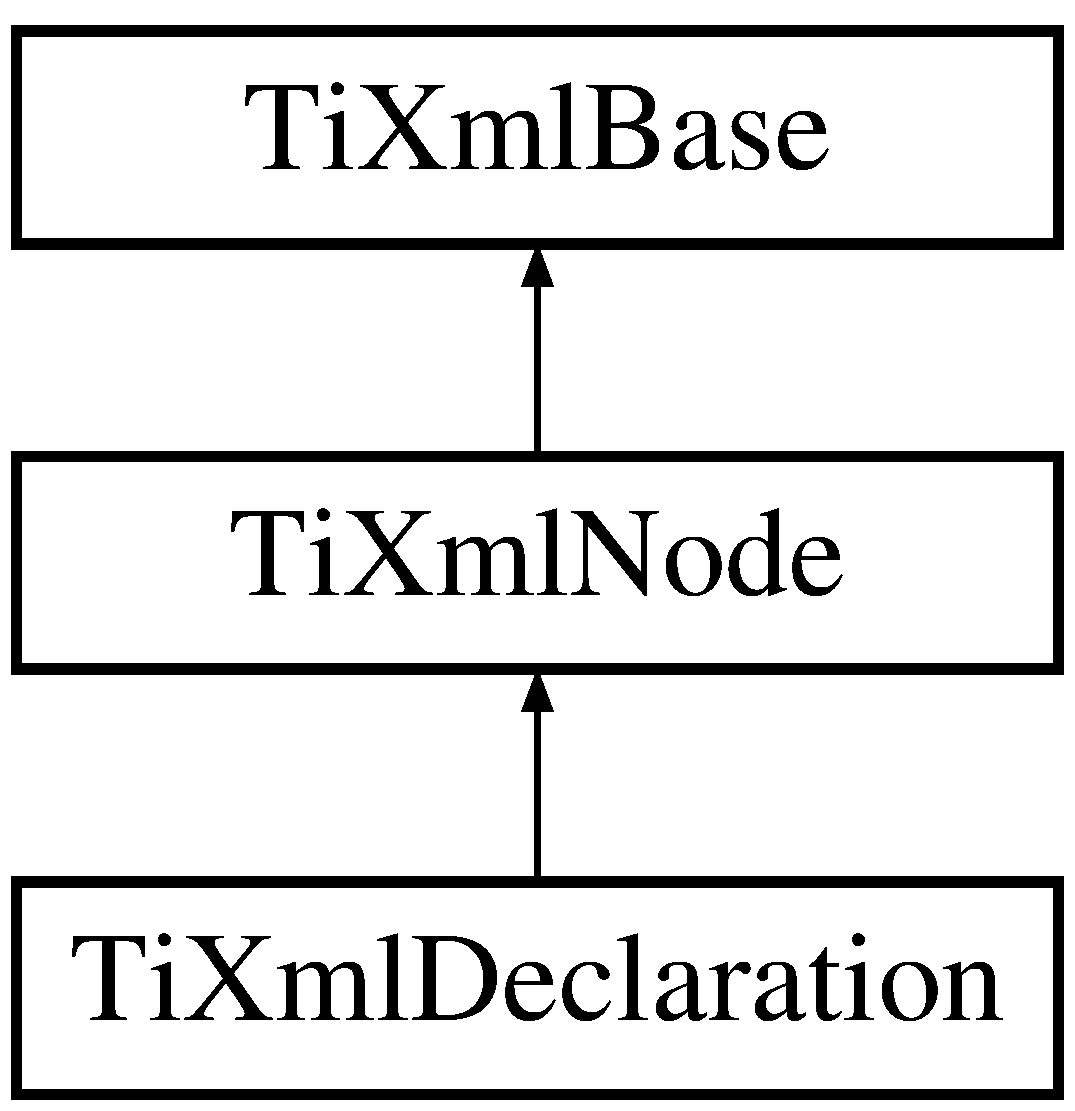
\includegraphics[height=3.000000cm]{class_ti_xml_declaration}
\end{center}
\end{figure}
\subsection*{\-Public \-Member \-Functions}
\begin{DoxyCompactItemize}
\item 
\hypertarget{class_ti_xml_declaration_aa0484d059bea0ea1acb47c9094382d79}{
\hyperlink{class_ti_xml_declaration_aa0484d059bea0ea1acb47c9094382d79}{\-Ti\-Xml\-Declaration} ()}
\label{class_ti_xml_declaration_aa0484d059bea0ea1acb47c9094382d79}

\begin{DoxyCompactList}\small\item\em \-Construct an empty declaration. \end{DoxyCompactList}\item 
\hypertarget{class_ti_xml_declaration_a3b618d1c30c25e4b7a71f31a595ee298}{
\hyperlink{class_ti_xml_declaration_a3b618d1c30c25e4b7a71f31a595ee298}{\-Ti\-Xml\-Declaration} (const char $\ast$\-\_\-version, const char $\ast$\-\_\-encoding, const char $\ast$\-\_\-standalone)}
\label{class_ti_xml_declaration_a3b618d1c30c25e4b7a71f31a595ee298}

\begin{DoxyCompactList}\small\item\em \-Construct. \end{DoxyCompactList}\item 
\hypertarget{class_ti_xml_declaration_a58ac9042c342f7845c8491da0bb091e8}{
{\bfseries \-Ti\-Xml\-Declaration} (const \hyperlink{class_ti_xml_declaration}{\-Ti\-Xml\-Declaration} \&copy)}
\label{class_ti_xml_declaration_a58ac9042c342f7845c8491da0bb091e8}

\item 
\hypertarget{class_ti_xml_declaration_a3bc617efe11014ff2b1a9c5727c37a9a}{
\hyperlink{class_ti_xml_declaration}{\-Ti\-Xml\-Declaration} \& {\bfseries operator=} (const \hyperlink{class_ti_xml_declaration}{\-Ti\-Xml\-Declaration} \&copy)}
\label{class_ti_xml_declaration_a3bc617efe11014ff2b1a9c5727c37a9a}

\item 
\hypertarget{class_ti_xml_declaration_a02ee557b1a4545c3219ed377c103ec76}{
const char $\ast$ \hyperlink{class_ti_xml_declaration_a02ee557b1a4545c3219ed377c103ec76}{\-Version} () const }
\label{class_ti_xml_declaration_a02ee557b1a4545c3219ed377c103ec76}

\begin{DoxyCompactList}\small\item\em \-Version. \-Will return an empty string if none was found. \end{DoxyCompactList}\item 
\hypertarget{class_ti_xml_declaration_a5d974231f9e9a2f0542f15f3a46cdb76}{
const char $\ast$ \hyperlink{class_ti_xml_declaration_a5d974231f9e9a2f0542f15f3a46cdb76}{\-Encoding} () const }
\label{class_ti_xml_declaration_a5d974231f9e9a2f0542f15f3a46cdb76}

\begin{DoxyCompactList}\small\item\em \-Encoding. \-Will return an empty string if none was found. \end{DoxyCompactList}\item 
\hypertarget{class_ti_xml_declaration_a9ff06afc033d7ef730ec7c6825b97ad9}{
const char $\ast$ \hyperlink{class_ti_xml_declaration_a9ff06afc033d7ef730ec7c6825b97ad9}{\-Standalone} () const }
\label{class_ti_xml_declaration_a9ff06afc033d7ef730ec7c6825b97ad9}

\begin{DoxyCompactList}\small\item\em \-Is this a standalone document? \end{DoxyCompactList}\item 
\hypertarget{class_ti_xml_declaration_aff8231266d735943d8a7514a9c9822b9}{
virtual \hyperlink{class_ti_xml_node}{\-Ti\-Xml\-Node} $\ast$ \hyperlink{class_ti_xml_declaration_aff8231266d735943d8a7514a9c9822b9}{\-Clone} () const }
\label{class_ti_xml_declaration_aff8231266d735943d8a7514a9c9822b9}

\begin{DoxyCompactList}\small\item\em \-Creates a copy of this \-Declaration and returns it. \end{DoxyCompactList}\item 
\hypertarget{class_ti_xml_declaration_aa5ab32ec19d4eeecff4a9238c6c90565}{
virtual void {\bfseries \-Print} (\-F\-I\-L\-E $\ast$cfile, int depth, \-T\-I\-X\-M\-L\-\_\-\-S\-T\-R\-I\-N\-G $\ast$str) const }
\label{class_ti_xml_declaration_aa5ab32ec19d4eeecff4a9238c6c90565}

\item 
virtual void \hyperlink{class_ti_xml_declaration_abf6303db4bd05b5be554036817ff1cb4}{\-Print} (\-F\-I\-L\-E $\ast$cfile, int depth) const 
\item 
\hypertarget{class_ti_xml_declaration_a9839ea97ed687a2b7342fd7b0f04361b}{
virtual const char $\ast$ {\bfseries \-Parse} (const char $\ast$p, \hyperlink{class_ti_xml_parsing_data}{\-Ti\-Xml\-Parsing\-Data} $\ast$data, \-Ti\-Xml\-Encoding encoding)}
\label{class_ti_xml_declaration_a9839ea97ed687a2b7342fd7b0f04361b}

\item 
virtual const \hyperlink{class_ti_xml_declaration}{\-Ti\-Xml\-Declaration} $\ast$ \hyperlink{class_ti_xml_declaration_a1e085d3fefd1dbf5ccdbff729931a967}{\-To\-Declaration} () const 
\item 
virtual \hyperlink{class_ti_xml_declaration}{\-Ti\-Xml\-Declaration} $\ast$ \hyperlink{class_ti_xml_declaration_a6bd3d1daddcaeb9543c24bfd090969ce}{\-To\-Declaration} ()
\item 
virtual bool \hyperlink{class_ti_xml_declaration_ab6a6b178161ba9abc2c35058de689864}{\-Accept} (\hyperlink{class_ti_xml_visitor}{\-Ti\-Xml\-Visitor} $\ast$visitor) const 
\end{DoxyCompactItemize}
\subsection*{\-Protected \-Member \-Functions}
\begin{DoxyCompactItemize}
\item 
\hypertarget{class_ti_xml_declaration_a9d08959f935421a593032bd3efb30c38}{
void {\bfseries \-Copy\-To} (\hyperlink{class_ti_xml_declaration}{\-Ti\-Xml\-Declaration} $\ast$target) const }
\label{class_ti_xml_declaration_a9d08959f935421a593032bd3efb30c38}

\end{DoxyCompactItemize}


\subsection{\-Detailed \-Description}
\-In correct \-X\-M\-L the declaration is the first entry in the file. \begin{DoxyVerb}
		<?xml version="1.0" standalone="yes"?>
	\end{DoxyVerb}


\-Tiny\-Xml will happily read or write files without a declaration, however. \-There are 3 possible attributes to the declaration\-: version, encoding, and standalone.

\-Note\-: \-In this version of the code, the attributes are handled as special cases, not generic attributes, simply because there can only be at most 3 and they are always the same. 

\subsection{\-Member \-Function \-Documentation}
\hypertarget{class_ti_xml_declaration_ab6a6b178161ba9abc2c35058de689864}{
\index{\-Ti\-Xml\-Declaration@{\-Ti\-Xml\-Declaration}!\-Accept@{\-Accept}}
\index{\-Accept@{\-Accept}!TiXmlDeclaration@{\-Ti\-Xml\-Declaration}}
\subsubsection[{\-Accept}]{\setlength{\rightskip}{0pt plus 5cm}bool \-Ti\-Xml\-Declaration\-::\-Accept (
\begin{DoxyParamCaption}
\item[{{\bf \-Ti\-Xml\-Visitor} $\ast$}]{visitor}
\end{DoxyParamCaption}
) const\hspace{0.3cm}{\ttfamily  \mbox{[}virtual\mbox{]}}}}
\label{class_ti_xml_declaration_ab6a6b178161ba9abc2c35058de689864}
\-Walk the \-X\-M\-L tree visiting this node and all of its children. 

\-Implements \hyperlink{class_ti_xml_node_acc0f88b7462c6cb73809d410a4f5bb86}{\-Ti\-Xml\-Node}.

\hypertarget{class_ti_xml_declaration_abf6303db4bd05b5be554036817ff1cb4}{
\index{\-Ti\-Xml\-Declaration@{\-Ti\-Xml\-Declaration}!\-Print@{\-Print}}
\index{\-Print@{\-Print}!TiXmlDeclaration@{\-Ti\-Xml\-Declaration}}
\subsubsection[{\-Print}]{\setlength{\rightskip}{0pt plus 5cm}virtual void \-Ti\-Xml\-Declaration\-::\-Print (
\begin{DoxyParamCaption}
\item[{\-F\-I\-L\-E $\ast$}]{cfile, }
\item[{int}]{depth}
\end{DoxyParamCaption}
) const\hspace{0.3cm}{\ttfamily  \mbox{[}inline, virtual\mbox{]}}}}
\label{class_ti_xml_declaration_abf6303db4bd05b5be554036817ff1cb4}
\-All \-Tiny\-Xml classes can print themselves to a filestream or the string class (\hyperlink{class_ti_xml_string}{\-Ti\-Xml\-String} in non-\/\-S\-T\-L mode, std\-::string in \-S\-T\-L mode.) \-Either or both cfile and str can be null.

\-This is a formatted print, and will insert tabs and newlines.

(\-For an unformatted stream, use the $<$$<$ operator.) 

\-Implements \hyperlink{class_ti_xml_base_a0de56b3f2ef14c65091a3b916437b512}{\-Ti\-Xml\-Base}.

\hypertarget{class_ti_xml_declaration_a1e085d3fefd1dbf5ccdbff729931a967}{
\index{\-Ti\-Xml\-Declaration@{\-Ti\-Xml\-Declaration}!\-To\-Declaration@{\-To\-Declaration}}
\index{\-To\-Declaration@{\-To\-Declaration}!TiXmlDeclaration@{\-Ti\-Xml\-Declaration}}
\subsubsection[{\-To\-Declaration}]{\setlength{\rightskip}{0pt plus 5cm}virtual const {\bf \-Ti\-Xml\-Declaration}$\ast$ \-Ti\-Xml\-Declaration\-::\-To\-Declaration (
\begin{DoxyParamCaption}
{}
\end{DoxyParamCaption}
) const\hspace{0.3cm}{\ttfamily  \mbox{[}inline, virtual\mbox{]}}}}
\label{class_ti_xml_declaration_a1e085d3fefd1dbf5ccdbff729931a967}
$<$ \-Cast to a more defined type. \-Will return null not of the requested type. 

\-Reimplemented from \hyperlink{class_ti_xml_node_a9f43e6984fc7d4afd6eb32714c6b7b72}{\-Ti\-Xml\-Node}.

\hypertarget{class_ti_xml_declaration_a6bd3d1daddcaeb9543c24bfd090969ce}{
\index{\-Ti\-Xml\-Declaration@{\-Ti\-Xml\-Declaration}!\-To\-Declaration@{\-To\-Declaration}}
\index{\-To\-Declaration@{\-To\-Declaration}!TiXmlDeclaration@{\-Ti\-Xml\-Declaration}}
\subsubsection[{\-To\-Declaration}]{\setlength{\rightskip}{0pt plus 5cm}virtual {\bf \-Ti\-Xml\-Declaration}$\ast$ \-Ti\-Xml\-Declaration\-::\-To\-Declaration (
\begin{DoxyParamCaption}
{}
\end{DoxyParamCaption}
)\hspace{0.3cm}{\ttfamily  \mbox{[}inline, virtual\mbox{]}}}}
\label{class_ti_xml_declaration_a6bd3d1daddcaeb9543c24bfd090969ce}
$<$ \-Cast to a more defined type. \-Will return null not of the requested type. 

\-Reimplemented from \hyperlink{class_ti_xml_node_a4027136ca820ff4a636b607231b6a6df}{\-Ti\-Xml\-Node}.



\-The documentation for this class was generated from the following files\-:\begin{DoxyCompactItemize}
\item 
/home/cshome/m/mabrams/345/txt\-Engine/tinyxml.\-h\item 
/home/cshome/m/mabrams/345/txt\-Engine/tinyxml.\-cpp\item 
/home/cshome/m/mabrams/345/txt\-Engine/tinyxmlparser.\-cpp\end{DoxyCompactItemize}

\hypertarget{class_ti_xml_document}{
\section{\-Ti\-Xml\-Document \-Class \-Reference}
\label{class_ti_xml_document}\index{\-Ti\-Xml\-Document@{\-Ti\-Xml\-Document}}
}


{\ttfamily \#include $<$tinyxml.\-h$>$}



\-Inheritance diagram for \-Ti\-Xml\-Document\-:


\-Collaboration diagram for \-Ti\-Xml\-Document\-:
\subsection*{\-Public \-Member \-Functions}
\begin{DoxyCompactItemize}
\item 
\hypertarget{class_ti_xml_document_a9f5e84335708fde98400230f9f12659c}{
\hyperlink{class_ti_xml_document_a9f5e84335708fde98400230f9f12659c}{\-Ti\-Xml\-Document} ()}
\label{class_ti_xml_document_a9f5e84335708fde98400230f9f12659c}

\begin{DoxyCompactList}\small\item\em \-Create an empty document, that has no name. \end{DoxyCompactList}\item 
\hypertarget{class_ti_xml_document_ae4508b452d0c3061db085f3db27b8396}{
\hyperlink{class_ti_xml_document_ae4508b452d0c3061db085f3db27b8396}{\-Ti\-Xml\-Document} (const char $\ast$document\-Name)}
\label{class_ti_xml_document_ae4508b452d0c3061db085f3db27b8396}

\begin{DoxyCompactList}\small\item\em \-Create a document with a name. \-The name of the document is also the filename of the xml. \end{DoxyCompactList}\item 
\hypertarget{class_ti_xml_document_a323a7486e7da6099cdc19a5ff7e74b07}{
{\bfseries \-Ti\-Xml\-Document} (const \hyperlink{class_ti_xml_document}{\-Ti\-Xml\-Document} \&copy)}
\label{class_ti_xml_document_a323a7486e7da6099cdc19a5ff7e74b07}

\item 
\hypertarget{class_ti_xml_document_aa56fd4dbe8917d2033d865909e2d737e}{
\hyperlink{class_ti_xml_document}{\-Ti\-Xml\-Document} \& {\bfseries operator=} (const \hyperlink{class_ti_xml_document}{\-Ti\-Xml\-Document} \&copy)}
\label{class_ti_xml_document_aa56fd4dbe8917d2033d865909e2d737e}

\item 
bool \hyperlink{class_ti_xml_document_a4c852a889c02cf251117fd1d9fe1845f}{\-Load\-File} (\-Ti\-Xml\-Encoding encoding=\-T\-I\-X\-M\-L\-\_\-\-D\-E\-F\-A\-U\-L\-T\-\_\-\-E\-N\-C\-O\-D\-I\-N\-G)
\item 
\hypertarget{class_ti_xml_document_a21c0aeb0d0a720169ad4ac89523ebe93}{
bool \hyperlink{class_ti_xml_document_a21c0aeb0d0a720169ad4ac89523ebe93}{\-Save\-File} () const }
\label{class_ti_xml_document_a21c0aeb0d0a720169ad4ac89523ebe93}

\begin{DoxyCompactList}\small\item\em \-Save a file using the current document value. \-Returns true if successful. \end{DoxyCompactList}\item 
\hypertarget{class_ti_xml_document_a879cdf5e981b8b2d2ef82f2546dd28fb}{
bool \hyperlink{class_ti_xml_document_a879cdf5e981b8b2d2ef82f2546dd28fb}{\-Load\-File} (const char $\ast$filename, \-Ti\-Xml\-Encoding encoding=\-T\-I\-X\-M\-L\-\_\-\-D\-E\-F\-A\-U\-L\-T\-\_\-\-E\-N\-C\-O\-D\-I\-N\-G)}
\label{class_ti_xml_document_a879cdf5e981b8b2d2ef82f2546dd28fb}

\begin{DoxyCompactList}\small\item\em \-Load a file using the given filename. \-Returns true if successful. \end{DoxyCompactList}\item 
\hypertarget{class_ti_xml_document_ae869f5ebf7fc54c4a1d737fb4689fd44}{
bool \hyperlink{class_ti_xml_document_ae869f5ebf7fc54c4a1d737fb4689fd44}{\-Save\-File} (const char $\ast$filename) const }
\label{class_ti_xml_document_ae869f5ebf7fc54c4a1d737fb4689fd44}

\begin{DoxyCompactList}\small\item\em \-Save a file using the given filename. \-Returns true if successful. \end{DoxyCompactList}\item 
bool \hyperlink{class_ti_xml_document_a41f6fe7200864d1dca663d230caf8db6}{\-Load\-File} (\-F\-I\-L\-E $\ast$, \-Ti\-Xml\-Encoding encoding=\-T\-I\-X\-M\-L\-\_\-\-D\-E\-F\-A\-U\-L\-T\-\_\-\-E\-N\-C\-O\-D\-I\-N\-G)
\item 
\hypertarget{class_ti_xml_document_acf1672b4538c6d1d441f9f108aea2bf4}{
bool \hyperlink{class_ti_xml_document_acf1672b4538c6d1d441f9f108aea2bf4}{\-Save\-File} (\-F\-I\-L\-E $\ast$) const }
\label{class_ti_xml_document_acf1672b4538c6d1d441f9f108aea2bf4}

\begin{DoxyCompactList}\small\item\em \-Save a file using the given \-F\-I\-L\-E$\ast$. \-Returns true if successful. \end{DoxyCompactList}\item 
virtual const char $\ast$ \hyperlink{class_ti_xml_document_a789ad2f06f93d52bdb5570b2f3670289}{\-Parse} (const char $\ast$p, \hyperlink{class_ti_xml_parsing_data}{\-Ti\-Xml\-Parsing\-Data} $\ast$data=0, \-Ti\-Xml\-Encoding encoding=\-T\-I\-X\-M\-L\-\_\-\-D\-E\-F\-A\-U\-L\-T\-\_\-\-E\-N\-C\-O\-D\-I\-N\-G)
\item 
const \hyperlink{class_ti_xml_element}{\-Ti\-Xml\-Element} $\ast$ \hyperlink{class_ti_xml_document_ad09d17927f908f40efb406af2fb873be}{\-Root\-Element} () const 
\item 
\hypertarget{class_ti_xml_document_a0b43e762a23f938b06651bc90b8a1013}{
\hyperlink{class_ti_xml_element}{\-Ti\-Xml\-Element} $\ast$ {\bfseries \-Root\-Element} ()}
\label{class_ti_xml_document_a0b43e762a23f938b06651bc90b8a1013}

\item 
bool \hyperlink{class_ti_xml_document_a6dfc01a6e5d58e56acd537dfd3bdeb29}{\-Error} () const 
\item 
\hypertarget{class_ti_xml_document_a9d0f689f6e09ea494ea547be8d79c25e}{
const char $\ast$ \hyperlink{class_ti_xml_document_a9d0f689f6e09ea494ea547be8d79c25e}{\-Error\-Desc} () const }
\label{class_ti_xml_document_a9d0f689f6e09ea494ea547be8d79c25e}

\begin{DoxyCompactList}\small\item\em \-Contains a textual (english) description of the error if one occurs. \end{DoxyCompactList}\item 
int \hyperlink{class_ti_xml_document_af96fc2f3f9ec6422782bfe916c9e778f}{\-Error\-Id} () const 
\item 
int \hyperlink{class_ti_xml_document_af30efc75e804aa2e92fb8be3a8cb676e}{\-Error\-Row} () const 
\item 
int \hyperlink{class_ti_xml_document_aa90bc630ee5203c6109ca5fad3323649}{\-Error\-Col} () const 
\item 
void \hyperlink{class_ti_xml_document_a51dac56316f89b35bdb7d0d433ba988e}{\-Set\-Tab\-Size} (int \-\_\-tabsize)
\item 
\hypertarget{class_ti_xml_document_a612360241b85bad0826b2a9ae9cda561}{
int {\bfseries \-Tab\-Size} () const }
\label{class_ti_xml_document_a612360241b85bad0826b2a9ae9cda561}

\item 
void \hyperlink{class_ti_xml_document_ac66b8c28db86363315712a3574e87c35}{\-Clear\-Error} ()
\item 
void \hyperlink{class_ti_xml_document_af08389ec70ee9b2de7f800e206a18510}{\-Print} () const 
\item 
\hypertarget{class_ti_xml_document_a7b1aea204fee266b70b9c105c8bf2ada}{
virtual void \hyperlink{class_ti_xml_document_a7b1aea204fee266b70b9c105c8bf2ada}{\-Print} (\-F\-I\-L\-E $\ast$cfile, int depth=0) const }
\label{class_ti_xml_document_a7b1aea204fee266b70b9c105c8bf2ada}

\begin{DoxyCompactList}\small\item\em \-Print this \-Document to a \-F\-I\-L\-E stream. \end{DoxyCompactList}\item 
\hypertarget{class_ti_xml_document_a735c23e318597b920c94eae77fa206de}{
void {\bfseries \-Set\-Error} (int err, const char $\ast$error\-Location, \hyperlink{class_ti_xml_parsing_data}{\-Ti\-Xml\-Parsing\-Data} $\ast$prev\-Data, \-Ti\-Xml\-Encoding encoding)}
\label{class_ti_xml_document_a735c23e318597b920c94eae77fa206de}

\item 
virtual const \hyperlink{class_ti_xml_document}{\-Ti\-Xml\-Document} $\ast$ \hyperlink{class_ti_xml_document_a1dc977bde3e4fe85a8eb9d88a35ef5a4}{\-To\-Document} () const 
\item 
virtual \hyperlink{class_ti_xml_document}{\-Ti\-Xml\-Document} $\ast$ \hyperlink{class_ti_xml_document_a1025d942a1f328fd742d545e37efdd42}{\-To\-Document} ()
\item 
virtual bool \hyperlink{class_ti_xml_document_a3daab2f472418ef66315750202f762ae}{\-Accept} (\hyperlink{class_ti_xml_visitor}{\-Ti\-Xml\-Visitor} $\ast$content) const 
\end{DoxyCompactItemize}
\subsection*{\-Protected \-Member \-Functions}
\begin{DoxyCompactItemize}
\item 
virtual \hyperlink{class_ti_xml_node}{\-Ti\-Xml\-Node} $\ast$ \hyperlink{class_ti_xml_document_ac9e8f09b23454d953b32d1b65cd1409e}{\-Clone} () const 
\end{DoxyCompactItemize}


\subsection{\-Detailed \-Description}
\-Always the top level node. \-A document binds together all the \-X\-M\-L pieces. \-It can be saved, loaded, and printed to the screen. \-The 'value' of a document node is the xml file name. 

\subsection{\-Member \-Function \-Documentation}
\hypertarget{class_ti_xml_document_a3daab2f472418ef66315750202f762ae}{
\index{\-Ti\-Xml\-Document@{\-Ti\-Xml\-Document}!\-Accept@{\-Accept}}
\index{\-Accept@{\-Accept}!TiXmlDocument@{\-Ti\-Xml\-Document}}
\subsubsection[{\-Accept}]{\setlength{\rightskip}{0pt plus 5cm}bool \-Ti\-Xml\-Document\-::\-Accept (
\begin{DoxyParamCaption}
\item[{{\bf \-Ti\-Xml\-Visitor} $\ast$}]{content}
\end{DoxyParamCaption}
) const\hspace{0.3cm}{\ttfamily  \mbox{[}virtual\mbox{]}}}}
\label{class_ti_xml_document_a3daab2f472418ef66315750202f762ae}
\-Walk the \-X\-M\-L tree visiting this node and all of its children. 

\-Implements \hyperlink{class_ti_xml_node_acc0f88b7462c6cb73809d410a4f5bb86}{\-Ti\-Xml\-Node}.



\-Here is the call graph for this function\-:


\hypertarget{class_ti_xml_document_ac66b8c28db86363315712a3574e87c35}{
\index{\-Ti\-Xml\-Document@{\-Ti\-Xml\-Document}!\-Clear\-Error@{\-Clear\-Error}}
\index{\-Clear\-Error@{\-Clear\-Error}!TiXmlDocument@{\-Ti\-Xml\-Document}}
\subsubsection[{\-Clear\-Error}]{\setlength{\rightskip}{0pt plus 5cm}void \-Ti\-Xml\-Document\-::\-Clear\-Error (
\begin{DoxyParamCaption}
{}
\end{DoxyParamCaption}
)\hspace{0.3cm}{\ttfamily  \mbox{[}inline\mbox{]}}}}
\label{class_ti_xml_document_ac66b8c28db86363315712a3574e87c35}
\-If you have handled the error, it can be reset with this call. \-The error state is automatically cleared if you \-Parse a new \-X\-M\-L block. 

\-Here is the caller graph for this function\-:


\hypertarget{class_ti_xml_document_ac9e8f09b23454d953b32d1b65cd1409e}{
\index{\-Ti\-Xml\-Document@{\-Ti\-Xml\-Document}!\-Clone@{\-Clone}}
\index{\-Clone@{\-Clone}!TiXmlDocument@{\-Ti\-Xml\-Document}}
\subsubsection[{\-Clone}]{\setlength{\rightskip}{0pt plus 5cm}{\bf \-Ti\-Xml\-Node} $\ast$ \-Ti\-Xml\-Document\-::\-Clone (
\begin{DoxyParamCaption}
{}
\end{DoxyParamCaption}
) const\hspace{0.3cm}{\ttfamily  \mbox{[}protected, virtual\mbox{]}}}}
\label{class_ti_xml_document_ac9e8f09b23454d953b32d1b65cd1409e}
\-Create an exact duplicate of this node and return it. \-The memory must be deleted by the caller. 

\-Implements \hyperlink{class_ti_xml_node_a4508cc3a2d7a98e96a54cc09c37a78a4}{\-Ti\-Xml\-Node}.



\-Here is the call graph for this function\-:


\hypertarget{class_ti_xml_document_a6dfc01a6e5d58e56acd537dfd3bdeb29}{
\index{\-Ti\-Xml\-Document@{\-Ti\-Xml\-Document}!\-Error@{\-Error}}
\index{\-Error@{\-Error}!TiXmlDocument@{\-Ti\-Xml\-Document}}
\subsubsection[{\-Error}]{\setlength{\rightskip}{0pt plus 5cm}bool \-Ti\-Xml\-Document\-::\-Error (
\begin{DoxyParamCaption}
{}
\end{DoxyParamCaption}
) const\hspace{0.3cm}{\ttfamily  \mbox{[}inline\mbox{]}}}}
\label{class_ti_xml_document_a6dfc01a6e5d58e56acd537dfd3bdeb29}
\-If an error occurs, \-Error will be set to true. \-Also,
\begin{DoxyItemize}
\item \-The \hyperlink{class_ti_xml_document_af96fc2f3f9ec6422782bfe916c9e778f}{\-Error\-Id()} will contain the integer identifier of the error (not generally useful)
\item \-The \hyperlink{class_ti_xml_document_a9d0f689f6e09ea494ea547be8d79c25e}{\-Error\-Desc()} method will return the name of the error. (very useful)
\item \-The \hyperlink{class_ti_xml_document_af30efc75e804aa2e92fb8be3a8cb676e}{\-Error\-Row()} and \hyperlink{class_ti_xml_document_aa90bc630ee5203c6109ca5fad3323649}{\-Error\-Col()} will return the location of the error (if known) 
\end{DoxyItemize}

\-Here is the caller graph for this function\-:


\hypertarget{class_ti_xml_document_aa90bc630ee5203c6109ca5fad3323649}{
\index{\-Ti\-Xml\-Document@{\-Ti\-Xml\-Document}!\-Error\-Col@{\-Error\-Col}}
\index{\-Error\-Col@{\-Error\-Col}!TiXmlDocument@{\-Ti\-Xml\-Document}}
\subsubsection[{\-Error\-Col}]{\setlength{\rightskip}{0pt plus 5cm}int \-Ti\-Xml\-Document\-::\-Error\-Col (
\begin{DoxyParamCaption}
{}
\end{DoxyParamCaption}
) const\hspace{0.3cm}{\ttfamily  \mbox{[}inline\mbox{]}}}}
\label{class_ti_xml_document_aa90bc630ee5203c6109ca5fad3323649}
$<$ \-The column where the error occured. \-See \hyperlink{class_ti_xml_document_af30efc75e804aa2e92fb8be3a8cb676e}{\-Error\-Row()} \hypertarget{class_ti_xml_document_af96fc2f3f9ec6422782bfe916c9e778f}{
\index{\-Ti\-Xml\-Document@{\-Ti\-Xml\-Document}!\-Error\-Id@{\-Error\-Id}}
\index{\-Error\-Id@{\-Error\-Id}!TiXmlDocument@{\-Ti\-Xml\-Document}}
\subsubsection[{\-Error\-Id}]{\setlength{\rightskip}{0pt plus 5cm}int \-Ti\-Xml\-Document\-::\-Error\-Id (
\begin{DoxyParamCaption}
{}
\end{DoxyParamCaption}
) const\hspace{0.3cm}{\ttfamily  \mbox{[}inline\mbox{]}}}}
\label{class_ti_xml_document_af96fc2f3f9ec6422782bfe916c9e778f}
\-Generally, you probably want the error string ( \hyperlink{class_ti_xml_document_a9d0f689f6e09ea494ea547be8d79c25e}{\-Error\-Desc()} ). \-But if you prefer the \-Error\-Id, this function will fetch it. \hypertarget{class_ti_xml_document_af30efc75e804aa2e92fb8be3a8cb676e}{
\index{\-Ti\-Xml\-Document@{\-Ti\-Xml\-Document}!\-Error\-Row@{\-Error\-Row}}
\index{\-Error\-Row@{\-Error\-Row}!TiXmlDocument@{\-Ti\-Xml\-Document}}
\subsubsection[{\-Error\-Row}]{\setlength{\rightskip}{0pt plus 5cm}int \-Ti\-Xml\-Document\-::\-Error\-Row (
\begin{DoxyParamCaption}
{}
\end{DoxyParamCaption}
) const\hspace{0.3cm}{\ttfamily  \mbox{[}inline\mbox{]}}}}
\label{class_ti_xml_document_af30efc75e804aa2e92fb8be3a8cb676e}
\-Returns the location (if known) of the error. \-The first column is column 1, and the first row is row 1. \-A value of 0 means the row and column wasn't applicable (memory errors, for example, have no row/column) or the parser lost the error. (\-An error in the error reporting, in that case.)

\begin{DoxySeeAlso}{\-See also}
\hyperlink{class_ti_xml_document_a51dac56316f89b35bdb7d0d433ba988e}{\-Set\-Tab\-Size}, \hyperlink{class_ti_xml_base_a024bceb070188df92c2a8d8852dd0853}{\-Row}, \hyperlink{class_ti_xml_base_ab54bfb9b70fe6dd276e7b279cab7f003}{\-Column} 
\end{DoxySeeAlso}
\hypertarget{class_ti_xml_document_a4c852a889c02cf251117fd1d9fe1845f}{
\index{\-Ti\-Xml\-Document@{\-Ti\-Xml\-Document}!\-Load\-File@{\-Load\-File}}
\index{\-Load\-File@{\-Load\-File}!TiXmlDocument@{\-Ti\-Xml\-Document}}
\subsubsection[{\-Load\-File}]{\setlength{\rightskip}{0pt plus 5cm}bool \-Ti\-Xml\-Document\-::\-Load\-File (
\begin{DoxyParamCaption}
\item[{\-Ti\-Xml\-Encoding}]{encoding = {\ttfamily \-T\-I\-X\-M\-L\-\_\-\-D\-E\-F\-A\-U\-L\-T\-\_\-\-E\-N\-C\-O\-D\-I\-N\-G}}
\end{DoxyParamCaption}
)}}
\label{class_ti_xml_document_a4c852a889c02cf251117fd1d9fe1845f}
\-Load a file using the current document value. \-Returns true if successful. \-Will delete any existing document data before loading. 

\-Here is the call graph for this function\-:




\-Here is the caller graph for this function\-:


\hypertarget{class_ti_xml_document_a41f6fe7200864d1dca663d230caf8db6}{
\index{\-Ti\-Xml\-Document@{\-Ti\-Xml\-Document}!\-Load\-File@{\-Load\-File}}
\index{\-Load\-File@{\-Load\-File}!TiXmlDocument@{\-Ti\-Xml\-Document}}
\subsubsection[{\-Load\-File}]{\setlength{\rightskip}{0pt plus 5cm}bool \-Ti\-Xml\-Document\-::\-Load\-File (
\begin{DoxyParamCaption}
\item[{\-F\-I\-L\-E $\ast$}]{file, }
\item[{\-Ti\-Xml\-Encoding}]{encoding = {\ttfamily \-T\-I\-X\-M\-L\-\_\-\-D\-E\-F\-A\-U\-L\-T\-\_\-\-E\-N\-C\-O\-D\-I\-N\-G}}
\end{DoxyParamCaption}
)}}
\label{class_ti_xml_document_a41f6fe7200864d1dca663d230caf8db6}
\-Load a file using the given \-F\-I\-L\-E$\ast$. \-Returns true if successful. \-Note that this method doesn't stream -\/ the entire object pointed at by the \-F\-I\-L\-E$\ast$ will be interpreted as an \-X\-M\-L file. \-Tiny\-X\-M\-L doesn't stream in \-X\-M\-L from the current file location. \-Streaming may be added in the future. 

\-Here is the call graph for this function\-:


\hypertarget{class_ti_xml_document_a789ad2f06f93d52bdb5570b2f3670289}{
\index{\-Ti\-Xml\-Document@{\-Ti\-Xml\-Document}!\-Parse@{\-Parse}}
\index{\-Parse@{\-Parse}!TiXmlDocument@{\-Ti\-Xml\-Document}}
\subsubsection[{\-Parse}]{\setlength{\rightskip}{0pt plus 5cm}const char $\ast$ \-Ti\-Xml\-Document\-::\-Parse (
\begin{DoxyParamCaption}
\item[{const char $\ast$}]{p, }
\item[{{\bf \-Ti\-Xml\-Parsing\-Data} $\ast$}]{data = {\ttfamily 0}, }
\item[{\-Ti\-Xml\-Encoding}]{encoding = {\ttfamily \-T\-I\-X\-M\-L\-\_\-\-D\-E\-F\-A\-U\-L\-T\-\_\-\-E\-N\-C\-O\-D\-I\-N\-G}}
\end{DoxyParamCaption}
)\hspace{0.3cm}{\ttfamily  \mbox{[}virtual\mbox{]}}}}
\label{class_ti_xml_document_a789ad2f06f93d52bdb5570b2f3670289}
\-Parse the given null terminated block of xml data. \-Passing in an encoding to this method (either \-T\-I\-X\-M\-L\-\_\-\-E\-N\-C\-O\-D\-I\-N\-G\-\_\-\-L\-E\-G\-A\-C\-Y or \-T\-I\-X\-M\-L\-\_\-\-E\-N\-C\-O\-D\-I\-N\-G\-\_\-\-U\-T\-F8 will force \-Tiny\-Xml to use that encoding, regardless of what \-Tiny\-Xml might otherwise try to detect. 

\-Implements \hyperlink{class_ti_xml_base}{\-Ti\-Xml\-Base}.



\-Here is the call graph for this function\-:




\-Here is the caller graph for this function\-:


\hypertarget{class_ti_xml_document_af08389ec70ee9b2de7f800e206a18510}{
\index{\-Ti\-Xml\-Document@{\-Ti\-Xml\-Document}!\-Print@{\-Print}}
\index{\-Print@{\-Print}!TiXmlDocument@{\-Ti\-Xml\-Document}}
\subsubsection[{\-Print}]{\setlength{\rightskip}{0pt plus 5cm}void \-Ti\-Xml\-Document\-::\-Print (
\begin{DoxyParamCaption}
{}
\end{DoxyParamCaption}
) const\hspace{0.3cm}{\ttfamily  \mbox{[}inline\mbox{]}}}}
\label{class_ti_xml_document_af08389ec70ee9b2de7f800e206a18510}
\-Write the document to standard out using formatted printing (\char`\"{}pretty print\char`\"{}). 

\-Here is the caller graph for this function\-:


\hypertarget{class_ti_xml_document_ad09d17927f908f40efb406af2fb873be}{
\index{\-Ti\-Xml\-Document@{\-Ti\-Xml\-Document}!\-Root\-Element@{\-Root\-Element}}
\index{\-Root\-Element@{\-Root\-Element}!TiXmlDocument@{\-Ti\-Xml\-Document}}
\subsubsection[{\-Root\-Element}]{\setlength{\rightskip}{0pt plus 5cm}const {\bf \-Ti\-Xml\-Element}$\ast$ \-Ti\-Xml\-Document\-::\-Root\-Element (
\begin{DoxyParamCaption}
{}
\end{DoxyParamCaption}
) const\hspace{0.3cm}{\ttfamily  \mbox{[}inline\mbox{]}}}}
\label{class_ti_xml_document_ad09d17927f908f40efb406af2fb873be}
\-Get the root element -\/-\/ the only top level element -\/-\/ of the document. \-In well formed \-X\-M\-L, there should only be one. \-Tiny\-Xml is tolerant of multiple elements at the document level. 

\-Here is the call graph for this function\-:


\hypertarget{class_ti_xml_document_a51dac56316f89b35bdb7d0d433ba988e}{
\index{\-Ti\-Xml\-Document@{\-Ti\-Xml\-Document}!\-Set\-Tab\-Size@{\-Set\-Tab\-Size}}
\index{\-Set\-Tab\-Size@{\-Set\-Tab\-Size}!TiXmlDocument@{\-Ti\-Xml\-Document}}
\subsubsection[{\-Set\-Tab\-Size}]{\setlength{\rightskip}{0pt plus 5cm}void \-Ti\-Xml\-Document\-::\-Set\-Tab\-Size (
\begin{DoxyParamCaption}
\item[{int}]{\-\_\-tabsize}
\end{DoxyParamCaption}
)\hspace{0.3cm}{\ttfamily  \mbox{[}inline\mbox{]}}}}
\label{class_ti_xml_document_a51dac56316f89b35bdb7d0d433ba988e}
\hyperlink{class_ti_xml_document_a51dac56316f89b35bdb7d0d433ba988e}{\-Set\-Tab\-Size()} allows the error reporting functions (\hyperlink{class_ti_xml_document_af30efc75e804aa2e92fb8be3a8cb676e}{\-Error\-Row()} and \hyperlink{class_ti_xml_document_aa90bc630ee5203c6109ca5fad3323649}{\-Error\-Col()}) to report the correct values for row and column. \-It does not change the output or input in any way.

\-By calling this method, with a tab size greater than 0, the row and column of each node and attribute is stored when the file is loaded. \-Very useful for tracking the \-D\-O\-M back in to the source file.

\-The tab size is required for calculating the location of nodes. \-If not set, the default of 4 is used. \-The tabsize is set per document. \-Setting the tabsize to 0 disables row/column tracking.

\-Note that row and column tracking is not supported when using operator$>$$>$.

\-The tab size needs to be enabled before the parse or load. \-Correct usage\-: \begin{DoxyVerb}
        	TiXmlDocument doc;
        	doc.SetTabSize( 8 );
        	doc.Load( "myfile.xml" );
        	\end{DoxyVerb}


\begin{DoxySeeAlso}{\-See also}
\hyperlink{class_ti_xml_base_a024bceb070188df92c2a8d8852dd0853}{\-Row}, \hyperlink{class_ti_xml_base_ab54bfb9b70fe6dd276e7b279cab7f003}{\-Column} 
\end{DoxySeeAlso}
\hypertarget{class_ti_xml_document_a1dc977bde3e4fe85a8eb9d88a35ef5a4}{
\index{\-Ti\-Xml\-Document@{\-Ti\-Xml\-Document}!\-To\-Document@{\-To\-Document}}
\index{\-To\-Document@{\-To\-Document}!TiXmlDocument@{\-Ti\-Xml\-Document}}
\subsubsection[{\-To\-Document}]{\setlength{\rightskip}{0pt plus 5cm}virtual const {\bf \-Ti\-Xml\-Document}$\ast$ \-Ti\-Xml\-Document\-::\-To\-Document (
\begin{DoxyParamCaption}
{}
\end{DoxyParamCaption}
) const\hspace{0.3cm}{\ttfamily  \mbox{[}inline, virtual\mbox{]}}}}
\label{class_ti_xml_document_a1dc977bde3e4fe85a8eb9d88a35ef5a4}
$<$ \-Cast to a more defined type. \-Will return null not of the requested type. 

\-Reimplemented from \hyperlink{class_ti_xml_node_a8a4cda4b15c29f64cff419309aebed08}{\-Ti\-Xml\-Node}.

\hypertarget{class_ti_xml_document_a1025d942a1f328fd742d545e37efdd42}{
\index{\-Ti\-Xml\-Document@{\-Ti\-Xml\-Document}!\-To\-Document@{\-To\-Document}}
\index{\-To\-Document@{\-To\-Document}!TiXmlDocument@{\-Ti\-Xml\-Document}}
\subsubsection[{\-To\-Document}]{\setlength{\rightskip}{0pt plus 5cm}virtual {\bf \-Ti\-Xml\-Document}$\ast$ \-Ti\-Xml\-Document\-::\-To\-Document (
\begin{DoxyParamCaption}
{}
\end{DoxyParamCaption}
)\hspace{0.3cm}{\ttfamily  \mbox{[}inline, virtual\mbox{]}}}}
\label{class_ti_xml_document_a1025d942a1f328fd742d545e37efdd42}
$<$ \-Cast to a more defined type. \-Will return null not of the requested type. 

\-Reimplemented from \hyperlink{class_ti_xml_node_a6a4c8ac28ee7a745d059db6691e03bae}{\-Ti\-Xml\-Node}.



\-The documentation for this class was generated from the following files\-:\begin{DoxyCompactItemize}
\item 
/home/cshome/m/mabrams/345/txt\-Engine/tinyxml.\-h\item 
/home/cshome/m/mabrams/345/txt\-Engine/tinyxml.\-cpp\item 
/home/cshome/m/mabrams/345/txt\-Engine/tinyxmlparser.\-cpp\end{DoxyCompactItemize}

\hypertarget{class_ti_xml_element}{
\section{\-Ti\-Xml\-Element \-Class \-Reference}
\label{class_ti_xml_element}\index{\-Ti\-Xml\-Element@{\-Ti\-Xml\-Element}}
}


{\ttfamily \#include $<$tinyxml.\-h$>$}



\-Inheritance diagram for \-Ti\-Xml\-Element\-:


\-Collaboration diagram for \-Ti\-Xml\-Element\-:
\subsection*{\-Public \-Member \-Functions}
\begin{DoxyCompactItemize}
\item 
\hypertarget{class_ti_xml_element_a01bc3ab372d35da08efcbbe65ad90c60}{
\hyperlink{class_ti_xml_element_a01bc3ab372d35da08efcbbe65ad90c60}{\-Ti\-Xml\-Element} (const char $\ast$in\-\_\-value)}
\label{class_ti_xml_element_a01bc3ab372d35da08efcbbe65ad90c60}

\begin{DoxyCompactList}\small\item\em \-Construct an element. \end{DoxyCompactList}\item 
\hypertarget{class_ti_xml_element_a1ca4465f3c2eac6a60e641cd7f1d9f7e}{
{\bfseries \-Ti\-Xml\-Element} (const \hyperlink{class_ti_xml_element}{\-Ti\-Xml\-Element} \&)}
\label{class_ti_xml_element_a1ca4465f3c2eac6a60e641cd7f1d9f7e}

\item 
\hypertarget{class_ti_xml_element_ad58d300f4cfc0016ffa6861ebb718a0b}{
\hyperlink{class_ti_xml_element}{\-Ti\-Xml\-Element} \& {\bfseries operator=} (const \hyperlink{class_ti_xml_element}{\-Ti\-Xml\-Element} \&base)}
\label{class_ti_xml_element_ad58d300f4cfc0016ffa6861ebb718a0b}

\item 
const char $\ast$ \hyperlink{class_ti_xml_element_ac1e4691e9375ba4e665dce7e46a50a9c}{\-Attribute} (const char $\ast$name) const 
\item 
const char $\ast$ \hyperlink{class_ti_xml_element_aa9192e80567b5042dbded80b78c44339}{\-Attribute} (const char $\ast$name, int $\ast$i) const 
\item 
const char $\ast$ \hyperlink{class_ti_xml_element_aec4f727f8aa49b51248d80125d173136}{\-Attribute} (const char $\ast$name, double $\ast$d) const 
\item 
int \hyperlink{class_ti_xml_element_aea0bfe471380f281c5945770ddbf52b9}{\-Query\-Int\-Attribute} (const char $\ast$name, int $\ast$\-\_\-value) const 
\item 
\hypertarget{class_ti_xml_element_ae48df644f890ab86fa19839ac401f00d}{
int \hyperlink{class_ti_xml_element_ae48df644f890ab86fa19839ac401f00d}{\-Query\-Unsigned\-Attribute} (const char $\ast$name, unsigned $\ast$\-\_\-value) const }
\label{class_ti_xml_element_ae48df644f890ab86fa19839ac401f00d}

\begin{DoxyCompactList}\small\item\em \-Query\-Unsigned\-Attribute examines the attribute -\/ see \hyperlink{class_ti_xml_element_aea0bfe471380f281c5945770ddbf52b9}{\-Query\-Int\-Attribute()}. \end{DoxyCompactList}\item 
int \hyperlink{class_ti_xml_element_af4a1d3f88c28eb0f3115dc39ebd83fff}{\-Query\-Bool\-Attribute} (const char $\ast$name, bool $\ast$\-\_\-value) const 
\item 
\hypertarget{class_ti_xml_element_a898d7730ecc341f0bffc7a9dadbf1ce7}{
int \hyperlink{class_ti_xml_element_a898d7730ecc341f0bffc7a9dadbf1ce7}{\-Query\-Double\-Attribute} (const char $\ast$name, double $\ast$\-\_\-value) const }
\label{class_ti_xml_element_a898d7730ecc341f0bffc7a9dadbf1ce7}

\begin{DoxyCompactList}\small\item\em \-Query\-Double\-Attribute examines the attribute -\/ see \hyperlink{class_ti_xml_element_aea0bfe471380f281c5945770ddbf52b9}{\-Query\-Int\-Attribute()}. \end{DoxyCompactList}\item 
\hypertarget{class_ti_xml_element_aa04d3af11601ef5a5f88295203a843be}{
int \hyperlink{class_ti_xml_element_aa04d3af11601ef5a5f88295203a843be}{\-Query\-Float\-Attribute} (const char $\ast$name, float $\ast$\-\_\-value) const }
\label{class_ti_xml_element_aa04d3af11601ef5a5f88295203a843be}

\begin{DoxyCompactList}\small\item\em \-Query\-Float\-Attribute examines the attribute -\/ see \hyperlink{class_ti_xml_element_aea0bfe471380f281c5945770ddbf52b9}{\-Query\-Int\-Attribute()}. \end{DoxyCompactList}\item 
void \hyperlink{class_ti_xml_element_abf0b3bd7f0e4c746a89ec6e7f101fc32}{\-Set\-Attribute} (const char $\ast$name, const char $\ast$\-\_\-value)
\item 
void \hyperlink{class_ti_xml_element_ace6f4be75e373726d4774073d666d1a7}{\-Set\-Attribute} (const char $\ast$name, int value)
\item 
void \hyperlink{class_ti_xml_element_a0d1dd975d75496778177e35abfe0ec0b}{\-Set\-Double\-Attribute} (const char $\ast$name, double value)
\item 
void \hyperlink{class_ti_xml_element_a56979767deca794376b1dfa69a525b2a}{\-Remove\-Attribute} (const char $\ast$name)
\item 
const \hyperlink{class_ti_xml_attribute}{\-Ti\-Xml\-Attribute} $\ast$ \hyperlink{class_ti_xml_element_a516054c9073647d6cb29b6abe9fa0592}{\-First\-Attribute} () const 
\item 
\hypertarget{class_ti_xml_element_a4b33780fc565d38d6b54f640e0cf1737}{
\hyperlink{class_ti_xml_attribute}{\-Ti\-Xml\-Attribute} $\ast$ {\bfseries \-First\-Attribute} ()}
\label{class_ti_xml_element_a4b33780fc565d38d6b54f640e0cf1737}

\item 
const \hyperlink{class_ti_xml_attribute}{\-Ti\-Xml\-Attribute} $\ast$ \hyperlink{class_ti_xml_element_a86191b49f9177be132b85b14655f1381}{\-Last\-Attribute} () const 
\item 
\hypertarget{class_ti_xml_element_a222f81cf06155cd108f2a68d4d176004}{
\hyperlink{class_ti_xml_attribute}{\-Ti\-Xml\-Attribute} $\ast$ {\bfseries \-Last\-Attribute} ()}
\label{class_ti_xml_element_a222f81cf06155cd108f2a68d4d176004}

\item 
const char $\ast$ \hyperlink{class_ti_xml_element_aa6dedd8a146acf3b1bc0903deb2d411a}{\-Get\-Text} () const 
\item 
\hypertarget{class_ti_xml_element_a13f6df105ebb1e8dc636e75cc883be32}{
virtual \hyperlink{class_ti_xml_node}{\-Ti\-Xml\-Node} $\ast$ \hyperlink{class_ti_xml_element_a13f6df105ebb1e8dc636e75cc883be32}{\-Clone} () const }
\label{class_ti_xml_element_a13f6df105ebb1e8dc636e75cc883be32}

\begin{DoxyCompactList}\small\item\em \-Creates a new \-Element and returns it -\/ the returned element is a copy. \end{DoxyCompactList}\item 
virtual void \hyperlink{class_ti_xml_element_ad9d0c008866982ab8d9aafae7e14d692}{\-Print} (\-F\-I\-L\-E $\ast$cfile, int depth) const 
\item 
\hypertarget{class_ti_xml_element_af95c9165159fd9dfdcc5b894a3fcf85b}{
virtual const char $\ast$ {\bfseries \-Parse} (const char $\ast$p, \hyperlink{class_ti_xml_parsing_data}{\-Ti\-Xml\-Parsing\-Data} $\ast$data, \-Ti\-Xml\-Encoding encoding)}
\label{class_ti_xml_element_af95c9165159fd9dfdcc5b894a3fcf85b}

\item 
virtual const \hyperlink{class_ti_xml_element}{\-Ti\-Xml\-Element} $\ast$ \hyperlink{class_ti_xml_element_ac5b8d0e25fa23fd9acbb6d146082901c}{\-To\-Element} () const 
\item 
virtual \hyperlink{class_ti_xml_element}{\-Ti\-Xml\-Element} $\ast$ \hyperlink{class_ti_xml_element_a9def86337ea7a755eb41cac980f60c7a}{\-To\-Element} ()
\item 
virtual bool \hyperlink{class_ti_xml_element_a31ab28cc3b892a69254391d6bbe08df3}{\-Accept} (\hyperlink{class_ti_xml_visitor}{\-Ti\-Xml\-Visitor} $\ast$visitor) const 
\end{DoxyCompactItemize}
\subsection*{\-Protected \-Member \-Functions}
\begin{DoxyCompactItemize}
\item 
\hypertarget{class_ti_xml_element_a9e0c1983b840de4134f1f6bf7af00b0f}{
void {\bfseries \-Copy\-To} (\hyperlink{class_ti_xml_element}{\-Ti\-Xml\-Element} $\ast$target) const }
\label{class_ti_xml_element_a9e0c1983b840de4134f1f6bf7af00b0f}

\item 
\hypertarget{class_ti_xml_element_a5670933ec2d7d9763b9891acc05d7f7d}{
void {\bfseries \-Clear\-This} ()}
\label{class_ti_xml_element_a5670933ec2d7d9763b9891acc05d7f7d}

\item 
\hypertarget{class_ti_xml_element_ac786bce103042d3837c4cc2ff6967d41}{
const char $\ast$ {\bfseries \-Read\-Value} (const char $\ast$in, \hyperlink{class_ti_xml_parsing_data}{\-Ti\-Xml\-Parsing\-Data} $\ast$prev\-Data, \-Ti\-Xml\-Encoding encoding)}
\label{class_ti_xml_element_ac786bce103042d3837c4cc2ff6967d41}

\end{DoxyCompactItemize}


\subsection{\-Detailed \-Description}
\-The element is a container class. \-It has a value, the element name, and can contain other elements, text, comments, and unknowns. \-Elements also contain an arbitrary number of attributes. 

\subsection{\-Member \-Function \-Documentation}
\hypertarget{class_ti_xml_element_a31ab28cc3b892a69254391d6bbe08df3}{
\index{\-Ti\-Xml\-Element@{\-Ti\-Xml\-Element}!\-Accept@{\-Accept}}
\index{\-Accept@{\-Accept}!TiXmlElement@{\-Ti\-Xml\-Element}}
\subsubsection[{\-Accept}]{\setlength{\rightskip}{0pt plus 5cm}bool \-Ti\-Xml\-Element\-::\-Accept (
\begin{DoxyParamCaption}
\item[{{\bf \-Ti\-Xml\-Visitor} $\ast$}]{visitor}
\end{DoxyParamCaption}
) const\hspace{0.3cm}{\ttfamily  \mbox{[}virtual\mbox{]}}}}
\label{class_ti_xml_element_a31ab28cc3b892a69254391d6bbe08df3}
\-Walk the \-X\-M\-L tree visiting this node and all of its children. 

\-Implements \hyperlink{class_ti_xml_node_acc0f88b7462c6cb73809d410a4f5bb86}{\-Ti\-Xml\-Node}.



\-Here is the call graph for this function\-:


\hypertarget{class_ti_xml_element_ac1e4691e9375ba4e665dce7e46a50a9c}{
\index{\-Ti\-Xml\-Element@{\-Ti\-Xml\-Element}!\-Attribute@{\-Attribute}}
\index{\-Attribute@{\-Attribute}!TiXmlElement@{\-Ti\-Xml\-Element}}
\subsubsection[{\-Attribute}]{\setlength{\rightskip}{0pt plus 5cm}const char $\ast$ \-Ti\-Xml\-Element\-::\-Attribute (
\begin{DoxyParamCaption}
\item[{const char $\ast$}]{name}
\end{DoxyParamCaption}
) const}}
\label{class_ti_xml_element_ac1e4691e9375ba4e665dce7e46a50a9c}
\-Given an attribute name, \hyperlink{class_ti_xml_element_ac1e4691e9375ba4e665dce7e46a50a9c}{\-Attribute()} returns the value for the attribute of that name, or null if none exists. 

\-Here is the call graph for this function\-:


\hypertarget{class_ti_xml_element_aa9192e80567b5042dbded80b78c44339}{
\index{\-Ti\-Xml\-Element@{\-Ti\-Xml\-Element}!\-Attribute@{\-Attribute}}
\index{\-Attribute@{\-Attribute}!TiXmlElement@{\-Ti\-Xml\-Element}}
\subsubsection[{\-Attribute}]{\setlength{\rightskip}{0pt plus 5cm}const char $\ast$ \-Ti\-Xml\-Element\-::\-Attribute (
\begin{DoxyParamCaption}
\item[{const char $\ast$}]{name, }
\item[{int $\ast$}]{i}
\end{DoxyParamCaption}
) const}}
\label{class_ti_xml_element_aa9192e80567b5042dbded80b78c44339}
\-Given an attribute name, \hyperlink{class_ti_xml_element_ac1e4691e9375ba4e665dce7e46a50a9c}{\-Attribute()} returns the value for the attribute of that name, or null if none exists. \-If the attribute exists and can be converted to an integer, the integer value will be put in the return 'i', if 'i' is non-\/null. 

\-Here is the call graph for this function\-:


\hypertarget{class_ti_xml_element_aec4f727f8aa49b51248d80125d173136}{
\index{\-Ti\-Xml\-Element@{\-Ti\-Xml\-Element}!\-Attribute@{\-Attribute}}
\index{\-Attribute@{\-Attribute}!TiXmlElement@{\-Ti\-Xml\-Element}}
\subsubsection[{\-Attribute}]{\setlength{\rightskip}{0pt plus 5cm}const char $\ast$ \-Ti\-Xml\-Element\-::\-Attribute (
\begin{DoxyParamCaption}
\item[{const char $\ast$}]{name, }
\item[{double $\ast$}]{d}
\end{DoxyParamCaption}
) const}}
\label{class_ti_xml_element_aec4f727f8aa49b51248d80125d173136}
\-Given an attribute name, \hyperlink{class_ti_xml_element_ac1e4691e9375ba4e665dce7e46a50a9c}{\-Attribute()} returns the value for the attribute of that name, or null if none exists. \-If the attribute exists and can be converted to an double, the double value will be put in the return 'd', if 'd' is non-\/null. 

\-Here is the call graph for this function\-:


\hypertarget{class_ti_xml_element_a516054c9073647d6cb29b6abe9fa0592}{
\index{\-Ti\-Xml\-Element@{\-Ti\-Xml\-Element}!\-First\-Attribute@{\-First\-Attribute}}
\index{\-First\-Attribute@{\-First\-Attribute}!TiXmlElement@{\-Ti\-Xml\-Element}}
\subsubsection[{\-First\-Attribute}]{\setlength{\rightskip}{0pt plus 5cm}const {\bf \-Ti\-Xml\-Attribute}$\ast$ \-Ti\-Xml\-Element\-::\-First\-Attribute (
\begin{DoxyParamCaption}
{}
\end{DoxyParamCaption}
) const\hspace{0.3cm}{\ttfamily  \mbox{[}inline\mbox{]}}}}
\label{class_ti_xml_element_a516054c9073647d6cb29b6abe9fa0592}
$<$ \-Access the first attribute in this element. 

\-Here is the caller graph for this function\-:


\hypertarget{class_ti_xml_element_aa6dedd8a146acf3b1bc0903deb2d411a}{
\index{\-Ti\-Xml\-Element@{\-Ti\-Xml\-Element}!\-Get\-Text@{\-Get\-Text}}
\index{\-Get\-Text@{\-Get\-Text}!TiXmlElement@{\-Ti\-Xml\-Element}}
\subsubsection[{\-Get\-Text}]{\setlength{\rightskip}{0pt plus 5cm}const char $\ast$ \-Ti\-Xml\-Element\-::\-Get\-Text (
\begin{DoxyParamCaption}
{}
\end{DoxyParamCaption}
) const}}
\label{class_ti_xml_element_aa6dedd8a146acf3b1bc0903deb2d411a}
\-Convenience function for easy access to the text inside an element. \-Although easy and concise, \hyperlink{class_ti_xml_element_aa6dedd8a146acf3b1bc0903deb2d411a}{\-Get\-Text()} is limited compared to getting the \hyperlink{class_ti_xml_text}{\-Ti\-Xml\-Text} child and accessing it directly.

\-If the first child of 'this' is a \hyperlink{class_ti_xml_text}{\-Ti\-Xml\-Text}, the \hyperlink{class_ti_xml_element_aa6dedd8a146acf3b1bc0903deb2d411a}{\-Get\-Text()} returns the character string of the \-Text node, else null is returned.

\-This is a convenient method for getting the text of simple contained text\-: \begin{DoxyVerb}
        	<foo>This is text</foo>
        	const char* str = fooElement->GetText();
        	\end{DoxyVerb}


'str' will be a pointer to \char`\"{}\-This is text\char`\"{}.

\-Note that this function can be misleading. \-If the element foo was created from this \-X\-M\-L\-: \begin{DoxyVerb}
        	<foo><b>This is text</b></foo>
        	\end{DoxyVerb}


then the value of str would be null. \-The first child node isn't a text node, it is another element. \-From this \-X\-M\-L\-: \begin{DoxyVerb}
        	<foo>This is <b>text</b></foo>
        	\end{DoxyVerb}
 \hyperlink{class_ti_xml_element_aa6dedd8a146acf3b1bc0903deb2d411a}{\-Get\-Text()} will return \char`\"{}\-This is \char`\"{}.

\-W\-A\-R\-N\-I\-N\-G\-: \hyperlink{class_ti_xml_element_aa6dedd8a146acf3b1bc0903deb2d411a}{\-Get\-Text()} accesses a child node -\/ don't become confused with the similarly named \hyperlink{class_ti_xml_handle_a9fc739c8a18d160006f82572fc143d13}{\-Ti\-Xml\-Handle\-::\-Text()} and \hyperlink{class_ti_xml_node_a3ddfbcac78fbea041fad57e5c6d60a03}{\-Ti\-Xml\-Node\-::\-To\-Text()} which are safe type casts on the referenced node. 

\-Here is the call graph for this function\-:


\hypertarget{class_ti_xml_element_a86191b49f9177be132b85b14655f1381}{
\index{\-Ti\-Xml\-Element@{\-Ti\-Xml\-Element}!\-Last\-Attribute@{\-Last\-Attribute}}
\index{\-Last\-Attribute@{\-Last\-Attribute}!TiXmlElement@{\-Ti\-Xml\-Element}}
\subsubsection[{\-Last\-Attribute}]{\setlength{\rightskip}{0pt plus 5cm}const {\bf \-Ti\-Xml\-Attribute}$\ast$ \-Ti\-Xml\-Element\-::\-Last\-Attribute (
\begin{DoxyParamCaption}
{}
\end{DoxyParamCaption}
) const\hspace{0.3cm}{\ttfamily  \mbox{[}inline\mbox{]}}}}
\label{class_ti_xml_element_a86191b49f9177be132b85b14655f1381}
$<$ \-Access the last attribute in this element. \hypertarget{class_ti_xml_element_ad9d0c008866982ab8d9aafae7e14d692}{
\index{\-Ti\-Xml\-Element@{\-Ti\-Xml\-Element}!\-Print@{\-Print}}
\index{\-Print@{\-Print}!TiXmlElement@{\-Ti\-Xml\-Element}}
\subsubsection[{\-Print}]{\setlength{\rightskip}{0pt plus 5cm}void \-Ti\-Xml\-Element\-::\-Print (
\begin{DoxyParamCaption}
\item[{\-F\-I\-L\-E $\ast$}]{cfile, }
\item[{int}]{depth}
\end{DoxyParamCaption}
) const\hspace{0.3cm}{\ttfamily  \mbox{[}virtual\mbox{]}}}}
\label{class_ti_xml_element_ad9d0c008866982ab8d9aafae7e14d692}
\-All \-Tiny\-Xml classes can print themselves to a filestream or the string class (\hyperlink{class_ti_xml_string}{\-Ti\-Xml\-String} in non-\/\-S\-T\-L mode, std\-::string in \-S\-T\-L mode.) \-Either or both cfile and str can be null.

\-This is a formatted print, and will insert tabs and newlines.

(\-For an unformatted stream, use the $<$$<$ operator.) 

\-Implements \hyperlink{class_ti_xml_base_a0de56b3f2ef14c65091a3b916437b512}{\-Ti\-Xml\-Base}.



\-Here is the call graph for this function\-:


\hypertarget{class_ti_xml_element_af4a1d3f88c28eb0f3115dc39ebd83fff}{
\index{\-Ti\-Xml\-Element@{\-Ti\-Xml\-Element}!\-Query\-Bool\-Attribute@{\-Query\-Bool\-Attribute}}
\index{\-Query\-Bool\-Attribute@{\-Query\-Bool\-Attribute}!TiXmlElement@{\-Ti\-Xml\-Element}}
\subsubsection[{\-Query\-Bool\-Attribute}]{\setlength{\rightskip}{0pt plus 5cm}int \-Ti\-Xml\-Element\-::\-Query\-Bool\-Attribute (
\begin{DoxyParamCaption}
\item[{const char $\ast$}]{name, }
\item[{bool $\ast$}]{\-\_\-value}
\end{DoxyParamCaption}
) const}}
\label{class_ti_xml_element_af4a1d3f88c28eb0f3115dc39ebd83fff}
\-Query\-Bool\-Attribute examines the attribute -\/ see \hyperlink{class_ti_xml_element_aea0bfe471380f281c5945770ddbf52b9}{\-Query\-Int\-Attribute()}. \-Note that '1', 'true', or 'yes' are considered true, while '0', 'false' and 'no' are considered false. 

\-Here is the call graph for this function\-:


\hypertarget{class_ti_xml_element_aea0bfe471380f281c5945770ddbf52b9}{
\index{\-Ti\-Xml\-Element@{\-Ti\-Xml\-Element}!\-Query\-Int\-Attribute@{\-Query\-Int\-Attribute}}
\index{\-Query\-Int\-Attribute@{\-Query\-Int\-Attribute}!TiXmlElement@{\-Ti\-Xml\-Element}}
\subsubsection[{\-Query\-Int\-Attribute}]{\setlength{\rightskip}{0pt plus 5cm}int \-Ti\-Xml\-Element\-::\-Query\-Int\-Attribute (
\begin{DoxyParamCaption}
\item[{const char $\ast$}]{name, }
\item[{int $\ast$}]{\-\_\-value}
\end{DoxyParamCaption}
) const}}
\label{class_ti_xml_element_aea0bfe471380f281c5945770ddbf52b9}
\-Query\-Int\-Attribute examines the attribute -\/ it is an alternative to the \hyperlink{class_ti_xml_element_ac1e4691e9375ba4e665dce7e46a50a9c}{\-Attribute()} method with richer error checking. \-If the attribute is an integer, it is stored in 'value' and the call returns \-T\-I\-X\-M\-L\-\_\-\-S\-U\-C\-C\-E\-S\-S. \-If it is not an integer, it returns \-T\-I\-X\-M\-L\-\_\-\-W\-R\-O\-N\-G\-\_\-\-T\-Y\-P\-E. \-If the attribute does not exist, then \-T\-I\-X\-M\-L\-\_\-\-N\-O\-\_\-\-A\-T\-T\-R\-I\-B\-U\-T\-E is returned. 

\-Here is the call graph for this function\-:


\hypertarget{class_ti_xml_element_a56979767deca794376b1dfa69a525b2a}{
\index{\-Ti\-Xml\-Element@{\-Ti\-Xml\-Element}!\-Remove\-Attribute@{\-Remove\-Attribute}}
\index{\-Remove\-Attribute@{\-Remove\-Attribute}!TiXmlElement@{\-Ti\-Xml\-Element}}
\subsubsection[{\-Remove\-Attribute}]{\setlength{\rightskip}{0pt plus 5cm}void \-Ti\-Xml\-Element\-::\-Remove\-Attribute (
\begin{DoxyParamCaption}
\item[{const char $\ast$}]{name}
\end{DoxyParamCaption}
)}}
\label{class_ti_xml_element_a56979767deca794376b1dfa69a525b2a}
\-Deletes an attribute with the given name. \hypertarget{class_ti_xml_element_abf0b3bd7f0e4c746a89ec6e7f101fc32}{
\index{\-Ti\-Xml\-Element@{\-Ti\-Xml\-Element}!\-Set\-Attribute@{\-Set\-Attribute}}
\index{\-Set\-Attribute@{\-Set\-Attribute}!TiXmlElement@{\-Ti\-Xml\-Element}}
\subsubsection[{\-Set\-Attribute}]{\setlength{\rightskip}{0pt plus 5cm}void \-Ti\-Xml\-Element\-::\-Set\-Attribute (
\begin{DoxyParamCaption}
\item[{const char $\ast$}]{name, }
\item[{const char $\ast$}]{\-\_\-value}
\end{DoxyParamCaption}
)}}
\label{class_ti_xml_element_abf0b3bd7f0e4c746a89ec6e7f101fc32}
\-Sets an attribute of name to a given value. \-The attribute will be created if it does not exist, or changed if it does. 

\-Here is the call graph for this function\-:


\hypertarget{class_ti_xml_element_ace6f4be75e373726d4774073d666d1a7}{
\index{\-Ti\-Xml\-Element@{\-Ti\-Xml\-Element}!\-Set\-Attribute@{\-Set\-Attribute}}
\index{\-Set\-Attribute@{\-Set\-Attribute}!TiXmlElement@{\-Ti\-Xml\-Element}}
\subsubsection[{\-Set\-Attribute}]{\setlength{\rightskip}{0pt plus 5cm}void \-Ti\-Xml\-Element\-::\-Set\-Attribute (
\begin{DoxyParamCaption}
\item[{const char $\ast$}]{name, }
\item[{int}]{value}
\end{DoxyParamCaption}
)}}
\label{class_ti_xml_element_ace6f4be75e373726d4774073d666d1a7}
\-Sets an attribute of name to a given value. \-The attribute will be created if it does not exist, or changed if it does. 

\-Here is the call graph for this function\-:


\hypertarget{class_ti_xml_element_a0d1dd975d75496778177e35abfe0ec0b}{
\index{\-Ti\-Xml\-Element@{\-Ti\-Xml\-Element}!\-Set\-Double\-Attribute@{\-Set\-Double\-Attribute}}
\index{\-Set\-Double\-Attribute@{\-Set\-Double\-Attribute}!TiXmlElement@{\-Ti\-Xml\-Element}}
\subsubsection[{\-Set\-Double\-Attribute}]{\setlength{\rightskip}{0pt plus 5cm}void \-Ti\-Xml\-Element\-::\-Set\-Double\-Attribute (
\begin{DoxyParamCaption}
\item[{const char $\ast$}]{name, }
\item[{double}]{value}
\end{DoxyParamCaption}
)}}
\label{class_ti_xml_element_a0d1dd975d75496778177e35abfe0ec0b}
\-Sets an attribute of name to a given value. \-The attribute will be created if it does not exist, or changed if it does. 

\-Here is the call graph for this function\-:


\hypertarget{class_ti_xml_element_ac5b8d0e25fa23fd9acbb6d146082901c}{
\index{\-Ti\-Xml\-Element@{\-Ti\-Xml\-Element}!\-To\-Element@{\-To\-Element}}
\index{\-To\-Element@{\-To\-Element}!TiXmlElement@{\-Ti\-Xml\-Element}}
\subsubsection[{\-To\-Element}]{\setlength{\rightskip}{0pt plus 5cm}virtual const {\bf \-Ti\-Xml\-Element}$\ast$ \-Ti\-Xml\-Element\-::\-To\-Element (
\begin{DoxyParamCaption}
{}
\end{DoxyParamCaption}
) const\hspace{0.3cm}{\ttfamily  \mbox{[}inline, virtual\mbox{]}}}}
\label{class_ti_xml_element_ac5b8d0e25fa23fd9acbb6d146082901c}
$<$ \-Cast to a more defined type. \-Will return null not of the requested type. 

\-Reimplemented from \hyperlink{class_ti_xml_node_a72abed96dc9667ab9e0a2a275301bb1c}{\-Ti\-Xml\-Node}.

\hypertarget{class_ti_xml_element_a9def86337ea7a755eb41cac980f60c7a}{
\index{\-Ti\-Xml\-Element@{\-Ti\-Xml\-Element}!\-To\-Element@{\-To\-Element}}
\index{\-To\-Element@{\-To\-Element}!TiXmlElement@{\-Ti\-Xml\-Element}}
\subsubsection[{\-To\-Element}]{\setlength{\rightskip}{0pt plus 5cm}virtual {\bf \-Ti\-Xml\-Element}$\ast$ \-Ti\-Xml\-Element\-::\-To\-Element (
\begin{DoxyParamCaption}
{}
\end{DoxyParamCaption}
)\hspace{0.3cm}{\ttfamily  \mbox{[}inline, virtual\mbox{]}}}}
\label{class_ti_xml_element_a9def86337ea7a755eb41cac980f60c7a}
$<$ \-Cast to a more defined type. \-Will return null not of the requested type. 

\-Reimplemented from \hyperlink{class_ti_xml_node_aa65d000223187d22a4dcebd7479e9ebc}{\-Ti\-Xml\-Node}.



\-The documentation for this class was generated from the following files\-:\begin{DoxyCompactItemize}
\item 
/home/cshome/m/mabrams/345/txt\-Engine/tinyxml.\-h\item 
/home/cshome/m/mabrams/345/txt\-Engine/tinyxml.\-cpp\item 
/home/cshome/m/mabrams/345/txt\-Engine/tinyxmlparser.\-cpp\end{DoxyCompactItemize}

\hypertarget{class_ti_xml_handle}{
\section{TiXmlHandle Class Reference}
\label{class_ti_xml_handle}\index{TiXmlHandle@{TiXmlHandle}}
}


{\ttfamily \#include $<$tinyxml.h$>$}

\subsection*{Public Member Functions}
\begin{DoxyCompactItemize}
\item 
\hypertarget{class_ti_xml_handle_aba18fd7bdefb942ecdea4bf4b8e29ec8}{
\hyperlink{class_ti_xml_handle_aba18fd7bdefb942ecdea4bf4b8e29ec8}{TiXmlHandle} (\hyperlink{class_ti_xml_node}{TiXmlNode} $\ast$\_\-node)}
\label{class_ti_xml_handle_aba18fd7bdefb942ecdea4bf4b8e29ec8}

\begin{DoxyCompactList}\small\item\em Create a handle from any node (at any depth of the tree.) This can be a null pointer. \end{DoxyCompactList}\item 
\hypertarget{class_ti_xml_handle_a236d7855e1e56ccc7b980630c48c7fd7}{
\hyperlink{class_ti_xml_handle_a236d7855e1e56ccc7b980630c48c7fd7}{TiXmlHandle} (const \hyperlink{class_ti_xml_handle}{TiXmlHandle} \&ref)}
\label{class_ti_xml_handle_a236d7855e1e56ccc7b980630c48c7fd7}

\begin{DoxyCompactList}\small\item\em Copy constructor. \end{DoxyCompactList}\item 
\hypertarget{class_ti_xml_handle_ad8e5dcf6a87882674203157f29f8e4db}{
\hyperlink{class_ti_xml_handle}{TiXmlHandle} {\bfseries operator=} (const \hyperlink{class_ti_xml_handle}{TiXmlHandle} \&ref)}
\label{class_ti_xml_handle_ad8e5dcf6a87882674203157f29f8e4db}

\item 
\hypertarget{class_ti_xml_handle_acdb1faaf88a700b40ca2c8d9aee21139}{
\hyperlink{class_ti_xml_handle}{TiXmlHandle} \hyperlink{class_ti_xml_handle_acdb1faaf88a700b40ca2c8d9aee21139}{FirstChild} () const }
\label{class_ti_xml_handle_acdb1faaf88a700b40ca2c8d9aee21139}

\begin{DoxyCompactList}\small\item\em Return a handle to the first child node. \end{DoxyCompactList}\item 
\hypertarget{class_ti_xml_handle_a8c61f64ae9365d89c264f289085541f8}{
\hyperlink{class_ti_xml_handle}{TiXmlHandle} \hyperlink{class_ti_xml_handle_a8c61f64ae9365d89c264f289085541f8}{FirstChild} (const char $\ast$value) const }
\label{class_ti_xml_handle_a8c61f64ae9365d89c264f289085541f8}

\begin{DoxyCompactList}\small\item\em Return a handle to the first child node with the given name. \end{DoxyCompactList}\item 
\hypertarget{class_ti_xml_handle_a24d1112e995e937e4dddb202d4113d4a}{
\hyperlink{class_ti_xml_handle}{TiXmlHandle} \hyperlink{class_ti_xml_handle_a24d1112e995e937e4dddb202d4113d4a}{FirstChildElement} () const }
\label{class_ti_xml_handle_a24d1112e995e937e4dddb202d4113d4a}

\begin{DoxyCompactList}\small\item\em Return a handle to the first child element. \end{DoxyCompactList}\item 
\hypertarget{class_ti_xml_handle_af0aea751320f5e430fac6f8fff3b8dd4}{
\hyperlink{class_ti_xml_handle}{TiXmlHandle} \hyperlink{class_ti_xml_handle_af0aea751320f5e430fac6f8fff3b8dd4}{FirstChildElement} (const char $\ast$value) const }
\label{class_ti_xml_handle_af0aea751320f5e430fac6f8fff3b8dd4}

\begin{DoxyCompactList}\small\item\em Return a handle to the first child element with the given name. \end{DoxyCompactList}\item 
\hyperlink{class_ti_xml_handle}{TiXmlHandle} \hyperlink{class_ti_xml_handle_a072492b4be1acdb0db2d03cd8f71ccc4}{Child} (const char $\ast$value, int index) const 
\item 
\hyperlink{class_ti_xml_handle}{TiXmlHandle} \hyperlink{class_ti_xml_handle_af9cf6a7d08a5da94a8924425ad0cd5ac}{Child} (int index) const 
\item 
\hyperlink{class_ti_xml_handle}{TiXmlHandle} \hyperlink{class_ti_xml_handle_a979a3f850984a176ee884e394c7eed2d}{ChildElement} (const char $\ast$value, int index) const 
\item 
\hyperlink{class_ti_xml_handle}{TiXmlHandle} \hyperlink{class_ti_xml_handle_a8786475b9d1f1518492e3a46704c7ef0}{ChildElement} (int index) const 
\item 
\hyperlink{class_ti_xml_node}{TiXmlNode} $\ast$ \hyperlink{class_ti_xml_handle_af678e5088e83be67baf76f699756f2c3}{ToNode} () const 
\item 
\hyperlink{class_ti_xml_element}{TiXmlElement} $\ast$ \hyperlink{class_ti_xml_handle_abc6e7ed383a5fe1e52b0c0004b457b9e}{ToElement} () const 
\item 
\hyperlink{class_ti_xml_text}{TiXmlText} $\ast$ \hyperlink{class_ti_xml_handle_a4ac53a652296203a5b5e13854d923586}{ToText} () const 
\item 
\hyperlink{class_ti_xml_unknown}{TiXmlUnknown} $\ast$ \hyperlink{class_ti_xml_handle_a1381c17507a130767b1e23afc93b3674}{ToUnknown} () const 
\item 
\hyperlink{class_ti_xml_node}{TiXmlNode} $\ast$ \hyperlink{class_ti_xml_handle_ab44b723a8dc9af72838a303c079d0376}{Node} () const 
\item 
\hyperlink{class_ti_xml_element}{TiXmlElement} $\ast$ \hyperlink{class_ti_xml_handle_acb5fe8388a526289ea65e817a51e05e7}{Element} () const 
\item 
\hyperlink{class_ti_xml_text}{TiXmlText} $\ast$ \hyperlink{class_ti_xml_handle_a9fc739c8a18d160006f82572fc143d13}{Text} () const 
\item 
\hyperlink{class_ti_xml_unknown}{TiXmlUnknown} $\ast$ \hyperlink{class_ti_xml_handle_a49675b74357ba2aae124657a9a1ef465}{Unknown} () const 
\end{DoxyCompactItemize}


\subsection{Detailed Description}
A \hyperlink{class_ti_xml_handle}{TiXmlHandle} is a class that wraps a node pointer with null checks; this is an incredibly useful thing. Note that \hyperlink{class_ti_xml_handle}{TiXmlHandle} is not part of the TinyXml DOM structure. It is a separate utility class.

Take an example: \begin{DoxyVerb}
	<Document>
		<Element attributeA = "valueA">
			<Child attributeB = "value1" />
			<Child attributeB = "value2" />
		</Element>
	<Document>
	\end{DoxyVerb}


Assuming you want the value of \char`\"{}attributeB\char`\"{} in the 2nd \char`\"{}Child\char`\"{} element, it's very easy to write a $\ast$lot$\ast$ of code that looks like:

\begin{DoxyVerb}
	TiXmlElement* root = document.FirstChildElement( "Document" );
	if ( root )
	{
		TiXmlElement* element = root->FirstChildElement( "Element" );
		if ( element )
		{
			TiXmlElement* child = element->FirstChildElement( "Child" );
			if ( child )
			{
				TiXmlElement* child2 = child->NextSiblingElement( "Child" );
				if ( child2 )
				{
					// Finally do something useful.
	\end{DoxyVerb}


And that doesn't even cover \char`\"{}else\char`\"{} cases. \hyperlink{class_ti_xml_handle}{TiXmlHandle} addresses the verbosity of such code. A \hyperlink{class_ti_xml_handle}{TiXmlHandle} checks for null pointers so it is perfectly safe and correct to use:

\begin{DoxyVerb}
	TiXmlHandle docHandle( &document );
	TiXmlElement* child2 = docHandle.FirstChild( "Document" ).FirstChild( "Element" ).Child( "Child", 1 ).ToElement();
	if ( child2 )
	{
		// do something useful
	\end{DoxyVerb}


Which is MUCH more concise and useful.

It is also safe to copy handles -\/ internally they are nothing more than node pointers. \begin{DoxyVerb}
	TiXmlHandle handleCopy = handle;
	\end{DoxyVerb}


What they should not be used for is iteration:

\begin{DoxyVerb}
	int i=0; 
	while ( true )
	{
		TiXmlElement* child = docHandle.FirstChild( "Document" ).FirstChild( "Element" ).Child( "Child", i ).ToElement();
		if ( !child )
			break;
		// do something
		++i;
	}
	\end{DoxyVerb}


It seems reasonable, but it is in fact two embedded while loops. The Child method is a linear walk to find the element, so this code would iterate much more than it needs to. Instead, prefer:

\begin{DoxyVerb}
	TiXmlElement* child = docHandle.FirstChild( "Document" ).FirstChild( "Element" ).FirstChild( "Child" ).ToElement();

	for( child; child; child=child->NextSiblingElement() )
	{
		// do something
	}
	\end{DoxyVerb}
 

\subsection{Member Function Documentation}
\hypertarget{class_ti_xml_handle_a072492b4be1acdb0db2d03cd8f71ccc4}{
\index{TiXmlHandle@{TiXmlHandle}!Child@{Child}}
\index{Child@{Child}!TiXmlHandle@{TiXmlHandle}}
\subsubsection[{Child}]{\setlength{\rightskip}{0pt plus 5cm}{\bf TiXmlHandle} TiXmlHandle::Child (
\begin{DoxyParamCaption}
\item[{const char $\ast$}]{value, }
\item[{int}]{index}
\end{DoxyParamCaption}
) const}}
\label{class_ti_xml_handle_a072492b4be1acdb0db2d03cd8f71ccc4}
Return a handle to the \char`\"{}index\char`\"{} child with the given name. The first child is 0, the second 1, etc. \hypertarget{class_ti_xml_handle_af9cf6a7d08a5da94a8924425ad0cd5ac}{
\index{TiXmlHandle@{TiXmlHandle}!Child@{Child}}
\index{Child@{Child}!TiXmlHandle@{TiXmlHandle}}
\subsubsection[{Child}]{\setlength{\rightskip}{0pt plus 5cm}{\bf TiXmlHandle} TiXmlHandle::Child (
\begin{DoxyParamCaption}
\item[{int}]{index}
\end{DoxyParamCaption}
) const}}
\label{class_ti_xml_handle_af9cf6a7d08a5da94a8924425ad0cd5ac}
Return a handle to the \char`\"{}index\char`\"{} child. The first child is 0, the second 1, etc. \hypertarget{class_ti_xml_handle_a979a3f850984a176ee884e394c7eed2d}{
\index{TiXmlHandle@{TiXmlHandle}!ChildElement@{ChildElement}}
\index{ChildElement@{ChildElement}!TiXmlHandle@{TiXmlHandle}}
\subsubsection[{ChildElement}]{\setlength{\rightskip}{0pt plus 5cm}{\bf TiXmlHandle} TiXmlHandle::ChildElement (
\begin{DoxyParamCaption}
\item[{const char $\ast$}]{value, }
\item[{int}]{index}
\end{DoxyParamCaption}
) const}}
\label{class_ti_xml_handle_a979a3f850984a176ee884e394c7eed2d}
Return a handle to the \char`\"{}index\char`\"{} child element with the given name. The first child element is 0, the second 1, etc. Note that only TiXmlElements are indexed: other types are not counted. \hypertarget{class_ti_xml_handle_a8786475b9d1f1518492e3a46704c7ef0}{
\index{TiXmlHandle@{TiXmlHandle}!ChildElement@{ChildElement}}
\index{ChildElement@{ChildElement}!TiXmlHandle@{TiXmlHandle}}
\subsubsection[{ChildElement}]{\setlength{\rightskip}{0pt plus 5cm}{\bf TiXmlHandle} TiXmlHandle::ChildElement (
\begin{DoxyParamCaption}
\item[{int}]{index}
\end{DoxyParamCaption}
) const}}
\label{class_ti_xml_handle_a8786475b9d1f1518492e3a46704c7ef0}
Return a handle to the \char`\"{}index\char`\"{} child element. The first child element is 0, the second 1, etc. Note that only TiXmlElements are indexed: other types are not counted. \hypertarget{class_ti_xml_handle_acb5fe8388a526289ea65e817a51e05e7}{
\index{TiXmlHandle@{TiXmlHandle}!Element@{Element}}
\index{Element@{Element}!TiXmlHandle@{TiXmlHandle}}
\subsubsection[{Element}]{\setlength{\rightskip}{0pt plus 5cm}{\bf TiXmlElement}$\ast$ TiXmlHandle::Element (
\begin{DoxyParamCaption}
{}
\end{DoxyParamCaption}
) const\hspace{0.3cm}{\ttfamily  \mbox{[}inline\mbox{]}}}}
\label{class_ti_xml_handle_acb5fe8388a526289ea65e817a51e05e7}
\begin{Desc}
\item[\hyperlink{deprecated__deprecated000002}{Deprecated}]use ToElement. Return the handle as a \hyperlink{class_ti_xml_element}{TiXmlElement}. This may return null. \end{Desc}
\hypertarget{class_ti_xml_handle_ab44b723a8dc9af72838a303c079d0376}{
\index{TiXmlHandle@{TiXmlHandle}!Node@{Node}}
\index{Node@{Node}!TiXmlHandle@{TiXmlHandle}}
\subsubsection[{Node}]{\setlength{\rightskip}{0pt plus 5cm}{\bf TiXmlNode}$\ast$ TiXmlHandle::Node (
\begin{DoxyParamCaption}
{}
\end{DoxyParamCaption}
) const\hspace{0.3cm}{\ttfamily  \mbox{[}inline\mbox{]}}}}
\label{class_ti_xml_handle_ab44b723a8dc9af72838a303c079d0376}
\begin{Desc}
\item[\hyperlink{deprecated__deprecated000001}{Deprecated}]use ToNode. Return the handle as a \hyperlink{class_ti_xml_node}{TiXmlNode}. This may return null. \end{Desc}
\hypertarget{class_ti_xml_handle_a9fc739c8a18d160006f82572fc143d13}{
\index{TiXmlHandle@{TiXmlHandle}!Text@{Text}}
\index{Text@{Text}!TiXmlHandle@{TiXmlHandle}}
\subsubsection[{Text}]{\setlength{\rightskip}{0pt plus 5cm}{\bf TiXmlText}$\ast$ TiXmlHandle::Text (
\begin{DoxyParamCaption}
{}
\end{DoxyParamCaption}
) const\hspace{0.3cm}{\ttfamily  \mbox{[}inline\mbox{]}}}}
\label{class_ti_xml_handle_a9fc739c8a18d160006f82572fc143d13}
\begin{Desc}
\item[\hyperlink{deprecated__deprecated000003}{Deprecated}]use \hyperlink{class_ti_xml_handle_a4ac53a652296203a5b5e13854d923586}{ToText()} Return the handle as a \hyperlink{class_ti_xml_text}{TiXmlText}. This may return null. \end{Desc}
\hypertarget{class_ti_xml_handle_abc6e7ed383a5fe1e52b0c0004b457b9e}{
\index{TiXmlHandle@{TiXmlHandle}!ToElement@{ToElement}}
\index{ToElement@{ToElement}!TiXmlHandle@{TiXmlHandle}}
\subsubsection[{ToElement}]{\setlength{\rightskip}{0pt plus 5cm}{\bf TiXmlElement}$\ast$ TiXmlHandle::ToElement (
\begin{DoxyParamCaption}
{}
\end{DoxyParamCaption}
) const\hspace{0.3cm}{\ttfamily  \mbox{[}inline\mbox{]}}}}
\label{class_ti_xml_handle_abc6e7ed383a5fe1e52b0c0004b457b9e}
Return the handle as a \hyperlink{class_ti_xml_element}{TiXmlElement}. This may return null. \hypertarget{class_ti_xml_handle_af678e5088e83be67baf76f699756f2c3}{
\index{TiXmlHandle@{TiXmlHandle}!ToNode@{ToNode}}
\index{ToNode@{ToNode}!TiXmlHandle@{TiXmlHandle}}
\subsubsection[{ToNode}]{\setlength{\rightskip}{0pt plus 5cm}{\bf TiXmlNode}$\ast$ TiXmlHandle::ToNode (
\begin{DoxyParamCaption}
{}
\end{DoxyParamCaption}
) const\hspace{0.3cm}{\ttfamily  \mbox{[}inline\mbox{]}}}}
\label{class_ti_xml_handle_af678e5088e83be67baf76f699756f2c3}
Return the handle as a \hyperlink{class_ti_xml_node}{TiXmlNode}. This may return null. \hypertarget{class_ti_xml_handle_a4ac53a652296203a5b5e13854d923586}{
\index{TiXmlHandle@{TiXmlHandle}!ToText@{ToText}}
\index{ToText@{ToText}!TiXmlHandle@{TiXmlHandle}}
\subsubsection[{ToText}]{\setlength{\rightskip}{0pt plus 5cm}{\bf TiXmlText}$\ast$ TiXmlHandle::ToText (
\begin{DoxyParamCaption}
{}
\end{DoxyParamCaption}
) const\hspace{0.3cm}{\ttfamily  \mbox{[}inline\mbox{]}}}}
\label{class_ti_xml_handle_a4ac53a652296203a5b5e13854d923586}
Return the handle as a \hyperlink{class_ti_xml_text}{TiXmlText}. This may return null. \hypertarget{class_ti_xml_handle_a1381c17507a130767b1e23afc93b3674}{
\index{TiXmlHandle@{TiXmlHandle}!ToUnknown@{ToUnknown}}
\index{ToUnknown@{ToUnknown}!TiXmlHandle@{TiXmlHandle}}
\subsubsection[{ToUnknown}]{\setlength{\rightskip}{0pt plus 5cm}{\bf TiXmlUnknown}$\ast$ TiXmlHandle::ToUnknown (
\begin{DoxyParamCaption}
{}
\end{DoxyParamCaption}
) const\hspace{0.3cm}{\ttfamily  \mbox{[}inline\mbox{]}}}}
\label{class_ti_xml_handle_a1381c17507a130767b1e23afc93b3674}
Return the handle as a \hyperlink{class_ti_xml_unknown}{TiXmlUnknown}. This may return null. \hypertarget{class_ti_xml_handle_a49675b74357ba2aae124657a9a1ef465}{
\index{TiXmlHandle@{TiXmlHandle}!Unknown@{Unknown}}
\index{Unknown@{Unknown}!TiXmlHandle@{TiXmlHandle}}
\subsubsection[{Unknown}]{\setlength{\rightskip}{0pt plus 5cm}{\bf TiXmlUnknown}$\ast$ TiXmlHandle::Unknown (
\begin{DoxyParamCaption}
{}
\end{DoxyParamCaption}
) const\hspace{0.3cm}{\ttfamily  \mbox{[}inline\mbox{]}}}}
\label{class_ti_xml_handle_a49675b74357ba2aae124657a9a1ef465}
\begin{Desc}
\item[\hyperlink{deprecated__deprecated000004}{Deprecated}]use \hyperlink{class_ti_xml_handle_a1381c17507a130767b1e23afc93b3674}{ToUnknown()} Return the handle as a \hyperlink{class_ti_xml_unknown}{TiXmlUnknown}. This may return null. \end{Desc}


The documentation for this class was generated from the following files:\begin{DoxyCompactItemize}
\item 
/home/cshome/m/mabrams/345/txtEngine/tinyxml.h\item 
/home/cshome/m/mabrams/345/txtEngine/tinyxml.cpp\end{DoxyCompactItemize}

\hypertarget{class_ti_xml_node}{
\section{TiXmlNode Class Reference}
\label{class_ti_xml_node}\index{TiXmlNode@{TiXmlNode}}
}


{\ttfamily \#include $<$tinyxml.h$>$}

Inheritance diagram for TiXmlNode:\begin{figure}[H]
\begin{center}
\leavevmode
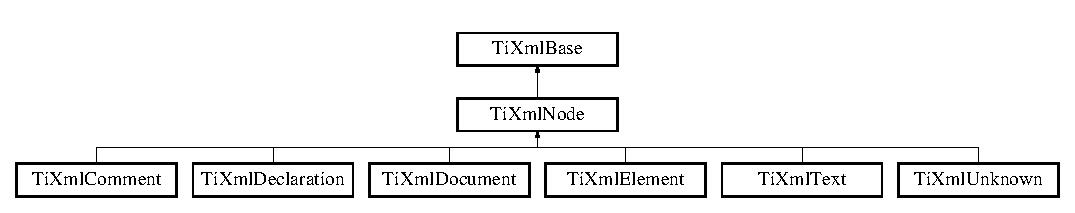
\includegraphics[height=2.413793cm]{class_ti_xml_node}
\end{center}
\end{figure}
\subsection*{Public Types}
\begin{DoxyCompactItemize}
\item 
enum \hyperlink{class_ti_xml_node_a836eded4920ab9e9ef28496f48cd95a2}{NodeType} \{ \par
{\bfseries TINYXML\_\-DOCUMENT}, 
{\bfseries TINYXML\_\-ELEMENT}, 
{\bfseries TINYXML\_\-COMMENT}, 
{\bfseries TINYXML\_\-UNKNOWN}, 
\par
{\bfseries TINYXML\_\-TEXT}, 
{\bfseries TINYXML\_\-DECLARATION}, 
{\bfseries TINYXML\_\-TYPECOUNT}
 \}
\end{DoxyCompactItemize}
\subsection*{Public Member Functions}
\begin{DoxyCompactItemize}
\item 
const char $\ast$ \hyperlink{class_ti_xml_node_a77943eb90d12c2892b1337a9f5918b41}{Value} () const 
\item 
\hypertarget{class_ti_xml_node_a83ece13d2ea66dac66e0b21332229239}{
const TIXML\_\-STRING \& {\bfseries ValueTStr} () const }
\label{class_ti_xml_node_a83ece13d2ea66dac66e0b21332229239}

\item 
void \hyperlink{class_ti_xml_node_a2a38329ca5d3f28f98ce932b8299ae90}{SetValue} (const char $\ast$\_\-value)
\item 
\hypertarget{class_ti_xml_node_a708e7f953df61d4d2d12f73171550a4b}{
void \hyperlink{class_ti_xml_node_a708e7f953df61d4d2d12f73171550a4b}{Clear} ()}
\label{class_ti_xml_node_a708e7f953df61d4d2d12f73171550a4b}

\begin{DoxyCompactList}\small\item\em Delete all the children of this node. Does not affect 'this'. \end{DoxyCompactList}\item 
\hypertarget{class_ti_xml_node_ab643043132ffd794f8602685d34a982e}{
\hyperlink{class_ti_xml_node}{TiXmlNode} $\ast$ \hyperlink{class_ti_xml_node_ab643043132ffd794f8602685d34a982e}{Parent} ()}
\label{class_ti_xml_node_ab643043132ffd794f8602685d34a982e}

\begin{DoxyCompactList}\small\item\em One step up the DOM. \end{DoxyCompactList}\item 
\hypertarget{class_ti_xml_node_a78878709e53066f06eb4fcbcdd3a5260}{
const \hyperlink{class_ti_xml_node}{TiXmlNode} $\ast$ {\bfseries Parent} () const }
\label{class_ti_xml_node_a78878709e53066f06eb4fcbcdd3a5260}

\item 
\hypertarget{class_ti_xml_node_a44c8eee26bbe2d1b2762038df9dde2f0}{
const \hyperlink{class_ti_xml_node}{TiXmlNode} $\ast$ \hyperlink{class_ti_xml_node_a44c8eee26bbe2d1b2762038df9dde2f0}{FirstChild} () const }
\label{class_ti_xml_node_a44c8eee26bbe2d1b2762038df9dde2f0}

\begin{DoxyCompactList}\small\item\em The first child of this node. Will be null if there are no children. \end{DoxyCompactList}\item 
\hypertarget{class_ti_xml_node_a5e97d69b7c0ebd27fb7286be56559b77}{
\hyperlink{class_ti_xml_node}{TiXmlNode} $\ast$ {\bfseries FirstChild} ()}
\label{class_ti_xml_node_a5e97d69b7c0ebd27fb7286be56559b77}

\item 
const \hyperlink{class_ti_xml_node}{TiXmlNode} $\ast$ \hyperlink{class_ti_xml_node_ab5f722624113c8203227de4f56576d31}{FirstChild} (const char $\ast$value) const 
\item 
\hypertarget{class_ti_xml_node_abc8bf32be6419ec453a731868de19554}{
\hyperlink{class_ti_xml_node}{TiXmlNode} $\ast$ \hyperlink{class_ti_xml_node_abc8bf32be6419ec453a731868de19554}{FirstChild} (const char $\ast$\_\-value)}
\label{class_ti_xml_node_abc8bf32be6419ec453a731868de19554}

\begin{DoxyCompactList}\small\item\em The first child of this node with the matching 'value'. Will be null if none found. \end{DoxyCompactList}\item 
\hypertarget{class_ti_xml_node_a6d671107e00cca1d28cb2d7f3a87a21e}{
const \hyperlink{class_ti_xml_node}{TiXmlNode} $\ast$ {\bfseries LastChild} () const }
\label{class_ti_xml_node_a6d671107e00cca1d28cb2d7f3a87a21e}

\item 
\hypertarget{class_ti_xml_node_a6432d2b2495f6caf9cb4278df706a031}{
\hyperlink{class_ti_xml_node}{TiXmlNode} $\ast$ \hyperlink{class_ti_xml_node_a6432d2b2495f6caf9cb4278df706a031}{LastChild} ()}
\label{class_ti_xml_node_a6432d2b2495f6caf9cb4278df706a031}

\begin{DoxyCompactList}\small\item\em The last child of this node. Will be null if there are no children. \end{DoxyCompactList}\item 
\hypertarget{class_ti_xml_node_acdd3fdc436aa7433023310a041e5e63f}{
const \hyperlink{class_ti_xml_node}{TiXmlNode} $\ast$ {\bfseries LastChild} (const char $\ast$value) const }
\label{class_ti_xml_node_acdd3fdc436aa7433023310a041e5e63f}

\item 
\hypertarget{class_ti_xml_node_abad5bf1059c48127b958711ef89e8e5d}{
\hyperlink{class_ti_xml_node}{TiXmlNode} $\ast$ \hyperlink{class_ti_xml_node_abad5bf1059c48127b958711ef89e8e5d}{LastChild} (const char $\ast$\_\-value)}
\label{class_ti_xml_node_abad5bf1059c48127b958711ef89e8e5d}

\begin{DoxyCompactList}\small\item\em The last child of this node matching 'value'. Will be null if there are no children. \end{DoxyCompactList}\item 
const \hyperlink{class_ti_xml_node}{TiXmlNode} $\ast$ \hyperlink{class_ti_xml_node_aaef7ac3978c4bb1cc8a24ffae7bced75}{IterateChildren} (const \hyperlink{class_ti_xml_node}{TiXmlNode} $\ast$previous) const 
\item 
\hypertarget{class_ti_xml_node_a2358e747118fdbf0e467b1e4f7d03de1}{
\hyperlink{class_ti_xml_node}{TiXmlNode} $\ast$ {\bfseries IterateChildren} (const \hyperlink{class_ti_xml_node}{TiXmlNode} $\ast$previous)}
\label{class_ti_xml_node_a2358e747118fdbf0e467b1e4f7d03de1}

\item 
\hypertarget{class_ti_xml_node_af2b86dbe25d3d26fa48180edc5e2a9fc}{
const \hyperlink{class_ti_xml_node}{TiXmlNode} $\ast$ \hyperlink{class_ti_xml_node_af2b86dbe25d3d26fa48180edc5e2a9fc}{IterateChildren} (const char $\ast$value, const \hyperlink{class_ti_xml_node}{TiXmlNode} $\ast$previous) const }
\label{class_ti_xml_node_af2b86dbe25d3d26fa48180edc5e2a9fc}

\begin{DoxyCompactList}\small\item\em This flavor of IterateChildren searches for children with a particular 'value'. \end{DoxyCompactList}\item 
\hypertarget{class_ti_xml_node_a67ba8275e533e6f76340236c42ea0aea}{
\hyperlink{class_ti_xml_node}{TiXmlNode} $\ast$ {\bfseries IterateChildren} (const char $\ast$\_\-value, const \hyperlink{class_ti_xml_node}{TiXmlNode} $\ast$previous)}
\label{class_ti_xml_node_a67ba8275e533e6f76340236c42ea0aea}

\item 
\hyperlink{class_ti_xml_node}{TiXmlNode} $\ast$ \hyperlink{class_ti_xml_node_af287a913ce46d8dbf7ef24fec69bbaf0}{InsertEndChild} (const \hyperlink{class_ti_xml_node}{TiXmlNode} \&addThis)
\item 
\hyperlink{class_ti_xml_node}{TiXmlNode} $\ast$ \hyperlink{class_ti_xml_node_a1a881212554b759865f6cac79a851d38}{LinkEndChild} (\hyperlink{class_ti_xml_node}{TiXmlNode} $\ast$addThis)
\item 
\hyperlink{class_ti_xml_node}{TiXmlNode} $\ast$ \hyperlink{class_ti_xml_node_a71e54e393336382bc9875f64aab5cb15}{InsertBeforeChild} (\hyperlink{class_ti_xml_node}{TiXmlNode} $\ast$beforeThis, const \hyperlink{class_ti_xml_node}{TiXmlNode} \&addThis)
\item 
\hyperlink{class_ti_xml_node}{TiXmlNode} $\ast$ \hyperlink{class_ti_xml_node_a274db3292218202805c093f66a964cb5}{InsertAfterChild} (\hyperlink{class_ti_xml_node}{TiXmlNode} $\ast$afterThis, const \hyperlink{class_ti_xml_node}{TiXmlNode} \&addThis)
\item 
\hyperlink{class_ti_xml_node}{TiXmlNode} $\ast$ \hyperlink{class_ti_xml_node_a543208c2c801c84a213529541e904b9f}{ReplaceChild} (\hyperlink{class_ti_xml_node}{TiXmlNode} $\ast$replaceThis, const \hyperlink{class_ti_xml_node}{TiXmlNode} \&withThis)
\item 
\hypertarget{class_ti_xml_node_ae19d8510efc90596552f4feeac9a8fbf}{
bool \hyperlink{class_ti_xml_node_ae19d8510efc90596552f4feeac9a8fbf}{RemoveChild} (\hyperlink{class_ti_xml_node}{TiXmlNode} $\ast$removeThis)}
\label{class_ti_xml_node_ae19d8510efc90596552f4feeac9a8fbf}

\begin{DoxyCompactList}\small\item\em Delete a child of this node. \end{DoxyCompactList}\item 
\hypertarget{class_ti_xml_node_ac2cd892768726270e511b2ab32de4d10}{
const \hyperlink{class_ti_xml_node}{TiXmlNode} $\ast$ \hyperlink{class_ti_xml_node_ac2cd892768726270e511b2ab32de4d10}{PreviousSibling} () const }
\label{class_ti_xml_node_ac2cd892768726270e511b2ab32de4d10}

\begin{DoxyCompactList}\small\item\em Navigate to a sibling node. \end{DoxyCompactList}\item 
\hypertarget{class_ti_xml_node_af8c0642ad6ecc03f62953e68896ed1cc}{
\hyperlink{class_ti_xml_node}{TiXmlNode} $\ast$ {\bfseries PreviousSibling} ()}
\label{class_ti_xml_node_af8c0642ad6ecc03f62953e68896ed1cc}

\item 
\hypertarget{class_ti_xml_node_abbb3b8c1f38fa7b9e52d584a4aeca795}{
const \hyperlink{class_ti_xml_node}{TiXmlNode} $\ast$ \hyperlink{class_ti_xml_node_abbb3b8c1f38fa7b9e52d584a4aeca795}{PreviousSibling} (const char $\ast$) const }
\label{class_ti_xml_node_abbb3b8c1f38fa7b9e52d584a4aeca795}

\begin{DoxyCompactList}\small\item\em Navigate to a sibling node. \end{DoxyCompactList}\item 
\hypertarget{class_ti_xml_node_a6c977049207177ef21b51972315c2053}{
\hyperlink{class_ti_xml_node}{TiXmlNode} $\ast$ {\bfseries PreviousSibling} (const char $\ast$\_\-prev)}
\label{class_ti_xml_node_a6c977049207177ef21b51972315c2053}

\item 
\hypertarget{class_ti_xml_node_af854baeba384f5fe9859f5aee03b548e}{
const \hyperlink{class_ti_xml_node}{TiXmlNode} $\ast$ \hyperlink{class_ti_xml_node_af854baeba384f5fe9859f5aee03b548e}{NextSibling} () const }
\label{class_ti_xml_node_af854baeba384f5fe9859f5aee03b548e}

\begin{DoxyCompactList}\small\item\em Navigate to a sibling node. \end{DoxyCompactList}\item 
\hypertarget{class_ti_xml_node_a4d05f7b1d7b470ac6887edd072d4892a}{
\hyperlink{class_ti_xml_node}{TiXmlNode} $\ast$ {\bfseries NextSibling} ()}
\label{class_ti_xml_node_a4d05f7b1d7b470ac6887edd072d4892a}

\item 
\hypertarget{class_ti_xml_node_acaf9dc17531ac041f602f9ad579573ea}{
const \hyperlink{class_ti_xml_node}{TiXmlNode} $\ast$ \hyperlink{class_ti_xml_node_acaf9dc17531ac041f602f9ad579573ea}{NextSibling} (const char $\ast$) const }
\label{class_ti_xml_node_acaf9dc17531ac041f602f9ad579573ea}

\begin{DoxyCompactList}\small\item\em Navigate to a sibling node with the given 'value'. \end{DoxyCompactList}\item 
\hypertarget{class_ti_xml_node_a4080bc5cc8a5c139e7cf308669e850fc}{
\hyperlink{class_ti_xml_node}{TiXmlNode} $\ast$ {\bfseries NextSibling} (const char $\ast$\_\-next)}
\label{class_ti_xml_node_a4080bc5cc8a5c139e7cf308669e850fc}

\item 
const \hyperlink{class_ti_xml_element}{TiXmlElement} $\ast$ \hyperlink{class_ti_xml_node_a7667217e269e0da01d1f82aee94d1a3d}{NextSiblingElement} () const 
\item 
\hypertarget{class_ti_xml_node_a1b211cb5034655a04358e0e2f6fc5010}{
\hyperlink{class_ti_xml_element}{TiXmlElement} $\ast$ {\bfseries NextSiblingElement} ()}
\label{class_ti_xml_node_a1b211cb5034655a04358e0e2f6fc5010}

\item 
const \hyperlink{class_ti_xml_element}{TiXmlElement} $\ast$ \hyperlink{class_ti_xml_node_a3d7897999f99cf4870dd59df6331d7ff}{NextSiblingElement} (const char $\ast$) const 
\item 
\hypertarget{class_ti_xml_node_a6e1ac6b800e18049bc75e9f8e63a8e5f}{
\hyperlink{class_ti_xml_element}{TiXmlElement} $\ast$ {\bfseries NextSiblingElement} (const char $\ast$\_\-next)}
\label{class_ti_xml_node_a6e1ac6b800e18049bc75e9f8e63a8e5f}

\item 
\hypertarget{class_ti_xml_node_ab1f8d8e70d88aea4c5efedfe00862d55}{
const \hyperlink{class_ti_xml_element}{TiXmlElement} $\ast$ \hyperlink{class_ti_xml_node_ab1f8d8e70d88aea4c5efedfe00862d55}{FirstChildElement} () const }
\label{class_ti_xml_node_ab1f8d8e70d88aea4c5efedfe00862d55}

\begin{DoxyCompactList}\small\item\em Convenience function to get through elements. \end{DoxyCompactList}\item 
\hypertarget{class_ti_xml_node_aa0fecff1f3866ab33a8a25506e95db1d}{
\hyperlink{class_ti_xml_element}{TiXmlElement} $\ast$ {\bfseries FirstChildElement} ()}
\label{class_ti_xml_node_aa0fecff1f3866ab33a8a25506e95db1d}

\item 
\hypertarget{class_ti_xml_node_a0ec361bfef1cf1978d060295f597e0d9}{
const \hyperlink{class_ti_xml_element}{TiXmlElement} $\ast$ \hyperlink{class_ti_xml_node_a0ec361bfef1cf1978d060295f597e0d9}{FirstChildElement} (const char $\ast$\_\-value) const }
\label{class_ti_xml_node_a0ec361bfef1cf1978d060295f597e0d9}

\begin{DoxyCompactList}\small\item\em Convenience function to get through elements. \end{DoxyCompactList}\item 
\hypertarget{class_ti_xml_node_a6936ae323675071808ac4840379e57f5}{
\hyperlink{class_ti_xml_element}{TiXmlElement} $\ast$ {\bfseries FirstChildElement} (const char $\ast$\_\-value)}
\label{class_ti_xml_node_a6936ae323675071808ac4840379e57f5}

\item 
int \hyperlink{class_ti_xml_node_a57b99d5c97d67a42b9752f5210a1ba5e}{Type} () const 
\item 
const \hyperlink{class_ti_xml_document}{TiXmlDocument} $\ast$ \hyperlink{class_ti_xml_node_aa66f4ebcd175204a168ed7c2d7b43071}{GetDocument} () const 
\item 
\hypertarget{class_ti_xml_node_a7b2372c0e7adfb32f5b6902fe49a39b2}{
\hyperlink{class_ti_xml_document}{TiXmlDocument} $\ast$ {\bfseries GetDocument} ()}
\label{class_ti_xml_node_a7b2372c0e7adfb32f5b6902fe49a39b2}

\item 
\hypertarget{class_ti_xml_node_aeed21ad30630ef6e7faf096127edc9f3}{
bool \hyperlink{class_ti_xml_node_aeed21ad30630ef6e7faf096127edc9f3}{NoChildren} () const }
\label{class_ti_xml_node_aeed21ad30630ef6e7faf096127edc9f3}

\begin{DoxyCompactList}\small\item\em Returns true if this node has no children. \end{DoxyCompactList}\item 
\hypertarget{class_ti_xml_node_a8a4cda4b15c29f64cff419309aebed08}{
virtual const \hyperlink{class_ti_xml_document}{TiXmlDocument} $\ast$ \hyperlink{class_ti_xml_node_a8a4cda4b15c29f64cff419309aebed08}{ToDocument} () const }
\label{class_ti_xml_node_a8a4cda4b15c29f64cff419309aebed08}

\begin{DoxyCompactList}\small\item\em Cast to a more defined type. Will return null if not of the requested type. \end{DoxyCompactList}\item 
\hypertarget{class_ti_xml_node_a72abed96dc9667ab9e0a2a275301bb1c}{
virtual const \hyperlink{class_ti_xml_element}{TiXmlElement} $\ast$ \hyperlink{class_ti_xml_node_a72abed96dc9667ab9e0a2a275301bb1c}{ToElement} () const }
\label{class_ti_xml_node_a72abed96dc9667ab9e0a2a275301bb1c}

\begin{DoxyCompactList}\small\item\em Cast to a more defined type. Will return null if not of the requested type. \end{DoxyCompactList}\item 
\hypertarget{class_ti_xml_node_aa0a5086f9eaee910bbfdc7f975e26574}{
virtual const \hyperlink{class_ti_xml_comment}{TiXmlComment} $\ast$ \hyperlink{class_ti_xml_node_aa0a5086f9eaee910bbfdc7f975e26574}{ToComment} () const }
\label{class_ti_xml_node_aa0a5086f9eaee910bbfdc7f975e26574}

\begin{DoxyCompactList}\small\item\em Cast to a more defined type. Will return null if not of the requested type. \end{DoxyCompactList}\item 
\hypertarget{class_ti_xml_node_afd7205cf31d7a376929f8a36930627a2}{
virtual const \hyperlink{class_ti_xml_unknown}{TiXmlUnknown} $\ast$ \hyperlink{class_ti_xml_node_afd7205cf31d7a376929f8a36930627a2}{ToUnknown} () const }
\label{class_ti_xml_node_afd7205cf31d7a376929f8a36930627a2}

\begin{DoxyCompactList}\small\item\em Cast to a more defined type. Will return null if not of the requested type. \end{DoxyCompactList}\item 
\hypertarget{class_ti_xml_node_a95a46a52c525992d6b4ee08beb14cd69}{
virtual const \hyperlink{class_ti_xml_text}{TiXmlText} $\ast$ \hyperlink{class_ti_xml_node_a95a46a52c525992d6b4ee08beb14cd69}{ToText} () const }
\label{class_ti_xml_node_a95a46a52c525992d6b4ee08beb14cd69}

\begin{DoxyCompactList}\small\item\em Cast to a more defined type. Will return null if not of the requested type. \end{DoxyCompactList}\item 
\hypertarget{class_ti_xml_node_a9f43e6984fc7d4afd6eb32714c6b7b72}{
virtual const \hyperlink{class_ti_xml_declaration}{TiXmlDeclaration} $\ast$ \hyperlink{class_ti_xml_node_a9f43e6984fc7d4afd6eb32714c6b7b72}{ToDeclaration} () const }
\label{class_ti_xml_node_a9f43e6984fc7d4afd6eb32714c6b7b72}

\begin{DoxyCompactList}\small\item\em Cast to a more defined type. Will return null if not of the requested type. \end{DoxyCompactList}\item 
\hypertarget{class_ti_xml_node_a6a4c8ac28ee7a745d059db6691e03bae}{
virtual \hyperlink{class_ti_xml_document}{TiXmlDocument} $\ast$ \hyperlink{class_ti_xml_node_a6a4c8ac28ee7a745d059db6691e03bae}{ToDocument} ()}
\label{class_ti_xml_node_a6a4c8ac28ee7a745d059db6691e03bae}

\begin{DoxyCompactList}\small\item\em Cast to a more defined type. Will return null if not of the requested type. \end{DoxyCompactList}\item 
\hypertarget{class_ti_xml_node_aa65d000223187d22a4dcebd7479e9ebc}{
virtual \hyperlink{class_ti_xml_element}{TiXmlElement} $\ast$ \hyperlink{class_ti_xml_node_aa65d000223187d22a4dcebd7479e9ebc}{ToElement} ()}
\label{class_ti_xml_node_aa65d000223187d22a4dcebd7479e9ebc}

\begin{DoxyCompactList}\small\item\em Cast to a more defined type. Will return null if not of the requested type. \end{DoxyCompactList}\item 
\hypertarget{class_ti_xml_node_a383e06a0787f7063953934867990f849}{
virtual \hyperlink{class_ti_xml_comment}{TiXmlComment} $\ast$ \hyperlink{class_ti_xml_node_a383e06a0787f7063953934867990f849}{ToComment} ()}
\label{class_ti_xml_node_a383e06a0787f7063953934867990f849}

\begin{DoxyCompactList}\small\item\em Cast to a more defined type. Will return null if not of the requested type. \end{DoxyCompactList}\item 
\hypertarget{class_ti_xml_node_a06de5af852668c7e4af0d09c205f0b0d}{
virtual \hyperlink{class_ti_xml_unknown}{TiXmlUnknown} $\ast$ \hyperlink{class_ti_xml_node_a06de5af852668c7e4af0d09c205f0b0d}{ToUnknown} ()}
\label{class_ti_xml_node_a06de5af852668c7e4af0d09c205f0b0d}

\begin{DoxyCompactList}\small\item\em Cast to a more defined type. Will return null if not of the requested type. \end{DoxyCompactList}\item 
\hypertarget{class_ti_xml_node_a3ddfbcac78fbea041fad57e5c6d60a03}{
virtual \hyperlink{class_ti_xml_text}{TiXmlText} $\ast$ \hyperlink{class_ti_xml_node_a3ddfbcac78fbea041fad57e5c6d60a03}{ToText} ()}
\label{class_ti_xml_node_a3ddfbcac78fbea041fad57e5c6d60a03}

\begin{DoxyCompactList}\small\item\em Cast to a more defined type. Will return null if not of the requested type. \end{DoxyCompactList}\item 
\hypertarget{class_ti_xml_node_a4027136ca820ff4a636b607231b6a6df}{
virtual \hyperlink{class_ti_xml_declaration}{TiXmlDeclaration} $\ast$ \hyperlink{class_ti_xml_node_a4027136ca820ff4a636b607231b6a6df}{ToDeclaration} ()}
\label{class_ti_xml_node_a4027136ca820ff4a636b607231b6a6df}

\begin{DoxyCompactList}\small\item\em Cast to a more defined type. Will return null if not of the requested type. \end{DoxyCompactList}\item 
virtual \hyperlink{class_ti_xml_node}{TiXmlNode} $\ast$ \hyperlink{class_ti_xml_node_a4508cc3a2d7a98e96a54cc09c37a78a4}{Clone} () const =0
\item 
virtual bool \hyperlink{class_ti_xml_node_acc0f88b7462c6cb73809d410a4f5bb86}{Accept} (\hyperlink{class_ti_xml_visitor}{TiXmlVisitor} $\ast$visitor) const =0
\end{DoxyCompactItemize}
\subsection*{Protected Member Functions}
\begin{DoxyCompactItemize}
\item 
\hypertarget{class_ti_xml_node_a3f46721695868667113c7487ff123f20}{
{\bfseries TiXmlNode} (\hyperlink{class_ti_xml_node_a836eded4920ab9e9ef28496f48cd95a2}{NodeType} \_\-type)}
\label{class_ti_xml_node_a3f46721695868667113c7487ff123f20}

\item 
\hypertarget{class_ti_xml_node_ab6056978923ad8350fb5164af32d8038}{
void {\bfseries CopyTo} (\hyperlink{class_ti_xml_node}{TiXmlNode} $\ast$target) const }
\label{class_ti_xml_node_ab6056978923ad8350fb5164af32d8038}

\item 
\hypertarget{class_ti_xml_node_ac1e3a8e7578be463b04617786120c2bb}{
\hyperlink{class_ti_xml_node}{TiXmlNode} $\ast$ {\bfseries Identify} (const char $\ast$start, TiXmlEncoding encoding)}
\label{class_ti_xml_node_ac1e3a8e7578be463b04617786120c2bb}

\end{DoxyCompactItemize}
\subsection*{Protected Attributes}
\begin{DoxyCompactItemize}
\item 
\hypertarget{class_ti_xml_node_a662c4de61244e4fa5bd4e2d8c63143a5}{
\hyperlink{class_ti_xml_node}{TiXmlNode} $\ast$ {\bfseries parent}}
\label{class_ti_xml_node_a662c4de61244e4fa5bd4e2d8c63143a5}

\item 
\hypertarget{class_ti_xml_node_a2619c6379181c16ba95ae6922e2ca839}{
\hyperlink{class_ti_xml_node_a836eded4920ab9e9ef28496f48cd95a2}{NodeType} {\bfseries type}}
\label{class_ti_xml_node_a2619c6379181c16ba95ae6922e2ca839}

\item 
\hypertarget{class_ti_xml_node_af749fb7f22010b80e8f904c32653d50e}{
\hyperlink{class_ti_xml_node}{TiXmlNode} $\ast$ {\bfseries firstChild}}
\label{class_ti_xml_node_af749fb7f22010b80e8f904c32653d50e}

\item 
\hypertarget{class_ti_xml_node_a5b30756d21b304580d22a841ec9d61f8}{
\hyperlink{class_ti_xml_node}{TiXmlNode} $\ast$ {\bfseries lastChild}}
\label{class_ti_xml_node_a5b30756d21b304580d22a841ec9d61f8}

\item 
\hypertarget{class_ti_xml_node_aead528b3cedc33c16a6c539872c7cc8b}{
TIXML\_\-STRING {\bfseries value}}
\label{class_ti_xml_node_aead528b3cedc33c16a6c539872c7cc8b}

\item 
\hypertarget{class_ti_xml_node_a9c5370ea2cbfd9f0e0f7b30a57fd68f5}{
\hyperlink{class_ti_xml_node}{TiXmlNode} $\ast$ {\bfseries prev}}
\label{class_ti_xml_node_a9c5370ea2cbfd9f0e0f7b30a57fd68f5}

\item 
\hypertarget{class_ti_xml_node_a2f329cc993d2d34df76e17dcbb776b45}{
\hyperlink{class_ti_xml_node}{TiXmlNode} $\ast$ {\bfseries next}}
\label{class_ti_xml_node_a2f329cc993d2d34df76e17dcbb776b45}

\end{DoxyCompactItemize}
\subsection*{Friends}
\begin{DoxyCompactItemize}
\item 
\hypertarget{class_ti_xml_node_a173617f6dfe902cf484ce5552b950475}{
class \hyperlink{class_ti_xml_node_a173617f6dfe902cf484ce5552b950475}{TiXmlDocument}}
\label{class_ti_xml_node_a173617f6dfe902cf484ce5552b950475}

\item 
\hypertarget{class_ti_xml_node_ab6592e32cb9132be517cc12a70564c4b}{
class \hyperlink{class_ti_xml_node_ab6592e32cb9132be517cc12a70564c4b}{TiXmlElement}}
\label{class_ti_xml_node_ab6592e32cb9132be517cc12a70564c4b}

\end{DoxyCompactItemize}


\subsection{Detailed Description}
The parent class for everything in the Document Object Model. (Except for attributes). Nodes have siblings, a parent, and children. A node can be in a document, or stand on its own. The type of a \hyperlink{class_ti_xml_node}{TiXmlNode} can be queried, and it can be cast to its more defined type. 

\subsection{Member Enumeration Documentation}
\hypertarget{class_ti_xml_node_a836eded4920ab9e9ef28496f48cd95a2}{
\index{TiXmlNode@{TiXmlNode}!NodeType@{NodeType}}
\index{NodeType@{NodeType}!TiXmlNode@{TiXmlNode}}
\subsubsection[{NodeType}]{\setlength{\rightskip}{0pt plus 5cm}enum {\bf TiXmlNode::NodeType}}}
\label{class_ti_xml_node_a836eded4920ab9e9ef28496f48cd95a2}
The types of XML nodes supported by TinyXml. (All the unsupported types are picked up by UNKNOWN.) 

\subsection{Member Function Documentation}
\hypertarget{class_ti_xml_node_acc0f88b7462c6cb73809d410a4f5bb86}{
\index{TiXmlNode@{TiXmlNode}!Accept@{Accept}}
\index{Accept@{Accept}!TiXmlNode@{TiXmlNode}}
\subsubsection[{Accept}]{\setlength{\rightskip}{0pt plus 5cm}virtual bool TiXmlNode::Accept (
\begin{DoxyParamCaption}
\item[{{\bf TiXmlVisitor} $\ast$}]{visitor}
\end{DoxyParamCaption}
) const\hspace{0.3cm}{\ttfamily  \mbox{[}pure virtual\mbox{]}}}}
\label{class_ti_xml_node_acc0f88b7462c6cb73809d410a4f5bb86}
Accept a hierchical visit the nodes in the TinyXML DOM. Every node in the XML tree will be conditionally visited and the host will be called back via the \hyperlink{class_ti_xml_visitor}{TiXmlVisitor} interface.

This is essentially a SAX interface for TinyXML. (Note however it doesn't re-\/parse the XML for the callbacks, so the performance of TinyXML is unchanged by using this interface versus any other.)

The interface has been based on ideas from:


\begin{DoxyItemize}
\item \href{http://www.saxproject.org/}{\tt http://www.saxproject.org/}
\item \href{http://c2.com/cgi/wiki?HierarchicalVisitorPattern}{\tt http://c2.com/cgi/wiki?HierarchicalVisitorPattern}
\end{DoxyItemize}

Which are both good references for \char`\"{}visiting\char`\"{}.

An example of using \hyperlink{class_ti_xml_node_acc0f88b7462c6cb73809d410a4f5bb86}{Accept()}: \begin{DoxyVerb}
		TiXmlPrinter printer;
		tinyxmlDoc.Accept( &printer );
		const char* xmlcstr = printer.CStr();
		\end{DoxyVerb}
 

Implemented in \hyperlink{class_ti_xml_element_a31ab28cc3b892a69254391d6bbe08df3}{TiXmlElement}, \hyperlink{class_ti_xml_comment_a4382de0e50da973f11a23ea5852568bd}{TiXmlComment}, \hyperlink{class_ti_xml_text_a43b9954ebf679557fac1a4453f337b7c}{TiXmlText}, \hyperlink{class_ti_xml_declaration_ab6a6b178161ba9abc2c35058de689864}{TiXmlDeclaration}, \hyperlink{class_ti_xml_unknown_a4e54d7482e05a837cf83c925cc683380}{TiXmlUnknown}, and \hyperlink{class_ti_xml_document_a3daab2f472418ef66315750202f762ae}{TiXmlDocument}.

\hypertarget{class_ti_xml_node_a4508cc3a2d7a98e96a54cc09c37a78a4}{
\index{TiXmlNode@{TiXmlNode}!Clone@{Clone}}
\index{Clone@{Clone}!TiXmlNode@{TiXmlNode}}
\subsubsection[{Clone}]{\setlength{\rightskip}{0pt plus 5cm}virtual {\bf TiXmlNode}$\ast$ TiXmlNode::Clone (
\begin{DoxyParamCaption}
{}
\end{DoxyParamCaption}
) const\hspace{0.3cm}{\ttfamily  \mbox{[}pure virtual\mbox{]}}}}
\label{class_ti_xml_node_a4508cc3a2d7a98e96a54cc09c37a78a4}
Create an exact duplicate of this node and return it. The memory must be deleted by the caller. 

Implemented in \hyperlink{class_ti_xml_element_a13f6df105ebb1e8dc636e75cc883be32}{TiXmlElement}, \hyperlink{class_ti_xml_comment_a4f6590c9c9a2b63a48972655b78eb853}{TiXmlComment}, \hyperlink{class_ti_xml_text_adde1869dfb029be50713fbfd8ce4d21f}{TiXmlText}, \hyperlink{class_ti_xml_declaration_aff8231266d735943d8a7514a9c9822b9}{TiXmlDeclaration}, \hyperlink{class_ti_xml_unknown_a675c4b2684af35e4c7649b7fd5ae598d}{TiXmlUnknown}, and \hyperlink{class_ti_xml_document_ac9e8f09b23454d953b32d1b65cd1409e}{TiXmlDocument}.

\hypertarget{class_ti_xml_node_ab5f722624113c8203227de4f56576d31}{
\index{TiXmlNode@{TiXmlNode}!FirstChild@{FirstChild}}
\index{FirstChild@{FirstChild}!TiXmlNode@{TiXmlNode}}
\subsubsection[{FirstChild}]{\setlength{\rightskip}{0pt plus 5cm}const {\bf TiXmlNode} $\ast$ TiXmlNode::FirstChild (
\begin{DoxyParamCaption}
\item[{const char $\ast$}]{value}
\end{DoxyParamCaption}
) const}}
\label{class_ti_xml_node_ab5f722624113c8203227de4f56576d31}
The first child of this node with the matching 'value'. Will be null if none found. \hypertarget{class_ti_xml_node_aa66f4ebcd175204a168ed7c2d7b43071}{
\index{TiXmlNode@{TiXmlNode}!GetDocument@{GetDocument}}
\index{GetDocument@{GetDocument}!TiXmlNode@{TiXmlNode}}
\subsubsection[{GetDocument}]{\setlength{\rightskip}{0pt plus 5cm}const {\bf TiXmlDocument} $\ast$ TiXmlNode::GetDocument (
\begin{DoxyParamCaption}
{}
\end{DoxyParamCaption}
) const}}
\label{class_ti_xml_node_aa66f4ebcd175204a168ed7c2d7b43071}
Return a pointer to the Document this node lives in. Returns null if not in a document. \hypertarget{class_ti_xml_node_a274db3292218202805c093f66a964cb5}{
\index{TiXmlNode@{TiXmlNode}!InsertAfterChild@{InsertAfterChild}}
\index{InsertAfterChild@{InsertAfterChild}!TiXmlNode@{TiXmlNode}}
\subsubsection[{InsertAfterChild}]{\setlength{\rightskip}{0pt plus 5cm}{\bf TiXmlNode} $\ast$ TiXmlNode::InsertAfterChild (
\begin{DoxyParamCaption}
\item[{{\bf TiXmlNode} $\ast$}]{afterThis, }
\item[{const {\bf TiXmlNode} \&}]{addThis}
\end{DoxyParamCaption}
)}}
\label{class_ti_xml_node_a274db3292218202805c093f66a964cb5}
Add a new node related to this. Adds a child after the specified child. Returns a pointer to the new object or NULL if an error occured. \hypertarget{class_ti_xml_node_a71e54e393336382bc9875f64aab5cb15}{
\index{TiXmlNode@{TiXmlNode}!InsertBeforeChild@{InsertBeforeChild}}
\index{InsertBeforeChild@{InsertBeforeChild}!TiXmlNode@{TiXmlNode}}
\subsubsection[{InsertBeforeChild}]{\setlength{\rightskip}{0pt plus 5cm}{\bf TiXmlNode} $\ast$ TiXmlNode::InsertBeforeChild (
\begin{DoxyParamCaption}
\item[{{\bf TiXmlNode} $\ast$}]{beforeThis, }
\item[{const {\bf TiXmlNode} \&}]{addThis}
\end{DoxyParamCaption}
)}}
\label{class_ti_xml_node_a71e54e393336382bc9875f64aab5cb15}
Add a new node related to this. Adds a child before the specified child. Returns a pointer to the new object or NULL if an error occured. \hypertarget{class_ti_xml_node_af287a913ce46d8dbf7ef24fec69bbaf0}{
\index{TiXmlNode@{TiXmlNode}!InsertEndChild@{InsertEndChild}}
\index{InsertEndChild@{InsertEndChild}!TiXmlNode@{TiXmlNode}}
\subsubsection[{InsertEndChild}]{\setlength{\rightskip}{0pt plus 5cm}{\bf TiXmlNode} $\ast$ TiXmlNode::InsertEndChild (
\begin{DoxyParamCaption}
\item[{const {\bf TiXmlNode} \&}]{addThis}
\end{DoxyParamCaption}
)}}
\label{class_ti_xml_node_af287a913ce46d8dbf7ef24fec69bbaf0}
Add a new node related to this. Adds a child past the LastChild. Returns a pointer to the new object or NULL if an error occured. \hypertarget{class_ti_xml_node_aaef7ac3978c4bb1cc8a24ffae7bced75}{
\index{TiXmlNode@{TiXmlNode}!IterateChildren@{IterateChildren}}
\index{IterateChildren@{IterateChildren}!TiXmlNode@{TiXmlNode}}
\subsubsection[{IterateChildren}]{\setlength{\rightskip}{0pt plus 5cm}const {\bf TiXmlNode} $\ast$ TiXmlNode::IterateChildren (
\begin{DoxyParamCaption}
\item[{const {\bf TiXmlNode} $\ast$}]{previous}
\end{DoxyParamCaption}
) const}}
\label{class_ti_xml_node_aaef7ac3978c4bb1cc8a24ffae7bced75}
An alternate way to walk the children of a node. One way to iterate over nodes is: \begin{DoxyVerb}
			for( child = parent->FirstChild(); child; child = child->NextSibling() )
		\end{DoxyVerb}


IterateChildren does the same thing with the syntax: \begin{DoxyVerb}
			child = 0;
			while( child = parent->IterateChildren( child ) )
		\end{DoxyVerb}


IterateChildren takes the previous child as input and finds the next one. If the previous child is null, it returns the first. IterateChildren will return null when done. \hypertarget{class_ti_xml_node_a1a881212554b759865f6cac79a851d38}{
\index{TiXmlNode@{TiXmlNode}!LinkEndChild@{LinkEndChild}}
\index{LinkEndChild@{LinkEndChild}!TiXmlNode@{TiXmlNode}}
\subsubsection[{LinkEndChild}]{\setlength{\rightskip}{0pt plus 5cm}{\bf TiXmlNode} $\ast$ TiXmlNode::LinkEndChild (
\begin{DoxyParamCaption}
\item[{{\bf TiXmlNode} $\ast$}]{addThis}
\end{DoxyParamCaption}
)}}
\label{class_ti_xml_node_a1a881212554b759865f6cac79a851d38}
Add a new node related to this. Adds a child past the LastChild.

NOTE: the node to be added is passed by pointer, and will be henceforth owned (and deleted) by tinyXml. This method is efficient and avoids an extra copy, but should be used with care as it uses a different memory model than the other insert functions.

\begin{DoxySeeAlso}{See also}
\hyperlink{class_ti_xml_node_af287a913ce46d8dbf7ef24fec69bbaf0}{InsertEndChild} 
\end{DoxySeeAlso}
\hypertarget{class_ti_xml_node_a3d7897999f99cf4870dd59df6331d7ff}{
\index{TiXmlNode@{TiXmlNode}!NextSiblingElement@{NextSiblingElement}}
\index{NextSiblingElement@{NextSiblingElement}!TiXmlNode@{TiXmlNode}}
\subsubsection[{NextSiblingElement}]{\setlength{\rightskip}{0pt plus 5cm}const {\bf TiXmlElement} $\ast$ TiXmlNode::NextSiblingElement (
\begin{DoxyParamCaption}
\item[{const char $\ast$}]{\_\-value}
\end{DoxyParamCaption}
) const}}
\label{class_ti_xml_node_a3d7897999f99cf4870dd59df6331d7ff}
Convenience function to get through elements. Calls NextSibling and ToElement. Will skip all non-\/Element nodes. Returns 0 if there is not another element. \hypertarget{class_ti_xml_node_a7667217e269e0da01d1f82aee94d1a3d}{
\index{TiXmlNode@{TiXmlNode}!NextSiblingElement@{NextSiblingElement}}
\index{NextSiblingElement@{NextSiblingElement}!TiXmlNode@{TiXmlNode}}
\subsubsection[{NextSiblingElement}]{\setlength{\rightskip}{0pt plus 5cm}const {\bf TiXmlElement} $\ast$ TiXmlNode::NextSiblingElement (
\begin{DoxyParamCaption}
{}
\end{DoxyParamCaption}
) const}}
\label{class_ti_xml_node_a7667217e269e0da01d1f82aee94d1a3d}
Convenience function to get through elements. Calls NextSibling and ToElement. Will skip all non-\/Element nodes. Returns 0 if there is not another element. \hypertarget{class_ti_xml_node_a543208c2c801c84a213529541e904b9f}{
\index{TiXmlNode@{TiXmlNode}!ReplaceChild@{ReplaceChild}}
\index{ReplaceChild@{ReplaceChild}!TiXmlNode@{TiXmlNode}}
\subsubsection[{ReplaceChild}]{\setlength{\rightskip}{0pt plus 5cm}{\bf TiXmlNode} $\ast$ TiXmlNode::ReplaceChild (
\begin{DoxyParamCaption}
\item[{{\bf TiXmlNode} $\ast$}]{replaceThis, }
\item[{const {\bf TiXmlNode} \&}]{withThis}
\end{DoxyParamCaption}
)}}
\label{class_ti_xml_node_a543208c2c801c84a213529541e904b9f}
Replace a child of this node. Returns a pointer to the new object or NULL if an error occured. \hypertarget{class_ti_xml_node_a2a38329ca5d3f28f98ce932b8299ae90}{
\index{TiXmlNode@{TiXmlNode}!SetValue@{SetValue}}
\index{SetValue@{SetValue}!TiXmlNode@{TiXmlNode}}
\subsubsection[{SetValue}]{\setlength{\rightskip}{0pt plus 5cm}void TiXmlNode::SetValue (
\begin{DoxyParamCaption}
\item[{const char $\ast$}]{\_\-value}
\end{DoxyParamCaption}
)\hspace{0.3cm}{\ttfamily  \mbox{[}inline\mbox{]}}}}
\label{class_ti_xml_node_a2a38329ca5d3f28f98ce932b8299ae90}
Changes the value of the node. Defined as: \begin{DoxyVerb}
		Document:	filename of the xml file
		Element:	name of the element
		Comment:	the comment text
		Unknown:	the tag contents
		Text:		the text string
		\end{DoxyVerb}
 \hypertarget{class_ti_xml_node_a57b99d5c97d67a42b9752f5210a1ba5e}{
\index{TiXmlNode@{TiXmlNode}!Type@{Type}}
\index{Type@{Type}!TiXmlNode@{TiXmlNode}}
\subsubsection[{Type}]{\setlength{\rightskip}{0pt plus 5cm}int TiXmlNode::Type (
\begin{DoxyParamCaption}
{}
\end{DoxyParamCaption}
) const\hspace{0.3cm}{\ttfamily  \mbox{[}inline\mbox{]}}}}
\label{class_ti_xml_node_a57b99d5c97d67a42b9752f5210a1ba5e}
Query the type (as an enumerated value, above) of this node. The possible types are: TINYXML\_\-DOCUMENT, TINYXML\_\-ELEMENT, TINYXML\_\-COMMENT, TINYXML\_\-UNKNOWN, TINYXML\_\-TEXT, and TINYXML\_\-DECLARATION. \hypertarget{class_ti_xml_node_a77943eb90d12c2892b1337a9f5918b41}{
\index{TiXmlNode@{TiXmlNode}!Value@{Value}}
\index{Value@{Value}!TiXmlNode@{TiXmlNode}}
\subsubsection[{Value}]{\setlength{\rightskip}{0pt plus 5cm}const char$\ast$ TiXmlNode::Value (
\begin{DoxyParamCaption}
{}
\end{DoxyParamCaption}
) const\hspace{0.3cm}{\ttfamily  \mbox{[}inline\mbox{]}}}}
\label{class_ti_xml_node_a77943eb90d12c2892b1337a9f5918b41}
The meaning of 'value' changes for the specific type of \hyperlink{class_ti_xml_node}{TiXmlNode}. \begin{DoxyVerb}
		Document:	filename of the xml file
		Element:	name of the element
		Comment:	the comment text
		Unknown:	the tag contents
		Text:		the text string
		\end{DoxyVerb}


The subclasses will wrap this function. 

The documentation for this class was generated from the following files:\begin{DoxyCompactItemize}
\item 
/home/cshome/m/mabrams/345/txtEngine/tinyxml.h\item 
/home/cshome/m/mabrams/345/txtEngine/tinyxml.cpp\item 
/home/cshome/m/mabrams/345/txtEngine/tinyxmlparser.cpp\end{DoxyCompactItemize}

\hypertarget{class_ti_xml_out_stream}{
\section{\-Ti\-Xml\-Out\-Stream \-Class \-Reference}
\label{class_ti_xml_out_stream}\index{\-Ti\-Xml\-Out\-Stream@{\-Ti\-Xml\-Out\-Stream}}
}
\-Inheritance diagram for \-Ti\-Xml\-Out\-Stream\-:\begin{figure}[H]
\begin{center}
\leavevmode
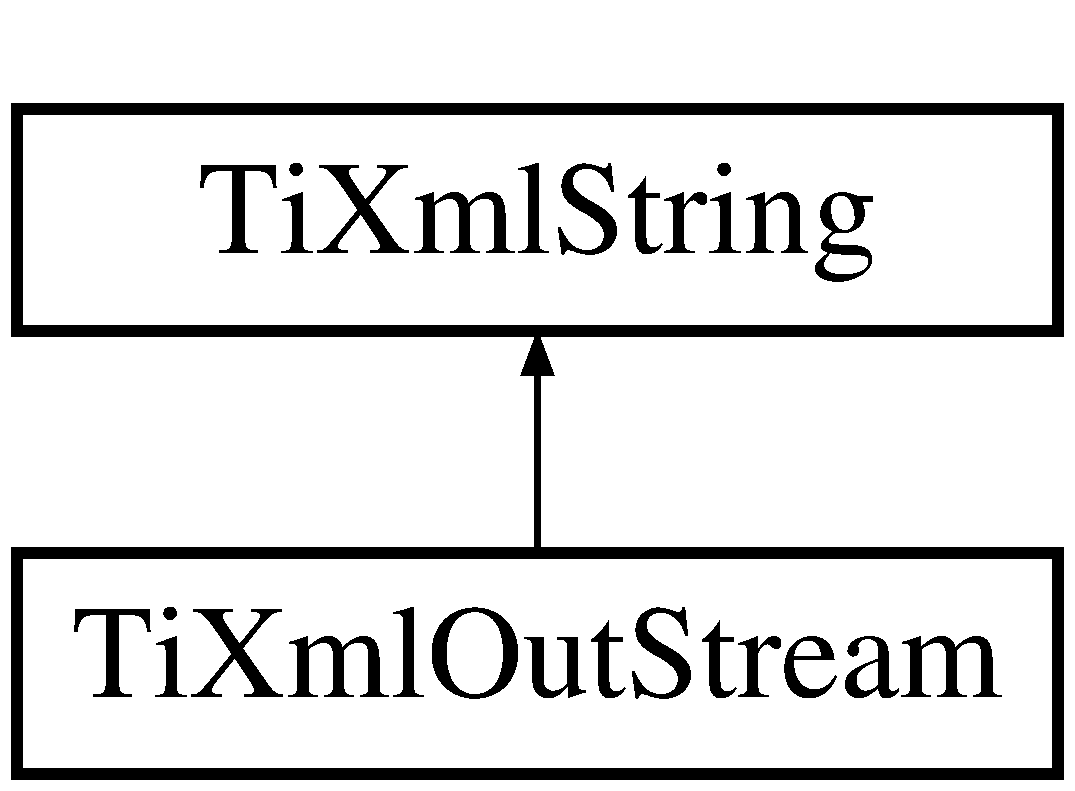
\includegraphics[height=2.000000cm]{class_ti_xml_out_stream}
\end{center}
\end{figure}
\subsection*{\-Public \-Member \-Functions}
\begin{DoxyCompactItemize}
\item 
\hypertarget{class_ti_xml_out_stream_a3640dcb1c0903be3bc6966cdc9a79db6}{
\hyperlink{class_ti_xml_out_stream}{\-Ti\-Xml\-Out\-Stream} \& {\bfseries operator$<$$<$} (const \hyperlink{class_ti_xml_string}{\-Ti\-Xml\-String} \&in)}
\label{class_ti_xml_out_stream_a3640dcb1c0903be3bc6966cdc9a79db6}

\item 
\hypertarget{class_ti_xml_out_stream_af2117e5a8cbfcb69544804ad2859bfb6}{
\hyperlink{class_ti_xml_out_stream}{\-Ti\-Xml\-Out\-Stream} \& {\bfseries operator$<$$<$} (const char $\ast$in)}
\label{class_ti_xml_out_stream_af2117e5a8cbfcb69544804ad2859bfb6}

\end{DoxyCompactItemize}


\-The documentation for this class was generated from the following file\-:\begin{DoxyCompactItemize}
\item 
/home/cshome/m/mabrams/345/txt\-Engine/tinystr.\-h\end{DoxyCompactItemize}

\hypertarget{class_ti_xml_parsing_data}{
\section{TiXmlParsingData Class Reference}
\label{class_ti_xml_parsing_data}\index{TiXmlParsingData@{TiXmlParsingData}}
}
\subsection*{Public Member Functions}
\begin{DoxyCompactItemize}
\item 
\hypertarget{class_ti_xml_parsing_data_a65cee8ab77a36c605db08c84b4c30a7d}{
void {\bfseries Stamp} (const char $\ast$now, TiXmlEncoding encoding)}
\label{class_ti_xml_parsing_data_a65cee8ab77a36c605db08c84b4c30a7d}

\item 
\hypertarget{class_ti_xml_parsing_data_a9e63d965fdb53ff4ac711e105269e918}{
const \hyperlink{struct_ti_xml_cursor}{TiXmlCursor} \& {\bfseries Cursor} () const }
\label{class_ti_xml_parsing_data_a9e63d965fdb53ff4ac711e105269e918}

\end{DoxyCompactItemize}
\subsection*{Friends}
\begin{DoxyCompactItemize}
\item 
\hypertarget{class_ti_xml_parsing_data_a173617f6dfe902cf484ce5552b950475}{
class \hyperlink{class_ti_xml_parsing_data_a173617f6dfe902cf484ce5552b950475}{TiXmlDocument}}
\label{class_ti_xml_parsing_data_a173617f6dfe902cf484ce5552b950475}

\end{DoxyCompactItemize}


The documentation for this class was generated from the following file:\begin{DoxyCompactItemize}
\item 
/home/cshome/m/mabrams/345/txtEngine/tinyxmlparser.cpp\end{DoxyCompactItemize}

\hypertarget{class_ti_xml_printer}{
\section{TiXmlPrinter Class Reference}
\label{class_ti_xml_printer}\index{TiXmlPrinter@{TiXmlPrinter}}
}


{\ttfamily \#include $<$tinyxml.h$>$}

Inheritance diagram for TiXmlPrinter:\begin{figure}[H]
\begin{center}
\leavevmode
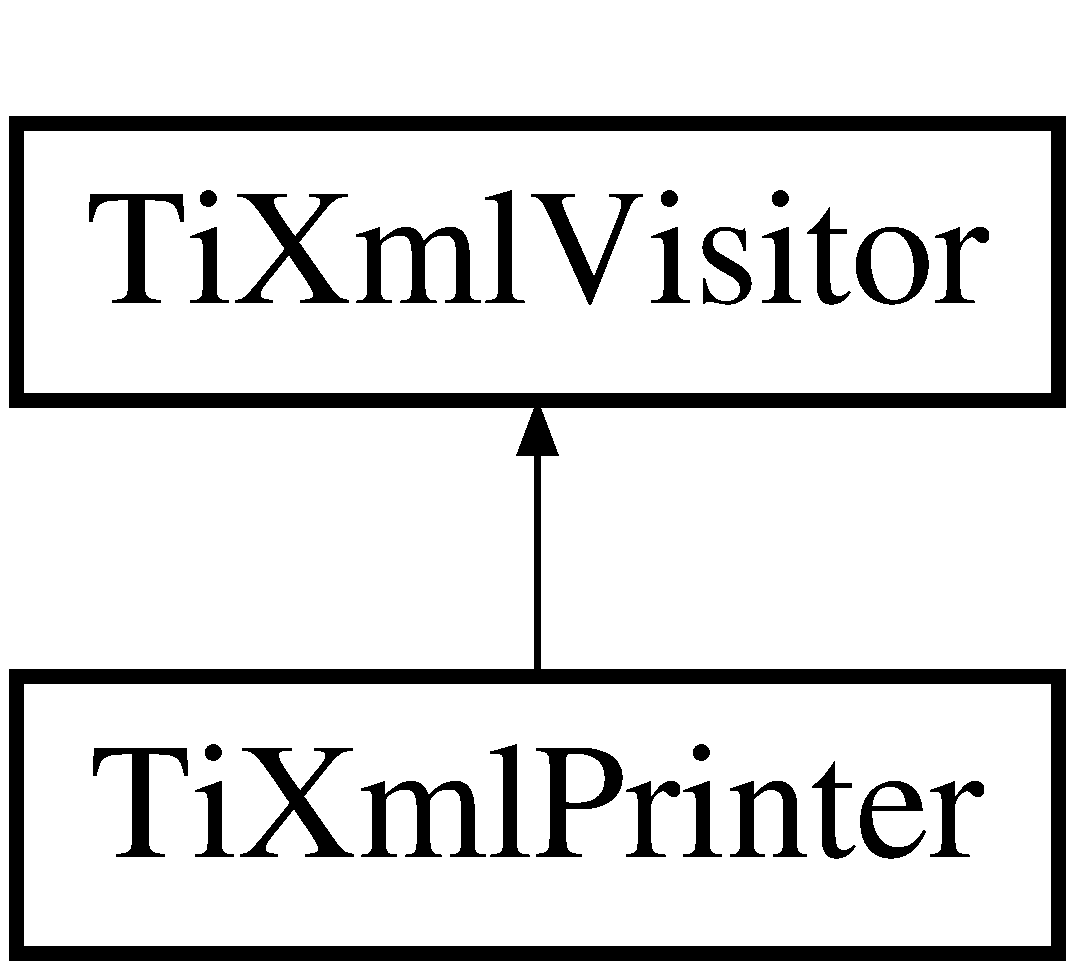
\includegraphics[height=2.000000cm]{class_ti_xml_printer}
\end{center}
\end{figure}
\subsection*{Public Member Functions}
\begin{DoxyCompactItemize}
\item 
\hypertarget{class_ti_xml_printer_a2ec73087db26ff4d2c4316c56f861db7}{
virtual bool \hyperlink{class_ti_xml_printer_a2ec73087db26ff4d2c4316c56f861db7}{VisitEnter} (const \hyperlink{class_ti_xml_document}{TiXmlDocument} \&doc)}
\label{class_ti_xml_printer_a2ec73087db26ff4d2c4316c56f861db7}

\begin{DoxyCompactList}\small\item\em Visit a document. \end{DoxyCompactList}\item 
\hypertarget{class_ti_xml_printer_a0a636046fa589b6d7f3e5bd025b3f33e}{
virtual bool \hyperlink{class_ti_xml_printer_a0a636046fa589b6d7f3e5bd025b3f33e}{VisitExit} (const \hyperlink{class_ti_xml_document}{TiXmlDocument} \&doc)}
\label{class_ti_xml_printer_a0a636046fa589b6d7f3e5bd025b3f33e}

\begin{DoxyCompactList}\small\item\em Visit a document. \end{DoxyCompactList}\item 
\hypertarget{class_ti_xml_printer_a6dccaf5ee4979f13877690afe28721e8}{
virtual bool \hyperlink{class_ti_xml_printer_a6dccaf5ee4979f13877690afe28721e8}{VisitEnter} (const \hyperlink{class_ti_xml_element}{TiXmlElement} \&element, const \hyperlink{class_ti_xml_attribute}{TiXmlAttribute} $\ast$firstAttribute)}
\label{class_ti_xml_printer_a6dccaf5ee4979f13877690afe28721e8}

\begin{DoxyCompactList}\small\item\em Visit an element. \end{DoxyCompactList}\item 
\hypertarget{class_ti_xml_printer_ae6a1df8271df4bf62d7873c38e34aa69}{
virtual bool \hyperlink{class_ti_xml_printer_ae6a1df8271df4bf62d7873c38e34aa69}{VisitExit} (const \hyperlink{class_ti_xml_element}{TiXmlElement} \&element)}
\label{class_ti_xml_printer_ae6a1df8271df4bf62d7873c38e34aa69}

\begin{DoxyCompactList}\small\item\em Visit an element. \end{DoxyCompactList}\item 
\hypertarget{class_ti_xml_printer_adaf7eec4dc43ad071ff52b60361574f5}{
virtual bool \hyperlink{class_ti_xml_printer_adaf7eec4dc43ad071ff52b60361574f5}{Visit} (const \hyperlink{class_ti_xml_declaration}{TiXmlDeclaration} \&declaration)}
\label{class_ti_xml_printer_adaf7eec4dc43ad071ff52b60361574f5}

\begin{DoxyCompactList}\small\item\em Visit a declaration. \end{DoxyCompactList}\item 
\hypertarget{class_ti_xml_printer_a0857c5d32c59b9a257f9a49cb9411df5}{
virtual bool \hyperlink{class_ti_xml_printer_a0857c5d32c59b9a257f9a49cb9411df5}{Visit} (const \hyperlink{class_ti_xml_text}{TiXmlText} \&text)}
\label{class_ti_xml_printer_a0857c5d32c59b9a257f9a49cb9411df5}

\begin{DoxyCompactList}\small\item\em Visit a text node. \end{DoxyCompactList}\item 
\hypertarget{class_ti_xml_printer_a9870423f5603630e6142f6bdb66dfb57}{
virtual bool \hyperlink{class_ti_xml_printer_a9870423f5603630e6142f6bdb66dfb57}{Visit} (const \hyperlink{class_ti_xml_comment}{TiXmlComment} \&comment)}
\label{class_ti_xml_printer_a9870423f5603630e6142f6bdb66dfb57}

\begin{DoxyCompactList}\small\item\em Visit a comment node. \end{DoxyCompactList}\item 
\hypertarget{class_ti_xml_printer_a08591a15c9a07afa83c24e08b03d6358}{
virtual bool \hyperlink{class_ti_xml_printer_a08591a15c9a07afa83c24e08b03d6358}{Visit} (const \hyperlink{class_ti_xml_unknown}{TiXmlUnknown} \&unknown)}
\label{class_ti_xml_printer_a08591a15c9a07afa83c24e08b03d6358}

\begin{DoxyCompactList}\small\item\em Visit an unknown node. \end{DoxyCompactList}\item 
void \hyperlink{class_ti_xml_printer_a213377a4070c7e625bae59716b089e5e}{SetIndent} (const char $\ast$\_\-indent)
\item 
\hypertarget{class_ti_xml_printer_abb33ec7d4bad6aaeb57f4304394b133d}{
const char $\ast$ \hyperlink{class_ti_xml_printer_abb33ec7d4bad6aaeb57f4304394b133d}{Indent} ()}
\label{class_ti_xml_printer_abb33ec7d4bad6aaeb57f4304394b133d}

\begin{DoxyCompactList}\small\item\em Query the indention string. \end{DoxyCompactList}\item 
void \hyperlink{class_ti_xml_printer_a4be1e37e69e3858c59635aa947174fe6}{SetLineBreak} (const char $\ast$\_\-lineBreak)
\item 
\hypertarget{class_ti_xml_printer_a11f1b4804a460b175ec244eb5724d96d}{
const char $\ast$ \hyperlink{class_ti_xml_printer_a11f1b4804a460b175ec244eb5724d96d}{LineBreak} ()}
\label{class_ti_xml_printer_a11f1b4804a460b175ec244eb5724d96d}

\begin{DoxyCompactList}\small\item\em Query the current line breaking string. \end{DoxyCompactList}\item 
void \hyperlink{class_ti_xml_printer_ab23a90629e374cb1cadca090468bbd19}{SetStreamPrinting} ()
\item 
\hypertarget{class_ti_xml_printer_a859eede9597d3e0355b77757be48735e}{
const char $\ast$ \hyperlink{class_ti_xml_printer_a859eede9597d3e0355b77757be48735e}{CStr} ()}
\label{class_ti_xml_printer_a859eede9597d3e0355b77757be48735e}

\begin{DoxyCompactList}\small\item\em Return the result. \end{DoxyCompactList}\item 
\hypertarget{class_ti_xml_printer_ad01375ae9199bd2f48252eaddce3039d}{
size\_\-t \hyperlink{class_ti_xml_printer_ad01375ae9199bd2f48252eaddce3039d}{Size} ()}
\label{class_ti_xml_printer_ad01375ae9199bd2f48252eaddce3039d}

\begin{DoxyCompactList}\small\item\em Return the length of the result string. \end{DoxyCompactList}\end{DoxyCompactItemize}


\subsection{Detailed Description}
Print to memory functionality. The \hyperlink{class_ti_xml_printer}{TiXmlPrinter} is useful when you need to:


\begin{DoxyEnumerate}
\item Print to memory (especially in non-\/STL mode)
\item Control formatting (line endings, etc.)
\end{DoxyEnumerate}

When constructed, the \hyperlink{class_ti_xml_printer}{TiXmlPrinter} is in its default \char`\"{}pretty printing\char`\"{} mode. Before calling Accept() you can call methods to control the printing of the XML document. After \hyperlink{class_ti_xml_node_acc0f88b7462c6cb73809d410a4f5bb86}{TiXmlNode::Accept()} is called, the printed document can be accessed via the \hyperlink{class_ti_xml_printer_a859eede9597d3e0355b77757be48735e}{CStr()}, Str(), and \hyperlink{class_ti_xml_printer_ad01375ae9199bd2f48252eaddce3039d}{Size()} methods.

\hyperlink{class_ti_xml_printer}{TiXmlPrinter} uses the Visitor API. \begin{DoxyVerb}
	TiXmlPrinter printer;
	printer.SetIndent( "\t" );

	doc.Accept( &printer );
	fprintf( stdout, "%s", printer.CStr() );
	\end{DoxyVerb}
 

\subsection{Member Function Documentation}
\hypertarget{class_ti_xml_printer_a213377a4070c7e625bae59716b089e5e}{
\index{TiXmlPrinter@{TiXmlPrinter}!SetIndent@{SetIndent}}
\index{SetIndent@{SetIndent}!TiXmlPrinter@{TiXmlPrinter}}
\subsubsection[{SetIndent}]{\setlength{\rightskip}{0pt plus 5cm}void TiXmlPrinter::SetIndent (
\begin{DoxyParamCaption}
\item[{const char $\ast$}]{\_\-indent}
\end{DoxyParamCaption}
)\hspace{0.3cm}{\ttfamily  \mbox{[}inline\mbox{]}}}}
\label{class_ti_xml_printer_a213377a4070c7e625bae59716b089e5e}
Set the indent characters for printing. By default 4 spaces but tab () is also useful, or null/empty string for no indentation. \hypertarget{class_ti_xml_printer_a4be1e37e69e3858c59635aa947174fe6}{
\index{TiXmlPrinter@{TiXmlPrinter}!SetLineBreak@{SetLineBreak}}
\index{SetLineBreak@{SetLineBreak}!TiXmlPrinter@{TiXmlPrinter}}
\subsubsection[{SetLineBreak}]{\setlength{\rightskip}{0pt plus 5cm}void TiXmlPrinter::SetLineBreak (
\begin{DoxyParamCaption}
\item[{const char $\ast$}]{\_\-lineBreak}
\end{DoxyParamCaption}
)\hspace{0.3cm}{\ttfamily  \mbox{[}inline\mbox{]}}}}
\label{class_ti_xml_printer_a4be1e37e69e3858c59635aa947174fe6}
Set the line breaking string. By default set to newline (\par
). Some operating systems prefer other characters, or can be set to the null/empty string for no indenation. \hypertarget{class_ti_xml_printer_ab23a90629e374cb1cadca090468bbd19}{
\index{TiXmlPrinter@{TiXmlPrinter}!SetStreamPrinting@{SetStreamPrinting}}
\index{SetStreamPrinting@{SetStreamPrinting}!TiXmlPrinter@{TiXmlPrinter}}
\subsubsection[{SetStreamPrinting}]{\setlength{\rightskip}{0pt plus 5cm}void TiXmlPrinter::SetStreamPrinting (
\begin{DoxyParamCaption}
{}
\end{DoxyParamCaption}
)\hspace{0.3cm}{\ttfamily  \mbox{[}inline\mbox{]}}}}
\label{class_ti_xml_printer_ab23a90629e374cb1cadca090468bbd19}
Switch over to \char`\"{}stream printing\char`\"{} which is the most dense formatting without linebreaks. Common when the XML is needed for network transmission. 

The documentation for this class was generated from the following files:\begin{DoxyCompactItemize}
\item 
/home/cshome/m/mabrams/345/txtEngine/tinyxml.h\item 
/home/cshome/m/mabrams/345/txtEngine/tinyxml.cpp\end{DoxyCompactItemize}

\hypertarget{class_ti_xml_string}{
\section{\-Ti\-Xml\-String \-Class \-Reference}
\label{class_ti_xml_string}\index{\-Ti\-Xml\-String@{\-Ti\-Xml\-String}}
}


\-Inheritance diagram for \-Ti\-Xml\-String\-:
\subsection*{\-Classes}
\begin{DoxyCompactItemize}
\item 
struct {\bfseries \-Rep}
\end{DoxyCompactItemize}
\subsection*{\-Public \-Types}
\begin{DoxyCompactItemize}
\item 
\hypertarget{class_ti_xml_string_abeb2c1893a04c17904f7c06546d0b971}{
typedef size\-\_\-t {\bfseries size\-\_\-type}}
\label{class_ti_xml_string_abeb2c1893a04c17904f7c06546d0b971}

\end{DoxyCompactItemize}
\subsection*{\-Public \-Member \-Functions}
\begin{DoxyCompactItemize}
\item 
\hypertarget{class_ti_xml_string_ac80fe17693a438c9ab2591664743fcb6}{
{\bfseries \-Ti\-Xml\-String} (const \hyperlink{class_ti_xml_string}{\-Ti\-Xml\-String} \&copy)}
\label{class_ti_xml_string_ac80fe17693a438c9ab2591664743fcb6}

\item 
\hypertarget{class_ti_xml_string_aa3b32bd2891a757c9f36c21db44c81d2}{
\-T\-I\-X\-M\-L\-\_\-\-E\-X\-P\-L\-I\-C\-I\-T {\bfseries \-Ti\-Xml\-String} (const char $\ast$copy)}
\label{class_ti_xml_string_aa3b32bd2891a757c9f36c21db44c81d2}

\item 
\hypertarget{class_ti_xml_string_a4b17ea5c5db986f14827223dfa8f1547}{
\-T\-I\-X\-M\-L\-\_\-\-E\-X\-P\-L\-I\-C\-I\-T {\bfseries \-Ti\-Xml\-String} (const char $\ast$str, size\-\_\-type len)}
\label{class_ti_xml_string_a4b17ea5c5db986f14827223dfa8f1547}

\item 
\hypertarget{class_ti_xml_string_ae0bc6147afc0ec2aa0da3a3c0a8fcfb0}{
\hyperlink{class_ti_xml_string}{\-Ti\-Xml\-String} \& {\bfseries operator=} (const char $\ast$copy)}
\label{class_ti_xml_string_ae0bc6147afc0ec2aa0da3a3c0a8fcfb0}

\item 
\hypertarget{class_ti_xml_string_ab1f1f5d3eceaa0f22d0a7e6055ea81b0}{
\hyperlink{class_ti_xml_string}{\-Ti\-Xml\-String} \& {\bfseries operator=} (const \hyperlink{class_ti_xml_string}{\-Ti\-Xml\-String} \&copy)}
\label{class_ti_xml_string_ab1f1f5d3eceaa0f22d0a7e6055ea81b0}

\item 
\hypertarget{class_ti_xml_string_ab56336ac2aa2a08d24a71eb9a2b502a5}{
\hyperlink{class_ti_xml_string}{\-Ti\-Xml\-String} \& {\bfseries operator+=} (const char $\ast$suffix)}
\label{class_ti_xml_string_ab56336ac2aa2a08d24a71eb9a2b502a5}

\item 
\hypertarget{class_ti_xml_string_a6aa09d5240470b76d54ec709e04f8c13}{
\hyperlink{class_ti_xml_string}{\-Ti\-Xml\-String} \& {\bfseries operator+=} (char single)}
\label{class_ti_xml_string_a6aa09d5240470b76d54ec709e04f8c13}

\item 
\hypertarget{class_ti_xml_string_afdcae5ea2b4d9e194dc21226b817f417}{
\hyperlink{class_ti_xml_string}{\-Ti\-Xml\-String} \& {\bfseries operator+=} (const \hyperlink{class_ti_xml_string}{\-Ti\-Xml\-String} \&suffix)}
\label{class_ti_xml_string_afdcae5ea2b4d9e194dc21226b817f417}

\item 
\hypertarget{class_ti_xml_string_a5581ca641d915551d3cda90f8e7bf49b}{
const char $\ast$ {\bfseries c\-\_\-str} () const }
\label{class_ti_xml_string_a5581ca641d915551d3cda90f8e7bf49b}

\item 
\hypertarget{class_ti_xml_string_a00abc60f135c7ca1951c7334cc2c7993}{
const char $\ast$ {\bfseries data} () const }
\label{class_ti_xml_string_a00abc60f135c7ca1951c7334cc2c7993}

\item 
\hypertarget{class_ti_xml_string_a3202f27d139a3fac79205f1f3c707727}{
size\-\_\-type {\bfseries length} () const }
\label{class_ti_xml_string_a3202f27d139a3fac79205f1f3c707727}

\item 
\hypertarget{class_ti_xml_string_a96103e5c0f67e987fa48527e1f47a1f6}{
size\-\_\-type {\bfseries size} () const }
\label{class_ti_xml_string_a96103e5c0f67e987fa48527e1f47a1f6}

\item 
\hypertarget{class_ti_xml_string_a9a61e1d11cdb71bea4a4ed79caa793f4}{
bool {\bfseries empty} () const }
\label{class_ti_xml_string_a9a61e1d11cdb71bea4a4ed79caa793f4}

\item 
\hypertarget{class_ti_xml_string_a76e4d6aba7845f4cf9c02332a5fbf916}{
size\-\_\-type {\bfseries capacity} () const }
\label{class_ti_xml_string_a76e4d6aba7845f4cf9c02332a5fbf916}

\item 
\hypertarget{class_ti_xml_string_a6763093267bbdecbf03f8840bc349877}{
const char \& {\bfseries at} (size\-\_\-type index) const }
\label{class_ti_xml_string_a6763093267bbdecbf03f8840bc349877}

\item 
\hypertarget{class_ti_xml_string_ae8cdc1d46c538536b786f7ae03c0c1d9}{
char \& {\bfseries operator\mbox{[}$\,$\mbox{]}} (size\-\_\-type index) const }
\label{class_ti_xml_string_ae8cdc1d46c538536b786f7ae03c0c1d9}

\item 
\hypertarget{class_ti_xml_string_a5c2b368b5eafe075fd9565cbcbd4c2f9}{
size\-\_\-type {\bfseries find} (char lookup) const }
\label{class_ti_xml_string_a5c2b368b5eafe075fd9565cbcbd4c2f9}

\item 
\hypertarget{class_ti_xml_string_a5f2a6fd565751410b392f249a9786db4}{
size\-\_\-type {\bfseries find} (char tofind, size\-\_\-type offset) const }
\label{class_ti_xml_string_a5f2a6fd565751410b392f249a9786db4}

\item 
\hypertarget{class_ti_xml_string_ab20e06e4c666abf3bdbfb3a1191d4888}{
void {\bfseries clear} ()}
\label{class_ti_xml_string_ab20e06e4c666abf3bdbfb3a1191d4888}

\item 
\hypertarget{class_ti_xml_string_a88ecf9f0f00cb5c67b6b637958d7049c}{
void {\bfseries reserve} (size\-\_\-type cap)}
\label{class_ti_xml_string_a88ecf9f0f00cb5c67b6b637958d7049c}

\item 
\hypertarget{class_ti_xml_string_ac72f3d9149b7812c1e6c59402014d0d5}{
\hyperlink{class_ti_xml_string}{\-Ti\-Xml\-String} \& {\bfseries assign} (const char $\ast$str, size\-\_\-type len)}
\label{class_ti_xml_string_ac72f3d9149b7812c1e6c59402014d0d5}

\item 
\hypertarget{class_ti_xml_string_ad44b21700d2ec24a511367b222b643fb}{
\hyperlink{class_ti_xml_string}{\-Ti\-Xml\-String} \& {\bfseries append} (const char $\ast$str, size\-\_\-type len)}
\label{class_ti_xml_string_ad44b21700d2ec24a511367b222b643fb}

\item 
\hypertarget{class_ti_xml_string_aa392cbc180752a79f007f4f9280c7762}{
void {\bfseries swap} (\hyperlink{class_ti_xml_string}{\-Ti\-Xml\-String} \&other)}
\label{class_ti_xml_string_aa392cbc180752a79f007f4f9280c7762}

\end{DoxyCompactItemize}
\subsection*{\-Static \-Public \-Attributes}
\begin{DoxyCompactItemize}
\item 
\hypertarget{class_ti_xml_string_a8f4422d227088dc7bec96f479b275d0a}{
static const size\-\_\-type {\bfseries npos} = static\-\_\-cast$<$ \-Ti\-Xml\-String\-::size\-\_\-type $>$(-\/1)}
\label{class_ti_xml_string_a8f4422d227088dc7bec96f479b275d0a}

\end{DoxyCompactItemize}


\-The documentation for this class was generated from the following files\-:\begin{DoxyCompactItemize}
\item 
/home/cshome/m/mabrams/345/txt\-Engine/tinystr.\-h\item 
/home/cshome/m/mabrams/345/txt\-Engine/tinystr.\-cpp\end{DoxyCompactItemize}

\hypertarget{class_ti_xml_text}{
\section{\-Ti\-Xml\-Text \-Class \-Reference}
\label{class_ti_xml_text}\index{\-Ti\-Xml\-Text@{\-Ti\-Xml\-Text}}
}


{\ttfamily \#include $<$tinyxml.\-h$>$}



\-Inheritance diagram for \-Ti\-Xml\-Text\-:


\-Collaboration diagram for \-Ti\-Xml\-Text\-:
\subsection*{\-Public \-Member \-Functions}
\begin{DoxyCompactItemize}
\item 
\hyperlink{class_ti_xml_text_af659e77c6b87d684827f35a8f4895960}{\-Ti\-Xml\-Text} (const char $\ast$init\-Value)
\item 
\hypertarget{class_ti_xml_text_a8d2cc1b4af2208cbb0171cf20f6815d1}{
{\bfseries \-Ti\-Xml\-Text} (const \hyperlink{class_ti_xml_text}{\-Ti\-Xml\-Text} \&copy)}
\label{class_ti_xml_text_a8d2cc1b4af2208cbb0171cf20f6815d1}

\item 
\hypertarget{class_ti_xml_text_aed5b13f9c1b804c616fd533882c29f57}{
\hyperlink{class_ti_xml_text}{\-Ti\-Xml\-Text} \& {\bfseries operator=} (const \hyperlink{class_ti_xml_text}{\-Ti\-Xml\-Text} \&base)}
\label{class_ti_xml_text_aed5b13f9c1b804c616fd533882c29f57}

\item 
virtual void \hyperlink{class_ti_xml_text_ae74d56c5b3ddec6cc3103dd51821af92}{\-Print} (\-F\-I\-L\-E $\ast$cfile, int depth) const 
\item 
\hypertarget{class_ti_xml_text_ad1a6a6b83fa2271022dd97c072a2b586}{
bool \hyperlink{class_ti_xml_text_ad1a6a6b83fa2271022dd97c072a2b586}{\-C\-D\-A\-T\-A} () const }
\label{class_ti_xml_text_ad1a6a6b83fa2271022dd97c072a2b586}

\begin{DoxyCompactList}\small\item\em \-Queries whether this represents text using a \-C\-D\-A\-T\-A section. \end{DoxyCompactList}\item 
\hypertarget{class_ti_xml_text_acb17ff7c5d09b2c839393445a3de5ea9}{
void \hyperlink{class_ti_xml_text_acb17ff7c5d09b2c839393445a3de5ea9}{\-Set\-C\-D\-A\-T\-A} (bool \-\_\-cdata)}
\label{class_ti_xml_text_acb17ff7c5d09b2c839393445a3de5ea9}

\begin{DoxyCompactList}\small\item\em \-Turns on or off a \-C\-D\-A\-T\-A representation of text. \end{DoxyCompactList}\item 
\hypertarget{class_ti_xml_text_a8d2dcfa41fc73d3e62dacc2fcf633819}{
virtual const char $\ast$ {\bfseries \-Parse} (const char $\ast$p, \hyperlink{class_ti_xml_parsing_data}{\-Ti\-Xml\-Parsing\-Data} $\ast$data, \-Ti\-Xml\-Encoding encoding)}
\label{class_ti_xml_text_a8d2dcfa41fc73d3e62dacc2fcf633819}

\item 
virtual const \hyperlink{class_ti_xml_text}{\-Ti\-Xml\-Text} $\ast$ \hyperlink{class_ti_xml_text_a895bf34ffad17f7439ab2a52b9651648}{\-To\-Text} () const 
\item 
virtual \hyperlink{class_ti_xml_text}{\-Ti\-Xml\-Text} $\ast$ \hyperlink{class_ti_xml_text_ae7c3a8fd3e4dbf6c0c4363a943d72f5b}{\-To\-Text} ()
\item 
virtual bool \hyperlink{class_ti_xml_text_a43b9954ebf679557fac1a4453f337b7c}{\-Accept} (\hyperlink{class_ti_xml_visitor}{\-Ti\-Xml\-Visitor} $\ast$content) const 
\end{DoxyCompactItemize}
\subsection*{\-Protected \-Member \-Functions}
\begin{DoxyCompactItemize}
\item 
\hypertarget{class_ti_xml_text_adde1869dfb029be50713fbfd8ce4d21f}{
virtual \hyperlink{class_ti_xml_node}{\-Ti\-Xml\-Node} $\ast$ \hyperlink{class_ti_xml_text_adde1869dfb029be50713fbfd8ce4d21f}{\-Clone} () const }
\label{class_ti_xml_text_adde1869dfb029be50713fbfd8ce4d21f}

\begin{DoxyCompactList}\small\item\em \mbox{[}internal use\mbox{]} \-Creates a new \-Element and returns it. \end{DoxyCompactList}\item 
\hypertarget{class_ti_xml_text_adcec7d9b6fccfc5777452bb97e6031c1}{
void {\bfseries \-Copy\-To} (\hyperlink{class_ti_xml_text}{\-Ti\-Xml\-Text} $\ast$target) const }
\label{class_ti_xml_text_adcec7d9b6fccfc5777452bb97e6031c1}

\item 
\hypertarget{class_ti_xml_text_a1c120428e3b3cf24d79706e6d2b65aa6}{
bool {\bfseries \-Blank} () const }
\label{class_ti_xml_text_a1c120428e3b3cf24d79706e6d2b65aa6}

\end{DoxyCompactItemize}
\subsection*{\-Friends}
\begin{DoxyCompactItemize}
\item 
\hypertarget{class_ti_xml_text_ab6592e32cb9132be517cc12a70564c4b}{
class {\bfseries \-Ti\-Xml\-Element}}
\label{class_ti_xml_text_ab6592e32cb9132be517cc12a70564c4b}

\end{DoxyCompactItemize}


\subsection{\-Detailed \-Description}
\-X\-M\-L text. \-A text node can have 2 ways to output the next. \char`\"{}normal\char`\"{} output and \-C\-D\-A\-T\-A. \-It will default to the mode it was parsed from the \-X\-M\-L file and you generally want to leave it alone, but you can change the output mode with \hyperlink{class_ti_xml_text_acb17ff7c5d09b2c839393445a3de5ea9}{\-Set\-C\-D\-A\-T\-A()} and query it with \hyperlink{class_ti_xml_text_ad1a6a6b83fa2271022dd97c072a2b586}{\-C\-D\-A\-T\-A()}. 

\subsection{\-Constructor \& \-Destructor \-Documentation}
\hypertarget{class_ti_xml_text_af659e77c6b87d684827f35a8f4895960}{
\index{\-Ti\-Xml\-Text@{\-Ti\-Xml\-Text}!\-Ti\-Xml\-Text@{\-Ti\-Xml\-Text}}
\index{\-Ti\-Xml\-Text@{\-Ti\-Xml\-Text}!TiXmlText@{\-Ti\-Xml\-Text}}
\subsubsection[{\-Ti\-Xml\-Text}]{\setlength{\rightskip}{0pt plus 5cm}\-Ti\-Xml\-Text\-::\-Ti\-Xml\-Text (
\begin{DoxyParamCaption}
\item[{const char $\ast$}]{init\-Value}
\end{DoxyParamCaption}
)\hspace{0.3cm}{\ttfamily  \mbox{[}inline\mbox{]}}}}
\label{class_ti_xml_text_af659e77c6b87d684827f35a8f4895960}
\-Constructor for text element. \-By default, it is treated as normal, encoded text. \-If you want it be output as a \-C\-D\-A\-T\-A text element, set the parameter \-\_\-cdata to 'true' 

\-Here is the call graph for this function\-:




\-Here is the caller graph for this function\-:




\subsection{\-Member \-Function \-Documentation}
\hypertarget{class_ti_xml_text_a43b9954ebf679557fac1a4453f337b7c}{
\index{\-Ti\-Xml\-Text@{\-Ti\-Xml\-Text}!\-Accept@{\-Accept}}
\index{\-Accept@{\-Accept}!TiXmlText@{\-Ti\-Xml\-Text}}
\subsubsection[{\-Accept}]{\setlength{\rightskip}{0pt plus 5cm}bool \-Ti\-Xml\-Text\-::\-Accept (
\begin{DoxyParamCaption}
\item[{{\bf \-Ti\-Xml\-Visitor} $\ast$}]{content}
\end{DoxyParamCaption}
) const\hspace{0.3cm}{\ttfamily  \mbox{[}virtual\mbox{]}}}}
\label{class_ti_xml_text_a43b9954ebf679557fac1a4453f337b7c}
\-Walk the \-X\-M\-L tree visiting this node and all of its children. 

\-Implements \hyperlink{class_ti_xml_node_acc0f88b7462c6cb73809d410a4f5bb86}{\-Ti\-Xml\-Node}.



\-Here is the call graph for this function\-:


\hypertarget{class_ti_xml_text_ae74d56c5b3ddec6cc3103dd51821af92}{
\index{\-Ti\-Xml\-Text@{\-Ti\-Xml\-Text}!\-Print@{\-Print}}
\index{\-Print@{\-Print}!TiXmlText@{\-Ti\-Xml\-Text}}
\subsubsection[{\-Print}]{\setlength{\rightskip}{0pt plus 5cm}void \-Ti\-Xml\-Text\-::\-Print (
\begin{DoxyParamCaption}
\item[{\-F\-I\-L\-E $\ast$}]{cfile, }
\item[{int}]{depth}
\end{DoxyParamCaption}
) const\hspace{0.3cm}{\ttfamily  \mbox{[}virtual\mbox{]}}}}
\label{class_ti_xml_text_ae74d56c5b3ddec6cc3103dd51821af92}
\-All \-Tiny\-Xml classes can print themselves to a filestream or the string class (\hyperlink{class_ti_xml_string}{\-Ti\-Xml\-String} in non-\/\-S\-T\-L mode, std\-::string in \-S\-T\-L mode.) \-Either or both cfile and str can be null.

\-This is a formatted print, and will insert tabs and newlines.

(\-For an unformatted stream, use the $<$$<$ operator.) 

\-Implements \hyperlink{class_ti_xml_base_a0de56b3f2ef14c65091a3b916437b512}{\-Ti\-Xml\-Base}.



\-Here is the call graph for this function\-:


\hypertarget{class_ti_xml_text_a895bf34ffad17f7439ab2a52b9651648}{
\index{\-Ti\-Xml\-Text@{\-Ti\-Xml\-Text}!\-To\-Text@{\-To\-Text}}
\index{\-To\-Text@{\-To\-Text}!TiXmlText@{\-Ti\-Xml\-Text}}
\subsubsection[{\-To\-Text}]{\setlength{\rightskip}{0pt plus 5cm}virtual const {\bf \-Ti\-Xml\-Text}$\ast$ \-Ti\-Xml\-Text\-::\-To\-Text (
\begin{DoxyParamCaption}
{}
\end{DoxyParamCaption}
) const\hspace{0.3cm}{\ttfamily  \mbox{[}inline, virtual\mbox{]}}}}
\label{class_ti_xml_text_a895bf34ffad17f7439ab2a52b9651648}
$<$ \-Cast to a more defined type. \-Will return null not of the requested type. 

\-Reimplemented from \hyperlink{class_ti_xml_node_a95a46a52c525992d6b4ee08beb14cd69}{\-Ti\-Xml\-Node}.

\hypertarget{class_ti_xml_text_ae7c3a8fd3e4dbf6c0c4363a943d72f5b}{
\index{\-Ti\-Xml\-Text@{\-Ti\-Xml\-Text}!\-To\-Text@{\-To\-Text}}
\index{\-To\-Text@{\-To\-Text}!TiXmlText@{\-Ti\-Xml\-Text}}
\subsubsection[{\-To\-Text}]{\setlength{\rightskip}{0pt plus 5cm}virtual {\bf \-Ti\-Xml\-Text}$\ast$ \-Ti\-Xml\-Text\-::\-To\-Text (
\begin{DoxyParamCaption}
{}
\end{DoxyParamCaption}
)\hspace{0.3cm}{\ttfamily  \mbox{[}inline, virtual\mbox{]}}}}
\label{class_ti_xml_text_ae7c3a8fd3e4dbf6c0c4363a943d72f5b}
$<$ \-Cast to a more defined type. \-Will return null not of the requested type. 

\-Reimplemented from \hyperlink{class_ti_xml_node_a3ddfbcac78fbea041fad57e5c6d60a03}{\-Ti\-Xml\-Node}.



\-The documentation for this class was generated from the following files\-:\begin{DoxyCompactItemize}
\item 
/home/cshome/m/mabrams/345/txt\-Engine/tinyxml.\-h\item 
/home/cshome/m/mabrams/345/txt\-Engine/tinyxml.\-cpp\item 
/home/cshome/m/mabrams/345/txt\-Engine/tinyxmlparser.\-cpp\end{DoxyCompactItemize}

\hypertarget{class_ti_xml_unknown}{
\section{TiXmlUnknown Class Reference}
\label{class_ti_xml_unknown}\index{TiXmlUnknown@{TiXmlUnknown}}
}


{\ttfamily \#include $<$tinyxml.h$>$}

Inheritance diagram for TiXmlUnknown:\begin{figure}[H]
\begin{center}
\leavevmode
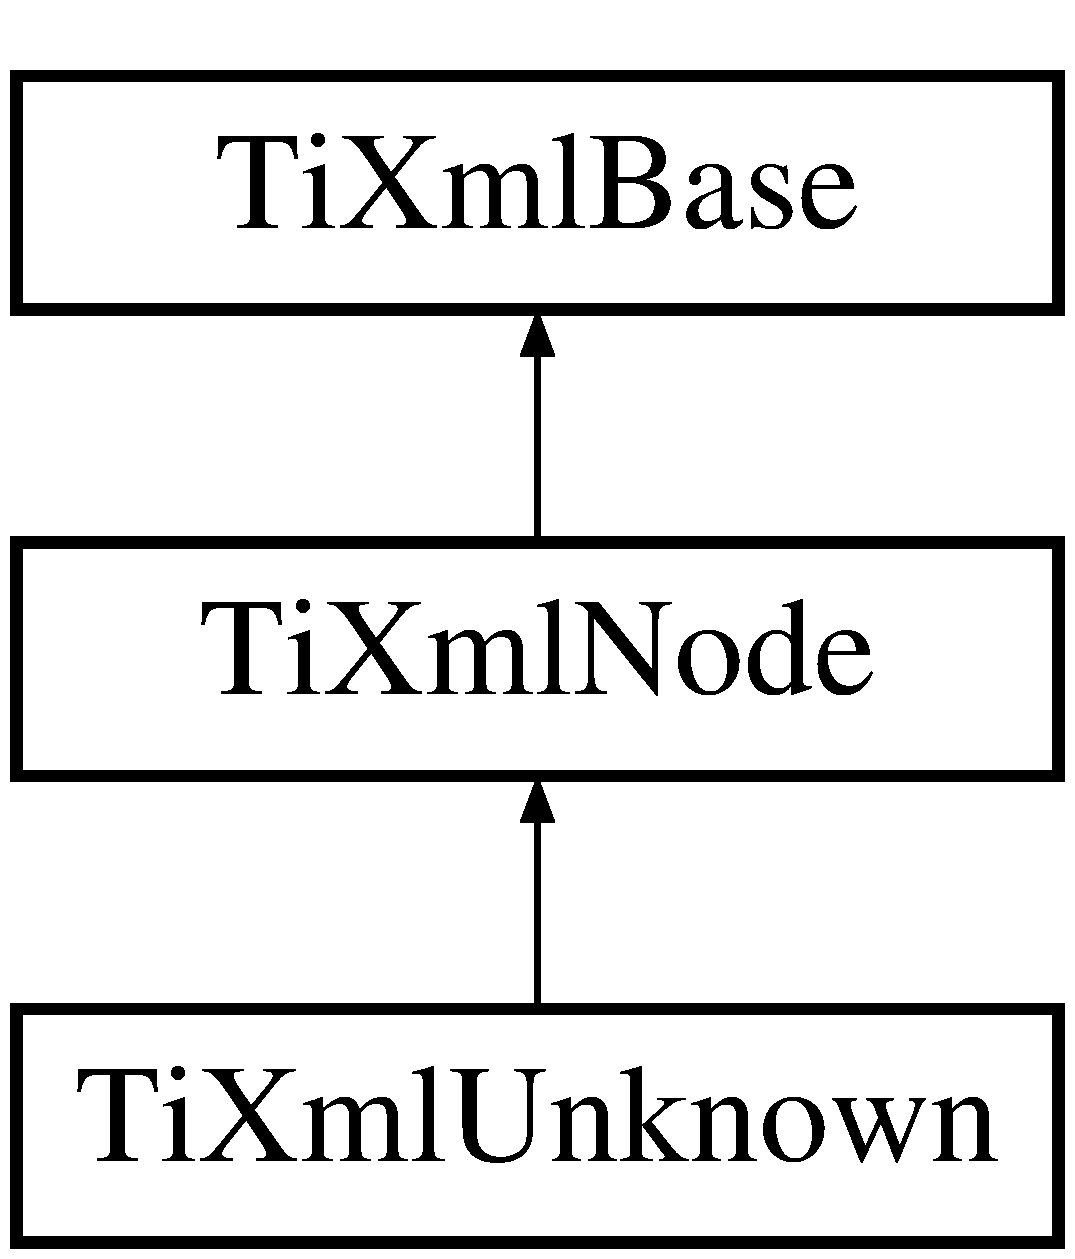
\includegraphics[height=3.000000cm]{class_ti_xml_unknown}
\end{center}
\end{figure}
\subsection*{Public Member Functions}
\begin{DoxyCompactItemize}
\item 
\hypertarget{class_ti_xml_unknown_abe798ff4feea31474850c7f0de6bdf5e}{
{\bfseries TiXmlUnknown} (const \hyperlink{class_ti_xml_unknown}{TiXmlUnknown} \&copy)}
\label{class_ti_xml_unknown_abe798ff4feea31474850c7f0de6bdf5e}

\item 
\hypertarget{class_ti_xml_unknown_a60560b5aacb4bdc8b2b5f02f0a99c5c0}{
\hyperlink{class_ti_xml_unknown}{TiXmlUnknown} \& {\bfseries operator=} (const \hyperlink{class_ti_xml_unknown}{TiXmlUnknown} \&copy)}
\label{class_ti_xml_unknown_a60560b5aacb4bdc8b2b5f02f0a99c5c0}

\item 
\hypertarget{class_ti_xml_unknown_a675c4b2684af35e4c7649b7fd5ae598d}{
virtual \hyperlink{class_ti_xml_node}{TiXmlNode} $\ast$ \hyperlink{class_ti_xml_unknown_a675c4b2684af35e4c7649b7fd5ae598d}{Clone} () const }
\label{class_ti_xml_unknown_a675c4b2684af35e4c7649b7fd5ae598d}

\begin{DoxyCompactList}\small\item\em Creates a copy of this Unknown and returns it. \end{DoxyCompactList}\item 
virtual void \hyperlink{class_ti_xml_unknown_a025f19c21ef01ea9be50febb8fe0ba06}{Print} (FILE $\ast$cfile, int depth) const 
\item 
\hypertarget{class_ti_xml_unknown_aa51c2694e4177b5f0b5429ee5a81b58d}{
virtual const char $\ast$ {\bfseries Parse} (const char $\ast$p, \hyperlink{class_ti_xml_parsing_data}{TiXmlParsingData} $\ast$data, TiXmlEncoding encoding)}
\label{class_ti_xml_unknown_aa51c2694e4177b5f0b5429ee5a81b58d}

\item 
\hypertarget{class_ti_xml_unknown_ab0313e5fe77987d746ac1a97a254419d}{
virtual const \hyperlink{class_ti_xml_unknown}{TiXmlUnknown} $\ast$ \hyperlink{class_ti_xml_unknown_ab0313e5fe77987d746ac1a97a254419d}{ToUnknown} () const }
\label{class_ti_xml_unknown_ab0313e5fe77987d746ac1a97a254419d}

\begin{DoxyCompactList}\small\item\em Cast to a more defined type. Will return null not of the requested type. \end{DoxyCompactList}\item 
\hypertarget{class_ti_xml_unknown_a67c9fd22940e8c47f706a72cdd2e332c}{
virtual \hyperlink{class_ti_xml_unknown}{TiXmlUnknown} $\ast$ \hyperlink{class_ti_xml_unknown_a67c9fd22940e8c47f706a72cdd2e332c}{ToUnknown} ()}
\label{class_ti_xml_unknown_a67c9fd22940e8c47f706a72cdd2e332c}

\begin{DoxyCompactList}\small\item\em Cast to a more defined type. Will return null not of the requested type. \end{DoxyCompactList}\item 
virtual bool \hyperlink{class_ti_xml_unknown_a4e54d7482e05a837cf83c925cc683380}{Accept} (\hyperlink{class_ti_xml_visitor}{TiXmlVisitor} $\ast$content) const 
\end{DoxyCompactItemize}
\subsection*{Protected Member Functions}
\begin{DoxyCompactItemize}
\item 
\hypertarget{class_ti_xml_unknown_a08ca7b225a2bcb604d3c72e199d33408}{
void {\bfseries CopyTo} (\hyperlink{class_ti_xml_unknown}{TiXmlUnknown} $\ast$target) const }
\label{class_ti_xml_unknown_a08ca7b225a2bcb604d3c72e199d33408}

\end{DoxyCompactItemize}


\subsection{Detailed Description}
Any tag that tinyXml doesn't recognize is saved as an unknown. It is a tag of text, but should not be modified. It will be written back to the XML, unchanged, when the file is saved.

DTD tags get thrown into TiXmlUnknowns. 

\subsection{Member Function Documentation}
\hypertarget{class_ti_xml_unknown_a4e54d7482e05a837cf83c925cc683380}{
\index{TiXmlUnknown@{TiXmlUnknown}!Accept@{Accept}}
\index{Accept@{Accept}!TiXmlUnknown@{TiXmlUnknown}}
\subsubsection[{Accept}]{\setlength{\rightskip}{0pt plus 5cm}bool TiXmlUnknown::Accept (
\begin{DoxyParamCaption}
\item[{{\bf TiXmlVisitor} $\ast$}]{content}
\end{DoxyParamCaption}
) const\hspace{0.3cm}{\ttfamily  \mbox{[}virtual\mbox{]}}}}
\label{class_ti_xml_unknown_a4e54d7482e05a837cf83c925cc683380}
Walk the XML tree visiting this node and all of its children. 

Implements \hyperlink{class_ti_xml_node_acc0f88b7462c6cb73809d410a4f5bb86}{TiXmlNode}.

\hypertarget{class_ti_xml_unknown_a025f19c21ef01ea9be50febb8fe0ba06}{
\index{TiXmlUnknown@{TiXmlUnknown}!Print@{Print}}
\index{Print@{Print}!TiXmlUnknown@{TiXmlUnknown}}
\subsubsection[{Print}]{\setlength{\rightskip}{0pt plus 5cm}void TiXmlUnknown::Print (
\begin{DoxyParamCaption}
\item[{FILE $\ast$}]{cfile, }
\item[{int}]{depth}
\end{DoxyParamCaption}
) const\hspace{0.3cm}{\ttfamily  \mbox{[}virtual\mbox{]}}}}
\label{class_ti_xml_unknown_a025f19c21ef01ea9be50febb8fe0ba06}
All TinyXml classes can print themselves to a filestream or the string class (\hyperlink{class_ti_xml_string}{TiXmlString} in non-\/STL mode, std::string in STL mode.) Either or both cfile and str can be null.

This is a formatted print, and will insert tabs and newlines.

(For an unformatted stream, use the $<$$<$ operator.) 

Implements \hyperlink{class_ti_xml_base_a0de56b3f2ef14c65091a3b916437b512}{TiXmlBase}.



The documentation for this class was generated from the following files:\begin{DoxyCompactItemize}
\item 
/home/cshome/m/mabrams/345/txtEngine/tinyxml.h\item 
/home/cshome/m/mabrams/345/txtEngine/tinyxml.cpp\item 
/home/cshome/m/mabrams/345/txtEngine/tinyxmlparser.cpp\end{DoxyCompactItemize}

\hypertarget{class_ti_xml_visitor}{
\section{\-Ti\-Xml\-Visitor \-Class \-Reference}
\label{class_ti_xml_visitor}\index{\-Ti\-Xml\-Visitor@{\-Ti\-Xml\-Visitor}}
}


{\ttfamily \#include $<$tinyxml.\-h$>$}



\-Inheritance diagram for \-Ti\-Xml\-Visitor\-:
\subsection*{\-Public \-Member \-Functions}
\begin{DoxyCompactItemize}
\item 
\hypertarget{class_ti_xml_visitor_a07baecb52dd7d8716ae2a48ad0956ee0}{
virtual bool \hyperlink{class_ti_xml_visitor_a07baecb52dd7d8716ae2a48ad0956ee0}{\-Visit\-Enter} (const \hyperlink{class_ti_xml_document}{\-Ti\-Xml\-Document} \&)}
\label{class_ti_xml_visitor_a07baecb52dd7d8716ae2a48ad0956ee0}

\begin{DoxyCompactList}\small\item\em \-Visit a document. \end{DoxyCompactList}\item 
\hypertarget{class_ti_xml_visitor_aa0ade4f27087447e93974e975c3246ad}{
virtual bool \hyperlink{class_ti_xml_visitor_aa0ade4f27087447e93974e975c3246ad}{\-Visit\-Exit} (const \hyperlink{class_ti_xml_document}{\-Ti\-Xml\-Document} \&)}
\label{class_ti_xml_visitor_aa0ade4f27087447e93974e975c3246ad}

\begin{DoxyCompactList}\small\item\em \-Visit a document. \end{DoxyCompactList}\item 
\hypertarget{class_ti_xml_visitor_af6c6178ffa517bbdba95d70490875fff}{
virtual bool \hyperlink{class_ti_xml_visitor_af6c6178ffa517bbdba95d70490875fff}{\-Visit\-Enter} (const \hyperlink{class_ti_xml_element}{\-Ti\-Xml\-Element} \&, const \hyperlink{class_ti_xml_attribute}{\-Ti\-Xml\-Attribute} $\ast$)}
\label{class_ti_xml_visitor_af6c6178ffa517bbdba95d70490875fff}

\begin{DoxyCompactList}\small\item\em \-Visit an element. \end{DoxyCompactList}\item 
\hypertarget{class_ti_xml_visitor_aec2b1f8116226d52f3a1b95dafd3a32c}{
virtual bool \hyperlink{class_ti_xml_visitor_aec2b1f8116226d52f3a1b95dafd3a32c}{\-Visit\-Exit} (const \hyperlink{class_ti_xml_element}{\-Ti\-Xml\-Element} \&)}
\label{class_ti_xml_visitor_aec2b1f8116226d52f3a1b95dafd3a32c}

\begin{DoxyCompactList}\small\item\em \-Visit an element. \end{DoxyCompactList}\item 
\hypertarget{class_ti_xml_visitor_afad71c71ce6473fb9b4b64cd92de4a19}{
virtual bool \hyperlink{class_ti_xml_visitor_afad71c71ce6473fb9b4b64cd92de4a19}{\-Visit} (const \hyperlink{class_ti_xml_declaration}{\-Ti\-Xml\-Declaration} \&)}
\label{class_ti_xml_visitor_afad71c71ce6473fb9b4b64cd92de4a19}

\begin{DoxyCompactList}\small\item\em \-Visit a declaration. \end{DoxyCompactList}\item 
\hypertarget{class_ti_xml_visitor_a399b8ebca5cd14664974a32d2ce029e5}{
virtual bool \hyperlink{class_ti_xml_visitor_a399b8ebca5cd14664974a32d2ce029e5}{\-Visit} (const \hyperlink{class_ti_xml_text}{\-Ti\-Xml\-Text} \&)}
\label{class_ti_xml_visitor_a399b8ebca5cd14664974a32d2ce029e5}

\begin{DoxyCompactList}\small\item\em \-Visit a text node. \end{DoxyCompactList}\item 
\hypertarget{class_ti_xml_visitor_a53a60e7a528627b31af3161972cc7fa2}{
virtual bool \hyperlink{class_ti_xml_visitor_a53a60e7a528627b31af3161972cc7fa2}{\-Visit} (const \hyperlink{class_ti_xml_comment}{\-Ti\-Xml\-Comment} \&)}
\label{class_ti_xml_visitor_a53a60e7a528627b31af3161972cc7fa2}

\begin{DoxyCompactList}\small\item\em \-Visit a comment node. \end{DoxyCompactList}\item 
\hypertarget{class_ti_xml_visitor_a7e284d607d275c51dac1adb58159ce28}{
virtual bool \hyperlink{class_ti_xml_visitor_a7e284d607d275c51dac1adb58159ce28}{\-Visit} (const \hyperlink{class_ti_xml_unknown}{\-Ti\-Xml\-Unknown} \&)}
\label{class_ti_xml_visitor_a7e284d607d275c51dac1adb58159ce28}

\begin{DoxyCompactList}\small\item\em \-Visit an unknown node. \end{DoxyCompactList}\end{DoxyCompactItemize}


\subsection{\-Detailed \-Description}
\-Implements the interface to the \char`\"{}\-Visitor pattern\char`\"{} (see the \-Accept() method.) \-If you call the \-Accept() method, it requires being passed a \hyperlink{class_ti_xml_visitor}{\-Ti\-Xml\-Visitor} class to handle callbacks. \-For nodes that contain other nodes (\-Document, \-Element) you will get called with a \-Visit\-Enter/\-Visit\-Exit pair. \-Nodes that are always leaves are simply called with \hyperlink{class_ti_xml_visitor_afad71c71ce6473fb9b4b64cd92de4a19}{\-Visit()}.

\-If you return 'true' from a \-Visit method, recursive parsing will continue. \-If you return false, {\bfseries no children of this node or its sibilings} will be \-Visited.

\-All flavors of \-Visit methods have a default implementation that returns 'true' (continue visiting). \-You need to only override methods that are interesting to you.

\-Generally \-Accept() is called on the \hyperlink{class_ti_xml_document}{\-Ti\-Xml\-Document}, although all nodes suppert \-Visiting.

\-You should never change the document from a callback.

\begin{DoxySeeAlso}{\-See also}
\hyperlink{class_ti_xml_node_acc0f88b7462c6cb73809d410a4f5bb86}{\-Ti\-Xml\-Node\-::\-Accept()} 
\end{DoxySeeAlso}


\-The documentation for this class was generated from the following file\-:\begin{DoxyCompactItemize}
\item 
/home/cshome/m/mabrams/345/txt\-Engine/tinyxml.\-h\end{DoxyCompactItemize}

\hypertarget{class_world}{
\section{\-World \-Class \-Reference}
\label{class_world}\index{\-World@{\-World}}
}
\subsection*{\-Public \-Member \-Functions}
\begin{DoxyCompactItemize}
\item 
std\-::string \hyperlink{class_world_a13598968c1b4061eb1529cdcb0755372}{get\-\_\-author} ()
\item 
std\-::string \hyperlink{class_world_add6a887b9f085ec8d137b8f1f9e8de6c}{get\-\_\-language} ()
\item 
\hyperlink{class_area}{\-Area} $\ast$ \hyperlink{class_world_a8339c4c339f17bbea73ee0e9d32dc547}{get\-\_\-active\-\_\-area} ()
\item 
\hyperlink{class_area}{\-Area} $\ast$ \hyperlink{class_world_ac7e22e2323d311975c288496ca755bff}{get\-\_\-area} (int index)
\item 
void \hyperlink{class_world_a64eb27a4ea7aaf9d36178e902676e8fe}{add\-\_\-area} (\hyperlink{class_area}{\-Area} $\ast$new\-\_\-area)
\item 
int \hyperlink{class_world_a85cfec55f3135621a8a4a1f438f5cb93}{get\-\_\-num\-\_\-areas} ()
\item 
\hyperlink{class_area}{\-Area} $\ast$ \hyperlink{class_world_af31d16d13344c6f61b6aab34b34fab4b}{get\-\_\-area} (std\-::string area\-\_\-id)
\item 
bool \hyperlink{class_world_a8dadd0ff476194c1c6de68338d2012cf}{init\-\_\-active\-\_\-area} ()
\item 
void \hyperlink{class_world_a2a47dcf3eb1e54a2da3729018c34d53f}{change\-\_\-area} (std\-::string name)
\item 
\hyperlink{class_world_a5d24f8974db6e08f1938389ad8937c3e}{\-World} (const char $\ast$lang, const char $\ast$auth, const char $\ast$init\-\_\-area)
\item 
\hyperlink{class_world_a8c73fba541a5817fff65147ba47cd827}{$\sim$\-World} ()
\end{DoxyCompactItemize}
\subsection*{\-Protected \-Attributes}
\begin{DoxyCompactItemize}
\item 
\hypertarget{class_world_a910a48419528575e44eac36d7b517057}{
std\-::string \hyperlink{class_world_a910a48419528575e44eac36d7b517057}{language}}
\label{class_world_a910a48419528575e44eac36d7b517057}

\begin{DoxyCompactList}\small\item\em \-The language the game is written in. \end{DoxyCompactList}\item 
\hypertarget{class_world_a44a5680fc460f4b34d3ceaa66dded268}{
std\-::string \hyperlink{class_world_a44a5680fc460f4b34d3ceaa66dded268}{author}}
\label{class_world_a44a5680fc460f4b34d3ceaa66dded268}

\begin{DoxyCompactList}\small\item\em \-The author(s) of the game. \end{DoxyCompactList}\item 
\hypertarget{class_world_a981e5ee0065f8bdafd268747873e0c6b}{
std\-::vector$<$ \hyperlink{class_area}{\-Area} $\ast$ $>$ \hyperlink{class_world_a981e5ee0065f8bdafd268747873e0c6b}{areas}}
\label{class_world_a981e5ee0065f8bdafd268747873e0c6b}

\begin{DoxyCompactList}\small\item\em \-All the areas in the game. \end{DoxyCompactList}\item 
\hypertarget{class_world_a966a1049b9bc8c1c184a840da8817ab8}{
std\-::string \hyperlink{class_world_a966a1049b9bc8c1c184a840da8817ab8}{initial\-\_\-area}}
\label{class_world_a966a1049b9bc8c1c184a840da8817ab8}

\begin{DoxyCompactList}\small\item\em \-The starting area. \end{DoxyCompactList}\item 
\hypertarget{class_world_a5a190c6f7aed9fa156e4a2a78ddfafdb}{
int \hyperlink{class_world_a5a190c6f7aed9fa156e4a2a78ddfafdb}{num\-\_\-areas}}
\label{class_world_a5a190c6f7aed9fa156e4a2a78ddfafdb}

\begin{DoxyCompactList}\small\item\em \-How many areas in the game. \end{DoxyCompactList}\item 
\hypertarget{class_world_ab668d926b2c0fc6503ddc14974c79a81}{
\hyperlink{class_area}{\-Area} $\ast$ \hyperlink{class_world_ab668d926b2c0fc6503ddc14974c79a81}{active\-\_\-area}}
\label{class_world_ab668d926b2c0fc6503ddc14974c79a81}

\begin{DoxyCompactList}\small\item\em \-The area that is currently active. \end{DoxyCompactList}\end{DoxyCompactItemize}


\subsection{\-Constructor \& \-Destructor \-Documentation}
\hypertarget{class_world_a5d24f8974db6e08f1938389ad8937c3e}{
\index{\-World@{\-World}!\-World@{\-World}}
\index{\-World@{\-World}!World@{\-World}}
\subsubsection[{\-World}]{\setlength{\rightskip}{0pt plus 5cm}\-World\-::\-World (
\begin{DoxyParamCaption}
\item[{const char $\ast$}]{lang, }
\item[{const char $\ast$}]{auth, }
\item[{const char $\ast$}]{init\-\_\-area}
\end{DoxyParamCaption}
)}}
\label{class_world_a5d24f8974db6e08f1938389ad8937c3e}
\-The constructor for a world object.


\begin{DoxyParams}[1]{\-Parameters}
\mbox{\tt in}  & {\em lang} & \-The name of the language for the game. \\
\hline
\mbox{\tt in}  & {\em auth} & \-The author(s) of the game. \\
\hline
\mbox{\tt in}  & {\em init\-\_\-area} & \-The initial area for the game. \\
\hline
\end{DoxyParams}
\hypertarget{class_world_a8c73fba541a5817fff65147ba47cd827}{
\index{\-World@{\-World}!$\sim$\-World@{$\sim$\-World}}
\index{$\sim$\-World@{$\sim$\-World}!World@{\-World}}
\subsubsection[{$\sim$\-World}]{\setlength{\rightskip}{0pt plus 5cm}\-World\-::$\sim$\-World (
\begin{DoxyParamCaption}
{}
\end{DoxyParamCaption}
)}}
\label{class_world_a8c73fba541a5817fff65147ba47cd827}
\-The deconstructor for the \hyperlink{class_world}{\-World} object. 

\subsection{\-Member \-Function \-Documentation}
\hypertarget{class_world_a64eb27a4ea7aaf9d36178e902676e8fe}{
\index{\-World@{\-World}!add\-\_\-area@{add\-\_\-area}}
\index{add\-\_\-area@{add\-\_\-area}!World@{\-World}}
\subsubsection[{add\-\_\-area}]{\setlength{\rightskip}{0pt plus 5cm}void \-World\-::add\-\_\-area (
\begin{DoxyParamCaption}
\item[{{\bf \-Area} $\ast$}]{new\-\_\-area}
\end{DoxyParamCaption}
)}}
\label{class_world_a64eb27a4ea7aaf9d36178e902676e8fe}
\-Adds an area to the world.


\begin{DoxyParams}[1]{\-Parameters}
\mbox{\tt in}  & {\em new\-\_\-area} & \-A pointer to an area object \\
\hline
\end{DoxyParams}
\hypertarget{class_world_a2a47dcf3eb1e54a2da3729018c34d53f}{
\index{\-World@{\-World}!change\-\_\-area@{change\-\_\-area}}
\index{change\-\_\-area@{change\-\_\-area}!World@{\-World}}
\subsubsection[{change\-\_\-area}]{\setlength{\rightskip}{0pt plus 5cm}void \-World\-::change\-\_\-area (
\begin{DoxyParamCaption}
\item[{std\-::string}]{name}
\end{DoxyParamCaption}
)}}
\label{class_world_a2a47dcf3eb1e54a2da3729018c34d53f}
\-Sets the active area to the specified area.


\begin{DoxyParams}[1]{\-Parameters}
\mbox{\tt in}  & {\em name} & \-An id of an area to set as active. \\
\hline
\end{DoxyParams}
\hypertarget{class_world_a8339c4c339f17bbea73ee0e9d32dc547}{
\index{\-World@{\-World}!get\-\_\-active\-\_\-area@{get\-\_\-active\-\_\-area}}
\index{get\-\_\-active\-\_\-area@{get\-\_\-active\-\_\-area}!World@{\-World}}
\subsubsection[{get\-\_\-active\-\_\-area}]{\setlength{\rightskip}{0pt plus 5cm}{\bf \-Area} $\ast$ \-World\-::get\-\_\-active\-\_\-area (
\begin{DoxyParamCaption}
{}
\end{DoxyParamCaption}
)}}
\label{class_world_a8339c4c339f17bbea73ee0e9d32dc547}
\-Gets the active area.

\begin{DoxyReturn}{\-Returns}
\-A pointer to the active area in the game world. 
\end{DoxyReturn}
\hypertarget{class_world_ac7e22e2323d311975c288496ca755bff}{
\index{\-World@{\-World}!get\-\_\-area@{get\-\_\-area}}
\index{get\-\_\-area@{get\-\_\-area}!World@{\-World}}
\subsubsection[{get\-\_\-area}]{\setlength{\rightskip}{0pt plus 5cm}{\bf \-Area} $\ast$ \-World\-::get\-\_\-area (
\begin{DoxyParamCaption}
\item[{int}]{index}
\end{DoxyParamCaption}
)}}
\label{class_world_ac7e22e2323d311975c288496ca755bff}
\-Gets an area from the areas vector by index.


\begin{DoxyParams}[1]{\-Parameters}
\mbox{\tt in}  & {\em index} & \-The index of an area pointer in the vector. \\
\hline
\end{DoxyParams}
\begin{DoxyReturn}{\-Returns}
\-A pointer to an area at the index given. 
\end{DoxyReturn}
\hypertarget{class_world_af31d16d13344c6f61b6aab34b34fab4b}{
\index{\-World@{\-World}!get\-\_\-area@{get\-\_\-area}}
\index{get\-\_\-area@{get\-\_\-area}!World@{\-World}}
\subsubsection[{get\-\_\-area}]{\setlength{\rightskip}{0pt plus 5cm}{\bf \-Area} $\ast$ \-World\-::get\-\_\-area (
\begin{DoxyParamCaption}
\item[{std\-::string}]{area\-\_\-id}
\end{DoxyParamCaption}
)}}
\label{class_world_af31d16d13344c6f61b6aab34b34fab4b}
\-Gets an area from the areas vector by area id.


\begin{DoxyParams}[1]{\-Parameters}
\mbox{\tt in}  & {\em area\-\_\-id} & \-The id of an area. \\
\hline
\end{DoxyParams}
\begin{DoxyReturn}{\-Returns}
\-A pointer to an area with the given id. 
\end{DoxyReturn}
\hypertarget{class_world_a13598968c1b4061eb1529cdcb0755372}{
\index{\-World@{\-World}!get\-\_\-author@{get\-\_\-author}}
\index{get\-\_\-author@{get\-\_\-author}!World@{\-World}}
\subsubsection[{get\-\_\-author}]{\setlength{\rightskip}{0pt plus 5cm}std\-::string \-World\-::get\-\_\-author (
\begin{DoxyParamCaption}
{}
\end{DoxyParamCaption}
)}}
\label{class_world_a13598968c1b4061eb1529cdcb0755372}
\-Gets the author of the game specified in the world tag of the game.

\begin{DoxyReturn}{\-Returns}
\-A string -\/ the author of the game. 
\end{DoxyReturn}
\hypertarget{class_world_add6a887b9f085ec8d137b8f1f9e8de6c}{
\index{\-World@{\-World}!get\-\_\-language@{get\-\_\-language}}
\index{get\-\_\-language@{get\-\_\-language}!World@{\-World}}
\subsubsection[{get\-\_\-language}]{\setlength{\rightskip}{0pt plus 5cm}std\-::string \-World\-::get\-\_\-language (
\begin{DoxyParamCaption}
{}
\end{DoxyParamCaption}
)}}
\label{class_world_add6a887b9f085ec8d137b8f1f9e8de6c}
\-Gets the language specified in the world tag of the game.

\begin{DoxyReturn}{\-Returns}
\-A string -\/ the language the game is written in. 
\end{DoxyReturn}
\hypertarget{class_world_a85cfec55f3135621a8a4a1f438f5cb93}{
\index{\-World@{\-World}!get\-\_\-num\-\_\-areas@{get\-\_\-num\-\_\-areas}}
\index{get\-\_\-num\-\_\-areas@{get\-\_\-num\-\_\-areas}!World@{\-World}}
\subsubsection[{get\-\_\-num\-\_\-areas}]{\setlength{\rightskip}{0pt plus 5cm}int \-World\-::get\-\_\-num\-\_\-areas (
\begin{DoxyParamCaption}
{}
\end{DoxyParamCaption}
)}}
\label{class_world_a85cfec55f3135621a8a4a1f438f5cb93}
\-Gets the number of areas in the world.

\begin{DoxyReturn}{\-Returns}
\-The number of areas in the world. 
\end{DoxyReturn}
\hypertarget{class_world_a8dadd0ff476194c1c6de68338d2012cf}{
\index{\-World@{\-World}!init\-\_\-active\-\_\-area@{init\-\_\-active\-\_\-area}}
\index{init\-\_\-active\-\_\-area@{init\-\_\-active\-\_\-area}!World@{\-World}}
\subsubsection[{init\-\_\-active\-\_\-area}]{\setlength{\rightskip}{0pt plus 5cm}bool \-World\-::init\-\_\-active\-\_\-area (
\begin{DoxyParamCaption}
{}
\end{DoxyParamCaption}
)}}
\label{class_world_a8dadd0ff476194c1c6de68338d2012cf}
\-Sets the initial area in the areas vector to the active area.

\begin{DoxyReturn}{\-Returns}
\-True if an initial area is found in the areas vector otherwise false. 
\end{DoxyReturn}


\-The documentation for this class was generated from the following files\-:\begin{DoxyCompactItemize}
\item 
/home/cshome/m/mabrams/345/txt\-Engine/\hyperlink{_world_8h}{\-World.\-h}\item 
/home/cshome/m/mabrams/345/txt\-Engine/\hyperlink{_world_8cpp}{\-World.\-cpp}\end{DoxyCompactItemize}

\chapter{\-File \-Documentation}
\hypertarget{_area_8cpp}{
\section{/home/cshome/m/mabrams/345/txt\-Engine/\-Area.cpp \-File \-Reference}
\label{_area_8cpp}\index{/home/cshome/m/mabrams/345/txt\-Engine/\-Area.\-cpp@{/home/cshome/m/mabrams/345/txt\-Engine/\-Area.\-cpp}}
}


\-Source file for \hyperlink{class_area}{\-Area} functionality.  


{\ttfamily \#include \char`\"{}\-Area.\-h\char`\"{}}\*
\-Include dependency graph for \-Area.cpp\-:


\subsection{\-Detailed \-Description}
\-Source file for \hyperlink{class_area}{\-Area} functionality. \-Provides the functionality for an area in a game.

\begin{DoxyAuthor}{\-Author}
\-Michael \-Abrams 

\-James \-Boocock 

\-Toby \-Herbert 

\-Tatai \-Nikora 
\end{DoxyAuthor}
\begin{DoxyVersion}{\-Version}
0.\-3 
\end{DoxyVersion}

\hypertarget{_area_8h}{
\section{/home/cshome/m/mabrams/345/txt\-Engine/\-Area.h \-File \-Reference}
\label{_area_8h}\index{/home/cshome/m/mabrams/345/txt\-Engine/\-Area.\-h@{/home/cshome/m/mabrams/345/txt\-Engine/\-Area.\-h}}
}


\-Defines the \hyperlink{class_area}{\-Area} class.  


{\ttfamily \#include $<$string$>$}\*
{\ttfamily \#include $<$vector$>$}\*
{\ttfamily \#include $<$iostream$>$}\*
{\ttfamily \#include \char`\"{}\-Item.\-h\char`\"{}}\*
{\ttfamily \#include \char`\"{}\-State\-Descriptor.\-h\char`\"{}}\*
{\ttfamily \#include \char`\"{}\-Area\-Command.\-h\char`\"{}}\*
\subsection*{\-Classes}
\begin{DoxyCompactItemize}
\item 
class \hyperlink{class_area}{\-Area}
\end{DoxyCompactItemize}


\subsection{\-Detailed \-Description}
\-Defines the \hyperlink{class_area}{\-Area} class. \hyperlink{_area_8h}{\-Area.\-h} defines the methods for the \hyperlink{_area_8cpp}{\-Area.\-cpp} source file.

\begin{DoxyAuthor}{\-Author}
\-Michael \-Abrams 

\-James \-Boocock 

\-Toby \-Herbert 

\-Tatai \-Nikora 
\end{DoxyAuthor}
\begin{DoxyVersion}{\-Version}
0.\-3 
\end{DoxyVersion}

\hypertarget{_area_command_8cpp}{
\section{/home/cshome/m/mabrams/345/txt\-Engine/\-Area\-Command.cpp \-File \-Reference}
\label{_area_command_8cpp}\index{/home/cshome/m/mabrams/345/txt\-Engine/\-Area\-Command.\-cpp@{/home/cshome/m/mabrams/345/txt\-Engine/\-Area\-Command.\-cpp}}
}


\-Source file for area command functionality.  


{\ttfamily \#include \char`\"{}\-Area\-Command.\-h\char`\"{}}\*


\subsection{\-Detailed \-Description}
\-Source file for area command functionality. \-Provides the functionality for an \hyperlink{class_area_command}{\-Area\-Command} in the game.

\begin{DoxyAuthor}{\-Author}
\-Michael \-Abrams 

\-James \-Boocock 

\-Toby \-Herbert 

\-Tatai \-Nikora 
\end{DoxyAuthor}
\begin{DoxyVersion}{\-Version}
0.\-3 
\end{DoxyVersion}

\hypertarget{_area_command_8h}{
\section{/home/cshome/m/mabrams/345/txtEngine/AreaCommand.h File Reference}
\label{_area_command_8h}\index{/home/cshome/m/mabrams/345/txtEngine/AreaCommand.h@{/home/cshome/m/mabrams/345/txtEngine/AreaCommand.h}}
}


Describes the \hyperlink{class_area_command}{AreaCommand} Class.  


{\ttfamily \#include $<$string$>$}\par
\subsection*{Classes}
\begin{DoxyCompactItemize}
\item 
class \hyperlink{class_area_command}{AreaCommand}
\end{DoxyCompactItemize}


\subsection{Detailed Description}
Describes the \hyperlink{class_area_command}{AreaCommand} Class. 2011/08/14  Open-\/source \begin{DoxyAuthor}{Author}
Michael Abrams, Toby Herbert, James Boocock, Tatai Nikora 
\end{DoxyAuthor}
\begin{DoxyDate}{Date}
2011/08/10 
\end{DoxyDate}

\hypertarget{combine_8cpp}{
\section{/home/cshome/m/mabrams/345/txt\-Engine/combine.cpp \-File \-Reference}
\label{combine_8cpp}\index{/home/cshome/m/mabrams/345/txt\-Engine/combine.\-cpp@{/home/cshome/m/mabrams/345/txt\-Engine/combine.\-cpp}}
}


\-Source file for \-Combine functionality.  


{\ttfamily \#include \char`\"{}combine.\-h\char`\"{}}\*
{\ttfamily \#include \char`\"{}\-Item.\-h\char`\"{}}\*


\subsection{\-Detailed \-Description}
\-Source file for \-Combine functionality. \-Provides combine functionality in the game. \-An object consists of its id, the id of the first item that can be combined, and the id of the second object that can be combined.

\begin{DoxyAuthor}{\-Author}
\-Michael \-Abrams 

\-James \-Boocock 

\-Toby \-Herbert 

\-Tatai \-Nikora 
\end{DoxyAuthor}
\begin{DoxyVersion}{\-Version}
0.\-3 
\end{DoxyVersion}

\hypertarget{combine_8h}{
\section{/home/cshome/m/mabrams/345/txt\-Engine/combine.h \-File \-Reference}
\label{combine_8h}\index{/home/cshome/m/mabrams/345/txt\-Engine/combine.\-h@{/home/cshome/m/mabrams/345/txt\-Engine/combine.\-h}}
}


\-Defines the \-Combine class.  


{\ttfamily \#include $<$iostream$>$}\*
{\ttfamily \#include $<$string$>$}\*
{\ttfamily \#include \char`\"{}\-State\-Descriptor.\-h\char`\"{}}\*
\subsection*{\-Classes}
\begin{DoxyCompactItemize}
\item 
class \hyperlink{classcombine}{combine}
\end{DoxyCompactItemize}


\subsection{\-Detailed \-Description}
\-Defines the \-Combine class. \-Provides combine functionality in the game. \-An object consists of its id, the id of the first item that can be combined, and the id of the second object that can be combined.

\begin{DoxyAuthor}{\-Author}
\-Michael \-Abrams 

\-James \-Boocock 

\-Toby \-Herbert 

\-Tatai \-Nikora 
\end{DoxyAuthor}
\begin{DoxyVersion}{\-Version}
0.\-3 
\end{DoxyVersion}

\hypertarget{_constants_8h}{
\section{/home/cshome/m/mabrams/345/txt\-Engine/\-Constants.h \-File \-Reference}
\label{_constants_8h}\index{/home/cshome/m/mabrams/345/txt\-Engine/\-Constants.\-h@{/home/cshome/m/mabrams/345/txt\-Engine/\-Constants.\-h}}
}


\-Defines the constants for the game.  


\subsection*{\-Defines}
\begin{DoxyCompactItemize}
\item 
\hypertarget{_constants_8h_a1683cf20cb6e91b381579ff93b309714}{
\#define {\bfseries \-D\-E\-F\-A\-U\-L\-T\-\_\-\-V\-A\-L\-U\-E}~\char`\"{}default\-\_\-value\char`\"{}}
\label{_constants_8h_a1683cf20cb6e91b381579ff93b309714}

\item 
\hypertarget{_constants_8h_a089c5a4ee53ccfb141b74516a7f84782}{
\#define {\bfseries \-M\-A\-X\-\_\-\-C\-H\-A\-R\-A\-C\-T\-E\-R\-S\-\_\-\-P\-E\-R\-\_\-\-L\-I\-N\-E}~80}
\label{_constants_8h_a089c5a4ee53ccfb141b74516a7f84782}

\item 
\hypertarget{_constants_8h_a43105771f16e2da3078149f0de528e9b}{
\#define {\bfseries \-W\-I\-N}~\char`\"{}win\char`\"{}}
\label{_constants_8h_a43105771f16e2da3078149f0de528e9b}

\item 
\hypertarget{_constants_8h_a01ac216e7992570d72253b609fcbd67f}{
\#define {\bfseries \-D\-I\-E}~\char`\"{}die\char`\"{}}
\label{_constants_8h_a01ac216e7992570d72253b609fcbd67f}

\item 
\hypertarget{_constants_8h_a655c84af1b0034986ff56e12e84f983d}{
\#define {\bfseries \-N\-O\-N\-E}~\char`\"{}none\char`\"{}}
\label{_constants_8h_a655c84af1b0034986ff56e12e84f983d}

\item 
\hypertarget{_constants_8h_a6d13af6430ff1d6f44ece076ff35b04f}{
\#define {\bfseries \-L\-O\-O\-K}~\char`\"{}look\char`\"{}}
\label{_constants_8h_a6d13af6430ff1d6f44ece076ff35b04f}

\item 
\hypertarget{_constants_8h_ac5e92e10a100fc82aaf4dcc76cfed15a}{
\#define {\bfseries \-B\-A\-G}~\char`\"{}bag\char`\"{}}
\label{_constants_8h_ac5e92e10a100fc82aaf4dcc76cfed15a}

\item 
\hypertarget{_constants_8h_a277a950c725b69e43a1dae2993119fd4}{
\#define {\bfseries \-G\-O}~\char`\"{}go\char`\"{}}
\label{_constants_8h_a277a950c725b69e43a1dae2993119fd4}

\item 
\hypertarget{_constants_8h_ab5573640a440bc8047751f26ff0468d7}{
\#define {\bfseries \-I\-N\-V\-E\-N\-T\-O\-R\-Y}~\char`\"{}inventory\char`\"{}}
\label{_constants_8h_ab5573640a440bc8047751f26ff0468d7}

\item 
\hypertarget{_constants_8h_ad24e2b54375e12474e65ebf7175988fb}{
\#define {\bfseries \-Q\-U\-I\-T}~\char`\"{}quit\char`\"{}}
\label{_constants_8h_ad24e2b54375e12474e65ebf7175988fb}

\item 
\hypertarget{_constants_8h_a1711232abf72723b5216c206e6bbb175}{
\#define {\bfseries \-N\-O\-R\-T\-H}~\char`\"{}north\char`\"{}}
\label{_constants_8h_a1711232abf72723b5216c206e6bbb175}

\item 
\hypertarget{_constants_8h_a0240ac851181b84ac374872dc5434ee4}{
\#define {\bfseries \-N}~\char`\"{}n\char`\"{}}
\label{_constants_8h_a0240ac851181b84ac374872dc5434ee4}

\item 
\hypertarget{_constants_8h_af3830320fe6287f717dca9669f417950}{
\#define {\bfseries \-S\-O\-U\-T\-H}~\char`\"{}south\char`\"{}}
\label{_constants_8h_af3830320fe6287f717dca9669f417950}

\item 
\hypertarget{_constants_8h_af933676109efed7ab34cea71d748a517}{
\#define {\bfseries \-S}~\char`\"{}s\char`\"{}}
\label{_constants_8h_af933676109efed7ab34cea71d748a517}

\item 
\hypertarget{_constants_8h_a072a1ef1143314441742097b799be322}{
\#define {\bfseries \-E\-A\-S\-T}~\char`\"{}east\char`\"{}}
\label{_constants_8h_a072a1ef1143314441742097b799be322}

\item 
\hypertarget{_constants_8h_a07484107e6d9fdf38b53edf631d6511d}{
\#define {\bfseries \-E}~\char`\"{}e\char`\"{}}
\label{_constants_8h_a07484107e6d9fdf38b53edf631d6511d}

\item 
\hypertarget{_constants_8h_a755da365a2f771fdb9e15af22fee7d74}{
\#define {\bfseries \-W\-E\-S\-T}~\char`\"{}west\char`\"{}}
\label{_constants_8h_a755da365a2f771fdb9e15af22fee7d74}

\item 
\hypertarget{_constants_8h_a649b8f01fd6c0f47ff3cbddaeba63bfb}{
\#define {\bfseries \-W}~\char`\"{}w\char`\"{}}
\label{_constants_8h_a649b8f01fd6c0f47ff3cbddaeba63bfb}

\item 
\hypertarget{_constants_8h_ae8a798ec5e0449028e485688e8241b5e}{
\#define {\bfseries \-H\-E\-L\-P}~\char`\"{}help\char`\"{}}
\label{_constants_8h_ae8a798ec5e0449028e485688e8241b5e}

\item 
\hypertarget{_constants_8h_a71d7e1dda8fcdb39e7777ab60d6c7f18}{
\#define {\bfseries \-H\-E\-L\-P\-\_\-\-C\-O\-M\-M\-A\-N\-D}~\char`\"{}\-Schrodinger says the cat is both dead and alive.\char`\"{}}
\label{_constants_8h_a71d7e1dda8fcdb39e7777ab60d6c7f18}

\item 
\hypertarget{_constants_8h_ab2868d85c8a74e3ee08bdc44580e2235}{
\#define {\bfseries \-S\-A\-V\-E}~\char`\"{}save\char`\"{}}
\label{_constants_8h_ab2868d85c8a74e3ee08bdc44580e2235}

\item 
\hypertarget{_constants_8h_a0b674752cca6d434a1a69f40877eb2be}{
\#define {\bfseries \-L\-O\-A\-D}~\char`\"{}load\char`\"{}}
\label{_constants_8h_a0b674752cca6d434a1a69f40877eb2be}

\item 
\hypertarget{_constants_8h_a6ac6e7a58170c0390b7d5ca578825f7b}{
\#define {\bfseries \-I\-G\-N\-O\-R\-E\-L\-I\-S\-T}~\char`\"{}input/ignorewords.\-txt\char`\"{}}
\label{_constants_8h_a6ac6e7a58170c0390b7d5ca578825f7b}

\item 
\hypertarget{_constants_8h_aa97f58fd76f614c0c35ea5d1e8af6cb3}{
\#define {\bfseries \-I\-G\-N\-O\-R\-E\-L\-I\-S\-T\-E\-R\-R\-O\-R}~\char`\"{}$\backslash$n$\backslash$n\-E\-R\-R\-O\-R\-: \-Filter \-List not found!$\backslash$n$\backslash$n\char`\"{}}
\label{_constants_8h_aa97f58fd76f614c0c35ea5d1e8af6cb3}

\item 
\hypertarget{_constants_8h_a3875dec75fda04d17bc92918549234f9}{
\#define {\bfseries \-T\-O\-O\-M\-A\-N\-Y\-W\-O\-R\-D\-S}~\char`\"{}\-Please use fewer words for commands\char`\"{}}
\label{_constants_8h_a3875dec75fda04d17bc92918549234f9}

\item 
\hypertarget{_constants_8h_a3a525df5e3d42d2b89710bca5e52e7b5}{
\#define {\bfseries \-C\-O\-M\-B\-I\-N\-E}~\char`\"{}combine\char`\"{}}
\label{_constants_8h_a3a525df5e3d42d2b89710bca5e52e7b5}

\item 
\hypertarget{_constants_8h_a2fa975ab3c002cee7fc36722a3fa3ad5}{
\#define {\bfseries \-P\-U\-T}~\char`\"{}put\char`\"{}}
\label{_constants_8h_a2fa975ab3c002cee7fc36722a3fa3ad5}

\item 
\hypertarget{_constants_8h_ac677e3bf428ab129e0cc9153ad7f23c7}{
\#define {\bfseries \-S\-T\-O\-R\-E}~\char`\"{}store\char`\"{}}
\label{_constants_8h_ac677e3bf428ab129e0cc9153ad7f23c7}

\item 
\hypertarget{_constants_8h_aec754b6a0eb1ae4af7188422d5ae9d40}{
\#define {\bfseries \-M\-I\-X}~\char`\"{}mix\char`\"{}}
\label{_constants_8h_aec754b6a0eb1ae4af7188422d5ae9d40}

\item 
\hypertarget{_constants_8h_abefe9ab967bfcc8cdb62368c45b46c48}{
\#define {\bfseries \-G\-A\-R\-B\-A\-G\-E}~\char`\"{}garbage\char`\"{}}
\label{_constants_8h_abefe9ab967bfcc8cdb62368c45b46c48}

\end{DoxyCompactItemize}


\subsection{\-Detailed \-Description}
\-Defines the constants for the game. \begin{DoxyAuthor}{\-Author}
\-Michael \-Abrams 

\-James \-Boocock 

\-Toby \-Herbert 

\-Tatai \-Nikora 
\end{DoxyAuthor}
\begin{DoxyVersion}{\-Version}
0.\-3 
\end{DoxyVersion}

\hypertarget{_item_8cpp}{
\section{/home/cshome/m/mabrams/345/txt\-Engine/\-Item.cpp \-File \-Reference}
\label{_item_8cpp}\index{/home/cshome/m/mabrams/345/txt\-Engine/\-Item.\-cpp@{/home/cshome/m/mabrams/345/txt\-Engine/\-Item.\-cpp}}
}


\-Source file for \hyperlink{class_item}{\-Item} functionality.  


{\ttfamily \#include \char`\"{}\-Item.\-h\char`\"{}}\*
{\ttfamily \#include $<$iostream$>$}\*


\subsection{\-Detailed \-Description}
\-Source file for \hyperlink{class_item}{\-Item} functionality. \hyperlink{_item_8cpp}{\-Item.\-cpp} provides the functionality for an \hyperlink{class_item}{\-Item} in the game.

\begin{DoxyAuthor}{\-Author}
\-Michael \-Abrams 

\-James \-Boocock 

\-Toby \-Herbert 

\-Tatai \-Nikora 
\end{DoxyAuthor}
\begin{DoxyVersion}{\-Version}
0.\-3 
\end{DoxyVersion}

\hypertarget{_item_8h}{
\section{/home/cshome/m/mabrams/345/txt\-Engine/\-Item.h \-File \-Reference}
\label{_item_8h}\index{/home/cshome/m/mabrams/345/txt\-Engine/\-Item.\-h@{/home/cshome/m/mabrams/345/txt\-Engine/\-Item.\-h}}
}


\-Defines the \hyperlink{class_item}{\-Item} class.  


{\ttfamily \#include $<$string$>$}\*
{\ttfamily \#include $<$vector$>$}\*
{\ttfamily \#include \char`\"{}\-State\-Descriptor.\-h\char`\"{}}\*
{\ttfamily \#include \char`\"{}\-Item\-Command.\-h\char`\"{}}\*
{\ttfamily \#include \char`\"{}combine.\-h\char`\"{}}\*
\subsection*{\-Classes}
\begin{DoxyCompactItemize}
\item 
class \hyperlink{class_item}{\-Item}
\end{DoxyCompactItemize}


\subsection{\-Detailed \-Description}
\-Defines the \hyperlink{class_item}{\-Item} class. \hyperlink{_item_8h}{\-Item.\-h} defines the methods for the \hyperlink{_item_8cpp}{\-Item.\-cpp} source file.

\begin{DoxyAuthor}{\-Author}
\-Michael \-Abrams 

\-James \-Boocock 

\-Toby \-Herbert 

\-Tatai \-Nikora 
\end{DoxyAuthor}
\begin{DoxyVersion}{\-Version}
0.\-3 
\end{DoxyVersion}

\hypertarget{_item_command_8cpp}{
\section{/home/cshome/m/mabrams/345/txt\-Engine/\-Item\-Command.cpp \-File \-Reference}
\label{_item_command_8cpp}\index{/home/cshome/m/mabrams/345/txt\-Engine/\-Item\-Command.\-cpp@{/home/cshome/m/mabrams/345/txt\-Engine/\-Item\-Command.\-cpp}}
}


\-Source file for an \hyperlink{class_item_command}{\-Item\-Command}.  


{\ttfamily \#include \char`\"{}\-Item\-Command.\-h\char`\"{}}\*
{\ttfamily \#include $<$iostream$>$}\*


\subsection{\-Detailed \-Description}
\-Source file for an \hyperlink{class_item_command}{\-Item\-Command}. \-Provides the functionality for an \hyperlink{class_item_command}{\-Item\-Command}.

\begin{DoxyAuthor}{\-Author}
\-Michael \-Abrams 

\-James \-Boocock 

\-Toby \-Herbert 

\-Tatai \-Nikora 
\end{DoxyAuthor}
\begin{DoxyVersion}{\-Version}
0.\-3 
\end{DoxyVersion}

\hypertarget{_item_command_8h}{
\section{/home/cshome/m/mabrams/345/txt\-Engine/\-Item\-Command.h \-File \-Reference}
\label{_item_command_8h}\index{/home/cshome/m/mabrams/345/txt\-Engine/\-Item\-Command.\-h@{/home/cshome/m/mabrams/345/txt\-Engine/\-Item\-Command.\-h}}
}


\-Defines the \hyperlink{class_item_command}{\-Item\-Command} class.  


{\ttfamily \#include \char`\"{}\-Constants.\-h\char`\"{}}\*
{\ttfamily \#include $<$vector$>$}\*
{\ttfamily \#include $<$string$>$}\*
\subsection*{\-Classes}
\begin{DoxyCompactItemize}
\item 
class \hyperlink{class_item_command}{\-Item\-Command}
\end{DoxyCompactItemize}


\subsection{\-Detailed \-Description}
\-Defines the \hyperlink{class_item_command}{\-Item\-Command} class. \hyperlink{_item_command_8h}{\-Item\-Command.\-h} defines the methods for the \hyperlink{_item_command_8cpp}{\-Item\-Command.\-cpp} source file.

\begin{DoxyAuthor}{\-Author}
\-Michael \-Abrams 

\-James \-Boocock 

\-Toby \-Herbert 

\-Tatai \-Nikora 
\end{DoxyAuthor}
\begin{DoxyVersion}{\-Version}
0.\-3 
\end{DoxyVersion}

\hypertarget{main_8cpp}{
\section{/home/cshome/m/mabrams/345/txt\-Engine/main.cpp \-File \-Reference}
\label{main_8cpp}\index{/home/cshome/m/mabrams/345/txt\-Engine/main.\-cpp@{/home/cshome/m/mabrams/345/txt\-Engine/main.\-cpp}}
}


\-The main file for txt\-Engine.  


{\ttfamily \#include $<$iostream$>$}\*
{\ttfamily \#include $<$sstream$>$}\*
{\ttfamily \#include $<$fstream$>$}\*
{\ttfamily \#include $<$algorithm$>$}\*
{\ttfamily \#include $<$string$>$}\*
{\ttfamily \#include \char`\"{}parser.\-h\char`\"{}}\*
{\ttfamily \#include \char`\"{}\-Constants.\-h\char`\"{}}\*
\subsection*{\-Functions}
\begin{DoxyCompactItemize}
\item 
\hypertarget{main_8cpp_a74fbbfe2f49cdfca36f03b640a91aef2}{
void \hyperlink{main_8cpp_a74fbbfe2f49cdfca36f03b640a91aef2}{gameloop} ()}
\label{main_8cpp_a74fbbfe2f49cdfca36f03b640a91aef2}

\begin{DoxyCompactList}\small\item\em \-The main gameloop. \end{DoxyCompactList}\item 
std\-::string \hyperlink{main_8cpp_a78152184f4ebdaba37bb689445028c31}{one\-\_\-word\-\_\-command} (std\-::string command)
\begin{DoxyCompactList}\small\item\em \-A method to handle one word commands. \end{DoxyCompactList}\item 
std\-::string \hyperlink{main_8cpp_a5671b7ea75581d5f7eb4a801d7c10919}{two\-\_\-word\-\_\-command} (std\-::string command1, std\-::string command2)
\begin{DoxyCompactList}\small\item\em \-A method to handle two word commands. \end{DoxyCompactList}\item 
std\-::string \hyperlink{main_8cpp_a47fd8dc4fa23701e1d3c6d9c33f9f675}{three\-\_\-word\-\_\-command} (std\-::string command)
\item 
void \hyperlink{main_8cpp_a49bc6a99aec6057c90704d156828f768}{print\-\_\-inventory} ()
\item 
std\-::string \hyperlink{main_8cpp_a76854ad6d49ea67c89cc36d45dc6d5f9}{word\-\_\-wrap} (std\-::string input\-\_\-string)
\item 
void \hyperlink{main_8cpp_a375accd99cb784704a708e4a3c20e2be}{print\-\_\-world\-\_\-tree} ()
\item 
void \hyperlink{main_8cpp_ab7a3b4a2f1b227a103c8fe5c79779bfc}{load\-\_\-game} ()
\item 
void \hyperlink{main_8cpp_a080f5ef7e7f8a73a4e49e5ea040391c3}{save\-\_\-game} ()
\item 
std\-::string \hyperlink{main_8cpp_a4872b17f4ae9b5f4bc6f4edf84cbaf90}{input\-\_\-filter} (std\-::string input\-\_\-string)
\item 
void \hyperlink{main_8cpp_a7a521022440460f394f76c6faeede846}{read\-\_\-filter\-\_\-list} (std\-::string str)
\item 
\hypertarget{main_8cpp_aac6f1ba000217f4225d8b8a9257134bf}{
void {\bfseries process\-\_\-input} (std\-::string to\-\_\-process, bool load)}
\label{main_8cpp_aac6f1ba000217f4225d8b8a9257134bf}

\item 
\hypertarget{main_8cpp_a38302911b14bffa078921d2bf3760e63}{
void {\bfseries load} (char $\ast$const file)}
\label{main_8cpp_a38302911b14bffa078921d2bf3760e63}

\item 
void \hyperlink{main_8cpp_ae7d6d3b42473462bb8393562b6d8b597}{read\-\_\-filter\-\_\-list} (const char $\ast$file)
\item 
\hypertarget{main_8cpp_a3c04138a5bfe5d72780bb7e82a18e627}{
int {\bfseries main} (int argc, char $\ast$$\ast$argv)}
\label{main_8cpp_a3c04138a5bfe5d72780bb7e82a18e627}

\end{DoxyCompactItemize}
\subsection*{\-Variables}
\begin{DoxyCompactItemize}
\item 
\hypertarget{main_8cpp_a38026b801fec560c0322d4e5b6cab8be}{
\hyperlink{class_world}{\-World} $\ast$ {\bfseries world}}
\label{main_8cpp_a38026b801fec560c0322d4e5b6cab8be}

\item 
\hypertarget{main_8cpp_a217b738e11033b8ebfb179f8c7e72e1f}{
bool {\bfseries game\-\_\-over} = false}
\label{main_8cpp_a217b738e11033b8ebfb179f8c7e72e1f}

\item 
\hypertarget{main_8cpp_aae78162cab0d48cc5e46307ccb20bf12}{
std\-::vector$<$ std\-::string $>$ {\bfseries command\-List}}
\label{main_8cpp_aae78162cab0d48cc5e46307ccb20bf12}

\item 
\hypertarget{main_8cpp_a78e5f93c25774ed2075a6380fc56d57c}{
std\-::vector$<$ std\-::string $>$ {\bfseries filter\-List}}
\label{main_8cpp_a78e5f93c25774ed2075a6380fc56d57c}

\item 
\hypertarget{main_8cpp_aeeef66d827efd93a89631e9c5da5a308}{
std\-::string {\bfseries save}}
\label{main_8cpp_aeeef66d827efd93a89631e9c5da5a308}

\end{DoxyCompactItemize}


\subsection{\-Detailed \-Description}
\-The main file for txt\-Engine. \-Main file for the game.

\-Open-\/source \begin{DoxyDate}{\-Date}
14/08/2011 
\end{DoxyDate}
\begin{DoxyAuthor}{\-Author}
\-Michael \-Abrams 

\-James \-Boocock 

\-Toby \-Herbert 

\-Tatai \-Nikora 
\end{DoxyAuthor}
\begin{DoxyVersion}{\-Version}
0.\-3 
\end{DoxyVersion}
\begin{DoxyRemark}{\-Remarks}
\-Parser code is freely distributed \-Tiny\-X\-M\-L library 
\end{DoxyRemark}


\subsection{\-Function \-Documentation}
\hypertarget{main_8cpp_a4872b17f4ae9b5f4bc6f4edf84cbaf90}{
\index{main.\-cpp@{main.\-cpp}!input\-\_\-filter@{input\-\_\-filter}}
\index{input\-\_\-filter@{input\-\_\-filter}!main.cpp@{main.\-cpp}}
\subsubsection[{input\-\_\-filter}]{\setlength{\rightskip}{0pt plus 5cm}std\-::string input\-\_\-filter (
\begin{DoxyParamCaption}
\item[{std\-::string}]{input\-\_\-string}
\end{DoxyParamCaption}
)}}
\label{main_8cpp_a4872b17f4ae9b5f4bc6f4edf84cbaf90}
\-Checks the input string for words that are in the filter\-List vector. \-If they are in the list they are removed from the string.


\begin{DoxyParams}[1]{\-Parameters}
\mbox{\tt in}  & {\em input\-\_\-string} & \-A string to be filtered \\
\hline
\end{DoxyParams}
\begin{DoxyReturn}{\-Returns}
\-A string with words from filter\-List removed. 
\end{DoxyReturn}
\hypertarget{main_8cpp_ab7a3b4a2f1b227a103c8fe5c79779bfc}{
\index{main.\-cpp@{main.\-cpp}!load\-\_\-game@{load\-\_\-game}}
\index{load\-\_\-game@{load\-\_\-game}!main.cpp@{main.\-cpp}}
\subsubsection[{load\-\_\-game}]{\setlength{\rightskip}{0pt plus 5cm}void load\-\_\-game (
\begin{DoxyParamCaption}
{}
\end{DoxyParamCaption}
)}}
\label{main_8cpp_ab7a3b4a2f1b227a103c8fe5c79779bfc}
\-Loads a game from a .sav file. \hypertarget{main_8cpp_a78152184f4ebdaba37bb689445028c31}{
\index{main.\-cpp@{main.\-cpp}!one\-\_\-word\-\_\-command@{one\-\_\-word\-\_\-command}}
\index{one\-\_\-word\-\_\-command@{one\-\_\-word\-\_\-command}!main.cpp@{main.\-cpp}}
\subsubsection[{one\-\_\-word\-\_\-command}]{\setlength{\rightskip}{0pt plus 5cm}std\-::string one\-\_\-word\-\_\-command (
\begin{DoxyParamCaption}
\item[{std\-::string}]{command}
\end{DoxyParamCaption}
)}}
\label{main_8cpp_a78152184f4ebdaba37bb689445028c31}


\-A method to handle one word commands. 


\begin{DoxyParams}[1]{\-Parameters}
\mbox{\tt in}  & {\em command} & \-A single word command in the form of a string. \\
\hline
\end{DoxyParams}
\begin{DoxyReturn}{\-Returns}
\-Output of the command. 
\end{DoxyReturn}
\hypertarget{main_8cpp_a49bc6a99aec6057c90704d156828f768}{
\index{main.\-cpp@{main.\-cpp}!print\-\_\-inventory@{print\-\_\-inventory}}
\index{print\-\_\-inventory@{print\-\_\-inventory}!main.cpp@{main.\-cpp}}
\subsubsection[{print\-\_\-inventory}]{\setlength{\rightskip}{0pt plus 5cm}void print\-\_\-inventory (
\begin{DoxyParamCaption}
{}
\end{DoxyParamCaption}
)}}
\label{main_8cpp_a49bc6a99aec6057c90704d156828f768}
\-Prints out the contents of the inventory vector. \hypertarget{main_8cpp_a375accd99cb784704a708e4a3c20e2be}{
\index{main.\-cpp@{main.\-cpp}!print\-\_\-world\-\_\-tree@{print\-\_\-world\-\_\-tree}}
\index{print\-\_\-world\-\_\-tree@{print\-\_\-world\-\_\-tree}!main.cpp@{main.\-cpp}}
\subsubsection[{print\-\_\-world\-\_\-tree}]{\setlength{\rightskip}{0pt plus 5cm}void print\-\_\-world\-\_\-tree (
\begin{DoxyParamCaption}
{}
\end{DoxyParamCaption}
)}}
\label{main_8cpp_a375accd99cb784704a708e4a3c20e2be}
\-This method is used for debug purposes only\-: \-Prints out the parsed \-X\-M\-L file in a tree structure. \hypertarget{main_8cpp_a7a521022440460f394f76c6faeede846}{
\index{main.\-cpp@{main.\-cpp}!read\-\_\-filter\-\_\-list@{read\-\_\-filter\-\_\-list}}
\index{read\-\_\-filter\-\_\-list@{read\-\_\-filter\-\_\-list}!main.cpp@{main.\-cpp}}
\subsubsection[{read\-\_\-filter\-\_\-list}]{\setlength{\rightskip}{0pt plus 5cm}void read\-\_\-filter\-\_\-list (
\begin{DoxyParamCaption}
\item[{std\-::string}]{str}
\end{DoxyParamCaption}
)}}
\label{main_8cpp_a7a521022440460f394f76c6faeede846}
\-Reads words from a specified file into the filter\-List vector.


\begin{DoxyParams}[1]{\-Parameters}
\mbox{\tt in}  & {\em str} & \-A string of a file path to a list of words to ignore. \\
\hline
\end{DoxyParams}
\hypertarget{main_8cpp_ae7d6d3b42473462bb8393562b6d8b597}{
\index{main.\-cpp@{main.\-cpp}!read\-\_\-filter\-\_\-list@{read\-\_\-filter\-\_\-list}}
\index{read\-\_\-filter\-\_\-list@{read\-\_\-filter\-\_\-list}!main.cpp@{main.\-cpp}}
\subsubsection[{read\-\_\-filter\-\_\-list}]{\setlength{\rightskip}{0pt plus 5cm}void read\-\_\-filter\-\_\-list (
\begin{DoxyParamCaption}
\item[{const char $\ast$}]{file}
\end{DoxyParamCaption}
)}}
\label{main_8cpp_ae7d6d3b42473462bb8393562b6d8b597}
\-Reads in words from file to filter\-List vector. \hypertarget{main_8cpp_a080f5ef7e7f8a73a4e49e5ea040391c3}{
\index{main.\-cpp@{main.\-cpp}!save\-\_\-game@{save\-\_\-game}}
\index{save\-\_\-game@{save\-\_\-game}!main.cpp@{main.\-cpp}}
\subsubsection[{save\-\_\-game}]{\setlength{\rightskip}{0pt plus 5cm}void save\-\_\-game (
\begin{DoxyParamCaption}
{}
\end{DoxyParamCaption}
)}}
\label{main_8cpp_a080f5ef7e7f8a73a4e49e5ea040391c3}
\-Saves a game to a .sav file by dumping the command list vector to a file. \hypertarget{main_8cpp_a47fd8dc4fa23701e1d3c6d9c33f9f675}{
\index{main.\-cpp@{main.\-cpp}!three\-\_\-word\-\_\-command@{three\-\_\-word\-\_\-command}}
\index{three\-\_\-word\-\_\-command@{three\-\_\-word\-\_\-command}!main.cpp@{main.\-cpp}}
\subsubsection[{three\-\_\-word\-\_\-command}]{\setlength{\rightskip}{0pt plus 5cm}std\-::string three\-\_\-word\-\_\-command (
\begin{DoxyParamCaption}
\item[{std\-::string}]{command}
\end{DoxyParamCaption}
)}}
\label{main_8cpp_a47fd8dc4fa23701e1d3c6d9c33f9f675}
\-Write description of function here. \-The function should follow these comments. \-Use of \char`\"{}brief\char`\"{} tag is optional. (no point to it)

\-The function arguments listed with \char`\"{}param\char`\"{} will be compared to the declaration and verified.


\begin{DoxyParams}[1]{\-Parameters}
\mbox{\tt in}  & {\em \-\_\-in\-Arg1} & \-Description of first function argument. \\
\hline
\mbox{\tt out}  & {\em \-\_\-out\-Arg2} & \-Description of second function argument. \\
\hline
\mbox{\tt in,out}  & {\em \-\_\-inout\-Arg3} & \-Description of third function argument. \\
\hline
\end{DoxyParams}
\begin{DoxyReturn}{\-Returns}
\-Description of returned value. 
\end{DoxyReturn}
\hypertarget{main_8cpp_a5671b7ea75581d5f7eb4a801d7c10919}{
\index{main.\-cpp@{main.\-cpp}!two\-\_\-word\-\_\-command@{two\-\_\-word\-\_\-command}}
\index{two\-\_\-word\-\_\-command@{two\-\_\-word\-\_\-command}!main.cpp@{main.\-cpp}}
\subsubsection[{two\-\_\-word\-\_\-command}]{\setlength{\rightskip}{0pt plus 5cm}std\-::string two\-\_\-word\-\_\-command (
\begin{DoxyParamCaption}
\item[{std\-::string}]{command1, }
\item[{std\-::string}]{command2}
\end{DoxyParamCaption}
)}}
\label{main_8cpp_a5671b7ea75581d5f7eb4a801d7c10919}


\-A method to handle two word commands. 


\begin{DoxyParams}[1]{\-Parameters}
\mbox{\tt in}  & {\em command} & \-A two word command in the form of a string. \\
\hline
\end{DoxyParams}
\begin{DoxyReturn}{\-Returns}
\-Output of the command. 
\end{DoxyReturn}
\hypertarget{main_8cpp_a76854ad6d49ea67c89cc36d45dc6d5f9}{
\index{main.\-cpp@{main.\-cpp}!word\-\_\-wrap@{word\-\_\-wrap}}
\index{word\-\_\-wrap@{word\-\_\-wrap}!main.cpp@{main.\-cpp}}
\subsubsection[{word\-\_\-wrap}]{\setlength{\rightskip}{0pt plus 5cm}std\-::string word\-\_\-wrap (
\begin{DoxyParamCaption}
\item[{std\-::string}]{input\-\_\-string}
\end{DoxyParamCaption}
)}}
\label{main_8cpp_a76854ad6d49ea67c89cc36d45dc6d5f9}
\-Wraps the output to a specified size.


\begin{DoxyParams}[1]{\-Parameters}
\mbox{\tt in}  & {\em input\-\_\-string} & \-The output of the game to be wrapped \\
\hline
\end{DoxyParams}
\begin{DoxyReturn}{\-Returns}
\-A wrapped string, properly formatted. 
\end{DoxyReturn}

\hypertarget{parser_8cpp}{
\section{/home/cshome/m/mabrams/345/txt\-Engine/parser.cpp \-File \-Reference}
\label{parser_8cpp}\index{/home/cshome/m/mabrams/345/txt\-Engine/parser.\-cpp@{/home/cshome/m/mabrams/345/txt\-Engine/parser.\-cpp}}
}


\-The source file for parser functionality.  


{\ttfamily \#include \char`\"{}parser.\-h\char`\"{}}\*
{\ttfamily \#include \char`\"{}tinyxml.\-h\char`\"{}}\*
\subsection*{\-Defines}
\begin{DoxyCompactItemize}
\item 
\hypertarget{parser_8cpp_a6a4d762bc03b53831b005597289e6376}{
\#define {\bfseries \-W\-O\-R\-L\-D\-\_\-\-A\-T\-T\-R\-I\-B\-U\-T\-E\-S}~3}
\label{parser_8cpp_a6a4d762bc03b53831b005597289e6376}

\item 
\hypertarget{parser_8cpp_a5b6b3307d2dc3f8a6497460bea1fd463}{
\#define {\bfseries \-A\-R\-E\-A\-\_\-\-A\-T\-T\-R\-I\-B\-U\-T\-E\-S}~2}
\label{parser_8cpp_a5b6b3307d2dc3f8a6497460bea1fd463}

\item 
\hypertarget{parser_8cpp_aeecd525819e22dc1536f46399dbcbcca}{
\#define {\bfseries \-S\-T\-A\-T\-E\-\_\-\-D\-E\-S\-C\-R\-I\-P\-T\-I\-O\-N\-\_\-\-A\-T\-T\-R\-I\-B\-U\-T\-E\-S}~1}
\label{parser_8cpp_aeecd525819e22dc1536f46399dbcbcca}

\item 
\hypertarget{parser_8cpp_a962a8b1121f07d92c060ca3dbd66d5dc}{
\#define {\bfseries \-I\-T\-E\-M\-\_\-\-A\-T\-T\-R\-I\-B\-U\-T\-E\-S}~3}
\label{parser_8cpp_a962a8b1121f07d92c060ca3dbd66d5dc}

\item 
\hypertarget{parser_8cpp_ae746edf93907747cb3fc03f4182be47e}{
\#define {\bfseries \-C\-O\-M\-B\-I\-N\-E\-\_\-\-A\-T\-T\-R\-I\-B\-U\-T\-E\-S}~3}
\label{parser_8cpp_ae746edf93907747cb3fc03f4182be47e}

\item 
\hypertarget{parser_8cpp_ad95da581a5e1feab264640272b7396a6}{
\#define {\bfseries \-P\-A\-R\-S\-I\-N\-G\-\_\-\-E\-R\-R\-O\-R}~2}
\label{parser_8cpp_ad95da581a5e1feab264640272b7396a6}

\item 
\hypertarget{parser_8cpp_a98feb6c5ab4177e4298242b0bfe20b23}{
\#define {\bfseries \-A\-R\-E\-A\-\_\-\-C\-O\-M\-M\-A\-N\-D\-\_\-\-A\-T\-T\-R\-I\-B\-U\-T\-E\-S}~2}
\label{parser_8cpp_a98feb6c5ab4177e4298242b0bfe20b23}

\item 
\hypertarget{parser_8cpp_a30e77ac71787742a021678e117fa14a0}{
\#define {\bfseries \-I\-T\-E\-M\-\_\-\-C\-O\-M\-M\-A\-N\-D\-\_\-\-A\-T\-T\-R\-I\-B\-U\-T\-E\-S}~5}
\label{parser_8cpp_a30e77ac71787742a021678e117fa14a0}

\item 
\hypertarget{parser_8cpp_adf770fe2eec438e3758ffe905dbae208}{
\#define {\bfseries \-I\-N\-V\-A\-L\-I\-D}~\char`\"{}invalid\char`\"{}}
\label{parser_8cpp_adf770fe2eec438e3758ffe905dbae208}

\item 
\hypertarget{parser_8cpp_a655c84af1b0034986ff56e12e84f983d}{
\#define {\bfseries \-N\-O\-N\-E}~\char`\"{}none\char`\"{}}
\label{parser_8cpp_a655c84af1b0034986ff56e12e84f983d}

\item 
\hypertarget{parser_8cpp_a927d8ff579c4c15542282ddecce1ad63}{
\#define {\bfseries \-M\-I\-S\-S\-I\-N\-G\-\_\-\-T\-A\-G\-S}~\char`\"{}missing tags\char`\"{}}
\label{parser_8cpp_a927d8ff579c4c15542282ddecce1ad63}

\item 
\hypertarget{parser_8cpp_a1c40bd922e1aa6ca004ebdfab1d8b0ad}{
\#define {\bfseries \-U\-N\-D\-E\-R\-\_\-\-P\-A\-R\-E\-N\-T}~\char`\"{}under tag with id\-: \char`\"{}}
\label{parser_8cpp_a1c40bd922e1aa6ca004ebdfab1d8b0ad}

\item 
\hypertarget{parser_8cpp_a68d53e0284a38baa1aaedfbbdf797f13}{
\#define {\bfseries \-S\-E\-P\-E\-R\-A\-T\-O\-R}~\char`\"{},\char`\"{}}
\label{parser_8cpp_a68d53e0284a38baa1aaedfbbdf797f13}

\item 
\hypertarget{parser_8cpp_ad6a7e6cde982950c1bad90931cc539e8}{
\#define {\bfseries \-I\-N\-S\-I\-D\-E\-\_\-\-I\-N\-D\-E\-X}~-\/1}
\label{parser_8cpp_ad6a7e6cde982950c1bad90931cc539e8}

\end{DoxyCompactItemize}
\subsection*{\-Functions}
\begin{DoxyCompactItemize}
\item 
\hypertarget{parser_8cpp_a75fa20ec7d490152af52e6af7465907e}{
void {\bfseries string\-\_\-explode} (std\-::string str, std\-::string seperator, std\-::vector$<$ std\-::string $>$ $\ast$\&result)}
\label{parser_8cpp_a75fa20ec7d490152af52e6af7465907e}

\item 
\hyperlink{class_world}{\-World} $\ast$ \hyperlink{parser_8cpp_a56cad0ffafea1cb6e859d550e423d599}{read\-\_\-file} (const char $\ast$p\-Filename, \hyperlink{class_world}{\-World} $\ast$world)
\item 
\hyperlink{classcombine}{combine} $\ast$ \hyperlink{parser_8cpp_a36b388b045cfd98000bb0a66df600421}{make\-\_\-combine} (\hyperlink{class_ti_xml_node}{\-Ti\-Xml\-Node} $\ast$p\-Command, const char $\ast$parent\-\_\-id, \hyperlink{class_world}{\-World} $\ast$world)
\item 
\hyperlink{class_item_command}{\-Item\-Command} $\ast$ \hyperlink{parser_8cpp_a2a662ae71857af8d6b9546479a6877ed}{make\-\_\-item\-\_\-command} (\hyperlink{class_ti_xml_node}{\-Ti\-Xml\-Node} $\ast$p\-Command, const char $\ast$parent\-\_\-id, \hyperlink{class_world}{\-World} $\ast$world)
\item 
\hyperlink{class_area_command}{\-Area\-Command} $\ast$ \hyperlink{parser_8cpp_a26bb113d0e19c9b78379bbde522c7e76}{make\-\_\-area\-\_\-command} (\hyperlink{class_ti_xml_node}{\-Ti\-Xml\-Node} $\ast$p\-Command, const char $\ast$parent\-\_\-id, \hyperlink{class_world}{\-World} $\ast$world)
\item 
\hyperlink{class_state_descriptor}{\-State\-Descriptor} $\ast$ \hyperlink{parser_8cpp_a77cd775cd350280b4e707ba439f01e07}{make\-\_\-state\-\_\-descriptor} (\hyperlink{class_ti_xml_node}{\-Ti\-Xml\-Node} $\ast$p\-Description, const char $\ast$parent\-\_\-id, \hyperlink{class_world}{\-World} $\ast$world)
\item 
\hyperlink{class_item}{\-Item} $\ast$ \hyperlink{parser_8cpp_a3421b449747c2e99c3fa10aa82670030}{make\-\_\-item} (\hyperlink{class_ti_xml_node}{\-Ti\-Xml\-Node} $\ast$p\-Item, const char $\ast$parent\-\_\-id, \hyperlink{class_world}{\-World} $\ast$world)
\item 
\hyperlink{class_area}{\-Area} $\ast$ \hyperlink{parser_8cpp_aa0a2a8e7e35261c36a5268b099b972c0}{make\-\_\-area} (\hyperlink{class_ti_xml_node}{\-Ti\-Xml\-Node} $\ast$p\-Area, int area\-\_\-index, \hyperlink{class_world}{\-World} $\ast$world)
\item 
\hyperlink{class_world}{\-World} $\ast$ \hyperlink{parser_8cpp_aa822a7164b884d2b057604a10a69f160}{make\-\_\-world} (\hyperlink{class_ti_xml_node}{\-Ti\-Xml\-Node} $\ast$p\-Parent, \hyperlink{class_world}{\-World} $\ast$world)
\item 
void \hyperlink{parser_8cpp_ab94991fee08560fa7428d41c2ead929f}{error\-\_\-parsing} (std\-::string message, \hyperlink{class_world}{\-World} $\ast$world)
\item 
\hyperlink{class_world}{\-World} $\ast$ \hyperlink{parser_8cpp_a0770bb1cd7b266aa1bdaca961380244c}{make\-\_\-objects} (\hyperlink{class_ti_xml_node}{\-Ti\-Xml\-Node} $\ast$p\-Parent, \hyperlink{class_world}{\-World} $\ast$world)
\end{DoxyCompactItemize}


\subsection{\-Detailed \-Description}
\-The source file for parser functionality. \-Turns \-X\-M\-L game files into \-C++ objects.

\begin{DoxyAuthor}{\-Author}
\-Michael \-Abrams 

\-James \-Boocock 

\-Toby \-Herbert 

\-Tatai \-Nikora 
\end{DoxyAuthor}
\begin{DoxyVersion}{\-Version}
0.\-3 
\end{DoxyVersion}


\subsection{\-Function \-Documentation}
\hypertarget{parser_8cpp_ab94991fee08560fa7428d41c2ead929f}{
\index{parser.\-cpp@{parser.\-cpp}!error\-\_\-parsing@{error\-\_\-parsing}}
\index{error\-\_\-parsing@{error\-\_\-parsing}!parser.cpp@{parser.\-cpp}}
\subsubsection[{error\-\_\-parsing}]{\setlength{\rightskip}{0pt plus 5cm}void error\-\_\-parsing (
\begin{DoxyParamCaption}
\item[{std\-::string}]{error\-\_\-string, }
\item[{{\bf \-World} $\ast$}]{world}
\end{DoxyParamCaption}
)}}
\label{parser_8cpp_ab94991fee08560fa7428d41c2ead929f}
\-Write description of function here. \-The function should follow these comments. \-Use of \char`\"{}brief\char`\"{} tag is optional. (no point to it)

\-The function arguments listed with \char`\"{}param\char`\"{} will be compared to the declaration and verified.


\begin{DoxyParams}[1]{\-Parameters}
\mbox{\tt in}  & {\em error\-\_\-string} & \-An error message to be displayed. \\
\hline
\mbox{\tt in}  & {\em world} & \-A pointer to \-T\-H\-E world object. \\
\hline
\end{DoxyParams}
\hypertarget{parser_8cpp_aa0a2a8e7e35261c36a5268b099b972c0}{
\index{parser.\-cpp@{parser.\-cpp}!make\-\_\-area@{make\-\_\-area}}
\index{make\-\_\-area@{make\-\_\-area}!parser.cpp@{parser.\-cpp}}
\subsubsection[{make\-\_\-area}]{\setlength{\rightskip}{0pt plus 5cm}{\bf \-Area}$\ast$ make\-\_\-area (
\begin{DoxyParamCaption}
\item[{{\bf \-Ti\-Xml\-Node} $\ast$}]{p\-Area, }
\item[{int}]{area\-\_\-index, }
\item[{{\bf \-World} $\ast$}]{world}
\end{DoxyParamCaption}
)}}
\label{parser_8cpp_aa0a2a8e7e35261c36a5268b099b972c0}
\-Creates an \hyperlink{class_area}{\-Area} object from \-X\-M\-L.


\begin{DoxyParams}[1]{\-Parameters}
\mbox{\tt in}  & {\em p\-Area} & \-Pointer to a \-Tiny\-X\-M\-L \-Node. \\
\hline
\mbox{\tt in}  & {\em area\-\_\-index} & \-The index of the area inside world's vector of areas. \\
\hline
\mbox{\tt in}  & {\em world} & \-A pointer to \-T\-H\-E world object. \\
\hline
\end{DoxyParams}
\begin{DoxyReturn}{\-Returns}
\-An \hyperlink{class_area}{\-Area} object. 
\end{DoxyReturn}
\hypertarget{parser_8cpp_a26bb113d0e19c9b78379bbde522c7e76}{
\index{parser.\-cpp@{parser.\-cpp}!make\-\_\-area\-\_\-command@{make\-\_\-area\-\_\-command}}
\index{make\-\_\-area\-\_\-command@{make\-\_\-area\-\_\-command}!parser.cpp@{parser.\-cpp}}
\subsubsection[{make\-\_\-area\-\_\-command}]{\setlength{\rightskip}{0pt plus 5cm}{\bf \-Area\-Command}$\ast$ make\-\_\-area\-\_\-command (
\begin{DoxyParamCaption}
\item[{{\bf \-Ti\-Xml\-Node} $\ast$}]{p\-Command, }
\item[{const char $\ast$}]{parent\-\_\-id, }
\item[{{\bf \-World} $\ast$}]{world}
\end{DoxyParamCaption}
)}}
\label{parser_8cpp_a26bb113d0e19c9b78379bbde522c7e76}
\-Creates an \hyperlink{class_area_command}{\-Area\-Command} object from \-X\-M\-L.


\begin{DoxyParams}[1]{\-Parameters}
\mbox{\tt in}  & {\em p\-Command} & \-Pointer to a \-Tiny\-X\-M\-L \-Node. \\
\hline
\mbox{\tt in}  & {\em parent\-\_\-id} & \-A pointer to the parent id of the parent node. \\
\hline
\mbox{\tt in}  & {\em world} & \-A pointer to \-T\-H\-E world object. \\
\hline
\end{DoxyParams}
\begin{DoxyReturn}{\-Returns}
\-An \hyperlink{class_area_command}{\-Area\-Command} object. 
\end{DoxyReturn}
\hypertarget{parser_8cpp_a36b388b045cfd98000bb0a66df600421}{
\index{parser.\-cpp@{parser.\-cpp}!make\-\_\-combine@{make\-\_\-combine}}
\index{make\-\_\-combine@{make\-\_\-combine}!parser.cpp@{parser.\-cpp}}
\subsubsection[{make\-\_\-combine}]{\setlength{\rightskip}{0pt plus 5cm}{\bf combine}$\ast$ make\-\_\-combine (
\begin{DoxyParamCaption}
\item[{{\bf \-Ti\-Xml\-Node} $\ast$}]{p\-Command, }
\item[{const char $\ast$}]{parent\-\_\-id, }
\item[{{\bf \-World} $\ast$}]{world}
\end{DoxyParamCaption}
)}}
\label{parser_8cpp_a36b388b045cfd98000bb0a66df600421}
\-Creates a combine object for the game.


\begin{DoxyParams}[1]{\-Parameters}
\mbox{\tt in}  & {\em p\-Command} & \-Pointer to a \-Tiny\-X\-M\-L node. \\
\hline
\mbox{\tt in}  & {\em parent\-\_\-id} & \-The id of the parent node. \\
\hline
\mbox{\tt in}  & {\em \-Pointer} & to the world object \\
\hline
\end{DoxyParams}
\begin{DoxyReturn}{\-Returns}
\-A combine object. 
\end{DoxyReturn}
\hypertarget{parser_8cpp_a3421b449747c2e99c3fa10aa82670030}{
\index{parser.\-cpp@{parser.\-cpp}!make\-\_\-item@{make\-\_\-item}}
\index{make\-\_\-item@{make\-\_\-item}!parser.cpp@{parser.\-cpp}}
\subsubsection[{make\-\_\-item}]{\setlength{\rightskip}{0pt plus 5cm}{\bf \-Item}$\ast$ make\-\_\-item (
\begin{DoxyParamCaption}
\item[{{\bf \-Ti\-Xml\-Node} $\ast$}]{p\-Item, }
\item[{const char $\ast$}]{parent\-\_\-id, }
\item[{{\bf \-World} $\ast$}]{world}
\end{DoxyParamCaption}
)}}
\label{parser_8cpp_a3421b449747c2e99c3fa10aa82670030}
\-Creates an item ovject for the game.


\begin{DoxyParams}[1]{\-Parameters}
\mbox{\tt in}  & {\em p\-Item} & \-Pointer to a \-Tiny\-X\-M\-L node. \\
\hline
\mbox{\tt in}  & {\em parent\-\_\-id} & \-The id of the parent node. \\
\hline
\mbox{\tt in}  & {\em world} & \-Pointer to the world object. \\
\hline
\end{DoxyParams}
\begin{DoxyReturn}{\-Returns}
\-An \hyperlink{class_item}{\-Item} object. 
\end{DoxyReturn}
\hypertarget{parser_8cpp_a2a662ae71857af8d6b9546479a6877ed}{
\index{parser.\-cpp@{parser.\-cpp}!make\-\_\-item\-\_\-command@{make\-\_\-item\-\_\-command}}
\index{make\-\_\-item\-\_\-command@{make\-\_\-item\-\_\-command}!parser.cpp@{parser.\-cpp}}
\subsubsection[{make\-\_\-item\-\_\-command}]{\setlength{\rightskip}{0pt plus 5cm}{\bf \-Item\-Command}$\ast$ make\-\_\-item\-\_\-command (
\begin{DoxyParamCaption}
\item[{{\bf \-Ti\-Xml\-Node} $\ast$}]{p\-Command, }
\item[{const char $\ast$}]{parent\-\_\-id, }
\item[{{\bf \-World} $\ast$}]{world}
\end{DoxyParamCaption}
)}}
\label{parser_8cpp_a2a662ae71857af8d6b9546479a6877ed}
\-Creates an item command object from \-X\-M\-L.


\begin{DoxyParams}[1]{\-Parameters}
\mbox{\tt in}  & {\em p\-Command} & \-Pointer to a \-Tiny\-X\-M\-L \-Node. \\
\hline
\mbox{\tt in}  & {\em parent\-\_\-id} & \-A pointer to the parent id of the parent node. \\
\hline
\mbox{\tt in}  & {\em world} & \-A pointer to \-T\-H\-E world object. \\
\hline
\end{DoxyParams}
\begin{DoxyReturn}{\-Returns}
\-An \hyperlink{class_item_command}{\-Item\-Command} object. 
\end{DoxyReturn}
\hypertarget{parser_8cpp_a0770bb1cd7b266aa1bdaca961380244c}{
\index{parser.\-cpp@{parser.\-cpp}!make\-\_\-objects@{make\-\_\-objects}}
\index{make\-\_\-objects@{make\-\_\-objects}!parser.cpp@{parser.\-cpp}}
\subsubsection[{make\-\_\-objects}]{\setlength{\rightskip}{0pt plus 5cm}{\bf \-World}$\ast$ make\-\_\-objects (
\begin{DoxyParamCaption}
\item[{{\bf \-Ti\-Xml\-Node} $\ast$}]{p\-Parent, }
\item[{{\bf \-World} $\ast$}]{world}
\end{DoxyParamCaption}
)}}
\label{parser_8cpp_a0770bb1cd7b266aa1bdaca961380244c}
\-Starts making the objects for the game.


\begin{DoxyParams}[1]{\-Parameters}
\mbox{\tt in}  & {\em p\-Parent} & \-Pointert to a \-Tiny\-X\-M\-L \-Node. \\
\hline
\mbox{\tt in}  & {\em world} & \-Pointer to \-T\-H\-E world object. \\
\hline
\end{DoxyParams}
\begin{DoxyReturn}{\-Returns}
\-A \hyperlink{class_world}{\-World} object. 
\end{DoxyReturn}
\hypertarget{parser_8cpp_a77cd775cd350280b4e707ba439f01e07}{
\index{parser.\-cpp@{parser.\-cpp}!make\-\_\-state\-\_\-descriptor@{make\-\_\-state\-\_\-descriptor}}
\index{make\-\_\-state\-\_\-descriptor@{make\-\_\-state\-\_\-descriptor}!parser.cpp@{parser.\-cpp}}
\subsubsection[{make\-\_\-state\-\_\-descriptor}]{\setlength{\rightskip}{0pt plus 5cm}{\bf \-State\-Descriptor}$\ast$ make\-\_\-state\-\_\-descriptor (
\begin{DoxyParamCaption}
\item[{{\bf \-Ti\-Xml\-Node} $\ast$}]{p\-Description, }
\item[{const char $\ast$}]{parent\-\_\-id, }
\item[{{\bf \-World} $\ast$}]{world}
\end{DoxyParamCaption}
)}}
\label{parser_8cpp_a77cd775cd350280b4e707ba439f01e07}
\-Creates a \hyperlink{class_state_descriptor}{\-State\-Descriptor} object from \-X\-M\-L.


\begin{DoxyParams}[1]{\-Parameters}
\mbox{\tt in}  & {\em p\-Description} & \-Pointer to a \-Tiny\-X\-M\-L \-Node. \\
\hline
\mbox{\tt in}  & {\em parent\-\_\-id} & \-A pointer to the parent id of the parent node. \\
\hline
\mbox{\tt in}  & {\em world} & \-A pointer to \-T\-H\-E world object. \\
\hline
\end{DoxyParams}
\begin{DoxyReturn}{\-Returns}
\-A \hyperlink{class_state_descriptor}{\-State\-Descriptor} object. 
\end{DoxyReturn}
\hypertarget{parser_8cpp_aa822a7164b884d2b057604a10a69f160}{
\index{parser.\-cpp@{parser.\-cpp}!make\-\_\-world@{make\-\_\-world}}
\index{make\-\_\-world@{make\-\_\-world}!parser.cpp@{parser.\-cpp}}
\subsubsection[{make\-\_\-world}]{\setlength{\rightskip}{0pt plus 5cm}{\bf \-World}$\ast$ make\-\_\-world (
\begin{DoxyParamCaption}
\item[{{\bf \-Ti\-Xml\-Node} $\ast$}]{p\-Parent, }
\item[{{\bf \-World} $\ast$}]{world}
\end{DoxyParamCaption}
)}}
\label{parser_8cpp_aa822a7164b884d2b057604a10a69f160}
\-Creates a \hyperlink{class_world}{\-World} object from \-X\-M\-L.


\begin{DoxyParams}[1]{\-Parameters}
\mbox{\tt in}  & {\em p\-Parent} & \-Pointer to a \-Tiny\-X\-M\-L \-Node. \\
\hline
\mbox{\tt in}  & {\em parent\-\_\-id} & \-A pointer to the parent id of the parent node. \\
\hline
\end{DoxyParams}
\begin{DoxyReturn}{\-Returns}
\-A \hyperlink{class_world}{\-World} object. 
\end{DoxyReturn}
\hypertarget{parser_8cpp_a56cad0ffafea1cb6e859d550e423d599}{
\index{parser.\-cpp@{parser.\-cpp}!read\-\_\-file@{read\-\_\-file}}
\index{read\-\_\-file@{read\-\_\-file}!parser.cpp@{parser.\-cpp}}
\subsubsection[{read\-\_\-file}]{\setlength{\rightskip}{0pt plus 5cm}{\bf \-World}$\ast$ read\-\_\-file (
\begin{DoxyParamCaption}
\item[{const char $\ast$}]{p\-Filename, }
\item[{{\bf \-World} $\ast$}]{world}
\end{DoxyParamCaption}
)}}
\label{parser_8cpp_a56cad0ffafea1cb6e859d550e423d599}
\-Method to handle reading in the \-X\-M\-L game file.


\begin{DoxyParams}[1]{\-Parameters}
\mbox{\tt in}  & {\em p\-Filename} & \-Path and file name of the game file to read. \\
\hline
\mbox{\tt in}  & {\em world} & \-A pointer to a world object. \\
\hline
\end{DoxyParams}
\begin{DoxyReturn}{\-Returns}
\-A world object. 
\end{DoxyReturn}

\hypertarget{parser_8h}{
\section{/home/cshome/m/mabrams/345/txt\-Engine/parser.h \-File \-Reference}
\label{parser_8h}\index{/home/cshome/m/mabrams/345/txt\-Engine/parser.\-h@{/home/cshome/m/mabrams/345/txt\-Engine/parser.\-h}}
}


\-Defines the \hyperlink{class_area}{\-Area} class.  


{\ttfamily \#include $<$iostream$>$}\*
{\ttfamily \#include $<$sstream$>$}\*
{\ttfamily \#include $<$string$>$}\*
{\ttfamily \#include \char`\"{}tinyxml.\-h\char`\"{}}\*
{\ttfamily \#include \char`\"{}\-World.\-h\char`\"{}}\*
\subsection*{\-Functions}
\begin{DoxyCompactItemize}
\item 
void \hyperlink{parser_8h_a7a5f1ed2df578bb7630502a2a0c40f5e}{error\-\_\-parsing} (std\-::string error\-\_\-string, \hyperlink{class_world}{\-World} $\ast$world)
\item 
\hyperlink{class_item_command}{\-Item\-Command} $\ast$ \hyperlink{parser_8h_a2a662ae71857af8d6b9546479a6877ed}{make\-\_\-item\-\_\-command} (\-Ti\-Xml\-Node $\ast$p\-Command, const char $\ast$parent\-\_\-id, \hyperlink{class_world}{\-World} $\ast$world)
\item 
\hyperlink{class_area_command}{\-Area\-Command} $\ast$ \hyperlink{parser_8h_a26bb113d0e19c9b78379bbde522c7e76}{make\-\_\-area\-\_\-command} (\-Ti\-Xml\-Node $\ast$p\-Command, const char $\ast$parent\-\_\-id, \hyperlink{class_world}{\-World} $\ast$world)
\item 
\hyperlink{class_state_descriptor}{\-State\-Descriptor} $\ast$ \hyperlink{parser_8h_a77cd775cd350280b4e707ba439f01e07}{make\-\_\-state\-\_\-descriptor} (\-Ti\-Xml\-Node $\ast$p\-Description, const char $\ast$parent\-\_\-id, \hyperlink{class_world}{\-World} $\ast$world)
\item 
\hyperlink{class_area}{\-Area} $\ast$ \hyperlink{parser_8h_aa0a2a8e7e35261c36a5268b099b972c0}{make\-\_\-area} (\-Ti\-Xml\-Node $\ast$p\-Area, int area\-\_\-index, \hyperlink{class_world}{\-World} $\ast$world)
\item 
\hyperlink{class_world}{\-World} $\ast$ \hyperlink{parser_8h_aa822a7164b884d2b057604a10a69f160}{make\-\_\-world} (\-Ti\-Xml\-Node $\ast$p\-Parent, \hyperlink{class_world}{\-World} $\ast$world)
\item 
\hyperlink{class_world}{\-World} $\ast$ \hyperlink{parser_8h_a0770bb1cd7b266aa1bdaca961380244c}{make\-\_\-objects} (\-Ti\-Xml\-Node $\ast$p\-Parent, \hyperlink{class_world}{\-World} $\ast$world)
\item 
\hyperlink{class_world}{\-World} $\ast$ \hyperlink{parser_8h_a56cad0ffafea1cb6e859d550e423d599}{read\-\_\-file} (const char $\ast$p\-Filename, \hyperlink{class_world}{\-World} $\ast$world)
\item 
\hypertarget{parser_8h_a36b388b045cfd98000bb0a66df600421}{
\hyperlink{classcombine}{combine} $\ast$ {\bfseries make\-\_\-combine} (\-Ti\-Xml\-Node $\ast$p\-Command, const char $\ast$parent\-\_\-id, \hyperlink{class_world}{\-World} $\ast$world)}
\label{parser_8h_a36b388b045cfd98000bb0a66df600421}

\item 
\hypertarget{parser_8h_a3421b449747c2e99c3fa10aa82670030}{
\hyperlink{class_item}{\-Item} $\ast$ {\bfseries make\-\_\-item} (\-Ti\-Xml\-Node $\ast$p\-Item, const char $\ast$parent\-\_\-id, \hyperlink{class_world}{\-World} $\ast$world)}
\label{parser_8h_a3421b449747c2e99c3fa10aa82670030}

\end{DoxyCompactItemize}


\subsection{\-Detailed \-Description}
\-Defines the \hyperlink{class_area}{\-Area} class. \hyperlink{_area_8h}{\-Area.\-h} defines the methods for the \hyperlink{_area_8cpp}{\-Area.\-cpp} source file.

\begin{DoxyAuthor}{\-Author}
\-Michael \-Abrams 

\-James \-Boocock 

\-Toby \-Herbert 

\-Tatai \-Nikora 
\end{DoxyAuthor}
\begin{DoxyVersion}{\-Version}
0.\-3 
\end{DoxyVersion}


\subsection{\-Function \-Documentation}
\hypertarget{parser_8h_a7a5f1ed2df578bb7630502a2a0c40f5e}{
\index{parser.\-h@{parser.\-h}!error\-\_\-parsing@{error\-\_\-parsing}}
\index{error\-\_\-parsing@{error\-\_\-parsing}!parser.h@{parser.\-h}}
\subsubsection[{error\-\_\-parsing}]{\setlength{\rightskip}{0pt plus 5cm}void error\-\_\-parsing (
\begin{DoxyParamCaption}
\item[{std\-::string}]{error\-\_\-string, }
\item[{{\bf \-World} $\ast$}]{world}
\end{DoxyParamCaption}
)}}
\label{parser_8h_a7a5f1ed2df578bb7630502a2a0c40f5e}
\-Write description of function here. \-The function should follow these comments. \-Use of \char`\"{}brief\char`\"{} tag is optional. (no point to it)

\-The function arguments listed with \char`\"{}param\char`\"{} will be compared to the declaration and verified.


\begin{DoxyParams}[1]{\-Parameters}
\mbox{\tt in}  & {\em \-\_\-in\-Arg1} & \-Description of first function argument. \\
\hline
\mbox{\tt out}  & {\em \-\_\-out\-Arg2} & \-Description of second function argument. \\
\hline
\mbox{\tt in,out}  & {\em \-\_\-inout\-Arg3} & \-Description of third function argument. \\
\hline
\end{DoxyParams}
\begin{DoxyReturn}{\-Returns}
\-Description of returned value. 
\end{DoxyReturn}
\hypertarget{parser_8h_aa0a2a8e7e35261c36a5268b099b972c0}{
\index{parser.\-h@{parser.\-h}!make\-\_\-area@{make\-\_\-area}}
\index{make\-\_\-area@{make\-\_\-area}!parser.h@{parser.\-h}}
\subsubsection[{make\-\_\-area}]{\setlength{\rightskip}{0pt plus 5cm}{\bf \-Area}$\ast$ make\-\_\-area (
\begin{DoxyParamCaption}
\item[{\-Ti\-Xml\-Node $\ast$}]{p\-Area, }
\item[{int}]{area\-\_\-index, }
\item[{{\bf \-World} $\ast$}]{world}
\end{DoxyParamCaption}
)}}
\label{parser_8h_aa0a2a8e7e35261c36a5268b099b972c0}
\-Write description of function here. \-The function should follow these comments. \-Use of \char`\"{}brief\char`\"{} tag is optional. (no point to it)

\-The function arguments listed with \char`\"{}param\char`\"{} will be compared to the declaration and verified.


\begin{DoxyParams}[1]{\-Parameters}
\mbox{\tt in}  & {\em \-\_\-in\-Arg1} & \-Description of first function argument. \\
\hline
\mbox{\tt out}  & {\em \-\_\-out\-Arg2} & \-Description of second function argument. \\
\hline
\mbox{\tt in,out}  & {\em \-\_\-inout\-Arg3} & \-Description of third function argument. \\
\hline
\end{DoxyParams}
\begin{DoxyReturn}{\-Returns}
\-Description of returned value. 
\end{DoxyReturn}
\hypertarget{parser_8h_a26bb113d0e19c9b78379bbde522c7e76}{
\index{parser.\-h@{parser.\-h}!make\-\_\-area\-\_\-command@{make\-\_\-area\-\_\-command}}
\index{make\-\_\-area\-\_\-command@{make\-\_\-area\-\_\-command}!parser.h@{parser.\-h}}
\subsubsection[{make\-\_\-area\-\_\-command}]{\setlength{\rightskip}{0pt plus 5cm}{\bf \-Area\-Command}$\ast$ make\-\_\-area\-\_\-command (
\begin{DoxyParamCaption}
\item[{\-Ti\-Xml\-Node $\ast$}]{p\-Command, }
\item[{const char $\ast$}]{parent\-\_\-id, }
\item[{{\bf \-World} $\ast$}]{world}
\end{DoxyParamCaption}
)}}
\label{parser_8h_a26bb113d0e19c9b78379bbde522c7e76}
\-Write description of function here. \-The function should follow these comments. \-Use of \char`\"{}brief\char`\"{} tag is optional. (no point to it)

\-The function arguments listed with \char`\"{}param\char`\"{} will be compared to the declaration and verified.


\begin{DoxyParams}[1]{\-Parameters}
\mbox{\tt in}  & {\em \-\_\-in\-Arg1} & \-Description of first function argument. \\
\hline
\mbox{\tt out}  & {\em \-\_\-out\-Arg2} & \-Description of second function argument. \\
\hline
\mbox{\tt in,out}  & {\em \-\_\-inout\-Arg3} & \-Description of third function argument. \\
\hline
\end{DoxyParams}
\begin{DoxyReturn}{\-Returns}
\-Description of returned value. 
\end{DoxyReturn}
\hypertarget{parser_8h_a2a662ae71857af8d6b9546479a6877ed}{
\index{parser.\-h@{parser.\-h}!make\-\_\-item\-\_\-command@{make\-\_\-item\-\_\-command}}
\index{make\-\_\-item\-\_\-command@{make\-\_\-item\-\_\-command}!parser.h@{parser.\-h}}
\subsubsection[{make\-\_\-item\-\_\-command}]{\setlength{\rightskip}{0pt plus 5cm}{\bf \-Item\-Command}$\ast$ make\-\_\-item\-\_\-command (
\begin{DoxyParamCaption}
\item[{\-Ti\-Xml\-Node $\ast$}]{p\-Command, }
\item[{const char $\ast$}]{parent\-\_\-id, }
\item[{{\bf \-World} $\ast$}]{world}
\end{DoxyParamCaption}
)}}
\label{parser_8h_a2a662ae71857af8d6b9546479a6877ed}
\-Write description of function here. \-The function should follow these comments. \-Use of \char`\"{}brief\char`\"{} tag is optional. (no point to it)

\-The function arguments listed with \char`\"{}param\char`\"{} will be compared to the declaration and verified.


\begin{DoxyParams}[1]{\-Parameters}
\mbox{\tt in}  & {\em \-\_\-in\-Arg1} & \-Description of first function argument. \\
\hline
\mbox{\tt out}  & {\em \-\_\-out\-Arg2} & \-Description of second function argument. \\
\hline
\mbox{\tt in,out}  & {\em \-\_\-inout\-Arg3} & \-Description of third function argument. \\
\hline
\end{DoxyParams}
\begin{DoxyReturn}{\-Returns}
\-Description of returned value. 
\end{DoxyReturn}
\hypertarget{parser_8h_a0770bb1cd7b266aa1bdaca961380244c}{
\index{parser.\-h@{parser.\-h}!make\-\_\-objects@{make\-\_\-objects}}
\index{make\-\_\-objects@{make\-\_\-objects}!parser.h@{parser.\-h}}
\subsubsection[{make\-\_\-objects}]{\setlength{\rightskip}{0pt plus 5cm}{\bf \-World}$\ast$ make\-\_\-objects (
\begin{DoxyParamCaption}
\item[{\-Ti\-Xml\-Node $\ast$}]{p\-Parent, }
\item[{{\bf \-World} $\ast$}]{world}
\end{DoxyParamCaption}
)}}
\label{parser_8h_a0770bb1cd7b266aa1bdaca961380244c}
\-Write description of function here. \-The function should follow these comments. \-Use of \char`\"{}brief\char`\"{} tag is optional. (no point to it)

\-The function arguments listed with \char`\"{}param\char`\"{} will be compared to the declaration and verified.


\begin{DoxyParams}[1]{\-Parameters}
\mbox{\tt in}  & {\em \-\_\-in\-Arg1} & \-Description of first function argument. \\
\hline
\mbox{\tt out}  & {\em \-\_\-out\-Arg2} & \-Description of second function argument. \\
\hline
\mbox{\tt in,out}  & {\em \-\_\-inout\-Arg3} & \-Description of third function argument. \\
\hline
\end{DoxyParams}
\begin{DoxyReturn}{\-Returns}
\-Description of returned value. 
\end{DoxyReturn}
\hypertarget{parser_8h_a77cd775cd350280b4e707ba439f01e07}{
\index{parser.\-h@{parser.\-h}!make\-\_\-state\-\_\-descriptor@{make\-\_\-state\-\_\-descriptor}}
\index{make\-\_\-state\-\_\-descriptor@{make\-\_\-state\-\_\-descriptor}!parser.h@{parser.\-h}}
\subsubsection[{make\-\_\-state\-\_\-descriptor}]{\setlength{\rightskip}{0pt plus 5cm}{\bf \-State\-Descriptor}$\ast$ make\-\_\-state\-\_\-descriptor (
\begin{DoxyParamCaption}
\item[{\-Ti\-Xml\-Node $\ast$}]{p\-Description, }
\item[{const char $\ast$}]{parent\-\_\-id, }
\item[{{\bf \-World} $\ast$}]{world}
\end{DoxyParamCaption}
)}}
\label{parser_8h_a77cd775cd350280b4e707ba439f01e07}
\-Write description of function here. \-The function should follow these comments. \-Use of \char`\"{}brief\char`\"{} tag is optional. (no point to it)

\-The function arguments listed with \char`\"{}param\char`\"{} will be compared to the declaration and verified.


\begin{DoxyParams}[1]{\-Parameters}
\mbox{\tt in}  & {\em \-\_\-in\-Arg1} & \-Description of first function argument. \\
\hline
\mbox{\tt out}  & {\em \-\_\-out\-Arg2} & \-Description of second function argument. \\
\hline
\mbox{\tt in,out}  & {\em \-\_\-inout\-Arg3} & \-Description of third function argument. \\
\hline
\end{DoxyParams}
\begin{DoxyReturn}{\-Returns}
\-Description of returned value. 
\end{DoxyReturn}
\hypertarget{parser_8h_aa822a7164b884d2b057604a10a69f160}{
\index{parser.\-h@{parser.\-h}!make\-\_\-world@{make\-\_\-world}}
\index{make\-\_\-world@{make\-\_\-world}!parser.h@{parser.\-h}}
\subsubsection[{make\-\_\-world}]{\setlength{\rightskip}{0pt plus 5cm}{\bf \-World}$\ast$ make\-\_\-world (
\begin{DoxyParamCaption}
\item[{\-Ti\-Xml\-Node $\ast$}]{p\-Parent, }
\item[{{\bf \-World} $\ast$}]{world}
\end{DoxyParamCaption}
)}}
\label{parser_8h_aa822a7164b884d2b057604a10a69f160}
\-Write description of function here. \-The function should follow these comments. \-Use of \char`\"{}brief\char`\"{} tag is optional. (no point to it)

\-The function arguments listed with \char`\"{}param\char`\"{} will be compared to the declaration and verified.


\begin{DoxyParams}[1]{\-Parameters}
\mbox{\tt in}  & {\em \-\_\-in\-Arg1} & \-Description of first function argument. \\
\hline
\mbox{\tt out}  & {\em \-\_\-out\-Arg2} & \-Description of second function argument. \\
\hline
\mbox{\tt in,out}  & {\em \-\_\-inout\-Arg3} & \-Description of third function argument. \\
\hline
\end{DoxyParams}
\begin{DoxyReturn}{\-Returns}
\-Description of returned value. 
\end{DoxyReturn}
\hypertarget{parser_8h_a56cad0ffafea1cb6e859d550e423d599}{
\index{parser.\-h@{parser.\-h}!read\-\_\-file@{read\-\_\-file}}
\index{read\-\_\-file@{read\-\_\-file}!parser.h@{parser.\-h}}
\subsubsection[{read\-\_\-file}]{\setlength{\rightskip}{0pt plus 5cm}{\bf \-World}$\ast$ read\-\_\-file (
\begin{DoxyParamCaption}
\item[{const char $\ast$}]{p\-Filename, }
\item[{{\bf \-World} $\ast$}]{world}
\end{DoxyParamCaption}
)}}
\label{parser_8h_a56cad0ffafea1cb6e859d550e423d599}
\-Write description of function here. \-The function should follow these comments. \-Use of \char`\"{}brief\char`\"{} tag is optional. (no point to it)

\-The function arguments listed with \char`\"{}param\char`\"{} will be compared to the declaration and verified.


\begin{DoxyParams}[1]{\-Parameters}
\mbox{\tt in}  & {\em \-\_\-in\-Arg1} & \-Description of first function argument. \\
\hline
\mbox{\tt out}  & {\em \-\_\-out\-Arg2} & \-Description of second function argument. \\
\hline
\mbox{\tt in,out}  & {\em \-\_\-inout\-Arg3} & \-Description of third function argument. \\
\hline
\end{DoxyParams}
\begin{DoxyReturn}{\-Returns}
\-Description of returned value. 
\end{DoxyReturn}

\hypertarget{_state_descriptor_8cpp}{
\section{/home/cshome/m/mabrams/345/txt\-Engine/\-State\-Descriptor.cpp \-File \-Reference}
\label{_state_descriptor_8cpp}\index{/home/cshome/m/mabrams/345/txt\-Engine/\-State\-Descriptor.\-cpp@{/home/cshome/m/mabrams/345/txt\-Engine/\-State\-Descriptor.\-cpp}}
}


\-Source file for a \hyperlink{class_state_descriptor}{\-State\-Descriptor}.  


{\ttfamily \#include \char`\"{}\-State\-Descriptor.\-h\char`\"{}}\*


\subsection{\-Detailed \-Description}
\-Source file for a \hyperlink{class_state_descriptor}{\-State\-Descriptor}. \-Provides functionality for a \hyperlink{class_state_descriptor}{\-State\-Descriptor} object.

\begin{DoxyAuthor}{\-Author}
\-Michael \-Abrams 

\-James \-Boocock 

\-Toby \-Herbert 

\-Tatai \-Nikora 
\end{DoxyAuthor}
\begin{DoxyVersion}{\-Version}
0.\-3 
\end{DoxyVersion}

\hypertarget{_state_descriptor_8h}{
\section{/home/cshome/m/mabrams/345/txt\-Engine/\-State\-Descriptor.h \-File \-Reference}
\label{_state_descriptor_8h}\index{/home/cshome/m/mabrams/345/txt\-Engine/\-State\-Descriptor.\-h@{/home/cshome/m/mabrams/345/txt\-Engine/\-State\-Descriptor.\-h}}
}


\-Dscribes the \hyperlink{class_state_descriptor}{\-State\-Descriptor} class.  


{\ttfamily \#include $<$string$>$}\*
\subsection*{\-Classes}
\begin{DoxyCompactItemize}
\item 
class \hyperlink{class_state_descriptor}{\-State\-Descriptor}
\end{DoxyCompactItemize}


\subsection{\-Detailed \-Description}
\-Dscribes the \hyperlink{class_state_descriptor}{\-State\-Descriptor} class. \hyperlink{_area_8h}{\-Area.\-h} defines the methods for \hyperlink{_state_descriptor_8cpp}{\-State\-Descriptor.\-cpp}

\begin{DoxyAuthor}{\-Author}
\-Michael \-Abrams 

\-James \-Boocock 

\-Toby \-Herbert 

\-Tatai \-Nikora 
\end{DoxyAuthor}
\begin{DoxyVersion}{\-Version}
0.\-3 
\end{DoxyVersion}

\hypertarget{_world_8cpp}{
\section{/home/cshome/m/mabrams/345/txt\-Engine/\-World.cpp \-File \-Reference}
\label{_world_8cpp}\index{/home/cshome/m/mabrams/345/txt\-Engine/\-World.\-cpp@{/home/cshome/m/mabrams/345/txt\-Engine/\-World.\-cpp}}
}


\-Source file for a \hyperlink{class_world}{\-World}.  


{\ttfamily \#include \char`\"{}\-World.\-h\char`\"{}}\*


\subsection{\-Detailed \-Description}
\-Source file for a \hyperlink{class_world}{\-World}. \hyperlink{_world_8cpp}{\-World.\-cpp} provides the functionality for the game world.

\begin{DoxyAuthor}{\-Author}
\-Michael \-Abrams 

\-James \-Boocock 

\-Toby \-Herbert 

\-Tatai \-Nikora 
\end{DoxyAuthor}
\begin{DoxyVersion}{\-Version}
0.\-3 
\end{DoxyVersion}

\hypertarget{_world_8h}{
\section{/home/cshome/m/mabrams/345/txt\-Engine/\-World.h \-File \-Reference}
\label{_world_8h}\index{/home/cshome/m/mabrams/345/txt\-Engine/\-World.\-h@{/home/cshome/m/mabrams/345/txt\-Engine/\-World.\-h}}
}


\-Defines the \hyperlink{class_world}{\-World} class.  


{\ttfamily \#include \char`\"{}\-Area.\-h\char`\"{}}\*
{\ttfamily \#include $<$string$>$}\*
{\ttfamily \#include $<$vector$>$}\*
\subsection*{\-Classes}
\begin{DoxyCompactItemize}
\item 
class \hyperlink{class_world}{\-World}
\end{DoxyCompactItemize}


\subsection{\-Detailed \-Description}
\-Defines the \hyperlink{class_world}{\-World} class. \hyperlink{_world_8h}{\-World.\-h} defines the methods for the \hyperlink{_world_8cpp}{\-World.\-cpp} source file.

\begin{DoxyAuthor}{\-Author}
\-Michael \-Abrams 

\-James \-Boocock 

\-Toby \-Herbert 

\-Tatai \-Nikora 
\end{DoxyAuthor}
\begin{DoxyVersion}{\-Version}
0.\-3 
\end{DoxyVersion}

\printindex
\end{document}
